%%%%%%%%%%%%%%%%%%%%%%%%%%%%%%%%%%%%%%%%%%%%%%%%%%%%%%%%%%%%%%%
%% OXFORD THESIS TEMPLATE

% Use this template to produce a standard thesis that meets the Oxford University requirements for DPhil submission
%
% Originally by Keith A. Gillow (gillow@maths.ox.ac.uk), 1997
% Modified by Sam Evans (sam@samuelevansresearch.org), 2007
% Modified by John McManigle (john@oxfordechoes.com), 2015
%
% This version Copyright (c) 2015-2017 John McManigle
%
% Broad permissions are granted to use, modify, and distribute this software
% as specified in the MIT License included in this distribution's LICENSE file.
%

% I've (John) tried to comment this file extensively, so read through it to see how to use the various options.  Remember
% that in LaTeX, any line starting with a % is NOT executed.  Several places below, you have a choice of which line to use
% out of multiple options (eg draft vs final, for PDF vs for binding, etc.)  When you pick one, add a % to the beginning of
% the lines you don't want.


%%%%% CHOOSE PAGE LAYOUT
% The most common choices should be below.  You can also do other things, like replacing "a4paper" with "letterpaper", etc.

% This one will format for two-sided binding (ie left and right pages have mirror margins; blank pages inserted where needed):
\documentclass[a4paper,twoside]{ociamthesis}
% This one will format for one-sided binding (ie left margin > right margin; no extra blank pages):
%\documentclass[a4paper]{ociamthesis}
% This one will format for PDF output (ie equal margins, no extra blank pages):
%\documentclass[a4paper,nobind]{ociamthesis} 


%%%%% SOME PERSONNAL SETTINGS
% Add greek character
% From: https://texblog.org/2012/03/15/greek-letters-in-text-without-changing-to-math-mode/
\usepackage[euler]{textgreek}
\usepackage[greek]{babel}
% \usepackage[polutonikogreek]{babel}
\usepackage{CJKutf8} % Kanji

% Caption
\usepackage[labelfont=bf]{caption}

% Male and female symbols
\usepackage{wasysym}

% Subfigures
\usepackage{subcaption}

% Spacing before titles
\usepackage{titlesec}
\titlespacing*{\section}
{0pt}{10ex plus 10ex minus 1ex}{2ex}
\titlespacing*{\subsection}
{0pt}{10ex plus 1ex minus 1ex}{2ex plus 1ex}
\titlespacing*{\subsubsection}
{0pt}{5ex plus 1ex minus 1ex}{0ex plus 1ex}

% Turn figure
\usepackage{rotating}
\usepackage{floatpag}


% Center figures larger than textwidth (https://tex.stackexchange.com/questions/16582/center-figure-that-is-wider-than-textwidth)
\usepackage[export]{adjustbox}[2011/08/13]

% To add blank lines
\usepackage{parselines} 


% To add a blank figure (Figure not created yet)
\usepackage{todonotes}








%%%%% SELECT YOUR DRAFT OPTIONS
% Three options going on here; use in any combination.  But remember to turn the first two off before
% generating a PDF to send to the printer!

% This adds a "DRAFT" footer to every normal page.  (The first page of each chapter is not a "normal" page.)
\fancyfoot[C]{\color{titlepagecolorsection} \emph{DRAFT Printed on \today}}  

% This highlights (in blue) corrections marked with (for words) \mccorrect{blah} or (for whole
% paragraphs) \begin{mccorrection} . . . \end{mccorrection}.  This can be useful for sending a PDF of
% your corrected thesis to your examiners for review.  Turn it off, and the blue disappears.
\correctionstrue


%%%%% BIBLIOGRAPHY SETUP
% Note that your bibliography will require some tweaking depending on your department, preferred format, etc.
% The options included below are just very basic "sciencey" and "humanitiesey" options to get started.
% If you've not used LaTeX before, I recommend reading a little about biblatex/biber and getting started with it.
% If you're already a LaTeX pro and are used to natbib or something, modify as necessary.
% Either way, you'll have to choose and configure an appropriate bibliography format...

% The science-type option: numerical in-text citation with references in order of appearance.
\usepackage{natbib} % ajouter [numbers] si je veux les compter
% \usepackage[style=numeric-comp, sorting=none, backend=biber, doi=false, isbn=false]{biblatex}
\newcommand*{\bibtitle}{References}

% The humanities-type option: author-year in-text citation with an alphabetical works cited.
%\usepackage[style=authoryear, sorting=nyt, backend=biber, maxcitenames=2, useprefix, doi=false, isbn=false]{biblatex}
%\newcommand*{\bibtitle}{Works Cited}

% This makes the bibliography left-aligned (not 'justified') and slightly smaller font.
% \renewcommand*{\bibfont}{\raggedright\small}

% Change this to the name of your .bib file (usually exported from a citation manager like Zotero or EndNote).
% \addbibresource{references.bib}


% Uncomment this if you want equation numbers per section (2.3.12), instead of per chapter (2.18):
%\numberwithin{equation}{subsection}

\usepackage{usebib}
\usepackage{hyperref}
\hypersetup{colorlinks, linkcolor=black, citecolor=titlepagecolorsection} % Color citation links in purple
% To use usebib
% \usepackage{keyval}
\bibinput{references}

%
%% FROM = https://tex.stackexchange.com/questions/159551/customizing-part-style-with-tikz
%\usepackage{tikz}
%\usepackage[explicit]{titlesec}
%
%\definecolor{mybluei}{RGB}{0,173,239}
%\definecolor{myblueii}{RGB}{63,200,244}
%\definecolor{myblueiii}{RGB}{199,234,253}
%
%\renewcommand\thepart{\arabic{part}}
%
%\newcommand\partnumfont{% font specification for the number
%  \fontsize{380}{130}\color{myblueii}\selectfont%
%}
%
%\newcommand\partnamefont{% font specification for the name "PART"
%  \normalfont\color{white}\scshape\small\bfseries 
%}
%
%\titleformat{\part}
%  {\normalfont\huge\filleft}
%  {}
%  {20pt}
%  {\begin{tikzpicture}[remember picture,overlay]
%  \fill[myblueiii] 
%    (current page.north west) rectangle ([yshift=-13cm]current page.north east);   
%  \node[
%      fill=mybluei,
%      text width=2\paperwidth,
%      rounded corners=6cm,
%      text depth=18cm,
%      anchor=center,
%      inner sep=0pt] at (current page.north east) (parttop)
%    {\thepart};%
%  \node[
%      anchor=south east,
%      inner sep=0pt,
%      outer sep=0pt] (partnum) at ([xshift=-20pt]parttop.south) 
%    {\partnumfont\thepart};
%  \node[
%      anchor=south,
%      inner sep=0pt] (partname) at ([yshift=2pt]partnum.south)   
%  {\partnamefont PART};
%  \node[
%      anchor=north east,
%      align=right,
%      inner xsep=0pt] at ([yshift=-0.5cm]partname.east|-partnum.south) 
%  {\parbox{.7\textwidth}{\raggedleft#1}};
%  \end{tikzpicture}%
%  }
%
%% END FROM = https://tex.stackexchange.com/questions/159551/customizing-part-style-with-tikz


% FROM = https://tex.stackexchange.com/questions/263130/customizing-part-style

\usepackage{tikz}
\usetikzlibrary{calc}
\usepackage{lipsum}
%
%\makeatletter
%\@addtoreset{chapter}{part}
%\makeatother  
%
%\renewcommand{\thepart}{\arabic{part}}
%\def\topleft{4}
%
%\newcommand{\cpart}[1]{
%\clearpage
%\stepcounter{part}
%\pagestyle{empty}
%\begin{tikzpicture}[overlay,remember picture]
%\coordinate(ptopleft) at ($(current page.north west)+(\topleft,0)$);
%\foreach \i in{0,.1,.2,.3,.5,.6,.9,1.1,1.2,1.3,1.5,1.6,1.8,1.9,2}
%\draw[gray!70]($(ptopleft)+(\i,0)$)--+(0,-\paperheight);
%\node[white,fill=black,minimum size=1.5cm](A) at ($(ptopleft)+(1,-2)$){\huge\thepart};
%\node [anchor=south,ultra thick,yshift=-1mm]at(A.north){\Large PART};
%\node [fill=white,anchor=north,very thick,right=-2mm,inner sep=5mm]at($(ptopleft)+(0,-0.5\paperheight)$){\Huge #1};
%\end{tikzpicture}
%\addcontentsline{toc}{part}{\thepart\hspace{1em}#1}
%\clearpage
%\pagestyle{plain}
%}

%\pagestyle{empty}

% END FROM = https://tex.stackexchange.com/questions/263130/customizing-part-style



%% FROM = https://tex.stackexchange.com/questions/86294/trying-to-do-graphical-decorations-in-classicthesis-style/86310#86310
%
%
%\usepackage[eulerchapternumbers,pdfspacing]{classicthesis}
%\usepackage{arsclassica}
%\usepackage{tikz}
%\usepackage{changepage}
%\usepackage{lipsum}% just to generate text for the example
%
%\strictpagecheck
%
%\definecolor{halfgray}{gray}{0.55}
%\usepackage{titlesec}
%\titleformat{\part}[block]%
%        {\normalfont\Large\sffamily}%
%        {{\color{halfgray}\partNumber\thechapter%
%        \hspace{10pt}\vline}  }{10pt}%
%        {\spacedallcaps}[\partdecoration]
%
%
%
%\newcommand\anglei{-45}
%\newcommand\angleii{45}
%\newcommand\angleiii{225}
%\newcommand\angleiv{135}
%
%\newcommand\partdecoration{%
%\begin{tikzpicture}[remember picture,overlay,shorten >= -10pt]
%\coordinate (aux1) at ([yshift=-15pt]current page.north east);
%\coordinate (aux2) at ([yshift=-410pt]current page.north east);
%\coordinate (aux3) at ([xshift=-4.5cm]current page.north east);
%\coordinate (aux4) at ([yshift=-150pt]current page.north east);
%\checkoddpage
%\ifoddpage
%\else
%\coordinate (aux1) at ([yshift=-15pt]current page.north west);
%\coordinate (aux2) at ([yshift=-410pt]current page.north west);
%\coordinate (aux3) at ([xshift=4.5cm]current page.north west);
%\coordinate (aux4) at ([yshift=-150pt]current page.north west);
%\renewcommand\anglei{-135}
%\renewcommand\angleii{135}
%\renewcommand\angleiii{-45}
%\renewcommand\angleiv{45}
%\fi
%\begin{scope}[halfgray!40,line width=12pt,rounded corners=12pt]
%\draw
%  (aux1) -- coordinate (a)
%  ++(\angleiii:5) --
%  ++(\anglei:5.1) coordinate (b);
%\draw[shorten <= -10pt]
%  (aux3) --
%  (a) --
%  (aux1);
%\draw[opacity=0.6,halfgray,shorten <= -10pt]
%  (b) --
%  ++(\angleiii:2.2) --
%  ++(\anglei:2.2);
%\end{scope}
%\draw[halfgray,line width=8pt,rounded corners=8pt,shorten <= -10pt]
%  (aux4) --
%  ++(\angleiii:0.8) --
%  ++(\anglei:0.8);
%\begin{scope}[halfgray!70,line width=6pt,rounded corners=8pt]
%\draw[shorten <= -10pt]
%  (aux2) --
%  ++(\angleiii:3) coordinate[pos=0.45] (c) --
%  ++(\anglei:3.1);
%\draw
%  (aux2) --
%  (c) --
%  ++(\angleiv:2.5) --
%  ++(\angleii:2.5) --
%  ++(\anglei:2.5) coordinate[pos=0.3] (d);   
%\draw 
%  (d) -- +(\angleii:1);
%\end{scope}
%\end{tikzpicture}%
%}

%% END FROM = https://tex.stackexchange.com/questions/86294/trying-to-do-graphical-decorations-in-classicthesis-style/86310#86310


% used: https://tex.stackexchange.com/questions/85904/showcase-of-beautiful-title-page-done-in-tex
% used: https://latex.org/forum/viewtopic.php?t=22554



\usepackage{titlesec}

%\definecolor{titlepagecolor}{cmyk}{1,.60,0,.40}
%\definecolor{titlepagecolor}{cmyk}{0,0,0,0.55}
%\definecolor{titlepagecolor}{rgb}{0.6,0.2,0.2}

\definecolor{titlepagecolor}{cmyk}{0, 0.5, 0, 0.7} % Rose
\definecolor{titlepagecolorlight}{cmyk}{0, 0.12, 0, 0.2} % Rose
\definecolor{titlepagecolorsection}{cmyk}{0, 0.5, 0, 0.55} % Rose

%\definecolor{titlepagecolor}{cmyk}{0, 0, 0, 0.8} % Gris
\definecolor{greydark}{cmyk}{0, 0, 0, 0.8}

\titleclass{\part}{top} % make part like a chapter
\titleformat{\part}
[display]
{\centering\fontsize{40}{20}\normalfont}
{\color{titlepagecolorsection} \bfseries\filleft\fontsize{46}{0}{\partname} \thepart}
{100pt}
{\color{titlepagecolor} \filleft}[\titlepagedecoration]
%\titlespacing*{\part}{0pt}{0pt}{20pt}

%\titleclass{\chapter}{top} % make part like a chapter
%\titleformat{\chapter}[\otherpagedecoration]
%[display]
%{\centering\fontsize{40}{20}\normalfont}
%{\bfseries\filleft\fontsize{46}{0}{\chaptername} \thechapter}
%{100pt}
%{\filleft}[\otherpagedecoration]
%\titlespacing*{\part}{0pt}{0pt}{20pt}




\usepackage{epigraph}

\renewcommand\epigraphflush{flushright}
\renewcommand\epigraphsize{\normalsize}
\setlength\epigraphwidth{0.7\textwidth}



\DeclareFixedFont{\titlefont}{T1}{ppl}{b}{it}{0.5in}


\makeatletter                       
\def\printauthor{%                  
    {\large \@author}}              
\makeatother
\author{%
    Author 1 name \\
    Department name \\
    \texttt{email1@example.com}\vspace{20pt} \\
    Author 2 name \\
    Department name \\
    \texttt{email2@example.com}
    }


\newcommand\titlepagedecoration{%
\begin{tikzpicture}[remember picture,overlay,shorten >= -10pt]

\coordinate (aux1) at ([yshift=-15pt]current page.north east);
\coordinate (aux2) at ([yshift=-410pt]current page.north east);
\coordinate (aux3) at ([xshift=-4.5cm]current page.north east);
\coordinate (aux4) at ([yshift=-150pt]current page.north east);

\begin{scope}[titlepagecolor!40,line width=12pt,rounded corners=12pt]
\draw
  (aux1) -- coordinate (a)
  ++(225:5) --
  ++(-45:5.1) coordinate (b);
\draw[shorten <= -10pt]
  (aux3) --
  (a) --
  (aux1);
\draw[opacity=0.6,titlepagecolor,shorten <= -10pt]
  (b) --
  ++(225:2.2) --
  ++(-45:2.2);
\end{scope}
\draw[titlepagecolor,line width=8pt,rounded corners=8pt,shorten <= -10pt]
  (aux4) --
  ++(225:0.8) --
  ++(-45:0.8);
\begin{scope}[titlepagecolor!70,line width=6pt,rounded corners=8pt]
\draw[shorten <= -10pt]
  (aux2) --
  ++(225:3) coordinate[pos=0.45] (c) --
  ++(-45:3.1);
\draw
  (aux2) --
  (c) --
  ++(135:2.5) --
  ++(45:2.5) --
  ++(-45:2.5) coordinate[pos=0.3] (d);   
\draw 
  (d) -- +(45:1);
\end{scope}
\end{tikzpicture}%
}


\newcommand\otherpagedecoration{%
\begin{tikzpicture}[remember picture,overlay,shorten >= -10pt]

\coordinate (aux1) at ([yshift=-15pt]current page.north east);
\coordinate (aux2) at ([yshift=-410pt]current page.north east);
\coordinate (aux3) at ([xshift=-4.5cm]current page.north east);
\coordinate (aux4) at ([yshift=-150pt]current page.north east);

\begin{scope}[titlepagecolor!40,line width=12pt,rounded corners=12pt]
\draw
  (aux1) -- coordinate (a)
  ++(225:5) --
  ++(-45:5.1) coordinate (b);
\draw[shorten <= -10pt]
  (aux3) --
  (a) --
  (aux1);
\draw[opacity=0.6,titlepagecolor,shorten <= -10pt]
  (b) --
  ++(225:2.2) --
  ++(-45:2.2);
\end{scope}
\draw[titlepagecolor,line width=8pt,rounded corners=8pt,shorten <= -10pt]
  (aux4) --
  ++(225:0.8) --
  ++(-45:0.8);
\end{tikzpicture}%
}





% Modify chapter color
\colorlet{chaptergrey}{titlepagecolorlight}
\renewcommand*\sectfont{\color{titlepagecolor}}



\titleformat{\section}
{\color{titlepagecolorsection}\normalfont\Large\bfseries}
{\color{titlepagecolorsection}\thesection}{1em}{}

\titleformat{\subsection}
{\color{titlepagecolorsection}\normalfont\large\bfseries}
{\color{titlepagecolorsection}\thesubsection}{1em}{}

\titleformat{\subsubsection}
{\color{titlepagecolorsection}\normalfont\bfseries}
{\color{titlepagecolorsection}\thesubsubsection}{1em}{}

%\titleformat*{\paragraph}{\large\bfseries}
%\titleformat*{\subparagraph}{\large\bfseries}



\usepackage{titletoc} % pourquoi besoin ???

\usepackage{minitoc}
\usepackage{xcolor}
\usepackage{colortbl}

% If redo it, then rules in tables are in purple
% \makeatletter
% \arrayrulecolor{titlepagecolorsection}
% \def\mtc@bottom@rule{%
%   \ifx\mtc@rule\relax\relax\else
%       \vskip -2.5ex
%         \color{titlepagecolorsection}\rule[2.4\p@]{\columnwidth}{.4\p@}\vspace*{2.6\p@}\fi}
% \makeatother
%


\renewcommand*\rhead{\textcolor{titlepagecolor}}



% Change appendix title page (+ some modif in ociamthesis.cls to remove from toc + added in toc via adding doubleclearpage and phantomsection and line toc when calling \startappendices — see below)
\makeatletter
\renewcommand{\@chap@pppage}{}
\makeatother




%%%%% THESIS / TITLE PAGE INFORMATION
% Everybody needs to complete the following:
\title{Suitably impressive thesis title}
\author{Your Name}
\college{Your College}

% Master's candidates who require the alternate title page (with candidate number and word count)
% must also un-comment and complete the following three lines:
%\masterssubmissiontrue
%\candidateno{933516}
%\wordcount{28,815}

% Uncomment the following line if your degree also includes exams (eg most masters):
%\renewcommand{\submittedtext}{Submitted in partial completion of the}
% Your full degree name.  (But remember that DPhils aren't "in" anything.  They're just DPhils.)
\degree{Doctor of Philosophy}
% Term and year of submission, or date if your board requires (eg most masters)
\degreedate{Michaelmas 2014}


%%%%% YOUR OWN PERSONAL MACROS
% This is a good place to dump your own LaTeX macros as they come up.

% To make text superscripts shortcuts
	\renewcommand{\th}{\textsuperscript{th}} % ex: I won 4\th place
	\newcommand{\nd}{\textsuperscript{nd}}
	\renewcommand{\st}{\textsuperscript{st}}
	\newcommand{\rd}{\textsuperscript{rd}}

%%%%% THE ACTUAL DOCUMENT STARTS HERE
\begin{document}


%
%\begin{titlepage}
%
%\noindent
%\titlefont Hardy's Theorem\par
%\epigraph{Pure mathematics is on the whole distinctly more useful than applied. For what is useful above all is technique, and mathematical technique is taught mainly through pure mathematics.}%
%{\textit{London 1941}\\ \textsc{G. H. Hardy}}
%\null\vfill
%\vspace*{1cm}
%\noindent
%\hfill
%\begin{minipage}{0.35\linewidth}
%    \begin{flushright}
%        \printauthor
%    \end{flushright}
%\end{minipage}
%%
%\begin{minipage}{0.02\linewidth}
%    \rule{1pt}{125pt}
%\end{minipage}
%\titlepagedecoration
%\end{titlepage}
%

%%%%% CHOOSE YOUR LINE SPACING HERE
% This is the official option.  Use it for your submission copy and library copy:
\setlength{\textbaselineskip}{22pt plus2pt}
% This is closer spacing (about 1.5-spaced) that you might prefer for your personal copies:
%\setlength{\textbaselineskip}{18pt plus2pt minus1pt}

% You can set the spacing here for the roman-numbered pages (acknowledgements, table of contents, etc.)
\setlength{\frontmatterbaselineskip}{17pt plus1pt minus1pt}

% Leave this line alone; it gets things started for the real document.
\setlength{\baselineskip}{\textbaselineskip}


%%%%% CHOOSE YOUR SECTION NUMBERING DEPTH HERE
% You have two choices.  First, how far down are sections numbered?  (Below that, they're named but
% don't get numbers.)  Second, what level of section appears in the table of contents?  These don't have
% to match: you can have numbered sections that don't show up in the ToC, or unnumbered sections that
% do.  Throughout, 0 = chapter; 1 = section; 2 = subsection; 3 = subsubsection, 4 = paragraph...

% The level that gets a number:
\setcounter{secnumdepth}{2}
% The level that shows up in the ToC:
\setcounter{tocdepth}{2}


% %%%%% ABSTRACT SEPARATE
% % This is used to create the separate, one-page abstract that you are required to hand into the Exam
% % Schools.  You can comment it out to generate a PDF for printing or whatnot.
% \begin{abstractseparate}
%     

\section*{Abstract}

During meiosis, recombination hotspots host the formation of DNA double-strand breaks (DSBs). DSBs are subsequently repaired through a process which, in a wide range of species, is biased towards the favoured transmission of G and C alleles: GC-biased gene conversion (gBGC).
The intensity of this fundamental distorter of meiotic segregation strongly varies between species but the factors dictating its evolution are not known.
We thus aimed at directly quantifying the transmission bias in mice and comparing the parameters on which it depends with other mammals.
% To better understand this fundamental distorter of meiotic segregation, we aimed at directly quantifying the transmission bias in mice and comparing the parameters on which in depends with other mammals.
% Better understanding this fundamental distorter of meiotic segregation thus requires to directly quantify the transmission bias and compare the parameters on which in depends across several species.
% To identify the latter and thus better understand this fundamental distorter of meiotic segregation, we aimed at directly quantifying the transmission bias in mice and comparing the parameters on which in depends with other mammals.
% This fundamental distorter of meiotic segregation
% proceeds with distinct intensities
% plays a major role in genome evolutiona
% mimics the action of positive selection and plays a major role in the evolution of base composition in the vicinity of recombination hotspots.

Here, we coupled capture-seq and bioinformatic techniques to implement an approach that proved 100 times more powerful than current methods to detect recombination. With it, we identified 18,821 crossing-over (CO) and non-crossover (NCO) events at very high resolution in single individuals and could thus precisely characterise patterns of recombination in mice.
In this species, recombination hotspots are targeted by PRDM9 and are therefore subject to a second type of biased gene conversion (BGC): DSB-induced BGC (dBGC). Quantifying both dBGC and gBGC with our data brought to light the fact that, in cases of structured populations, past gBGC from the parental lineages is hitchhiked by dBGC when the populations cross.
% Next, we dissociated the hitchhiking effect to directly measure the intensity of gBGC ($b$) in both COs and NCOs.
We next observed that, in male mice, only NCOs — and more particularly single-marker NCOs — contribute to the intensity of gBGC. In contrast, in humans, both NCOs and at least a portion of COs (those with complex conversion tracts) distort allelic frequencies. 
This suggests that the DSB repair machinery leading to gBGC varies across mammals.
% has evolved extremely rapidly within the mammalian clade.
Our findings are also consistent with the hypothesis of a selective pressure restraining the intensity of the deleterious gBGC process at the population-scale: this would materialise through a multi-level compensation of the effective population size by the recombination rate, the length of conversion tracts and the transmission bias.

Altogether, our work has allowed to better comprehend how recombination and biased gene conversion proceed in the mammalian clade.\\

\textbf{Keywords:} Recombination, Biased gene conversion, PRDM9, Hotspots, Genomics, Molecular evolution, Mammals, Sperm-typing.


\newpage
\section*{Résumé en français}

Au cours de la méiose, les points chauds de recombinaison sont le siège de la formation de cassures double-brin de l’ADN. Ces dernières sont ensuite réparées par un processus qui, chez de nombreuses espèces, favorise la transmission des allèles G et C : la conversion génique biaisée vers GC (gBGC). 
L'intensité de cet important distorteur de la ségrégation méiotique varie fortement entre espèces mais les facteurs déterminant son évolution sont toujours inconnus. 
Nous avons donc voulu quantifier directement le biais de transmission chez la souris et comparer les paramètres dont il dépend avec d'autres mammifères.
% Cet important distorteur de la ségrégation méiotique mime les effets de la sélection positive et joue un rôle majeur dans l’évolution de la composition nucléotidique au voisinage des points chauds.

Dans cette étude, en couplant des développements bioinformatiques à une technique de capture ciblée d’ADN suivie de séquençage haut-débit (capture-seq), nous avons réussi à mettre au point une approche qui s’est révélée 100 fois plus performante pour détecter les événements de recombinaison que les méthodes existant actuellement. Ainsi, nous avons pu identifier 18 821 crossing-overs (COs) et non-crossovers (NCOs) à très grande résolution chez des individus uniques, ce qui nous a permis de caractériser minutieusement la recombinaison chez la souris.
Chez cette espèce, les points chauds de recombinaison sont ciblés par la protéine PRDM9 et sont donc soumis à une deuxième forme de conversion génique biaisée (BGC) : le biais d’initiation (dBGC). La quantification du dBGC et du gBGC à partir de nos données nous a permis de mettre en lumière le fait que, au moment où des populations structurées s’hybrident, le gBGC des lignées parentales est propagé par un phénomène d’auto-stop génétique (genetic hitchhiking) provenant du dBGC.
% Ensuite, nous avons dissocié ce phénomène d’auto-stop pour mesurer directement l’intensité du gBGC ($b$) dans les COs et les NCOs.
Nous avons ensuite pu observer que, chez les souris m\^ales, seuls les NCOs — et plus particulièrement les NCOs contenant un seul marqueur génétique— contribuent à l'intensité du gBGC. En comparaison, chez l’Homme, à la fois les NCOs et au moins une part des COs (ceux qui présentent des tracts de conversion complexes) distordent les fréquences alléliques. 
Ceci suggère que la machinerie de réparation des cassures double-brin qui induit le biais de conversion génique (BGC) présente des variations au sein des mammifères.
%a évolué extrêmement rapidement au sein des mammifères. 
Nos résultats sont aussi en accord avec l’hypothèse selon laquelle une pression de sélection limiterait l’intensité de ce processus délétère à l’échelle de la population. Cela se traduirait par une compensation de la taille efficace de population à de multiples niveaux : par le taux de recombinaison, par la longueur des tracts de conversion et par le biais de transmission.

Somme toute, notre travail a permis de mieux comprendre la façon dont la recombinaison et la conversion génique biaisée opèrent chez les mammifères.\\

\textbf{Mots-clés:} Recombinaison, Conversion génique biaisée, PRDM9, Points chauds, Génomique, \'Evolution moléculaire, Mammifères, Sperm-typing.

\newpage
\section*{Résumé étendu en français}

{
\setstretch{1.15}

Lorsque l'on traite de l'évolution des génomes, trois forces sont classiquement invoquées : la mutation, la sélection naturelle et la dérive génétique.
% La première est la source
% La deuxième
% La troisième
%
Toutefois, depuis une vingtaine d'année, une quatrième force a fait son entrée sur la scène évolutive~: la conversion génique biaisée, que nous noterons ‘BGC’ (de l'anglais \textit{biased gene conversion}).
Ce phénomène est une conséquence directe du processus de recombinaison méiotique chez les espèces à reproduction sexuée.

Chez les mammifères en effet, après s'être fixée à certains loci cibles appelés ‘points chauds de recombinaison’, la protéine PRDM9 recrute la machinerie de formation de cassures double-brin et marque, de ce fait, l'initiation d'un événement de recombinaison \citep{baudat2010prdm9,myers2010drive,parvanov2010prdm9}.
Ce dernier doit ensuite être réparé en utilisant le chromosome homologue comme matrice, ce qui mène à ce qu'on appelle un événement de conversion génique, c'est-à-dire le transfert non-réciproque d'une information de séquence d'ADN\@.

Toutefois, si PRDM9 présente une plus grande affinité de liaison avec la séquence de l'un des deux chromosomes (que nous appellerons ‘haplotype’), la cassure s'initiera préférentiellement sur cet haplotype, et l'événement de conversion génique se fera donc préférentiellement dans un sens donné : c'est ce qu'on appelle le biais d'initiation, aussi appelé conversion génique biaisée induite par cassure double brin et noté ‘dBGC’ (de l'anglais \textit{double-strand break-induced biased gene conversion}).
Du fait de ce phénomène, les points chauds finissent nécessairement par s'éroder : comme l'haplotype portant le motif ciblé par PRDM9 est le siège de la cassure, il est systématiquement converti par l'autre haplotype, et voué à dispara\^itre \citep{boulton1997hotspot}.

Il existe une deuxième forme de conversion génique biaisée : la conversion génique biasée vers GC, que l'on notera ‘gBGC’ (de l'anglais \textit{GC-biased gene conversion}).
En effet, il a été observe chez plusieurs espèces 
de façon directe \citep{mancera2008highresolution, si2015widely, williams2015noncrossover, halldorsson2016rate, keith2016high, smeds2016highresolution}
ou indirecte \citep{escobar2011gcbiased,pessia2012evidence,figuet2014biased}
que la réparation des cassures double-brin favorise les allèles G et C par rapport aux allèles A et T\@.\\


% les événements de recombinaison sont initiés par la formation de cassures double-brin, dont la position est déterminée par la protéine PRDM9.
% Après s'être fixée à certains loci selon son affinité de liaison avec ceux-ci, cette dernière recrute la machinerie de formation des cassures double-brin.
% Suite à cela,
% Cette dernière se lie à certains loci spécifiques d'autant plus fortement que son affinité de liaison avec eux est élevée et
%
%
% En effet, les événements de recombinaison sont initiés par la formation d'une cassure double-brin qui est ensuite réparée gr\^ace à l'action d'une machinerie de réparation de ces cassures.
% Or, la position de ces cassures est déterminée par la protéine PRDM9 qui se lie d'autant plus fortement à certains loci que son affinité de liaison avec ceux-ci est forte, et recrute
% en fonction de son affinité de liaison avec certains loci,

% - une consequence : si des mutations sur un des haplotypes, PRDM9 se lie plus sur celui non mute, et donc, le mute est donneur dans conversion. C'est le paradoxe des hotspots
% - cela mene a dBGC = biais d'initiation, dont une des consequences est lerosion des hotspots

% - aussi une autre forme: lors de la reparation, il a ete observe que l'allele GC est souvent favorise chez many species: on appelle ca le gBGC






La quantification du coefficient de conversion génique biaisée à l'échelle des populations ($B$) chez un grand nombre de métazoaires \citep{galtier2018codon} a mis en évidence un résultat étonnant: 
l'intensité du gBGC ne varie que dans une gamme de valeurs très restreinte.
Par exemple, chez les mammifères placentaires, $B$ reste dans une fourchette de 0 à 7 \citep{lartillot2013phylogenetic}.
\'Etant donné que $B$ correspond au produit de la taille efficace de population ($N_e$) par le coefficient de gBGC ($b$) et que la taille efficace peut varier sur plusieurs ordres de grandeurs parmi les métazoaires, $b$ ne peut mécaniquement pas être identique chez toutes les espèces.
Au contraire, un ou plusieurs des paramètres dont $b$ dépend (le taux de recombinaison $r$, la longueur des tracts de conversion $L$ et le biais de transmission $b_0$) varient nécessairement inversement à la taille efficace.


Cependant, peu de données sont disponibles pour comprendre la base de la dépendance entre $N_e$ et $b$: le biais de transmission ($b_0$) n'a été mesuré que chez quelques espèces \citep{mancera2008highresolution, si2015widely, williams2015noncrossover, halldorsson2016rate, keith2016high, smeds2016highresolution} et, parmi les mammifères, la seule espèce chez qui ce biais a été mesuré de façon directe (\textit{Homo sapiens}) présente une très faible taille efficace d'environ 10,000 \citep{takahata1993allelic,erlich1996hla,harding1997archaic,charlesworth2009fundamental,yu2004nucleotide}.

Afin d'apporter un éclairage nouveau sur l'interaction entre $b$ et $N_e$, nous avons donc voulu quantifier le gBGC chez une autre espèce de mammifères présentant une taille efficace beaucoup plus grande que celle de l'Homme \citep{geraldes2008inferring,phifer-rixey2012adaptive,davies2015factors}: la souris \textit{Mus musculus}.\\


Pour pouvoir quantifier précisément le gBGC, il est nécessaire de disposer d'un grand nombre d'événements de recombinaison.
Or, la méthode généralement utilisée pour détecter ces événements — l'analyse de pedigrees — est extrêmement gourmande en ressources : 
elle requiert le séquençage de génomes complets d'un grand nombre d'individus et permet de détecter seulement un nombre limité de recombinants.
Nous avons donc mis au point une nouvelle approche permettant de détecter plusieurs milliers de recombinants à très haute résolution chez des individus uniques.

% De plus, afin de maximiser le nombre de recombinants détectables, nous avons sélectionné 1 018 points chauds de recombinaison particulièrement denses en marqueurs hétérozygotes
% Concrètement, notre approche repose sur le génotypage de molécules d'ADN uniques issues du sperme de souris hybrides.
% Afin de maximiser le nombre de recombinants détectables, nous avons, au préalable, réalisé une étape de capture ciblée d'ADN provenant de 1 018 points chauds de recombinaison particulièrement denses en marqueurs hétérozygotes.
% Brièvement, notre approche repose sur le génotypage de molécules d'ADN uniques issues du sperme de souris hybrides enrichi en événements de recombinaison gr\^ace au ciblage spécifique de 1 018 points chauds de recombinaison denses en sites polymorphes.
Concrètement, notre approche repose sur deux étapes principales.
Premièrement, puisque la recombinaison n'est identifiable qu'à partir du génotypage de marqueurs hétérozygotes, nous avons croisé deux races de souris (C57BL/6J que nous noterons ‘B6’ et CAST/EiJ que nous appellerons ‘CAST’) issues de deux sous-espèces (\textit{Mus musculus domesticus} et \textit{Mus musculus castaneus}) présentant un fort taux de polymorphisme de 0.74\% \citep{keane2011mouse,yalcin2012nextgeneration}.
Les points chauds de recombinaison chez l'hybride F1 qui résulte de ce croisement (B6xCAST) ont déjà été identifiés par d'autres que nous \citep{baker2015prdm9}.
Afin de maximiser le nombre de recombinants détectables, nous en avons donc sélectionné 1 018 qui sont particulièrement denses en marqueurs hétérozygotes.
Nous avons ensuite enrichi l'ADN du sperme de cet hybride en fragments provenant de ces loci gr\^ace à une technique de ciblage spécifique suivie de séquençage haut-débit (capture-seq).

La deuxième étape de notre procédure consiste à génotyper les molécules séquencées de façon individuelle, et d'identifier, parmi ces dernières, celles correspondant à des événements de recombinaison.
Toute la difficulté de cette analyse réside dans le fait que les molécules sont uniques: dès lors, toute erreur de séquençage ou toute ambiguïté d'alignement peut devenir une source d'erreur à l'origine de faux positifs (i.e.\ de fragments détectés comme recombinants alors qu'ils ne le sont pas).
Lors de la mise en œuvre de notre approche, nous nous sommes rendus compte que les anomalies les plus critiques à cet égard provenaient de l'étape d'alignement car celui-ci est biaisé vers le génome de référence.
L'étape cruciale de notre méthode a donc été d'effectuer la procédure en utilisant successivement les deux génomes parentaux comme référence.

Au final, notre approche s'est révélée extrêmement performante.
A titre de comparaison, les études récentes ayant obtenu des cartes de recombinaison à haute résolution chez l'Homme, la souris ou l'oiseau \citep{halldorsson2016rate,smeds2016highresolution,li2018highresolution} se sont montrées plus de cent fois moins puissantes que notre approche pour détecter ces événements.\\


L'approche que nous avons mise au point nous a permis de détecter 18 821 événements de recombinaison chez la souris et donc de caractériser précisément la recombinaison sur environ un millier de points chauds (jusqu'alors, ceci n'avait été fait que sur une poignée de points chauds).

En premier lieu, nous avons pu observer l'étendue de la variation du taux de recombinaison entre les points chauds et identifier quelques uns de ses déterminants.
En particulier, l'affinité de liaison entre la protéine PRDM9 et son motif cible est parfaitement proportionnelle à l'activité recombinationnelle du point chaud.
Toutefois, les points chauds dont les deux haplotypes (celui venant de B6 et celui venant de CAST) présentent un différentiel d'affinité à PRDM9 important (les points chauds dits ‘asymétriques’) ont un taux de recombinaison fortement réduit (d'un facteur deux à quatre) par rapport à l'attendu basé sur l'intensité du signal PRDM9.

Un certain nombre d'événements de recombinaison (en particulier ceux dont le tract de conversion ne chevauche aucun marqueur polymorphe) ne sont pas détectables.
Dès lors, les paramètres de recombinaison observés — comme la longueur des tracts de conversion, le taux de recombinaison et le ratio de COs et de NCOs — ne sont pas forcément représentatifs des paramètres de recombinaison réels.
Pour pouvoir estimer ces paramètres réels, il est donc nécessaire de passer par des méthodes inférentielles telles que la méthode bayésienne approchée (\textit{approximate bayesian computation}) qui consiste à simuler le processus biologiques avec différents paramètres et à sélectionner les simulations dont le résultat est proche des observations biologiques.
Par ce biais, nous avons pu estimer de façon indirecte les paramètres de recombinaison chez la souris : les tracts de conversion des COs mesurent 450 paires de bases en moyenne contre 35 pour les NCOs, et le taux de recombinaison moyen sur l'ensemble des points chauds que nous avons étudié est de 30 cM/Mb.\\


Ensuite, en cherchant à quantifier le biais de transmission ($b_0$) des allèles GC et donc l'intensité du gBGC ($b$) chez la souris, nous avons remarqué que, dans un dispositif expérimental tel que le nôtre, ce biais était affecté par l'autre forme de conversion génique: le biais d'initiation (dBGC).
En effet, prenons le cas de deux populations possédant deux allèles \textit{Prdm9} distincts évoluant donc de façon indépendante dans leurs lignées respectives.
Dans chacune des lignées, les points chauds ciblés par l'allèle présent s'érodent sous l'effet du dBGC et s'enrichissent en même temps en allèles G et C sous l'effet du gBGC\@.
Lorsque l'on croise deux individus issus de ces deux lignées, l'allèle \textit{Prdm9} initie la cassure double-brin sur l'haplotype pour lequel il a la plus grande affinité, c'est-à-dire l'haplotype de la lignée avec laquelle il n'a \textit{pas} co-évolué, puisque celle dans laquelle il se trouvait a vu ses points chauds s'éroder.
Ainsi, c'est l'haplotype de sa lignée d'origine — qui est localement enrichi en GC — qui sera systématiquement le donneur lors de l'événement de conversion génique.
De ce fait, le gBGC qui a eu lieu dans les lignées parentales est propagé par un phénomène d’auto-stop génétique (\textit{genetic hitchhiking}) provenant du dBGC\@.

Pour pouvoir quantifier le gBGC correctement, il fallait donc contrôler pour cet effet d'auto-stop, ce que nous avons fait en sous-échantillonnant les tracts de conversion analysés pour égaliser le nombre d'événements de conversion ayant un donneur B6 à ceux ayant un donneur CAST\@.
Dès lors, nous avons pu quantifier le gBGC et observer que le biais de transmission ($b_0$) est nul pour les COs et extrêmement faible chez les NCOs contenant plusieurs marqueurs génétiques (NCO-2+). 
En revanche, le biais est très élevé pour les NCOs contenant un seul marqueur (NCO-1) : l'intensité du biais est comparable à ce qui a été observé chez l'humain \citep{halldorsson2016rate}.\\

% En effet, lorsque deux populations possédant deux allèles \textit{Prdm9} distincts évoluent de façon indépendante pendant un laps de temps suffisamment long pour que les points chauds ciblés par chaque allèle s'érodent dans leurs lignées respectives, croiser deux individus issus de ces deux lignées amènera forcément à une situation dans laquelle le g
%
% En effet, si deux populations possédant deux allèles \textit{Prdm9} distincts évoluent de façon indépendante pendant longtemps (relativement à la vitesse d'évolution)
%
% if two populations with distinct Prdm9 alleles have evolved independently during a length of time sufficient for the hotspots targeted by each allele to erode specifically in their lineage, crossing them together will end in dBGC hitchhiking past gBGC
%

% Cette quantification de l'intensité du biais chez la souris, qui est une espèce à forte taille efficace, nous a
A partir de là, nous avons pu comparer la relation entre l'intensité du gBGC ($b$) et la taille efficace de population ($N_e$) chez les deux espèces de mammifères pour lesquelles le biais de transmission ($b_0$) a été quantifié de façon directe : la souris et l'Homme.
Nos analyses indiquent que le taux de recombinaison et la longueur des tracts de conversion participent tous deux à limiter l'intensité du gBGC ($b$) chez la souris par rapport à l'Homme et, bien que les données disponibles à l'heure actuelle soient insuffisantes pour le confirmer, il semblerait que le biais de transmission des COs y participe également.
% nous avions de nouveaux éléments permettant d'apporter quelques réponses à la question originelle de cette étude : la relation entre l'intensité du gBGC ($b$) et la taille efficace de population ($N_e$).
% Chez la souris

Globalement, ces observations sont compatibles avec l'hypothèse selon laquelle une pression de sélection limiterait l’intensité de ce processus délétère à l’échelle de la population par le biais d'une compensation de la taille efficace de population à de multiples niveaux : par le taux de recombinaison, par la longueur des tracts de conversion et, peut-être, par le biais de transmission des COs.\\


Enfin, la méthode de détection des recombinants à l'échelle d'individus uniques est tout indiquée pour étudier le rôle individuel de gènes impliqués dans le processus de recombinaison.
Pour ce faire, il faut analyser des individus homozygotes pour une version inactivée du gène d'intérêt mais présentant tout de même un haut niveau d'hétérozygotie pour que la recombinaison soit détectable.
Comme des individus F2 issus du croisement de trois lignées distinctes peuvent présenter de telles caractéristiques alors que des individus F1 issus d'un unique croisement ne le peuvent pas, il nous a fallu adapter notre méthode à un tel schéma de croisement.
% Concrètement, nous avons dû distinguer les marqueurs génétiques

Suite à cela, nous avons pu analyser le rôle du gène \textit{Hfm1}, une hélicase d'ADN essentielle à la résolution des cassures double-brin en COs : nous avons observé que son inactivation menait à un taux de recombinaison plus élevé et à des tracts de conversion de COs sensiblement plus courts que chez les individus non mutants.\\



Somme toute, notre travail a mené à la mise au point d'une approche originale de détection de la recombinaison à haute résolution et à faible coût chez des individus uniques.
Cette approche ouvre la voie à l'étude plus poussée des gènes impliqués dans le processus de recombinaison et nous a permis de mieux comprendre la façon dont la recombinaison et la conversion génique biaisée opèrent chez les mammifères.


% Ainsi, notre étude a permis d'observer l'étendue de la variation du taux de recombinaison entre les points chauds et

}





%
%
% inkscape
% contour rouge
% 310a33ff
% couleur rouge
% 993333ff
% couleur jaune
% efbc00ff
% contour jaune
% d59c00ff
% Image souris
% https://www.google.com/imgres?imgurl=https%3A%2F%2Funixtitan.net%2Fimages%2Fmice-clipart-silhouette-2.png&imgrefurl=https%3A%2F%2Funixtitan.net%2Fexplore%2Fmice-clipart-silhouette%2F&docid=WP3tqoNXVwdgBM&tbnid=lJVmSkpwVUXs6M%3A&vet=12ahUKEwjLgcqR1IbjAhVOzYUKHdNQC8c4rAIQMygVMBV6BAgBEBY..i&w=591&h=410&bih=848&biw=1860&q=house%20mouse&ved=2ahUKEwjLgcqR1IbjAhVOzYUKHdNQC8c4rAIQMygVMBV6BAgBEBY&iact=mrc&uact=8#h=410&imgdii=lJVmSkpwVUXs6M:&vet=12ahUKEwjLgcqR1IbjAhVOzYUKHdNQC8c4rAIQMygVMBV6BAgBEBY..i&w=591
% https://omaharentalads.com/explore/mice-clipart-silhouette/
%
%
%
%
%
 % Create an abstract.tex file in the 'text' folder for your abstract.
% \end{abstractseparate}
%

% JEM: Pages are roman numbered from here, though page numbers are invisible until ToC.  This is in
% keeping with most typesetting conventions.
\begin{romanpages}

% Title page is created here
% \maketitle

%%%%% DEDICATION -- If you'd like one, un-comment the following.
%\begin{dedication}
%This thesis is dedicated to\\
%someone\\
%for some special reason\\
%\end{dedication}

%%%%% ACKNOWLEDGEMENTS -- Nothing to do here except comment out if you don't want it.
% \begin{acknowledgements}%\otherpagedecoration
%      Cela fait maintenant un peu plus de vingt-sept ans que, régulièrement, 
je m'étonne de ce que la chance me sourie si souvent et
force est de constater que ce doctorat aura été une occasion de plus de la mesurer.

Pouvoir réaliser ma thèse sous la direction de Laurent \textsc{Duret} a en effet été une aubaine inouïe.
Sa disponibilité manifestement infinie, son souci de me fournir un cadre idéal de travail et de vie, sa résolution à me prodiguer une formation complète et l'extraordinaire bienveillance dont il a fait preuve chaque jour sont allés bien au-delà de ce que j'aurais pu espérer.
\`A travers son inspection minutieuse des détails méthodologiques, son intransigeance à l'égard des imprécisions, l'habitude qu'il a de décortiquer les notions complexes pour les rendre limpides 
et sa détermination à replacer systématiquement nos résultats dans une image plus globale, Laurent m'a littéralement appris à faire de la science.
Mais, au delà de son encadrement scientifique exceptionnel, c'est son humanité que je voudrais saluer.
Je n'arrive pas à m'imaginer comment j'aurais pu arriver au bout de cette thèse sans l'immense générosité dont il a fait preuve ni sans sa capacité à me redonner espoir dans les moments plus difficiles.
Je voudrais donc lui dire ici toute l'admiration que je lui porte ainsi que toute ma gratitude pour les conditions privilégiées dont il m'a fait bénéficier au cours des trois années que j'ai passées à ses côtés.

Je voudrais aussi exprimer mes sincères remerciements aux personnes qui m'ont fait l'honneur d'accepter de lire et d'évaluer ce travail : Valérie \textsc{Borde}, Adam \textsc{Eyre-Walker}, Bertrand \textsc{Llorente}, Dominique \textsc{Mouchiroud} et Gwenael \textsc{Piganeau}~;
ainsi qu'à ceux qui ont participé à mon comité de suivi pour leurs conseils tant sur les aspects scientifiques que personnels : 
Nicolas \textsc{Galtier},
Annabelle \textsc{Haudry},
Tristan \textsc{Lefébure},
Bernard \textsc{de Massy} et
Jonathan \textsc{Romiguier}.


Le travail qui est présenté dans ce manuscrit est le fruit de collaborations qui ont impliqué nombre de personnes envers qui je suis pleinement reconnaissante.
Merci donc à Frédéric \textsc{Baudat}, Valérie \textsc{Borde}, Corinne \textsc{Grey} et Bernard \textsc{de Massy} d'avoir réalisé la totalité du travail expérimental qui a été essentiel pour cette thèse, pour leur patience à mon endroit et pour leurs suggestions éclairées,
à Nicolas \textsc{Lartillot} pour ses commentaires avisés, sa douceur et son indulgence à mon égard, ainsi qu'à Brice \textsc{Letcher} pour le travail admirable qu'il a réalisé pendant son stage et dont je me suis allègrement servie pour rédiger cette thèse.\\



La sympathie et la bienveillance de l'ensemble des membres de l'unité rendent la qualité de vie au laboratoire exceptionnelle.
Ils sont trop nombreux pour être tous remerciés de façon individuelle, mais je voudrais tout de même en mentionner certains.


L'une des personnes qui a le plus compté pour moi pendant ces trois années est Anamaria \textsc{Nec\c{s}ulea}.
L'intérêt qu'Anouk porte aux autres ne représente qu'une des nombreuses facettes de sa générosité et je dois dire que sans celui qu'elle m'a porté, son soutien, ses conseils et sa gentillesse, j'aurais peut-être abandonné en cours de route.
Je veux la remercier du fond du cœur d'avoir porté mes difficultés avec moi et d'avoir, chaque fois que j'en ai eu besoin, pris le temps de m'écouter.


J'ai également pu compter sur l'amitié de plusieurs membres du ‘club 13h’ que je tiens à remercier particulièrement pour leur convivialité et leur soutien :
Hélène \textsc{Badouin},
Anna \textsc{Bonnet},
Florian \textsc{Benitière},
Cyril \textsc{Fournier},
Diego \textsc{Hartas\'anchez Frenk},
Thibault \textsc{Latrille},
Alexandre \textsc{Laverré}, 
Anouk \textsc{Nec\c{s}ulea},
Alexia \textsc{Nguyen Trung},
Djivan \textsc{Prentout},
Théo \textsc{Tricou} et
Philippe \textsc{Veber}.
Je voudrais notamment dire 
à Hélène ma sincère admiration pour sa droiture d'esprit et sa franchise éminentes ; 
à Alexia la sérénité que sa douceur m'a procurée~;
à Florian, Cyril, Alexandre et Djivan le bonheur que leur simple compagnie m'a donné ;
à Théo et Philippe l'apaisement que leur apparente insouciance et leurs plaisanteries m'ont apporté ; 
à Diego combien son entrain et ses sourires m'ont été salutaires ;
à Anna combien son enthousiasme m'a manqué quand elle a quitté le laboratoire ;
et à Thibault à quel point sa fulgurance d'esprit m'a impressionnée et combien son éternel optimisme et son altruisme ont embelli mes journées.


Je tiens ensuite à remercier ceux avec qui j'ai eu la chance de partager le bureau dans une bonne humeur quotidienne : Hélène \textsc{Badouin}, Jérémy \textsc{Ganofsky}, Nicolas \textsc{Lartillot}, Thibault \textsc{Latrille}, Michel \textsc{Lecocq} et Aline \textsc{Muyle}.
Merci également à ceux qui m'ont accueillie dans le leur pendant mes dernières semaines de rédaction : Claire \textsc{Gayral}, Alexandre \textsc{Laverré}, Alexia \textsc{Nguyen Trung}, Christine \textsc{Oger}, Philippe \textsc{Veber} et de façon temporaire Marie \textsc{Cariou}.

De même, je rends gr\^ace aux doctorants avec qui j'ai partagé mes joies comme mes peines :
Adr\'ian \textsc{Arellano Dav\'in}, 
Samuel \textsc{Barreto},
Guillaume \textsc{Carillo},
Wandrille \textsc{Duchemin},
Cécile \textsc{Fruchard},
Thibault \textsc{Latrille},
Alexandre \textsc{Laverré},
Vincent \textsc{Mérel},
Alexia \textsc{Nguyen Trung},
Djivan \textsc{Prentout},
\'Elise \textsc{Say-Sallaz} et
Théo \textsc{Tricou}.
Merci aussi à ceux avec lesquels j'ai moins interagi mais avec qui il était toujours agréable de discuter : 
Monique \textsc{Aouad},
Magali \textsc{Dancette},
Ghislain \textsc{Durif},
Pierre \textsc{Garcia} et Anne \textsc{Oudart}.
Je fais un clin d'œil particulier à Carine \textsc{Rey} que j'ai mieux connue ces dernières semaines lors de nos soirées communes de rédaction.
Merci, enfin, aux stagiaires tous plus sympathiques les uns que les autres : Mathieu \textsc{Brevet}, \'Elisa \textsc{Denier}, Anne-Laure \textsc{Fuchs}, Jérémy \textsc{Ganofsky}, Marie \textsc{Guidoni}, Garance \textsc{Lapetoule} et Brice \textsc{Letcher}.

\`A tous ceux qui ont participé à faire de ce laboratoire un lieu privilégié de transmission du savoir au travers des formations passionnantes qu'ils ont animées, merci ! J'ai beaucoup appris gr\^ace à
Bastien \textsc{Boussau}, Marie-Laure \textsc{Delignette-Muller}, Nicolas \textsc{Lartillot}, Fabien \textsc{Subtil} et Philippe \textsc{Veber} lors de la formation en statistiques bayésiennes, gr\^ace à Laurent \textsc{Jacob} lors de celle en machine learning et gr\^ace à Vincent \textsc{Lanore} et François \textsc{Gindraud} lors de leurs présentations sur C++.



Je ne serais pas allée bien loin dans cette thèse sans l'aide précieuse des membres du pôle informatique : 
Adil \textsc{El-Filali},
Lionel \textsc{Humblot},
Vincent \textsc{Miele},
Simon \textsc{Penel} et
Bruno \textsc{Spataro}.
Je tiens plus spécialement à exprimer ma gratitude à Stéphane \textsc{Delmotte} que j'ai sollicité à une fréquence s'apparentant à du harcèlement et qui a systématiquement trouvé des solutions à tous mes problèmes.

Merci aussi à l'équipe du pôle administratif pour leur efficacité : 
Nathalie \textsc{Arbasetti},
Laetitia \textsc{Mangeot},
Odile \textsc{Mulet-Marquis} et
Aurélie \textsc{Zerfass}.

Finalement, je voudrais remercier les autres membres permanents et contractuels qui créent l'ambiance chaleureuse du laboratoire : 
Céline \textsc{Brochier-Armanet},
Kelly \textsc{Bradley},
Sylvain \textsc{Charlat},
Jonathan \textsc{Corbi},
Vincent \textsc{Daubin},
Jean-Marie \textsc{Delpuech},
Damien \textsc{de Vienne},
Jean-Pierre \textsc{Flandrois},
Amandine \textsc{Fournier}
Guillaume \textsc{Gence},
Manolo \textsc{Gouy},
Dominique \textsc{Guyot},
Laurent \textsc{Guéguen},
Jos \textsc{Käfer},
Daniel \textsc{Kahn},
Bénédicte \textsc{Lafay},
Gabriel \textsc{Marais},
Florian \textsc{Massip},
Dominique \textsc{Mouchiroud},
Guy \textsc{Perrière},
Héloïse \textsc{Philippon},
Franck \textsc{Picard},
Diamantis \textsc{Sellis},
Marie \textsc{Sémon},
\'Eric \textsc{Tannier},
Najwa \textsc{Taib} et
Raquel \textsc{Tavares}.\\






%%% NOUVELLE PARTIE
Je porte une telle admiration pour le métier d'enseignant que l'un de mes plus grands rêves était de pouvoir l'exercer moi-même un jour.

Je voudrais donc exprimer toute ma reconnaissance à Dominique \textsc{Mouchiroud} de m'avoir permis de l'accomplir ainsi que pour la confiance qu'elle m'a accordée dans la réalisation de mes enseignements.
Il a été très agréable de faire ceux-ci en collaboration avec Hélène \textsc{Badouin}, Annabelle \textsc{Haudry}, Héloïse \textsc{Philippon} et Raquel \textsc{Tavares} et je tiens donc à les en remercier.
Merci aussi à mes étudiants de M2 auprès desquels j'ai tant appris et qui m'ont permis de vivre l'une des expériences les plus jouissives et enrichissantes de ma vie.

Beaucoup des enseignants que j'avais moi-même eus par le passé étaient excellents et j'aimerais en remercier tout particulièrement quelques uns dont l'instruction a joué — me semble-t-il — un rôle important dans l'aboutissement de cette thèse~: 
merci à M.\ \textsc{Martin} et à Mlle \textsc{Mirmand}, professeurs d'anglais en prépa et au collège, sans la contribution desquels il m'aurait été bien difficile de rédiger mon manuscrit ; 
merci à M.\ \textsc{Fontaine}, professeur d'histoire au collège, qui m'a donné goût à l'étude du passé et auquel j'ai beaucoup pensé lors de l'écriture de mon premier chapitre ; 
merci à M.\ \textsc{Beaux} et à Mme \textsc{Mollière}, professeurs de biologie en prépa, qui ont su faire de la génétique un sujet passionnant.

Finalement, pour m'avoir donné les clés nécessaires à la bonne réalisation de cette thèse, merci à mes encadrants de stage :
\'Edouard \textsc{Bove},
Claudia \textsc{Chica},
Juliette \textsc{de Meaux},
Florine \textsc{Poiroux},
Loïc \textsc{Rajjou} et
François \textsc{Roudier}.
Je tiens particulièrement à signifier à Loïc la profonde estime que j'ai pour lui et mon indéfectible reconnaissance
pour m'avoir soutenue quand je me croyais abbatue, aiguillée quand je me sentais perdue et 
encouragée à entreprendre un doctorat quand je ne m'en savais pas capable.
\\







%%%% NOUVELLE PARTIE
Je voudrais terminer en remerciant ceux qui m'ont permis de garder une santé mentale à peu près normale en me rappelant que la vie ne s'arrête pas à l'enceinte du laboratoire.

Merci donc à mes amis plongeurs du \textsc{Coolapic} qui sont bien trop nombreux pour être mentionnés individuellement mais qui ont été une vraie bulle d'oxygène lors de nos sorties en mer.
Je voudrais aussi dire toute ma gratitude à mes camarades de thé\^atre, en particulier Vérane \textsc{Lyon}, Marie \textsc{Pinel}, Hannah \textsc{Samama} et Estelle \textsc{Valette}, pour nos éclats de rires ainsi qu'à mes amis parisiens venus passer un ou plusieurs week-ends à mes côtés dans la contrée Lyonnaise : Alicia \textsc{Berret}, Yann \textsc{Boulestreau}, Lucie \textsc{Gomez}, Mathieu \textsc{Laugier}, Ulysse \textsc{Le Goff}, Jordane \textsc{Lelong}, Anne \textsc{Rabault} et Anne \textsc{Schneider}.


Je n'ose imaginer la tournure qu'aurait pris ma vie si mes parents n'avaient pas été tels qu'ils sont.
Ils ont toujours placé les intérêts de leurs quatre enfants bien avant les leurs et leur abnégation, leur amour et leur soutien inconditionnel font d'eux des réels modèles de vie.
Merci donc, Papa, Maman : c'est un cadeau de vous avoir comme parents !
Mais ce cadre familial n'aurait pas été complet sans mes frères et leurs compagnes, Arthur et Marie-\'Elise, Ronan et Anna, ainsi que ma sœur Lévana que je me dois de remercier pour l'indulgence dont ils ont fait preuve à l'égard de mes moments d'anxiété, pour leur humour et pour la gaieté qu'ils apportent à mon quotidien.
Merci en particulier à Arthur de m'avoir consolée et d'avoir soulagé mes difficultés en les prenant sur ses épaules, à Ronan dont l'espièglerie m'a allégé l'esprit et dont la curiosité m'a ouvert les yeux sur d'autres sciences et à Lévana de m'avoir toujours réconfortée et soutenue avec une constance et un dévouement qui forcent l'admiration.

Merci, enfin, à Alexandre \textsc{Chaintreuil} d'avoir su systématiquement transformer mes angoisses en rires, mes larmes en joie et mes craintes en doses de confiance en moi.
Qu'il continue à le faire quelques décennies de plus me comblerait.\\

\hfill \textit{Villeurbanne, le 26 juillet 2019}



% \end{acknowledgements}
%
% %%%%% ABSTRACT -- Nothing to do here except comment out if you don't want it.
% \begin{abstract}%\otherpagedecoration
%     

\section*{Abstract}

During meiosis, recombination hotspots host the formation of DNA double-strand breaks (DSBs). DSBs are subsequently repaired through a process which, in a wide range of species, is biased towards the favoured transmission of G and C alleles: GC-biased gene conversion (gBGC).
The intensity of this fundamental distorter of meiotic segregation strongly varies between species but the factors dictating its evolution are not known.
We thus aimed at directly quantifying the transmission bias in mice and comparing the parameters on which it depends with other mammals.
% To better understand this fundamental distorter of meiotic segregation, we aimed at directly quantifying the transmission bias in mice and comparing the parameters on which in depends with other mammals.
% Better understanding this fundamental distorter of meiotic segregation thus requires to directly quantify the transmission bias and compare the parameters on which in depends across several species.
% To identify the latter and thus better understand this fundamental distorter of meiotic segregation, we aimed at directly quantifying the transmission bias in mice and comparing the parameters on which in depends with other mammals.
% This fundamental distorter of meiotic segregation
% proceeds with distinct intensities
% plays a major role in genome evolutiona
% mimics the action of positive selection and plays a major role in the evolution of base composition in the vicinity of recombination hotspots.

Here, we coupled capture-seq and bioinformatic techniques to implement an approach that proved 100 times more powerful than current methods to detect recombination. With it, we identified 18,821 crossing-over (CO) and non-crossover (NCO) events at very high resolution in single individuals and could thus precisely characterise patterns of recombination in mice.
In this species, recombination hotspots are targeted by PRDM9 and are therefore subject to a second type of biased gene conversion (BGC): DSB-induced BGC (dBGC). Quantifying both dBGC and gBGC with our data brought to light the fact that, in cases of structured populations, past gBGC from the parental lineages is hitchhiked by dBGC when the populations cross.
% Next, we dissociated the hitchhiking effect to directly measure the intensity of gBGC ($b$) in both COs and NCOs.
We next observed that, in male mice, only NCOs — and more particularly single-marker NCOs — contribute to the intensity of gBGC. In contrast, in humans, both NCOs and at least a portion of COs (those with complex conversion tracts) distort allelic frequencies. 
This suggests that the DSB repair machinery leading to gBGC varies across mammals.
% has evolved extremely rapidly within the mammalian clade.
Our findings are also consistent with the hypothesis of a selective pressure restraining the intensity of the deleterious gBGC process at the population-scale: this would materialise through a multi-level compensation of the effective population size by the recombination rate, the length of conversion tracts and the transmission bias.

Altogether, our work has allowed to better comprehend how recombination and biased gene conversion proceed in the mammalian clade.\\

\textbf{Keywords:} Recombination, Biased gene conversion, PRDM9, Hotspots, Genomics, Molecular evolution, Mammals, Sperm-typing.


\newpage
\section*{Résumé en français}

Au cours de la méiose, les points chauds de recombinaison sont le siège de la formation de cassures double-brin de l’ADN. Ces dernières sont ensuite réparées par un processus qui, chez de nombreuses espèces, favorise la transmission des allèles G et C : la conversion génique biaisée vers GC (gBGC). 
L'intensité de cet important distorteur de la ségrégation méiotique varie fortement entre espèces mais les facteurs déterminant son évolution sont toujours inconnus. 
Nous avons donc voulu quantifier directement le biais de transmission chez la souris et comparer les paramètres dont il dépend avec d'autres mammifères.
% Cet important distorteur de la ségrégation méiotique mime les effets de la sélection positive et joue un rôle majeur dans l’évolution de la composition nucléotidique au voisinage des points chauds.

Dans cette étude, en couplant des développements bioinformatiques à une technique de capture ciblée d’ADN suivie de séquençage haut-débit (capture-seq), nous avons réussi à mettre au point une approche qui s’est révélée 100 fois plus performante pour détecter les événements de recombinaison que les méthodes existant actuellement. Ainsi, nous avons pu identifier 18 821 crossing-overs (COs) et non-crossovers (NCOs) à très grande résolution chez des individus uniques, ce qui nous a permis de caractériser minutieusement la recombinaison chez la souris.
Chez cette espèce, les points chauds de recombinaison sont ciblés par la protéine PRDM9 et sont donc soumis à une deuxième forme de conversion génique biaisée (BGC) : le biais d’initiation (dBGC). La quantification du dBGC et du gBGC à partir de nos données nous a permis de mettre en lumière le fait que, au moment où des populations structurées s’hybrident, le gBGC des lignées parentales est propagé par un phénomène d’auto-stop génétique (genetic hitchhiking) provenant du dBGC.
% Ensuite, nous avons dissocié ce phénomène d’auto-stop pour mesurer directement l’intensité du gBGC ($b$) dans les COs et les NCOs.
Nous avons ensuite pu observer que, chez les souris m\^ales, seuls les NCOs — et plus particulièrement les NCOs contenant un seul marqueur génétique— contribuent à l'intensité du gBGC. En comparaison, chez l’Homme, à la fois les NCOs et au moins une part des COs (ceux qui présentent des tracts de conversion complexes) distordent les fréquences alléliques. 
Ceci suggère que la machinerie de réparation des cassures double-brin qui induit le biais de conversion génique (BGC) présente des variations au sein des mammifères.
%a évolué extrêmement rapidement au sein des mammifères. 
Nos résultats sont aussi en accord avec l’hypothèse selon laquelle une pression de sélection limiterait l’intensité de ce processus délétère à l’échelle de la population. Cela se traduirait par une compensation de la taille efficace de population à de multiples niveaux : par le taux de recombinaison, par la longueur des tracts de conversion et par le biais de transmission.

Somme toute, notre travail a permis de mieux comprendre la façon dont la recombinaison et la conversion génique biaisée opèrent chez les mammifères.\\

\textbf{Mots-clés:} Recombinaison, Conversion génique biaisée, PRDM9, Points chauds, Génomique, \'Evolution moléculaire, Mammifères, Sperm-typing.

\newpage
\section*{Résumé étendu en français}

{
\setstretch{1.15}

Lorsque l'on traite de l'évolution des génomes, trois forces sont classiquement invoquées : la mutation, la sélection naturelle et la dérive génétique.
% La première est la source
% La deuxième
% La troisième
%
Toutefois, depuis une vingtaine d'année, une quatrième force a fait son entrée sur la scène évolutive~: la conversion génique biaisée, que nous noterons ‘BGC’ (de l'anglais \textit{biased gene conversion}).
Ce phénomène est une conséquence directe du processus de recombinaison méiotique chez les espèces à reproduction sexuée.

Chez les mammifères en effet, après s'être fixée à certains loci cibles appelés ‘points chauds de recombinaison’, la protéine PRDM9 recrute la machinerie de formation de cassures double-brin et marque, de ce fait, l'initiation d'un événement de recombinaison \citep{baudat2010prdm9,myers2010drive,parvanov2010prdm9}.
Ce dernier doit ensuite être réparé en utilisant le chromosome homologue comme matrice, ce qui mène à ce qu'on appelle un événement de conversion génique, c'est-à-dire le transfert non-réciproque d'une information de séquence d'ADN\@.

Toutefois, si PRDM9 présente une plus grande affinité de liaison avec la séquence de l'un des deux chromosomes (que nous appellerons ‘haplotype’), la cassure s'initiera préférentiellement sur cet haplotype, et l'événement de conversion génique se fera donc préférentiellement dans un sens donné : c'est ce qu'on appelle le biais d'initiation, aussi appelé conversion génique biaisée induite par cassure double brin et noté ‘dBGC’ (de l'anglais \textit{double-strand break-induced biased gene conversion}).
Du fait de ce phénomène, les points chauds finissent nécessairement par s'éroder : comme l'haplotype portant le motif ciblé par PRDM9 est le siège de la cassure, il est systématiquement converti par l'autre haplotype, et voué à dispara\^itre \citep{boulton1997hotspot}.

Il existe une deuxième forme de conversion génique biaisée : la conversion génique biasée vers GC, que l'on notera ‘gBGC’ (de l'anglais \textit{GC-biased gene conversion}).
En effet, il a été observe chez plusieurs espèces 
de façon directe \citep{mancera2008highresolution, si2015widely, williams2015noncrossover, halldorsson2016rate, keith2016high, smeds2016highresolution}
ou indirecte \citep{escobar2011gcbiased,pessia2012evidence,figuet2014biased}
que la réparation des cassures double-brin favorise les allèles G et C par rapport aux allèles A et T\@.\\


% les événements de recombinaison sont initiés par la formation de cassures double-brin, dont la position est déterminée par la protéine PRDM9.
% Après s'être fixée à certains loci selon son affinité de liaison avec ceux-ci, cette dernière recrute la machinerie de formation des cassures double-brin.
% Suite à cela,
% Cette dernière se lie à certains loci spécifiques d'autant plus fortement que son affinité de liaison avec eux est élevée et
%
%
% En effet, les événements de recombinaison sont initiés par la formation d'une cassure double-brin qui est ensuite réparée gr\^ace à l'action d'une machinerie de réparation de ces cassures.
% Or, la position de ces cassures est déterminée par la protéine PRDM9 qui se lie d'autant plus fortement à certains loci que son affinité de liaison avec ceux-ci est forte, et recrute
% en fonction de son affinité de liaison avec certains loci,

% - une consequence : si des mutations sur un des haplotypes, PRDM9 se lie plus sur celui non mute, et donc, le mute est donneur dans conversion. C'est le paradoxe des hotspots
% - cela mene a dBGC = biais d'initiation, dont une des consequences est lerosion des hotspots

% - aussi une autre forme: lors de la reparation, il a ete observe que l'allele GC est souvent favorise chez many species: on appelle ca le gBGC






La quantification du coefficient de conversion génique biaisée à l'échelle des populations ($B$) chez un grand nombre de métazoaires \citep{galtier2018codon} a mis en évidence un résultat étonnant: 
l'intensité du gBGC ne varie que dans une gamme de valeurs très restreinte.
Par exemple, chez les mammifères placentaires, $B$ reste dans une fourchette de 0 à 7 \citep{lartillot2013phylogenetic}.
\'Etant donné que $B$ correspond au produit de la taille efficace de population ($N_e$) par le coefficient de gBGC ($b$) et que la taille efficace peut varier sur plusieurs ordres de grandeurs parmi les métazoaires, $b$ ne peut mécaniquement pas être identique chez toutes les espèces.
Au contraire, un ou plusieurs des paramètres dont $b$ dépend (le taux de recombinaison $r$, la longueur des tracts de conversion $L$ et le biais de transmission $b_0$) varient nécessairement inversement à la taille efficace.


Cependant, peu de données sont disponibles pour comprendre la base de la dépendance entre $N_e$ et $b$: le biais de transmission ($b_0$) n'a été mesuré que chez quelques espèces \citep{mancera2008highresolution, si2015widely, williams2015noncrossover, halldorsson2016rate, keith2016high, smeds2016highresolution} et, parmi les mammifères, la seule espèce chez qui ce biais a été mesuré de façon directe (\textit{Homo sapiens}) présente une très faible taille efficace d'environ 10,000 \citep{takahata1993allelic,erlich1996hla,harding1997archaic,charlesworth2009fundamental,yu2004nucleotide}.

Afin d'apporter un éclairage nouveau sur l'interaction entre $b$ et $N_e$, nous avons donc voulu quantifier le gBGC chez une autre espèce de mammifères présentant une taille efficace beaucoup plus grande que celle de l'Homme \citep{geraldes2008inferring,phifer-rixey2012adaptive,davies2015factors}: la souris \textit{Mus musculus}.\\


Pour pouvoir quantifier précisément le gBGC, il est nécessaire de disposer d'un grand nombre d'événements de recombinaison.
Or, la méthode généralement utilisée pour détecter ces événements — l'analyse de pedigrees — est extrêmement gourmande en ressources : 
elle requiert le séquençage de génomes complets d'un grand nombre d'individus et permet de détecter seulement un nombre limité de recombinants.
Nous avons donc mis au point une nouvelle approche permettant de détecter plusieurs milliers de recombinants à très haute résolution chez des individus uniques.

% De plus, afin de maximiser le nombre de recombinants détectables, nous avons sélectionné 1 018 points chauds de recombinaison particulièrement denses en marqueurs hétérozygotes
% Concrètement, notre approche repose sur le génotypage de molécules d'ADN uniques issues du sperme de souris hybrides.
% Afin de maximiser le nombre de recombinants détectables, nous avons, au préalable, réalisé une étape de capture ciblée d'ADN provenant de 1 018 points chauds de recombinaison particulièrement denses en marqueurs hétérozygotes.
% Brièvement, notre approche repose sur le génotypage de molécules d'ADN uniques issues du sperme de souris hybrides enrichi en événements de recombinaison gr\^ace au ciblage spécifique de 1 018 points chauds de recombinaison denses en sites polymorphes.
Concrètement, notre approche repose sur deux étapes principales.
Premièrement, puisque la recombinaison n'est identifiable qu'à partir du génotypage de marqueurs hétérozygotes, nous avons croisé deux races de souris (C57BL/6J que nous noterons ‘B6’ et CAST/EiJ que nous appellerons ‘CAST’) issues de deux sous-espèces (\textit{Mus musculus domesticus} et \textit{Mus musculus castaneus}) présentant un fort taux de polymorphisme de 0.74\% \citep{keane2011mouse,yalcin2012nextgeneration}.
Les points chauds de recombinaison chez l'hybride F1 qui résulte de ce croisement (B6xCAST) ont déjà été identifiés par d'autres que nous \citep{baker2015prdm9}.
Afin de maximiser le nombre de recombinants détectables, nous en avons donc sélectionné 1 018 qui sont particulièrement denses en marqueurs hétérozygotes.
Nous avons ensuite enrichi l'ADN du sperme de cet hybride en fragments provenant de ces loci gr\^ace à une technique de ciblage spécifique suivie de séquençage haut-débit (capture-seq).

La deuxième étape de notre procédure consiste à génotyper les molécules séquencées de façon individuelle, et d'identifier, parmi ces dernières, celles correspondant à des événements de recombinaison.
Toute la difficulté de cette analyse réside dans le fait que les molécules sont uniques: dès lors, toute erreur de séquençage ou toute ambiguïté d'alignement peut devenir une source d'erreur à l'origine de faux positifs (i.e.\ de fragments détectés comme recombinants alors qu'ils ne le sont pas).
Lors de la mise en œuvre de notre approche, nous nous sommes rendus compte que les anomalies les plus critiques à cet égard provenaient de l'étape d'alignement car celui-ci est biaisé vers le génome de référence.
L'étape cruciale de notre méthode a donc été d'effectuer la procédure en utilisant successivement les deux génomes parentaux comme référence.

Au final, notre approche s'est révélée extrêmement performante.
A titre de comparaison, les études récentes ayant obtenu des cartes de recombinaison à haute résolution chez l'Homme, la souris ou l'oiseau \citep{halldorsson2016rate,smeds2016highresolution,li2018highresolution} se sont montrées plus de cent fois moins puissantes que notre approche pour détecter ces événements.\\


L'approche que nous avons mise au point nous a permis de détecter 18 821 événements de recombinaison chez la souris et donc de caractériser précisément la recombinaison sur environ un millier de points chauds (jusqu'alors, ceci n'avait été fait que sur une poignée de points chauds).

En premier lieu, nous avons pu observer l'étendue de la variation du taux de recombinaison entre les points chauds et identifier quelques uns de ses déterminants.
En particulier, l'affinité de liaison entre la protéine PRDM9 et son motif cible est parfaitement proportionnelle à l'activité recombinationnelle du point chaud.
Toutefois, les points chauds dont les deux haplotypes (celui venant de B6 et celui venant de CAST) présentent un différentiel d'affinité à PRDM9 important (les points chauds dits ‘asymétriques’) ont un taux de recombinaison fortement réduit (d'un facteur deux à quatre) par rapport à l'attendu basé sur l'intensité du signal PRDM9.

Un certain nombre d'événements de recombinaison (en particulier ceux dont le tract de conversion ne chevauche aucun marqueur polymorphe) ne sont pas détectables.
Dès lors, les paramètres de recombinaison observés — comme la longueur des tracts de conversion, le taux de recombinaison et le ratio de COs et de NCOs — ne sont pas forcément représentatifs des paramètres de recombinaison réels.
Pour pouvoir estimer ces paramètres réels, il est donc nécessaire de passer par des méthodes inférentielles telles que la méthode bayésienne approchée (\textit{approximate bayesian computation}) qui consiste à simuler le processus biologiques avec différents paramètres et à sélectionner les simulations dont le résultat est proche des observations biologiques.
Par ce biais, nous avons pu estimer de façon indirecte les paramètres de recombinaison chez la souris : les tracts de conversion des COs mesurent 450 paires de bases en moyenne contre 35 pour les NCOs, et le taux de recombinaison moyen sur l'ensemble des points chauds que nous avons étudié est de 30 cM/Mb.\\


Ensuite, en cherchant à quantifier le biais de transmission ($b_0$) des allèles GC et donc l'intensité du gBGC ($b$) chez la souris, nous avons remarqué que, dans un dispositif expérimental tel que le nôtre, ce biais était affecté par l'autre forme de conversion génique: le biais d'initiation (dBGC).
En effet, prenons le cas de deux populations possédant deux allèles \textit{Prdm9} distincts évoluant donc de façon indépendante dans leurs lignées respectives.
Dans chacune des lignées, les points chauds ciblés par l'allèle présent s'érodent sous l'effet du dBGC et s'enrichissent en même temps en allèles G et C sous l'effet du gBGC\@.
Lorsque l'on croise deux individus issus de ces deux lignées, l'allèle \textit{Prdm9} initie la cassure double-brin sur l'haplotype pour lequel il a la plus grande affinité, c'est-à-dire l'haplotype de la lignée avec laquelle il n'a \textit{pas} co-évolué, puisque celle dans laquelle il se trouvait a vu ses points chauds s'éroder.
Ainsi, c'est l'haplotype de sa lignée d'origine — qui est localement enrichi en GC — qui sera systématiquement le donneur lors de l'événement de conversion génique.
De ce fait, le gBGC qui a eu lieu dans les lignées parentales est propagé par un phénomène d’auto-stop génétique (\textit{genetic hitchhiking}) provenant du dBGC\@.

Pour pouvoir quantifier le gBGC correctement, il fallait donc contrôler pour cet effet d'auto-stop, ce que nous avons fait en sous-échantillonnant les tracts de conversion analysés pour égaliser le nombre d'événements de conversion ayant un donneur B6 à ceux ayant un donneur CAST\@.
Dès lors, nous avons pu quantifier le gBGC et observer que le biais de transmission ($b_0$) est nul pour les COs et extrêmement faible chez les NCOs contenant plusieurs marqueurs génétiques (NCO-2+). 
En revanche, le biais est très élevé pour les NCOs contenant un seul marqueur (NCO-1) : l'intensité du biais est comparable à ce qui a été observé chez l'humain \citep{halldorsson2016rate}.\\

% En effet, lorsque deux populations possédant deux allèles \textit{Prdm9} distincts évoluent de façon indépendante pendant un laps de temps suffisamment long pour que les points chauds ciblés par chaque allèle s'érodent dans leurs lignées respectives, croiser deux individus issus de ces deux lignées amènera forcément à une situation dans laquelle le g
%
% En effet, si deux populations possédant deux allèles \textit{Prdm9} distincts évoluent de façon indépendante pendant longtemps (relativement à la vitesse d'évolution)
%
% if two populations with distinct Prdm9 alleles have evolved independently during a length of time sufficient for the hotspots targeted by each allele to erode specifically in their lineage, crossing them together will end in dBGC hitchhiking past gBGC
%

% Cette quantification de l'intensité du biais chez la souris, qui est une espèce à forte taille efficace, nous a
A partir de là, nous avons pu comparer la relation entre l'intensité du gBGC ($b$) et la taille efficace de population ($N_e$) chez les deux espèces de mammifères pour lesquelles le biais de transmission ($b_0$) a été quantifié de façon directe : la souris et l'Homme.
Nos analyses indiquent que le taux de recombinaison et la longueur des tracts de conversion participent tous deux à limiter l'intensité du gBGC ($b$) chez la souris par rapport à l'Homme et, bien que les données disponibles à l'heure actuelle soient insuffisantes pour le confirmer, il semblerait que le biais de transmission des COs y participe également.
% nous avions de nouveaux éléments permettant d'apporter quelques réponses à la question originelle de cette étude : la relation entre l'intensité du gBGC ($b$) et la taille efficace de population ($N_e$).
% Chez la souris

Globalement, ces observations sont compatibles avec l'hypothèse selon laquelle une pression de sélection limiterait l’intensité de ce processus délétère à l’échelle de la population par le biais d'une compensation de la taille efficace de population à de multiples niveaux : par le taux de recombinaison, par la longueur des tracts de conversion et, peut-être, par le biais de transmission des COs.\\


Enfin, la méthode de détection des recombinants à l'échelle d'individus uniques est tout indiquée pour étudier le rôle individuel de gènes impliqués dans le processus de recombinaison.
Pour ce faire, il faut analyser des individus homozygotes pour une version inactivée du gène d'intérêt mais présentant tout de même un haut niveau d'hétérozygotie pour que la recombinaison soit détectable.
Comme des individus F2 issus du croisement de trois lignées distinctes peuvent présenter de telles caractéristiques alors que des individus F1 issus d'un unique croisement ne le peuvent pas, il nous a fallu adapter notre méthode à un tel schéma de croisement.
% Concrètement, nous avons dû distinguer les marqueurs génétiques

Suite à cela, nous avons pu analyser le rôle du gène \textit{Hfm1}, une hélicase d'ADN essentielle à la résolution des cassures double-brin en COs : nous avons observé que son inactivation menait à un taux de recombinaison plus élevé et à des tracts de conversion de COs sensiblement plus courts que chez les individus non mutants.\\



Somme toute, notre travail a mené à la mise au point d'une approche originale de détection de la recombinaison à haute résolution et à faible coût chez des individus uniques.
Cette approche ouvre la voie à l'étude plus poussée des gènes impliqués dans le processus de recombinaison et nous a permis de mieux comprendre la façon dont la recombinaison et la conversion génique biaisée opèrent chez les mammifères.


% Ainsi, notre étude a permis d'observer l'étendue de la variation du taux de recombinaison entre les points chauds et

}





%
%
% inkscape
% contour rouge
% 310a33ff
% couleur rouge
% 993333ff
% couleur jaune
% efbc00ff
% contour jaune
% d59c00ff
% Image souris
% https://www.google.com/imgres?imgurl=https%3A%2F%2Funixtitan.net%2Fimages%2Fmice-clipart-silhouette-2.png&imgrefurl=https%3A%2F%2Funixtitan.net%2Fexplore%2Fmice-clipart-silhouette%2F&docid=WP3tqoNXVwdgBM&tbnid=lJVmSkpwVUXs6M%3A&vet=12ahUKEwjLgcqR1IbjAhVOzYUKHdNQC8c4rAIQMygVMBV6BAgBEBY..i&w=591&h=410&bih=848&biw=1860&q=house%20mouse&ved=2ahUKEwjLgcqR1IbjAhVOzYUKHdNQC8c4rAIQMygVMBV6BAgBEBY&iact=mrc&uact=8#h=410&imgdii=lJVmSkpwVUXs6M:&vet=12ahUKEwjLgcqR1IbjAhVOzYUKHdNQC8c4rAIQMygVMBV6BAgBEBY..i&w=591
% https://omaharentalads.com/explore/mice-clipart-silhouette/
%
%
%
%
%

% \end{abstract}
%
%%%%% MINI TABLES
% This lays the groundwork for per-chapter, mini tables of contents.  Comment the following line
% (and remove \minitoc from the chapter files) if you don't want this.  Un-comment either of the
% next two lines if you want a per-chapter list of figures or tables.
\dominitoc % include a mini table of contents
%\dominilof  % include a mini list of figures
%\dominilot  % include a mini list of tables

% This aligns the bottom of the text of each page.  It generally makes things look better.
\flushbottom

% This is where the whole-document ToC appears:
\tableofcontents%\otherpagedecoration

\listoffigures%\otherpagedecoration
	\mtcaddchapter
% \mtcaddchapter is needed when adding a non-chapter (but chapter-like) entity to avoid confusing minitoc

% Uncomment to generate a list of tables:
\listoftables
	\mtcaddchapter

%%%%% LIST OF ABBREVIATIONS
% This example includes a list of abbreviations.  Look at text/abbreviations.tex to see how that file is
% formatted.  The template can handle any kind of list though, so this might be a good place for a
% glossary, etc.
% First parameter can be changed eg to "Glossary" or something. / List of Abbreviations
% Second parameter is the max length of bold terms.

\begin{mclistof}{List of Abbreviations}{3.2cm}

\item[F1 hybrid] First filial generation of offspring of distinct parental types.
\item[F2] Second filial generation. Results from a F1 $\times$ F1 cross.
\item[F3, F4, etc] Subsequent filial generations.
	% \otherpagedecoration


\item[CO] Crossing-over (or crossover).
\item[NCO] Non crossing-over (or non-crossover).
\item[PMS] Post-meiotic segregation.
\item[DNA] 
\item[DSB] Double-strand break.
\item[NHEJ]
\item[HR]
\item[HRR]
\item[SC]


%CO–crossover, DSB–double strand break, HR–homologous recombination, HRR–homology recognition region, IR–ionizing radiation, NCO–non-crossover, NHEJ–non-homologous end joining, PC–pairing center, SC–synaptonemal complex



\end{mclistof}




% List of definitions
\begin{alwayssingle}\chapter*{List of Definitions}
	\addcontentsline{toc}{chapter}{List of Definitions}
	\thispagestyle{empty}
	\pagestyle{empty}
	\setlength{\baselineskip}{\frontmatterbaselineskip}
	\begin{description}

		\item[Purebred] Bred from members of a recognized breed, strain, or kind without admixture of other blood over many generations.
		\item[Reciprocal cross] Breeding experiment designed to test the role of parental sex on a given inheritance pattern.
		\item[Gene conversion] A non-reciprocal recombination process that results in an alteration of the sequence of a gene to that of its homologue.
	\item[Chiasma] (plural chiasmata) an exchange (crossing-over) between paired chromatids, observed cytologically between diplotene and the first meiotic anaphase, from the Greek word \textit{\textgreek{χίασμα}}, which refers to two lines placed cross-wise, like an “X”.
		\item[Tetrad analysis] Analysis of the four products (gametes) resulting from one single meiosis event.
		\item[Haploid] Organism (or phase) displaying a ploidy of 1 ($n=1$), i.e.\ a single set of chromosomes.
		\item[Diploid] Organism (or phase) displaying a ploidy of 2 ($n=2$), i.e.\ two sets of chromosomes (which are paired).
		\item[Ploidy] The number of complete sets of chromosomes ($n$) in a cell. 
		\item[Phenotype]
		\item[Genotype]
		\item[Tetrad analysis]
		\item[Meiosis]
		\item[Mitosis]
		\item[Recombination]
		\item[Ascospore]
		\item[(Genetic) marker]
		\item[Heteroduplex DNA]
		\item[Negative interference]
		\item[Conversion polarity (or polarised recombination)]
		\item[Post-meiotic segregation]
		\item[Gene conversion]
		\item[Gene linkage]
		\item[Crossing-over]
		\item[Gamete]
		\item[Interphase]
		\item[Homologous chromosomes]
		\item[Sister chromatids]
		\item[Chromosome]
		\item[Chromatid]
		\item[Crossing-over]
		\item[Non-crossover]
		\item[Homologous chromosomes]
		\item[Sister chromatids]
		\item[Allele]
		\item[Gene]
		\item[Muller's Ratchet]
		\item[Hill-Robertson]
		\item[]






	\end{description}
\end{alwayssingle}
\mtcaddchapter{}




% The Roman pages, like the Roman Empire, must come to its inevitable close.
\end{romanpages}


%%%%% CHAPTERS
% Add or remove any chapters you'd like here, by file name (excluding '.tex'):
\flushbottom
%\cpart{Bibliography}
\part{Introduction}
\begin{savequote}[8cm]
‘Our species, from the time of its creation, has been travelling onwards in pursuit of truth; and now that we have reached a lofty and commanding position, with the broad light of day around us, it must be grateful to look back on the line of our past progress; — to review the journey.’
	
\qauthor{--- William Whewell, \textit{\usebibentry{whewell1837history}{title}} \citeyearpar{whewell1837history} }
\end{savequote}

\chapter{\label{ch:1-history-genetics}A geneticist's history of genetics} 
%\otherpagedecoration

\minitoc{}


% Nouvelle decouverte donc champ disciplinaire se regroupe sous des nouveaux axiomes, voire se crée
% Le cas pour la genetique: les pioneering work de Mendel ont amene a de nouvelles facon de penser l'hérédité (à opposer a Lamarck)

Grand scientific discoveries sometimes lead a research field to completely reorganise around new principles or axioms. 
This was the case with the comprehension of heredity. 
Up until the late nineteenth century, the inheritance of acquired characters — the idea that an organism can transmit features that it has acquired through use or disuse during its lifetime to its progeny — was a supposedly well-established fact that had been accepted by a plethora of philosophers and scientists, starting with Hippocrates (c. 460--c. 370 BC) \citep{zirkle1935inheritance}.
However, Mendel's pioneering work on hybridization questioned the latter paradigm and shaked the scientific community so well that it ended in the creation of a brand-new field in biology: genetics — which was first institutionalized in 1906 \citep{gayon2016mendel}.

In this chapter, I will review the main events of the genetics era that led to the concepts of recombination, gene conversion and genome evolution, which are of major interest for this thesis. %\textbf{ET, SI JE PARLE DE DARWIN ADAPTATIONNISME A LA FIN, RAJOUTER QUE JE PARLE AUSSI DE CA}.
A reader who is not familiar with the vocable of recombination (such as ‘meiosis’, ‘gene conversion’, ‘post-meiotic segregation’, ‘negative interference’, etc…) may find this chapter slightly difficult, as these denominations will not be fully detailed here. I therefore send them back to the definitions at the beginning of this thesis, or to the subsequent chapters of this introduction where the terms will be fully described, whenever they come across one of them.

The historical developments that one can appreciate are nothing but the result of what was transmitted to us by our predecessors and I therefore entitled this chapter \textit{A geneticist's history of genetics} as a wink to what Richard Feynman (1918--1988), one of the most influential physicists of his time, wrote on this subject in his famous book on quantum physics \textit{\usebibentry{feynman2006qed}{title}} \citeyearpar{feynman2006qed}:

\begin{quote}
	\textit{‘By the way, what I have just outlined is what I call a “physicist’s history of physics,” which is never correct. What I am telling you is a sort of conventionalized myth-story that the physicists tell to their students, and those students tell to their students, and is not necessarily related to the actual historical development, which I do not really know!’}
\end{quote}






\section{Emergence of a concept: recombination}

\subsection{An abstruse exception to Mendel's laws of heredity}

Between 1857 and 1864, the Austrian monk Johann Gregor Mendel (1822--1884) undertook a series of hybridisation experiments on the garden pea plant \textit{Pisum sativum}. This led him to describe the idea of an ‘independent assortment of traits’ \citep{mendel1996experiments}, thereby proving the existence of paired ‘elementary units of heredity’ (\textit{i.e.} genes) and establishing the statistical laws governing them.
His work remained unrecognised by the scientific community for several decades but was finally rediscovered in the early twentieth century when three botanists (Hugo de Vries (1845--1935), Carl Correns (1864--1963) and Erich von Tschermak (1871--1962)) independently confirmed his findings \citep{dunn2003gregor}.
Meanwhile, William Bateson (1861--1926) fiercely defended Mendel's thesis in \textit{\usebibentry{bateson1902mendel}{title}} \citep{bateson1902mendel} against his contemporary biometricians \citep[reviewed in][]{bateson2002william}, thus spreading Mendel's view into the scientific world.\\
% Meanwhile, as Mendel's attempts to explain the mechanisms of heredity lacked scientific support and contradicted Galton's ‘Law of Ancestral Heredity’, many scientists were skeptiks

A few years later, Bateson noticed exceptions to Mendel's principles of independent assortment: some crosses generated certain phenotypes in far excess from the expected Mendelian ratios \citep{bateson1905experimentalpea}. This led him and his collaborators to propose that certain traits were somehow coupled with one another, although they did not know how \citep{bateson1905experimental}. 
%They had discovered what is now called ‘genetic linkage’.

% Conclure: methode d'exploration de la genetique nee + desequilibre de liaison = on voit des differences aux lois donnees par Mendel. donc a comprendre.

% \textbf{Ajouter la decouverte de l'ADN comme support de l'information genetique?}

% \citet{suzuki1986introduction}
% \paragraph{Genetic information is encoded in DNA.}
% In the meantime,

% PLAN: DNA SUPPORT DE L'INFORMATION GENETIQUE:
% 1869: Friedrich Miescher: discovery of nuclein (=DNA) + Altmann 1889: named ‘nucleid acid’
% + 1883: Eduard Van Beneden: discovery of chromatin (=DNA+RNA+proteins that make up a chromosome)
% 1929: Phoebus Levene: DNA composed of four bases (ATCG)+phosphate+sugar
% + 1941: Chargaff's rule: A=T and c=G
% + 1953: James Watson and Francis Crick: model of double-helix DNA






\subsection{The chromosomal theory of inheritance}

In the meantime, it had been understood that cells derived from other cells, but the exact process was unknown. 
To understand it, Walther Flemming (1843--1905) used stains to intensify the contrasts of cell contents observed through microscopy and identified a substance located within the nucleus, which he named ‘chromatin’ (from the Greek word \textit{\textgreek{χρῶμ}\textalpha}: ‘color’).
He described precisely the movements of chromosomes during cell division (which he termed ‘mitosis’), thus providing a mechanism for the distribution of nuclear material into daughter cells during mitosis \citep{flemming1879contributions}.

Theodor Boveri (1862--1915) went one step further by demonstrating the individuality of chromosomes in the roundworm \textit{Ascaris megalocephala}, which allowed him to suggest that the chromosomes of the germ cells are involved in heredity \citep{boveri1888zellen}.
In addition, he showed that the egg and the spermatozoon contribute the same number of chromosomes to the new individual, thus providing the first descriptions of meiosis \citep{boveri1890zellen}.
Walter Sutton (1877--1916) independently came to the same conclusion at about the same time: he enunciated the chromosomal theory of inheritance with the following words closing his \usebibentry{sutton1902morphology}{year} paper: ‘I may finally call attention to the probability that the association of paternal and maternal chromosomes in pairs and their subsequent separation during the reducing division […] may constitute the physical basis of the Mendelian law of heredity’ \citep{sutton1902morphology}.

However, this theory was debated in the scientific community, because there was yet no direct proof of a link between the inheritance of traits and the segregation of chromosomes.\\ 

In parallel, based on cytological observations of chromosomes, Frans Janssens (1863--1924), a priest also known as the ‘microscopy wizard’ for he mastered the process, developed the idea that the chromosomes' ‘filaments [chromatids] are involved in contacts that can modify their organization from one segment to the next’ which ‘will generate new segmental combinations’ in his \textit{Chiasmatype Theory} \citep{janssens1909theorie}.



\subsection{Morgan's theory of gene linkage and crossing-over}
% Morgan ne croit à aucune des theories. Pourtant, va etre le lien de ces trois. 
% Morgan decouvre une mutation chez la droso (explication globale dessus) => suspecte la liaison.
% Il decrit le mecansisme dans livre 1915.
% 
In 1909, Thomas Hunt Morgan (1856--1945) expressed his strong skepticism of the Mendelian theory of inheritance in his very derisive article \textit{\usebibentry{morgan1909factors}{title}} \citep{morgan1909factors} and doubted the chromosomal basis of heredity \citep[reviewed in][]{koszul2012centenary}.
Little did he know at the time that he was to become the main craftsman of the reconciliation of these two theories.\\




\begin{figure}[p]
	\centering
	\includegraphics[width = 1\textwidth]{figures/chap1/morgan-drosophila-cross-results.eps}
	% \includegraphics[width = 0.85\textwidth]{figures/chap1/morgan-drosophila-cross-results-BIS.eps}
	% \includegraphics[width = 0.7\textwidth, trim = 0cm 0cm 11.65cm 0cm, clip]{figures/chap1/morgan-drosophila-cross-results.eps}
	\caption[Reciprocal crosses between red-eyed and white-eyed \textit{Drosophila}]
	{\textbf{Reciprocal crosses between red-eyed (red) and white-eyed (white) \textit{Drosophila}.} 
		\par In the first cross (left), a red-eyed purebred female is crossed with a white-eyed male, resulting in F1 hybrids made of heterozygous red-eyed females bearing both the dominant (w\textsuperscript{+}) and the recessive (w) alleles and red-eyed males bearing only the dominant (w\textsuperscript{+}) allele. The inbreeding of F1 individuals results in a F2 generation with a 3:1 ratio of red-eyed:white-eyed individuals, all white-eyed individuals being males.
		\par In the second cross (right), a white-eyed female is crossed with a red-eyed purebred male, resulting in F1 hybrids made of heterozygous red-eyed females bearing both the dominant (w\textsuperscript{+}) and the recessive (w) alleles and white-eyed males bearing only the recessive (w) allele. The inbreeding of F1 individuals results in a F2 generation with a 2:2 ratio of red-eyed:white-eyed individuals, half of white-eyed being males and half being females.
		\par The results of these two crosses show that the gene coding for eye color is located on the female sexual chrosome (X). The fact that results in the F2 progeny differ according to the direction of the cross (($\frac{w\textsuperscript{+}}{w\textsuperscript{+}}$) $\times$ (w) or ($\frac{w}{w}$) $\times$ (w\textsuperscript{+})) is a typical signature of linkage disequilibrium between the observed trait (eye color) and the sex chromosomes.
		\par This figure was reproduced from \citet{suzuki1986introduction} (Rights: WH Freeman \& Co).
	}
\label{fig:morgan-drosophila-cross-results}
\end{figure}

% \clearpage




In his famous ‘fly room’ where he bred \textit{Drosophila melanogaster} fruit flies, he found an unusual male white-eyed individual. Crossing it with purebred red-eyed females yielded red-eyed male and female F1 hybrids, — a typical result proving that the white eye color is a recessive trait. Unexpectedly, after inbreeding the heterozygous F1 progeny, he discovered that the traits of the F2 offspring did not assort independently: all white-eyed flies were males (Figure~\ref{fig:morgan-drosophila-cross-results}, left). 
However, when he crossed the white-eyed male with F1 daughters, he found both male and female white-eyed flies (Figure~\ref{fig:morgan-drosophila-cross-results}, right), thus showing that the white eye color was not lethal for females.

He immediately hypothesised that eye color was connected to the sex determinant \citep{morgan1910sex} and, as these findings were consistent with the idea that genes were physical objects located on chromosomes, Morgan soon came up with the idea of genetic linkage, \textit{i.e.} the fact that two genes closely associated on a chromosome do not assort independently \citep{morgan1911random}. 
He also suggested that this coupling dependended on the distance between genes: ‘we find coupling in certain characters, and little or no evidence at all of coupling in other characters; the difference depending on the linear distance apart of the chromosomal material that represent the factors.’\\

With three of his students (Alfred Sturtevant (1891--1970), Hermann Muller (1890--1967) and Calvin Bridges (1889--1938)), he summarized all the evidence in \textit{\usebibentry{morgan1915mechanism}{title}} which constitutes one of the most important books in the whole history of genetics \citep{gayon2016mendel}.
There were two major propositions in that book. 

First, the recognition that Mendelian factors — Morgan would soon call them ‘genes’ — are physical portions of chromosomes. This brought a mechanistic support to Mendel's ‘law of segregation’ (according to which the zygote inherits only one version of each gene from each parent) and to the so far unexplained exception to Mendel's ‘law of independent assortment fo traits’: when two genes are located on the same chromosome, they have to segregate together — and thus the law does not apply to this special case. 

Second, they proposed that the linkage between genes located on the same chromosome could sometimes break, through the process of what Morgan called ‘crossing-over’ (Figure~\ref{fig:morgan-CO}). This was to take place at the positions of the chiasmata previously observed by Janssens \citep{janssens1909theorie}. Later, Edgar Wilson (1908--1992) and Morgan crafted structures of crossing-overs with clay to materialise how the crossing-over could physically form \citep{wilson1920chiasmatype}.\\

Altogether, with the ideas of recombination and crossing-over, Morgan had fused three theories: gene linkage (the major exception to Mendel's laws of heredity), the chromosomal theory of inheritance and the chiasmatype theory. This triggered a real revolution in biology and marked the commencement of genetics. His major contribution through his work on \textit{Drosophila} won him the \textit{Nobel Prize in Physiology or Medicine} in 1933.

It was only ten years later that Harriet Creighton (1909--2004) and Barbara McClintock (1902--1992) would bring the first proof of that theory by correlating cytological and genetic exchanges in maize \citep{creighton1931correlation}.

\begin{figure}[h]
	\centering
	\includegraphics[width = 1\textwidth]{figures/chap1/morgan-CO-1916.eps}
	% \includegraphics[width = 0.7\textwidth, trim = 0cm 0cm 11.65cm 0cm, clip]{figures/chap1/morgan-drosophila-cross-results.eps}
	\caption[Original drawing of crossing over in \textit{\usebibentry{morgan1915mechanism}{title}} \citep{morgan1915mechanism}]
	{\textbf{Original drawing of crossing over in \textit{\usebibentry{morgan1915mechanism}{title}} \citep{morgan1915mechanism}.} 
		\par Original legend by the authors: ‘At the level where the black and the white rod cross in A, they fuse and unite as shown in D. The details of the crossing over are shown in B~and~C.’
		\par This drawing symbolises the reconciliation between Mendel's and the chromosomal theories of inheritance.
	}
\label{fig:morgan-CO}
\end{figure}

% \clearpage


% Conclure: on comprend que il existe des chromosomes et des recombinaisons, qui expliquent donc les deviations par rapport a l'attendu de Mendel. Le concept de recombinaison est ne.











\section{Emergence of a concept: gene conversion}

\subsection{The study of fungal products of meiosis}


% Why fungi
The next major advances on the comprehension of the recombination mechanism were to come through the study of fungi, soon adopted as model organisms for the multiple advantages they confer to genetics reseach.
First, as they take up little space and are easy and cheap to propagate, they can be studied in very large numbers.
% Second, it was reported early that they alternate haploid and diploid phases, \textit{i.e.} phases with respectively one and two sets of chromosomes.

Second, it was reported early that they alternate haploid\footnote{Single set of chromosomes} and diploid\footnote{Two sets of chromosomes} phases. 
Indeed, the Czech scientist Jan \u{S}atava (1878--1938) managed to isolate the ascospores\footnote{Reproductive cells of a certain class of fungi (ascomycetes)} of a yeast and saw that they germinated without fusing other ascopores, thus giving rise to haploid cultures \citep[\cite{satava1918pohlavn}, reviewed in][]{barnett2007history}.
This feature, — haploidy of the progeny, — considerably facilitates the interpretation of the products of meiosis since the phenotype of each offspring is a direct manifestation of its genotype (contrary to diploid or higher-order of ploidy cases for which dominance and recessiveness may blur gene expression).

Third, in some fungi, the cells corresponding to the four products of meiosis remain grouped in a tetrad of four sexual spores, which makes the direct observation of a single meiosis possible.
The first study of this type, — a ‘tetrad analysis’, — was achieved by {{\O}}jvind Winge (1886--1964), the founder of yeast genetics \citep{winge1937two}.
In some ascomycetes, the meiotic products undergo one additional mitotic division, thus ending in ‘octads’ of four pairs of identical spores (Figure~\ref{fig:spores-formation}). 

Last, in certain fungi, the spindles of the meiotic (and mitotic, if applicable) divisions are constrained in a tube-shaped ascus preventing them from overlapping, which leads the tetrads (or octads) to arrange linearly, and makes the interpretation of the behaviour of genes during meiosis (and mitosis) straightforward (Figure~\ref{fig:spores-formation}) \citep{casselton2002art}.


%Figure de: https://sites.google.com/site/portafolioelectronicobiologia/home/laboratorio-3-mitosis-y-meiosis
\begin{figure}[p]
	\centering
	\includegraphics[width = 1\textwidth]{figures/chap1/spores-formation.eps}
	% \includegraphics[width = 0.7\textwidth, trim = 0cm 0cm 11.65cm 0cm, clip]{figures/chap1/morgan-drosophila-cross-results.eps}
	\caption[Meiotic and post-meiotic mitotic segragations of chromosomes in a linear ascomycete tetrad]
	{\textbf{Meiotic and post-meiotic mitotic segragations of chromosomes in a linear ascomycete tetrad.}
		\par \textbf{REFAIRE MOI MEME EN AJOUTANT LES SPINDLES ET MONTRER LA LINEARITE}.
		\par shows results for a colored spore with or without crossing-over.
		\par from https://sites.google.com/site/portafolioelectronicobiologia/home/laboratorio-3-mitosis-y-meiosis
	}
\label{fig:spores-formation}
\end{figure}


% % Image neurospora - http://bioinfo.townsend.yale.edu/
% \begin{figure}[h]
%     \centering
%     \includegraphics[width = 0.75\textwidth]{figures/chap1/neurospora.eps}
%     \caption[Example of a \textit{Neurospora crassa} rosette of tetrads]
%     {\textbf{Example of a \textit{Neurospora crassa} rosette of tetrads.}
%         \par \textbf{VOIR SI JE GARDE OU PAS}.
%         \par Image from http://bioinfo.townsend.yale.edu/.
%     }
% \label{fig:neurospora-spores}
% \end{figure}
%


All these attributes and technical achievements rendered fungi superior model organisms for the study of recombination. And there began the dawn of the fungal genetics era.







\subsection{Four novel phenomena associated to recombination}

% Conversion genique
\subsubsection{Gene conversion}
% https://books.google.fr/books?id=CPzjqsU0CsgC&pg=PA423&lpg=PA423&dq=winckler+1930+gene+conversion&source=bl&ots=VER-oNiCs7&sig=ACfU3U2DWKklVaw1sqn5Tolg20NxH70OTQ&hl=fr&sa=X&ved=2ahUKEwiJz5aC99PgAhUHuRoKHWMzAyUQ6AEwAnoECAQQAQ#v=onepage&q=winckler%201930%20gene%20conversion&f=false

% Using them, Hans Winkler (1877--1945) observed 3+:1- and 1+:3- departures from the expected Mendelian segragation among tetrads of +/- diploids and invented the term ‘gene conversion’ to describe such events \citep[\cite{winkler1930konversion}, reviewed in][]{roman1985gene}.
% This observation was later confirmed by Carl Lindegren (1896--1987), a former student of Morgan's, who obtained similar irregular ratios with frequencies of about 1\% in the budding yeast \textit{Saccharomyces cerevisiae} \citep{lindegren1953gene} as well as by Mary Mitchell (fl. 1950--1965) who found 2:6 segregations\footnote{A 2:6 segregation in the eight-spored \textit{Neurospora} ascus is equivalent to a 1:3 segregation in the four-spored ascus of the budding yeast \textit{Saccharomyces cerevisiae}.} of wild-type:recessive phenotypes in \textit{Neurospora} \citep{mitchell1955aberrant, mitchell1955further}.
% Such observation means that the information present on one chromatid is replaced by that of another chromatid \citep{orr1985fungal}.
% Since Winkler originally wrongly described gene conversion as a mutational mechanism (instead of a recombinational one), some authors suggested other nomenclature \citep[e.g.][]{roman1986early}, but his term persisted over the years and the concept it represented was substituted to a recombinational mechanism.\\
%

Using them, Hans Winkler (1877--1945) observed 3+:1- and 1+:3- departures from the expected Mendelian segragation among tetrads of +/- diploids \citep[\cite{winkler1930konversion}, reviewed in][]{roman1985gene}, which meant that the information present on one chromatid was replaced by that from another chromatid \citep{orr1985fungal}.
% He hypothesized that a mutational mechanism was at the origin of this replacement and invented the term ‘gene conversion’ to describe it.

This observation was later confirmed by Carl Lindegren (1896--1987), a former student of Morgan's, who obtained similar irregular ratios with frequencies of about 1\% in the budding yeast \textit{Saccharomyces cerevisiae} \citep{lindegren1953gene} as well as by Mary Mitchell (fl. 1950--1965) who found 2:6 segregations\footnote{A 2:6 segregation in the eight-spored \textit{Neurospora} ascus is equivalent to a 1:3 segregation in the four-spored ascus of the budding yeast \textit{Saccharomyces cerevisiae}.} of wild-type:recessive phenotypes in \textit{Neurospora} \citep{mitchell1955aberrant, mitchell1955further}.\\

Originally, Winkler had hypothesized that a mutational mechanism was at the origin of this replacement and invented the term ‘gene conversion’ to describe it. Although his interpretation turned out to be wrong (the mechanism is in fact purely recombinational, not mutational) and some authors suggested alternative nomenclature for it \citep[e.g.][]{roman1986early}, the term he had come up with persisted over the years and is still used today.




\begin{figure}[h]
	\centering
	\begin{subfigure}[b]{\textwidth}
		\includegraphics[width=1\textwidth]{figures/chap1/Olive-6to2.eps}
		\caption{Ascus containing 6 black and 2 white ascospores: gene conversion.}
\label{fig:sub-olive-6to2}
	\end{subfigure}

	\begin{subfigure}[b]{\textwidth}
		\includegraphics[width=1\textwidth]{figures/chap1/Olive-5to3.eps}
		\caption{Ascus containing 5 black and 3 white ascospores: post-meiotic segregation.}
\label{fig:sub-olive-5to3}
	\end{subfigure}

	\caption[Original photographs of aberrant octads in \textit{Sordaria fimicola} \citep{olive1959aberrant}]
	{\textbf{Original photographs of aberrant octads in \textit{Sordaria fimicola} \citep{olive1959aberrant}.}
	}
\label{fig:olive-octads}
\end{figure}




% PMS
\subsubsection{Post-meiotic segregation}

Soon after, Lindsay Olive (1917--1988) observed another type of aberrant segregation in the octads of \textit{Sordaria fimicola}: 5:3 segregation ratios (Figure~\ref{fig:sub-olive-5to3}) \citep{olive1959aberrant, kitani1962genetics}.
This result was puzzling, since it was not congruent with the models so far: 6:2 segregations were explainable on the basis of a non-directional transfer of information from one chromatid to another one, but this sole explanation could not account for the 5:3 segregation ratios. 
However, these results were totally reconciliable with the concept of a chromatid composed of two functional subunits, which had been proposed after autoradiographic studies on DNA \citep{taylor1957organization} in accordance with the Watson-Crick model of DNA \citep{watson1953molecular}.

This feature was again observed in \textit{Neurospora crassa} concomitantly with the finding that several alleles were converted concertedly \citep{case1964allelic}. 
Such co-conversion of alleles was also found in \textit{S. cerevisiae}, together with the finding that the frequency of co-conversion decreases with increasing distance between the alleles \citep[\cite{fogel1969informational}, reviewed in][]{orr1985fungal}.\\

% At the same time, co-conversion of several alleles in addition to post-meiotic segregation\footnote{Segregation occuring after the end of meiosis, during the mitotic division (Figure~\ref{fig:spores-formation})} of the sites was observed in \textit{Neurospora crassa} \citep{case1964allelic}.
% Such co-conversion of alleles was also found in \textit{S. cerevisiae}, together with the finding that the frequency of co-conversion decreases with increasing distance between the alleles \citep[\cite{fogel1969informational}, reviewed in][]{orr1985fungal}.

Altogether, these findings indicated the presence of ‘heteroduplex DNA’, \textit{i.e.} a DNA portion where the two strands composing it contain different information for the segregating marker.
Such heteroduplex DNA cannot be detected genetically until an additional round of DNA replication produces two duplexes, each expressing the information from one of the strands of the heteroduplex.
These segregations, occuring after the end of meiosis, are called ‘post-meiotic segregations’ (PMS).
The additional observation that markers are co-converted at frequencies dependent on their distance suggested that heteroduplex DNA (and thus, gene conversion) could span hundreds of nucleotides \citep{orr1985fungal}.





% Conversion polarity
\subsubsection{Conversion polarity}

In addition, it was found that gene conversion frequencies vary linearly from one end of a gene to the other \citep[reviewed in][]{nicolas1994polarity}: this discovery was made in both \textit{Ascobolus immeraus} \citep{lissouba1960existence,lissouba1962fine} and in \textit{Neurospora crassa} \citep{murray1960complementation} at approximately the same time. 
This phenomenon was observed again in \textit{Aspergillus nidulans} \citep{siddiqi1962mutagenic} and in other mutants of \textit{Neurospora} \citep{stadler1963recombination}, and was designated as ‘conversion polarity’ or ‘polarized recombination’.

Later, one of its discoverers, Lady Noreen Murray (1935--2011) demonstrated that this polarity was due to elements located close to the gene, as opposed to being imposed by the orientation of the gene with respect to the centromere \citep{murray1968polarized}. This led to the idea that recombination initiates on ‘pseudofixed sites’, the erstwhile concept for what we now call ‘recombination hotspots’.
% This finding later led to the idea that recombination initiated from pseudofixed sites (which we now call ‘recombination hotspots’).\\





% Negative interference
\subsubsection{Negative interference}

One last important observation made during this decade came from a study on \textit{Aspergillus nidulans} \citep{pritchard1955linear}.
The authors looked at four linked marker genes, whose recessive alleles will here be designated as ‘y’, ‘11’, ‘8’ and ‘bi’, and whose dominant alleles will here be designated as ‘+’ in all four cases. 
%The authors looked at four linked marker genes, for which I will note the four recessive alleles ‘y’, ‘11’, ‘8’ and ‘bi’, and the dominant alleles ‘+’ in all four cases. 
They crossed a strain of genotype (y+8+) with a strain of genotype (+11+bi) to obtain a F1 hybrid of genotype ($\frac{y}{+}\frac{+}{11}\frac{8}{+}\frac{+}{bi}$) and found that the largest proportion of recombinants from this hybrid was of genotype (y++11), while all other combinations ((y+++), (+++bi) and (++++)) were under-represented \citep[reviewed in][]{whitehouse1965crossing}.
Similar observations of this phenomenon were made in \textit{Neurospora crassa} \citep{mitchell1956consideration}.

These observations suggested that recombination between alleles (in this case, between the second and third marker) are negatively associated with recombination in neighbouring regions (in this case, between the first and second, and between the third and fourth markers). This feature was designated as ‘negative interference’.







\subsection{The first theories on the recombinational mechanism}

% Correaltion between gene conversion and PMS donc processus mechanistically linked.

% CONCLUSION: lien et tehories qui vont suivre.
To sum up, over the course of the 1950's and of the early 1960's, numerous studies evidenced that crossing-over was associated with gene conversion, PMS, polarized recombination and negative interference.

It was soon proposed that all these processes were somehow mechanistically linked \citep{perkins1962frequency} and from that point on, several scientists conjectured theories reuniting these observations.
One important one, the ‘copy-choice hypothesis’, was postulated by Joshua Lederberg (1925--2008) \citep{lederberg1955recombination}. According to this (wrong) theory, the process of replication switches from copying one parental chromosome to the other — the switch occuring when both chromosomes are closely paired.
An alternative hypothesis, ‘the hybrid DNA hypothesis’, was proposed \citep{whitehouse1963theory}, allegedly inspired from the model of Robin Holliday (1932--2014) \citep{holliday2011recombination} which the latter would publish the following year \citep{holliday1964mechanism}.

The Holliday model \citep{holliday1964mechanism,holliday1968genetic}, which was in accordance with the then recent discovery of the double-stranded structure of DNA \citep{franklin1953molecular,watson1953molecular,wilkins1953molecular}, happened to be the first widely accepted molecular explanation for the phenomena with which crossing-over had been found to be associated, namely aberrant segregation (\textit{i.e.} gene conversion and PMS) and polarized recombination. 
Briefly, this model rested on the formation of a DNA break, separation of the two DNA strands and base pairing with complementary segments to form symmetric heteroduplex DNA, and the formation and resolution of a Holliday junction.\\

%Evidence in favour of correction of heterozygous DNA: \citep{kitani1962genetics}: frequency of aberrant lower than expected by this model.
% Evidence for DNA synthesis at pachytene, (as postulated on this hypothesis of crossing-over) found with phosphorylated thymine (Hotta and Stern 1961).

% With this, evident that there was a connection between segregation and crossing-over. (because, in 48 instances out of 52 when the chromatif involved in aberrant segregation could be identified, it also took part in the crossing-over. — reviewed by whitehouse)

\textbf{VOIR SI JE M'ARRETE A CE MODELE OU SI JE PARLE AUSSI DE MESELSON-RADDLING ET DE DSBR}
\textbf{VOIR SI J'AJOUTE UNE PARTIE SUR L'EVOLUTION DES IDEES EN EVOLUTION MOLECULAIRE (darwin, neutralisme adaptationnisme, et genetique des pop)}
% \textbf{Voir Szostak}
% \textbf{FAIRE AUSSI UNE MINI PARTIE SUR DARWIN / IDEES EN EVOLUTION AVEC NEUTRALISME VS ADAPTATIONNISME, CAR THESE SUR GENOMIQUE EVOLUTIVE}
%file:///Users/maudgautier/Documents/These/_RANGE/00_PhD_dissertation/bibliography_additional/Chap1/03_Models/Szostak-1983.pdf
% CONCLUSION FIN DE CHAPITRE
\textbf{LE PARAGRAPHE DE CONCLUSION QUI SUIT EST DU N'IMPORTE QUOI ET EST A REFAIRE EN FONCTION DE LA FIN DEFINITIVE DE CE CHAPITRE}
% \textbf{CE PARAGRAPHE DE CONCLUSION CLIAREMENT A REVOIR, en fonction de si je parle de Meselson-raddling ou pas, et de si je parle de evolution ou pas.}
While research carries on, new evidence is found. 
Some of these have invalidated the Holliday model, and several other models saw the day to account for the new findings. I will review them in the next chapter.
% Hopefully, future progress in the field will allow to definitively validate one of them.

% Although much progress has been made altogether on the understanding of recombination, it is curious that the main points that remain to clarify concern some of the first to be ever identified: pairing, crossing-over, segregation…



% Even though much progress have been made altogether on the understanding of recombination, it is funny to note that the main remaining points to clarify concern

%Although a great deal is known about meiosis, there is still much to be learned. In fact, it is curious that, despite the wealth of molecular knowledge that is available on how cells carry out their day-to-day affairs, the processes that were some of the first ever to be identified by geneticists (pairing, crossing-over, and segregation) remain among the most mysterious of cellular processes.

% Mais, toujours des incertitudes importantes. Dans les prochains chapitres, je vais revenir plus en detail sur l'ensemble des phenomenes decrits ici. Afin, dans mes resultats de mieux decrire ces phenomenes manquants.

% Les modeles toujours que des modeles (cf partie 3)
% Encore bcp de points d'interrogation sur la meiose et la recombinaison et le role precis des molecules impliquees. Donc toujours de la recherche dessus.
% En particulier, le BGC qu'on etudie dans cette these
% Role de la recombinaison comme reparation des cassures pour replication  (cf topo Daniel)


% Preciser dans l'introduction de la partie Historique de la recombinaison au chapitre 1 que j'explique la naissance des differents termes ici. Mais qu'ils seront explicites au cours des chaptires qui suivent: modeles de recombinaison, conversion genique, meiose…



% % POUR LES MODELES:
% % Parler de Holliday + Meselson Radding (diff dans Szotak 1983): questions d'asymmetrie…
% % + ces modeles plus detailles au chapitre 2.
%
%
% POUR CHAPITRE 1 (parler de Holliday model + Meselson Radding + DSBR qui arrive et sera developpe en chapitre 2):
% NEIL HUNTER
% Holliday’s classic model reconciled gene conversion, PMS, and crossing-over into a single mechanism with the key features of hybrid (heteroduplex) DNA formed via strand exchange, mismatch correction of hybrid DNA to yield gene conversion, and a four-way exchange junction that could be resolved to yield either crossover or noncrossover duplex products (Holliday 1964). The meticulous testing and revision of models of meiotic recombination ensued over the next 20 years (Haber 2008), culminating in the formulation of the double-strand break repair (DSBR) model of Szostak et al. (1983), which proposed that meiotic recombination is initiated by DNA double-strand breaks and the ensuing strand exchanges result in the formation of double-Holliday junctions (dHJs) (Fig. 1).
% https://bio.libretexts.org/Bookshelves/Genetics/Book%3A_Working_with_Molecular_Genetics_(Hardison)/Unit_II%3A_Replication%2C_Maintenance_and_Alteration_of_the_Genetic_Material/8%3A_Recombination_of_DNA/8.06%3A_Holliday_Model_for_General_Recombination_-_Single_Strand_Invasion
% https://www.ncbi.nlm.nih.gov/pmc/articles/PMC432304/
% https://www.ncbi.nlm.nih.gov/books/NBK22099/
% https://www-annualreviews-org.inee.bib.cnrs.fr/doi/pdf/10.1146/annurev.mi.28.100174.002305
% % https://sci-hub.tw/10.1016/0092-8674(83)90331-8
%


\section{Emergence of a concept: genome evolution}
\subsection{(TODO) The dawn of population genetics}
\subsection{(TODO) Neutralists \textit{versus} selectionists: a conflictual story}
\subsection{(TODO) A tetrad/quartet of evolutionary forces}

% Nearly neutral theory: https://www.nature.com/scitable/topicpage/neutral-theory-the-null-hypothesis-of-molecular-839 (topo de laurent)

% Intro de ce papier https://academic.oup.com/mbe/article/19/12/2142/997518
% Quantifying the Slightly Deleterious Mutation Model of Molecular Evolution 
% Adam Eyre-Walker  Peter D. Keightley  Nick G. C. Smith  Daniel Gaffney
% Sur Ohta et Kimura et la neutral theory (et ce papier demontre depuis l'existence de mutations nearly neutral)

%%% Pour faire la difference entre selectionnistes et neutralistes (par Lewin): voir https://academic.oup.com/jhered/article/98/6/633/2188176

% QUOTE KIMURA
 % "Looking back, I think that it is a curious human nature, that if a certain doctrine is constantly being spoken of favorably by the majority, endorsed by top authorities in their books and taught in classes, then a belief is gradually built up in one's mind, eventually becoming the guiding principle and the basis of value judgement. At any rate, this was the time when the panselectionist or 'neo-Darwinian' position was most secure in the history of biology: the heyday of the traditional 'synthetic theory' of evolution."
 % http://wasdarwinwrong.com/kortho37.htm



% \textbf{PLAN DE LA SUITE DU CHAPITRE 1 (voir fichier \.tex)}

% Dans la fin du chapitre precedent, parler de Hill-Robertson, Ratchet muller, fisher muller theory of recombination (http://www.genetics.org/content/genetics/78/2/737.full.pdf) plutot que de selection naturelle? (emergence of the concept of evolutionary advantage of recombination/evolution of recombination/VS neutral processes-BGC one neutral process as genetic drift. 1-Forces of genome evolution (before recombination) 2-Recombination as an evolutionary advantage. 3-Neutral processes on other places.)

% Voir papier de Stebbins (1957): https://www.jstor.org/stable/2458946?seq=1#page_scan_tab_contents (sur JSTOR): parler de gentique des populations: Fisher, Wright, Muller, Haldane.
% Emergence of the concept of genome evolution
%1- The start of population genetics
%2- Known forces of genome evolution (natural selection, drift, mutation, BGC...) + combat selectionniste vs neutralistes
%3- Other forces: Muller's ratchet, Hill-Robertson interfernce + fisher-muller theory of recombination.

% DANS: Felsenstein (parle de fisher et muller)
% VOIR fin de l'intro:
% Instead, the question addressed here will be whether we have a theory of the
% intrinsic advantage of recolmbination sufficient to explain its presence. Even if
% there is such a theory, until we know more about genetic systems at a molecular
% level we cannot say whether the events in the theory bear any relation to the
% process involved in the initial evolution of recombination. But we must not only
% be able to explain how recombination evolved initially, but also why it has not
% subsequently been eliminated by natural selection. It will therefore be relevant
% to discuss LLintxinsic’’ theories, whether or not they accurately describe the initial
% steps in the evolution of recombination. The term ‘recombination’ in this paper
% will always refer to sexual recombination. Neither the evolution of recombination
% in asexual organisms nor the evolution of dioecy will be discussed here.
%
%
% A. Weismann: Sexual reproduction can also increase the differences between individuals …. Such differences afford the material by means of which natural selection is able to increase or weaken each character according to the needs of the species.
% Cited by Otto The Evolutionary Enigma of Sex 2009
% Weismann: https://archive.org/details/essaysuponheredi189101weis/page/70
% Given the costs of sex and the widespread potential for asexual reproduction, why do so many species reproduce sexually? This question has been called the paradox of sex. Most biologists would answer that sex and recombination have evolved because they generate variation needed by selection. Indeed, this is one of the oldest explanations for sex, attributed to August Weismann (1889, p. 279)


%Conclusion du chapitre precendent. Genetics is the study of heredity, \textit{i.e.} the process through which parents pass on traits to their offspring. In the next chapter, we will focus on meiotic recombination.




% TRANSITION CHAPITRE SUIVANT:
% Finir sur la force recombinaison, en evoquant Muller's ratchet et Hill-Robertson effects.
% La recombinaison est d'importance car souvent oubliee de l'evolution des genomes.
% Elle se fait au cours de la reproduction sexuee, qui est explicitee au chapitre suivant.



\textbf{FIN DU CHAPITRE 1}





















% Et whitehouse Gene conversion and crossovers. dire que mene a des modeles de recombinaison a deux process, ou on a gene conversion et segregation en deux etapes









% %%%%% Mon plan (Ordonne par theme)
% %HEREDITY:
% 1865: Mendel: experience des pois a expliquer.
% + Bateson 1905: linkage diesquilibrium in certain cases. (ou dans meiose et recombinaison)
%
% %DNA SUPPORT DE L'INFORMATION GENETIQUE:
% 1869: Friedrich Miescher: discovery of nuclein (=DNA) + Altmann 1889: named ‘nucleid acid’
% + 1883: Eduard Van Beneden: discovery of chromatin (=DNA+RNA+proteins that make up a chromosome)
% 1929: Phoebus Levene: DNA composed of four bases (ATCG)+phosphate+sugar
% + 1941: Chargaff's rule: A=T and c=G
% + 1953: James Watson and Francis Crick: model of double-helix DNA
%
% %MEIOSE AND RECOMBINATION:
% 1911/1913 Thomas Hunt Morgan: concept de linkage desiquilibrium + crossover. Overall, fusion of three theories: ‘the chromosome theory of inheritance,’ imparted by Wilhelm Roux, Walther Flemming, Theodor Boveri, and Walter Sutton; ‘gene linkage,’ an exception to Mendel’s law of independent assortment, first reported by Carl Correns; and the ‘chiasmatype theory,’ derived from Frans Janssens' cytological observations of meiotic chromosomes.
% + Les trois autres theories avant.
% 1931: Proof of the crossover theory came from Harriet Creighton and Barbara McClintock (Creighton and McClintock 1931), who were able to correlate cytological and genetic exchanges in maize.
%
% %CONSEQUENCES(BGC):
% fungal genetics experiments (to get all four products of meiosis)
% our key concepts that formed the foundation of molecular models of recombination:gene conversion, an exception to Mendel’s principle of segregation, signaled a local nonreciprocal transfer of genetic information (Winkler 1930; Lindergren 1953; Mitchell 1955); postmeiotic segregation (PMS) indicated the presence of heteroduplex DNA (Olive 1959; Kitani et al. 1962); polarity gradients of gene conversion lead to the idea that recombination initiated from pseudofixed sites (Lissouba and Rizet 1960; Murray 1960); and the strong correlation between gene conversion/PMS events and crossing-over led to the proposal that these processes were mechanistically linked (Kitani et al. 1962; Perkins 1962; Whitehouse 1963).
%
% %MINI CONCLU:
% Les modeles toujours que des modeles (cf partie 3)
% Encore bcp de points d'interrogation sur la meiose et la recombinaison et le role precis des molecules impliquees. Donc toujours de la recherche dessus.
% En particulier, le BGC qu'on etudie dans cette these
% Role de la recombinaison comme reparation des cassures pour replication  (cf topo Daniel)


\begin{savequote}[8cm]
“[…] if there is one event in the whole evolutionary sequence at which my own mind lets my awe still overcome my instinct to analyse, and where I might concede that there may be a difficulty in seeing a Darwinian gradualism hold sway throughout almost all, it is this event — the initiation of meiosis.”
% “[…] if there is one event in the whole evolutionary sequence at which my own mind lets my awe still overcome my instinct to analyse […], it is this event — the initiation of meiosis.”
	
\qauthor{--- W. D. “Bill” Hamilton, \textit{\usebibentry{hamilton1996narrow}{title}} \citeyearpar{hamilton1996narrow} }
\end{savequote}

\chapter{\label{ch:2-recombination-mechanistics}Meiotic recombination, the essence of heredity} 
%\otherpagedecoration

\minitoc{}


\begin{quote}
\textit{‘Why all this silly rigmarole of sex? Why this gavotte of chromosomes? Why all these useless males, this striving and wasteful bloodshed, these grotesque horns, colors… and why, in the end, novels, like }Cancer Ward\textit{, about love?’}

\qauthor{--- W. D. Hamilton, \textit{\usebibentry{hamilton1975review}{title}} \citeyearpar{hamilton1975review}}
\end{quote}

This is how the fanciful Bill Hamilton (1936—2000) sums up the mystery of sexual reproduction (or simply, “sex”) that has been puzzling biologists for over a century and which, to this day, remains unanswered \citep{de2007evolution, otto2009evolutionary}.

This so-called “paradox of sex” finds its roots in that most theoretical arguments plead an elevated cost of sex as compared to asexual modes of reproduction \citep{otto2002evolution,lehtonen2012many}.
First, females invest half their reproductive resources in the production of males which, in turn, only invest minimally into the progeny, as epitomised by the uncommonness of paternal care when it is not beneficial to the male \citep{smith1977parental,fromhage2007stability} — a concept known as the “twofold cost of sex” or “cost of meiosis” \citep{bell1982masterpiece}.
Second, the sexual act itself wastes time and energy to find and attract a sexual partner, and exposes the individual to the risks of contracting diseases and of being predated (sometimes by the mate itself), thus making sex a pearilous and unprofitable endeavour.

Nevertheless, only 80 \citep{vrijenhoek1989list,neaves2011unisexual} of the 70,000 vertebrate species discovered so far \citep{iucn2019} and as little as 0.1\% of all named animals \citep{vrijenhoek1998animal} reproduce otherwise than sexually. %More generally, although asexuality often arises, it rarely persists for long, thus suggesting that it is an evolutionary dead-end or that sex is hard to quit \citep{normarck2003genomic}.
How come then, given all its costs, that sex is so widespread in nature and what explains its evolutionary success? 
Over 20 theories have been put forward to answer this question \citep{kondrashov1993classification}, but the most generally claimed advantages revolve around the idea that sex both eliminates deleterious mutations and brings up more favourable combinations of alleles \citep{normarck2003genomic, speijer2016can}.
This thought-to-be profitable reshuffling of alleles is called “recombination” and occurs during the process of meiosis, during which gametes are formed.

In this chapter, named after a review on the subject \citep{hunter2015meiotic}, I will go through the details of the cytological aspects of meiosis and of the mechanistical features of recombination before venturing into the yet-to-be-confirmed models of recombination advanced so far.

+ dire que tout n'a pas ete elucie et toujours du travail dessus + dire que les choses sont conservees chez les eucaryotes + meiose vient du grec. + citation victor hensen dans weisman?



% After over a century of investigation, one persisting mystery of biology is why sexual reproduction (or simply, “sex”) is so widespread in nature \citep{de2007evolution, otto2009evolutionary}:
% % After over a century of investigation, the reason why sexual reproduction (or simply, “sex”) is so widespread in nature remains a mystery \citep{de2007evolution, otto2009evolutionary}:
% % After over a century of investigation, the mystery remains on the reason why sexual reproduction (or simply, “sex”) is so widespread in nature \citep{de2007evolution, otto2009evolutionary}:
% only 80 \citep{vrijenhoek1989list,neaves2011unisexual} of the 70,000 vertebrate species discovered so far \citep{iucn2019} and as little as 0.1\% of all named animals \citep{vrijenhoek1998animal} reproduce exclusively asexually.
% This is puzzling because most theoretical arguments plead an elevated cost of sex as compared to asexual modes of reproduction \citep{otto2002evolution,lehtonen2012many}.
% Indeed, females invest half their reproductive resources in the production of males which, in turn, only invest minimally into the progeny: paternal care is uncommon in many — though not all \citep{smith1977parental} — species. This is known as the



% - Sexual reproduction widespread in most eukaryotes.
% - Meiosis forms the gametes, and then are fused through fertilisation.
% % - However, largely costly, because search for mate... + requires to have a doublecost.
% - So, why so widespread? One largely shared thought on this matter is the fact that recombination, which occurs during, confers a selective advantage.
% - In this chapter, which I termed after a review by Neil Hunter, I will go through the details of the mechanistic features of meiosis, and of that of recombination. So far, not elucidated and several models to explain the recombination process. I will go through all the known recombination mechanisms so far. Last, go through a rapid overview of the importance of recombination by showing the defects that can occur in cases where it does not work.
%



% INTRO
% titre de Neil Hunter.
% Une fois les bases de la génétique posées, qui sont une comprehension de l'hérédité => pour comprendre l'hérédité, besoin de comprendre les mécanismes (meiose + recombinaison).
%
% OU
% Ceux qui ont étudié la génétique, sont partis sur des observations sur l'hérédité. Et la base de l'éhérédité est la recombinaison et la méiose. Donc j'explicite ce qu'on sait dessus d'abord.
% Le titre vient d'une revue de Neil Hunter.
%
% D'abord parle de la méiose, qui est l'événement qui permet de mener à la formation des gamètes, et donc qui est l'étape clé qui explique l'hérédité.
% Cette méiose assez complexe, avec un grand nombre d'étapes.
%
% Ensuite, parle d'un aspect essentiel de la méiose: la recombinaison homologue. Quelle est la chronologie de cet événement complexe (qui est encore loin d'être totalement élucidé). Et quels sont les modèles proposés pour le comprendre (mais qui ne sont que des modèles).
%
%
% Question à moi-même (pour Laurent): si DSB, pourquoi la partie cassée du chromosome ne part pas ailleurs dans le cytoplasme?
%
%










% DE: Handel and Schimenti
Although there are clear differences among organisms, the most salient features of meiosis are conserved. (NEIL HUNTER)





% Biblio souris - meiose
% O’Bryan, M. K. & Kretser, D. Mouse models for genes involved in impaired spermatogenesis. Int. J. Androl. 29, 76–89 (2006).

% Dans partie meiose (partie 2):
Origine evolutive de la meiose debattue (transfo bacterienne ou mitose?)
Greek word


\section{Cytological features of meiosis}





% LEFT PAGE
\begin{sidewaysfigure}[p]
	\centering
	\leftskip-3.4cm
	\rightskip-2.7cm
	\rotfloatpagestyle{empty}
	\includegraphics[width = 1.25\textwidth, trim = 0cm 0.61cm 0cm 0cm, clip]{figures/chap2/meiosis-with-cytology.eps}
	\captionsetup{width=1.22\textwidth, margin={-2.2cm, -3.3cm}}
	\caption{MMy caption bla bla bla y caption bla bla bla y caption bla bla bla y caption bla bla bla y caption bla bla bla y caption bla bla blapy caption bla bla bla y caption bla bla bla y caption bla bla bla y caption bla bla bla y caption bla bla bla y caption bla bla blapy caption bla bla bla y caption bla bla bla y caption bla bla bla y caption bla bla bla y caption bla bla bla y caption bla bla blapy caption bla bla bla y caption bla bla bla y caption bla bla bla y caption bla bla bla y caption bla bla bla y caption bla bla blapy caption bla bla bla y caption bla bla bla y caption bla bla bla y caption bla bla bla y caption bla bla bla y caption bla bla blapy caption bla bla bla y caption bla bla bla y caption bla bla bla y caption bla bla bla y caption bla bla bla y caption bla bla blapy caption bla bla bla y caption bla bla bla y caption bla bla bla y caption bla bla bla y caption bla bla bla y caption bla bla blap
		\citep{hillis2012principles}
	}
\label{fig:meiosis-cytological-steps}
\end{sidewaysfigure}

% RIGHT PAGE
\begin{sidewaysfigure}[p]
	\centering
	\leftskip-2.4cm
	\rightskip-2.4cm
	\rotfloatpagestyle{empty}
	\includegraphics[width = 1.25\textwidth, trim = 0cm 0.61cm 0cm 0cm, clip]{figures/chap2/meiosis-with-cytology.eps}
	\captionsetup{width=1.25\textwidth, margin={-2.2cm,-3.3cm}}
	\caption{MMMy caption bla bla bla y caption bla bla bla y caption bla bla bla y caption bla bla bla y caption bla bla bla y caption bla bla blapy caption bla bla bla y caption bla bla bla y caption bla bla bla y caption bla bla bla y caption bla bla bla y caption bla bla blapy caption bla bla bla y caption bla bla bla y caption bla bla bla y caption bla bla bla y caption bla bla bla y caption bla bla blapy caption bla bla bla y caption bla bla bla y caption bla bla bla y caption bla bla bla y caption bla bla bla y caption bla bla blapy caption bla bla bla y caption bla bla bla y caption bla bla bla y caption bla bla bla y caption bla bla bla y caption bla bla blapy caption bla bla bla y caption bla bla bla y caption bla bla bla y caption bla bla bla y caption bla bla bla y caption bla bla blapy caption bla bla bla y caption bla bla bla y caption bla bla bla y caption bla bla bla y caption bla bla bla y caption bla bla blap y caption
	\citep{hillis2012principles}
}
\label{fig:meiosis-cytological-steps}
\end{sidewaysfigure}





+ 2 possibilities. EIther meiosis comes from mitosis, or from transfomration https://academic.oup.com/bioscience/article/60/7/498/234118

Stages + chromatin state + checkpoints + chiasmata + recombination nodules + synaptonemal complex

\section{Chronology of meiotic recombination}
cf Baudat et de Massy + ma presentation a ce sujet
\subsection{Initiation of recombination}
\subsection{Meiotic DSB repair}
\subsection{Resolution}


% https://www.ncbi.nlm.nih.gov/books/NBK21986/ — tetrad analysis utilisee pour mapper les doubles CO
% https://www.ncbi.nlm.nih.gov/books/NBK22106/ — Mitotic crossing-over

\section{Models of recombination}

Voir aussi: orr-weaver et szostak
Et parler de asymmetric VS symmetric heteroduplex DNA (orr-weaver and szostak — section Polarity)


% https://books.google.fr/books?id=7V0N6Tt8fUwC&pg=PA43&lpg=PA43&dq=murray+1960+polarity&source=bl&ots=mtj-qfJ1ZM&sig=ACfU3U1rKTqzCqEtcJkNw4ex96F_KPI87Q&hl=fr&sa=X&ved=2ahUKEwiG0b39-tfgAhUJ0RoKHRn4CWsQ6AEwB3oECAkQAQ#v=onepage&q=murray%201960%20polarity&f=false
Sur la polarité des gene conversion DONC des sites precis ou la recombinaison demarre (a mettre dans les points chauds de recombinaison).

N. Saitou, Introduction to Evolutionary Genomics, Computational Biology 17,
% DOI 10.1007/978-1-4471-5304-7_2, © Springer-Verlag London 2013
file:///Users/maudgautier/Downloads/9781447153030-c2.pdf
Recombination was discovered by Thomas Hunt Morgan and his colleagues in the
early twentieth century. The concept of “gene conversion” was fi rst proposed by
Winkler in 1930 [ 11  ], but it was not fully accepted for a long time, until studies on
fungi clearly showed conversion events [ 12, 13  ]. Holliday (1964; [ 14  ]) proposed the
“Holliday structure” model (Fig. 2.14) to connect gene conversion, or nonreciprocal
transfer of DNA fragment, and recombination.


Early studies on gene conversion were mostly restricted to fungal genetics. As
molecular evolutionary studies of multigene family started, unexpected similarity
of tandemly arrayed rRNA genes was found [ 15  ]. This phenomenon was termed
“concerted evolution,” and gene conversion or unequal crossing-over was proposed
to explain this characteristic of some multigene families (e.g., [ 16  ]). New statistical
methods were developed to detect gene conversion between homologous
sequences [ 17, 18  ]. Program GENECONV developed by Sawyer [ 19  ] became the
standard tool for analyzing gene conversions. We now know that conversion can
occur in any genomic region irrespective of genes (DNA regions having function)
or nongenic regions (e.g., [ 20  ]). However, “gene conversion” as technical jargon is
currently widely accepted, and I follow this nomenclature. Gene conversion can be
classifi ed into two types: intragenic or between alleles and intergenic or between
duplicated genes. 


When Winkler [ 11  ] proposed gene conversion in 1930, it was a deviation from
the Mendelian ratio. Later, detailed observations on baker’s yeast and Neurospora
[ 12, 13  ] established gene conversion, and Holliday’s [ 14  ] model transformed
gene conversion from phenomenon to mechanism. Nowadays several enzymes
are known to be involved in DNA strand exchanges [ 30  ]. Abundant genome
sequence data and their computational analyses again turned gene conversion or
more fl atly homogenization of homologous sequences from mechanism to phenomenon. We should be careful of any prejudice to a particular phenomenon when we
try to interpret them with certain mechanism. One phenomenon, such as homologous sequence homogenization, may occur not only via gene conversion but with
some other mechanisms, including one unknown to us at this moment. It is obvious
that we should grasp molecular mechanism of gene conversion, including enzymatic
machineries. 


\section{The importance of meiotic recombination}

Meiose essentiels, car certains mutatns qui empechent la mutation sont non viables (orr-weaver and szostak)

+ Parler de Gene conversion
% + Parler de Male vs Female meiosis  https://cellbiology.med.unsw.edu.au/cellbiology/index.php/Meiosis
+ errors in meiosis
+ regulation of meiois (cyclins)



Quand parle des maps de linkage: voir citation Muller %1920:98-101
“[I]t has never been claimed, in the theory of linear linkage, that the per cents of crossing over are actually proportional to the map distances: what has been stated is that the per cents of crossing overs are calculable from the map distances…”





\section*{Sorte de plan / Liste d'idees}
historic
initiation of recombination: 
- Homologue pairing / interhomolg interactions
- determinsation localisation
- formation DSB / programmed DSB formation
Meiotic DSB repair:
- Homoology search
- synapsis between homologues
- models of recombination
- Resolution into CO/NCO
- Dissolution of the SC
Crossover control: 
- assurance / interference
- differentiation CO/NCO
Chromatin state: shapes the recombination landscape (ou dans position des hotspots): nucleosome occupancy + meiotic chromosome architecture. 
Importance of meiotic recombination: Genetic disorders otherwise + exemple de l'un qui a perdu PRDM9 mais qui n'est pas stérile pour autant. 
Checkpoints
strand asymmetry
DNA polymerases
Gene conversion ici? + non-allelic gene conversion (et un impact sur la détection de)



Deuxieme chapitre:
Methodological approaches to study recombination
Variation of recombination rates wtithin genomes and among species
evolvability of recombination rates



\section*{Notes temporaires}

%%%%% Modele de Odenthal-Hesse (chapitre sur recombinaison)

% \section{Chronology of meiotic recombination}
% \subsection{Programmed DSB formation}
% \subsection{Strand invasion and junction molecule formation}
% \subsection{Mismatch repair}
% \subsection{Resolution}
%
% \section{Models of recombination}




%%%%% Modele de Papier Baudat de Massy 2013

% \section{Initiation of recombination}
% \subsection{Homologue pairing}
% \subsection{Programmed DSB formation}
%
% \section{Meiotic DSB repair}
% \subsection{Homology search}
% \subsection{Synapsis between homologues}
% \subsection{Models of DSB repair}
%
% \section{Resolution CO/NCO}
% \subsection{Differentiation CO/NCO}
% \subsection{CO interference}



Plan chronologique
\begin{itemize}
	\item Mammalian meiosis (overview of the cycle)
	\item (Zoom sur Prophase 1)
	\item Leptotene stage: Initiation of recombination (Homologue pairing before DSB + Determination localisation DSB + DSB) + Miotic DSB repair (homology search)
	\item Zygotene stage: Meiotic DSB repair (Synapsis between homologues + Start resolution CO/NCO)
	\item Pachytene stage: Meiotic DSB repair (Resolution CO/NCO)
	\item Pachytene + Zygotene stages: Preparation to metaphase I (dissolution of SC)

\end{itemize}

Plan Neil Hunter the essence of heredity
\begin{itemize}
	\item Meiosis and the roots of recombination research
	\item Molecular models of meiotic recombination
	\item Interhomolog interactions
	\item Programmed DSB formation
	\item Crossover control (Assurance and interference, differentiation CO/NCO, pro-CO role of the synaptonemal complex, recombination associated DNA synthesis)
	\item Resolving, disolving and unwinding joint molecules to implement CO and NCO fates (differential timing and regulation of CO and NCO formation, MutL and EXO1=CO-specific resolving factor, MUS81 enzymes = role in meiotic joint molecule processing, STR/BTR ensemble as master regulators of meiotic joint molecule metabolism, SLX4-associated endonucleases and he GEN1 resolvase, SMC complex facilitates joint molecules formation and resolution, implementing NCO formation)
	\item Clinical significance of meiotic recombination (Aneuploidy CO and advancing maternal age, meiotic recombination and genomic disorders, defective recombination and infertility)


\end{itemize}

Plan Mammalian Meiotic Recombination: A Toolbox for Genome Evolution (https://www.karger.com/Article/FullText/452822):
\begin{itemize}
	\item Recombination and he repair of DSBs (Organization of meiotic chromosomes: importance of chromosomal axes, molecular events involved in he formation and repair of DSBs)
	\item Methodological approaches to he study of recombination
	\item Genetic and epigenetic marks of DSBs and recombination hotspots 
	\item Variation of recombination rates within genomes and among species (Variability at the chromosomal level, variation of fine-scale recombination maps)
	\item Evolvability of recombination rates (Chromosomal rearrangements as recombination modifiers)
\end{itemize}

Plan de Hotposts for initiation of meiotic recombination (https://www.ncbi.nlm.nih.gov/pmc/articles/PMC6237102/)
\begin{itemize}
	\item Defining DSB hotspots
	\item Chromatin shapes the meiotic DSB landscape (Nucleosome occupancy, meiotic chromosome architecture)
	\item Meiotic DSB and crossover distributions
	\item PRDM9 and H3K4me3
	\item The hotspot paradox
	\item Recombination initiation in repetitive sequences
	\item Byond hotspots: DSB-dependent spatial regulation


\end{itemize}


Mechanismes moleculaires precis + molecules impliquees
\begin{itemize}
	\item Appariement des chromosomes
	\item Formation du DSB
	\item Reparation CO/NCO
	\item Tous les modeles de resynthese des brins
	\item Observation des parametres de recombinaison chez la levure, souris
	% \item https://www.cell.com/current-biology/pdf/S0960-9822(06)01257-7.pdf: surveillance of breaks = checkpoints
	\item interference des CO
	\item Notion de strand asymmetry
	\item DNA polymerases (https://www.ncbi.nlm.nih.gov/pmc/articles/PMC5295669/)
	\item https://www.karger.com/Article/FullText/452822: mammalian eiotic recombination: a toolbox for genome evolution

\end{itemize}


Molecules tres importantes sur lesquelles insister:
\begin{itemize}
	\item DMC1
	\item RAD51
	\item (PRDM9)
	\item Spo11
	\item MUS81
	\item MLH1
	\item HFM1
\end{itemize}

Autre:
\begin{itemize}
	\item Non-allelic gene conversion
	\item Recombining without hotspots (https://www.ncbi.nlm.nih.gov/pmc/articles/PMC4684701/)
	\item Knockout of PRDM9 (http://science.sciencemag.org.inee.bib.cnrs.fr/content/352/6284/474)

\end{itemize}





\begin{savequote}[8cm]
‘Intense selection favours a variable response to the environment… Were this not so, the world would be much duller than is actually the case.’

\qauthor{--- John B. S. Haldane, \textit{\usebibentry{haldane1990causes}{title}} \citeyearpar{haldane1990causes} }
% ‘Now, \textit{here}, you see, it takes all the running \textit{you} can do, to keep in the same place. If you want to get somewhere else, you must run at least twice as fast as that!’
% \qauthor{--- Lewis Carroll, \textit{\usebibentry{carroll1871lookingglass}{title}} \citeyearpar{carroll1871lookingglass} }
\end{savequote}

\chapter{\label{ch:3-recombination-variation}Causes and consequences of recombination rate evolution} 
%\otherpagedecoration

\minitoc{}

% INTRO precendente: pourquoi une reproduction sexuee: c'est couteux, mais on le fait — reponse: favorisé par la selection naturelle car elimine les mutations deleteres et amene des combinaisons avantageuse
%
% INTRO ici: la recombi est interessante parce qu'elle promeut deux types de brassage (CO+segregation) ca fait de la diversite genetique.
% Formation de CO donc implique d'echanger des pans entiers des chromosomes.
% ca se traduit par des rearrangements chromosomiques.
% +variation environnement?
%
% AUTRE INTRO
% la recombi est interessante parce qu'elle promeut deux types de brassage (CO+segregation) ca fait de la diversite genetique, avec les CO qui echangent des pans entiers de chromosomes.
% Diversite genetique, sur laquelle la seleciton naturelle peut agir.
% Mais, selection naturelle, depend de l'environnement / par rapport a un milieu donne.
% Ce qui veut dire que va creer de la divergence entre les especes.
% la speciation se fait a partir d'addition d'effets locaux dans les especes (cf darwin)
% Pour pouvoir observer cela, il faut deja detecter la recombinaison.
% Ensuite, on peut etudier comment ca varie au sein des genomes
% Puis, on peut comprendre les causes et consequences (PRDM9 et RedQueen) des variations entre especes, et la speciation avec.
%
% https://www.evolutionmontpellier2018.org/program-second-joint-congress-evolutionary-biology



The very mechanism of meiosis introduces genetic mixing in two separate ways.
On the one hand, the paternal and maternal chromosomes are independently re-assorted during the first meiotic division.
On the second hand, genetic content is exhanged during recombination at the points where homologues cross over (a.k.a.\ chiasmata).

This genetic diversity instilled by meiosis forms the substratum upon which, according to Charles Darwin (1809--1882) himself, new species are ultimately generated — provided that a few conditions are met:

\begin{quote}
	\textit{‘The principle, which I have designated by this term [ed.\ divergence of character], is of high importance on my theory, and explains, as I believe, several important facts. […] according to my view, varieties are species in the process of formation, or are, as I have called them, incipient species. How, then, does the lesser difference between varieties become augmented into the greater difference between species?’}
	\qauthor{--- Charles Darwin, \textit{\usebibentry{charles1859origin}{title}} \citeyearpar{charles1859origin} }
\end{quote}

As enunciated by his theory, the prequisites to the variety-to-species transition also entail ‘a severe struggle for life [which] certainly cannot be disputed’, the occurrence of ‘variations useful to any organic being’ and ‘the strong principle of inheritance’ through which ‘they will tend to produce offspring similarly characterised’.
This, — which he calls ‘natural selection’, — is therefore tightly linked to the process of meiotic recombination.

Furthermore, the notion of biological species itself, formally defined by Ernst Mayr (1904--2005) as ‘groups of interbreeding natural populations that are reproductively (genetically) isolated from other such groups’ \citep{mayr1999systematics}, rests on the ability to sexually reproduce and thus, to meiotically recombine.

The relationship between these two concepts (further developed in \citealp{felsenstein1981skepticism} and \citealp{butlin2005recombination}) is such that, in the mammalian clade, the only speciation gene discovered so far is the one that controls the localisation of double-strand breaks (DSBs) on the genome.

I will come back to this essential gene and to its impact on the evolution of recombination rate in the third section of this chapter. 
But prior to that, I will review the existing methods to detect recombination genome-wide, and the multiple layers of recombination rate (RR) variation that have been observed along genomes and across species.

% CHAP 3: 1) comment mesurer et detecter la recombi. 2) les variations dans l'espace et le temps. 3) les positions des hotspots par PRDM9 + le dBGC

% Therefore during the modification of the descendants of any one species, and during the incessant struggle of all species to increase in numbers, the more diversified these descendants become, the better will be their chance of succeeding in the battle of life. Thus the small differences distinguishing varieties of the same species, will steadily tend to increase till they come to equal the greater differences between species of the same genus, or even of distinct genera.




\section{Genome-wide detection of recombination}

\subsection{Linkage maps \textit{via} the analysis of crosses or pedigrees}
\label{chap3:linkage-maps}

The comprehension of genetic linkage by the group of Thomas Hunt Morgan (see Chapter~\ref{ch:1-history-genetics}) was the inaugural step towards the establishment of the first genetic map (a.k.a.\ linkage map) \citep{sturtevant1913linear}.
Basically, these maps abstractly represent the proportion of crossing-overs (COs) occurring between pairs of ‘genetic markers’, \textit{i.e.} polymorphic\footnote{Which presents several forms. In other words: subject to inter-individual variability.} DNA sequences located at fixed genomic positions.

Initially, genetic markers exclusively comprised genes coding for visually discernable phenotypes.
Since their relatively wide genomic spacing granted a poor resolution to detect recombination, they were eventually supplanted by other types of markers: restriction fragment length polymorphisms (RFLPs) \textit{i.e.} sequences enzymatically shortenable first used for linkage analysis by \citet{botstein1980construction}; minisatellites and microsatellites \citep{hamada1982potential} \textit{i.e.} tandem repeats of short motifs highly variable in length \citep{ellegren2004microsatellites} and widely spread in eukaryotes \citep{hamada1982novel}; and single-nucleotide polymorphisms (SNPs) \textit{i.e.} one-base sequence variations carried by at least 1\% of the population.\\

When the two parental chromosomes carry distinct alleles at these loci\footnote{Fixed position of a genetic marker on a chromosome (from the Latin word \textit{locus}: “place”)}, one can track their transmission by genotyping the markers in the descendants.
As such, the mosaic of paternal and maternal haplotypes — and thus, the positions of recombination exchange points — can be reconstituted using various statistical methods \citep[reviewed in \citealp{backstrom2009gene}]{haldane1919combination, kosambi1943estimation}.

These kindred individuals are generally obtained by crossing members of highly divergent inbred populations \citep[\textit{e.g.}][]{rowe1994maps,dietrich1996comprehensive}, one of which being, if possible, homozygous for the recessive alleles (‘test cross’) so as to disentangle the genotypes of the descendants \citep[reviewed in][]{brown2002mapping}.
Alternatively, in species that have long generation time or that cannot be manipulated genetically for ethical considerations, successive generations of existing families (a.k.a.\ pedigrees) can be examined \citep[\textit{e.g.}][]{kong2002highresolution,kong2010finescale,cox2009new}.\\

Examining large numbers of individuals allows to estimate the genetic distance (measured in ‘morgans’ (M) as a tribute to its designer) between pairs of markers: one centimorgan (cM) expresses a frequency of 1 CO every 100 meioses.
However, for high recombination frequencies (\textit{i.e.} long distances), some experiments \citep[\textit{e.g.}][]{morgan1911random,morgan1912data} showed exceptions to additivity: the genetic distance between two polymorphic sites could be smaller than the sum of their distances with an in-between marker.
Indeed, in cases of ‘double crossing-overs’ (\textit{i.e.} two COs occurring within a given interval — which is more likely in wider stretches), the two loci are inherited together.
Thus, the CO event is not detectable and, in the end, the recombination frequency is underestimated.

In addition, genetic distances are not proportional to physical remoteness, as stated by Hermann Muller (1890--1967) \citep{muller1920are} in a response to William Castle (1867--1962) who disputed the graphical representation of these maps \citep[reviewed in \citealp{vorms2013models}]{castle1919are,castle1919arrangement}:

\begin{quote}
\textit{‘[I]t has never been claimed, in the theory of linear linkage, that the per cents of crossing over are actually proportional to the map distances [ed.\ physical distances]:  what has been stated is that the per cents of crossing overs are calculable from the map distances — or, to put the matter in more mathematical terms, that the per cents of crossing over are functions of the distances of points from each other along a straight line.’}
\end{quote}

% HONNEUR PAR HALDANE
% https://books.google.fr/books?id=7J_Xjhoev7AC&pg=PA99&lpg=PA99&dq=centimorgan+honor+sturtevant+haldane&source=bl&ots=Uuy-7Jsbfa&sig=ACfU3U2HzOzVNVp3-Jj5PT3qL3Nx7WcPDw&hl=fr&sa=X&ved=2ahUKEwi_2eXTjsjhAhWRDxQKHc_DCLIQ6AEwCHoECAcQAQ#v=onepage&q=centimorgan%20honor%20sturtevant%20haldane&f=false
% https://www.sizes.com/units/centimorgan.htm
% Quote Haldane 1919
%The unit of distance is thus 100 times Morgan's unit. [page 303]
%…
%It is suggested that the unit of distance in a chromosome as defined above be termed a “morgan,” on the analogy of the ohm, volt, etc. Morgan's unit of distance is therefore a centimorgan. [page 305]
% https://www.ias.ac.in/article/fulltext/reso/016/06/0540-0550

Decades later, the complete sequencing of the \textit{Saccharomyces cerevisiae} chromosome III \citep{oliver1992complete} confirmed this statement by enabling the first direct comparison between linkage and physical maps. 
The discrepancies between the two distances legitimised the introduction of a new measurement: the estimation of recombination rates (RRs) per physical distance (expressed in cM/Mb), useful to compare RRs across genomic regions, individuals or species.\\

Altogether, linkage maps directly measure recombination occurring in the offspring and thus allow to observe differences between sexes \citep[\textit{e.g.}][]{cheung2007polymorphic,coop2008highresolution} or among individuals \citep[\textit{e.g.}][]{broman1998comprehensive}.
However, the resolution of these maps is restrained by the position of polymorphic sites and the number of meioses analysed. 
Consequently, in mammals, except for one very recent study \citep{halldorsson2019characterizing}, the resolution has remained capped at tens to hundreds of kilobases (kb) \citep{shifman2006highresolution,billings2010patterns,kong2010finescale}.
This limitation motivated the development of a population-genetic method to learn about RRs at a finer-scale: the linkage disequilibrium (LD) analysis.





\subsection{Linkage disequilibrium (LD) analysis}%(et HapMap et biais)}
\label{chap3:LD}

Populations of unrelated beings can be analysed in a fashion similar to family members since kinship (or non-kinship) only conveys a \textit{relative} sense: unrelated individuals are merely more distantly akin than traditional pedigrees \citep{nordborg2002linkage}.

Therefore, the principle remains the same for populations of unrelated individuals as for families: recombination breaks down linkage disequilibrium (LD) \citep{lewontin1960evolutionary}, \textit{i.e.} non-random associations between loci (materialised by non-random segregations of alleles), which results in the fragmentation of LD into blocks.
Reciprocally, analysing patterns of LD (\textit{i.e.} the positions of LD blocks) will allow to trace back the underlying recombination process.\\
% The underlying recombination process can be traced back by analysing patterns of LD\@.\\
% the non-random association between loci — called linkage disequilibrium (LD) \citep{lewontin1960evolutionary} — is broken down by recombination.
% Thus, analysing patterns of LD can provide insights into the recombination events that have occurred since the last common ancestor (LCA) of the population.\\

Concretely, LD can be quantified using statistics of association between allelic states at pairs of loci \citep{lewontin1964interaction,hill1968linkage} and the recombination rates (RRs) further estimated through a myriad of methods \citep[reviewed in][]{stumpf2003estimating} which basically consist in using the allelic diversity of each LD block to reconstruct the genealogy \citep[reviewed in][]{hinch2013landscape}.
Indeed, patterns of LD do not account for recombination only \citep[reviewed in][]{venn2013inferring}: they are also shaped by other forces such as population history \citep{golding1984sampling}, mutation \citep{calafell2001haplotype} (though easily distinguishable from recombination \citep{hudson1985statistical}), natural selection \citep{barton2000genetic} and drift \citep{charlesworth1997effects}. 
% To estimate RR accuratley from LD, it is therefore necessary to take the latter effects into account by modelling the underlying genealogical history of the population \citep{stumpf2003estimating}.\\
% If the latter effects are not taken into account, RR cannot be estimated accurately from LD\@.
% Therefore, it is necessary to model the underlying genealogical history of the population to correct for the latter effects \citep{stumpf2003estimating}.\\
% A too simplistic model of the relationship between LD and RR would fail to estimate RR accurately.
% For RR to be estimated accurately, these effects must be distinguished from recombination by additional tests \citep{hudson1985statistical} or taken into account when modelling the genealogy.\\
% — even if some of these forces are distinguishable from recombination through additional tests \citep{hudson1985statistical}.
% Such modelling of the underlying tree is necessary to avoid caveats with a simplistic model of the relationship between LD and RR\@.
Modelling the underlying genealogical history of the population therefore allows to take the latter effects into account and thus, to estimate RR accurately from LD patterns \citep{stumpf2003estimating}.\\

Recombination events have been inferred by LD analysis in a plethora of mammalian orders including Artiodactyla \citep{farnir2000extensive,mcrae2002linkage,nsengimana2004linkage}, Carnivora \citep{menotti-raymond1999genetic,sutter2004extensive,verardi2006detecting}, Lagomorpha \citep{carneiro2011genetic}, Rodentia \citep{brunschwig2012finescale}, Perissodactyla \citep{corbin2010linkage, mccue2012high} and Primates \citep{auton2012finescale}.
Though, the resolution of recombination events is greatest in humans, where it has reached 1 to 2 kb \citep{theinternationalhapmapconsortium2007seconda, hinch2011landscape, the1000genomesprojectconsortium2015global}.
Such precision arises from the fact that there have had many oppportunities for recombination to take place between the last common ancestor (LCA) of a population of unrelated beings and its studied descendants.
Since recombination decreases LD at every generation \citep{slatkin2008linkage}, the more ancient the LCA, the shorter the LD blocks and thus, the higher the resolution.

However, the recombination events identified with LD analysis sum up the whole recombination process that has occurred since the LCA\@: historic recombination, rather than current recombination, is uncovered.
In addition, LD studies give a population average of recombination, with no possibility to extricate sex-specific nor individual recombination events.
Third, both LD studies and linkage maps allow the detection of COs, but not NCOs.

Another method, — sperm-typing, — solves the three aforementioned caveats: it provides fine-scale mapping of current CO and NCO recombination events in separate individuals.





\subsection{High-resolution sperm-typing studies}%genome-wide genotyping: high-resolution studies}

Sperm-typing consists in analysing the transmission of recombination events directly in the sperm of an individual.
This was made possible by the development of a polymerase chain reaction\footnote{Molecular biology method used to make copies of a specific DNA fragment.} (PCR) method allowing to genotype single diploid and haploid cells \citep{li1988amplification}.
Since PCR only allows the copy of size-limited DNA sequences and cannot be performed automatically, sperm-typing cannot be applied genome-wide \citep{coop2008highresolutiona}, unless a microfluidic device is used \citep{fan2011wholegenome,wang2012genomewide}.
Instead, sperm-typing is generally restricted to regions of high recombinational activity inferred from linkage or LD maps (see Sections~\ref{chap3:linkage-maps}~and~\ref{chap3:LD}).\\

It can be applied either to single gametes or to total-sperm DNA \citep[reviewed in][]{arnheim2003hot}.
In single-sperm typing, the PCR is performed on the lysed sperm of an individual gamete with the use of pairs of primers\footnote{Short single-stranded nucleic acid used to initiate DNA synthesis.} flanking two polymorphic markers at the extremities of the locus of interest \citep{cui1989singlesperm,lien1993simple}.
This \textit{modus operandi} has soon been used to construct linkage maps on highly recombining regions \citep{schmitt1994multipoint,lien2000evidence,cullen2002highresolution} while others \citep{tusie-luna1995gene, jeffreys1998highresolution, jeffreys2001intensely, guillon2002initiation} have used the alternative approach with total-sperm DNA that requires allele-specific PCR to capture and amplify recombinant molecules \citep{wu1989allelespecific}.

In both cases, the precise CO exchange point can be mapped using the genetic markers internal to the selected locus.
%% NOTE A MOI-MEME: voir la figure donnee dans these de Hinch — figure 1.10 (qui vient de May 2007) pour m'en inspirer quand ferai la figure sur toutes ces methodes.
Sperm-typing thus offers the best resolution for recombination exchange points since it is only limited by SNP density — a resolution even sufficient to detect the difficult to access NCOs that only affect a few markers \citep{hellenthal2006insights}, as in \citet{tusie-luna1995gene} and \citet{guillon2002initiation}.

However, even though some authors have managed allele-specific PCR in pooled ovaries \citep{guillon2005crossover, baudat2007cis} and single oocytes \citep{cole2014mouse}, it is almost exclusively used to the study of male products of meiosis.\\

The three methods described so far allow to detect the outcome of the recombination process: COs (and NCOs in the case of sperm-typing).
To get insights into other stages of the recombination process, one can use chromatin-immunoprecipitation (ChIP) of proteins involved in a given recombination stage (see Chapter~\ref{ch:2-recombination-mechanistics}) to crosslink them on their DNA binding sites, followed by the identification of bound DNA sequences either with a microarray (ChIP-chip) or by direct sequencing of the fragments (ChIP-seq) \citep[reviewed in][]{park2009chipseq}. 
The sites of recombination initiation have been identified by using this technique with SPO11 proteins in yeasts \citep{gerton2000global,mieczkowski2007loss,pan2011hierarchical} and mice \citep{lange2016landscape} and the repair sites with RPA proteins in yeasts \citep{borde2009histone} and RAD51 and DMC1 proteins in mice \citep{smagulova2011genomewide,brick2012genetic}.
Alternatively, sites of recombination initiation have been mapped by analysing the enrichment of single-stranded DNA (ssDNA) in yeasts \citep{blitzblau2007mapping,buhler2007mapping} and mice \citep{khil2012sensitive}.
These methods do not rely on the existence of polymorphic markers and, therefore, allow a resolution of a few hundreds of kb (\textit{i.e.} the length of the sequenced fragments).\\


All these approaches have contributed to a better understanding of recombination genome-wide.
In particular, it was soon understood that recombination events cluster into 1—2-kb\footnote{In mammals. But, in yeasts, recombination hotspots span several kilobases.} regions called ‘recombination hotspots’.%, \textit{i.e.} regions highly active in recombination flanked by cold sequences suppressed for recombination.
The first mammalian hotspots was discovered in the H2 region of mouse chromosome 17 \citep{steinmetz1982molecular} and the first human hotspots in \textgreek{β}-globin \citep{chakravarti1984nonuniform} and insulin \citep{chakravarti1986evidence} regions. Since then, the list of recognised hotspots have grown extensively \citep[reviewed in][]{arnheim2007mammalian,paigen2010mammalian} \textbf{mettre dans un supp la liste des hotspots humains et souris etudies + ref si temps de le faire en juin.}
% Transition: dire que ces hotspots permettent d'etudier la difference entre les differentes especes ou individus



% + liste de tous les hotspots analyses chez les humains (ou pour moi, plutot souris) dans annexe B de Popa.

% POUR APRES QUAND PARLE DES RECOMBINATION HOTSPOTS
% single-sperm dans recombination hotspots \citep{hubert1994high,schneider2002direct}.





\section{The landscape of recombination}
\subsection{The non-random distribution of crossing-overs (COs)}

The number and the distribution of crossing-overs (COs) along the genome are subject to a tight regulation \citep[reviewed in][]{jones1984control, jones2006meiotic}: setting a minimum number of COs (‘CO assurance’), evenly spacing the COs (‘CO interference’), maintaining the proper number of COs when that of DSBs decreases (‘CO homeostasis’) \textbf{and using the homologue rather than the sister chromatid}.

% On distingue trois types d’interférence (Figure I.8) :
% (i) L’interférence des DSB : l’induction artificielle d’un DSB semble réduire le taux de DSB aux loci voisins [Robine et al., 2007].
% (ii) L’interférence des CO : la formation d’un CO dans une région réduit la probabilité d’apparition d’un autre CO dans un voisinage pouvant excéder 100 Mb chez les Mammifères par exemple [Muller, 1925, de Boer et al., 2007]. Cette interférence est présente chez la plupart des espèces eucaryotes analysées jusqu’à maintenant. [Székvölgyi & Nicolas, 2010].
% (iii) L’homéostasie des CO : elle permet un baisse du nombre de DSB en tout en garantissant la présence de CO qui se fait alors aux dépends des NCO dans une région donnée [Martini et al., 2006].
%






\subsubsection{Crossing-over assurance (COA), or the ‘obligatory crossing-over’}
Together with sister chromatid cohesion, COs hold the homologous chromosomes joint until anaphase I \citep[reviewed in][]{roeder1997meiotic} and are therefore essential to the proper disjunction of bivalents.
Accordingly, in most sexually-reproducing organisms, the total number of COs ranges between one per chromosome and one per chromosome arm, irrespective of chromosome length \citep{pardo-manueldevillena2001recombination,dumas2002chromosomal,hillers2003chromosomewide,dumont2017variation}. 
The sexual chromosomes also comply to this phenomenon since they systematically have one CO on their pseudoautosomal region (PAR).
However, this ‘obligatory CO’ rule suffers an exception: \textit{Drosophila melanogaster} does not display any CO on its tiny 4\textsuperscript{th} chromosome nor, in certain cases, on its X chromosome \citep{orr-weaver1995meiosis, koehler1998human}.

In \textit{Caenorhabditis elegans}, crossing-over assurance (COA) is so strong that only one DSB per pair of chromosome suffices to guarantee a CO \citep{rosu2011robust}.
Nevertheless, forming only one DSB may be uncommon since their number and position is also under tight control, at least in yeasts \citep{wu1995factors,fan1997competition,robine2007genomewide,anderson2015reduced}: the formation of a DSB reduces the probability for another DSB to form nearby. 
This phenomenon is called ‘interference’ and also applies to COs.



\subsubsection{Crossing-over interference (COI)}

Early studies on recombination \citep{sturtevant1915behavior,muller1916mechanism} have shown that, when more than one CO appears on a given chromosome, the chiasmata they form tend to be evenly spaced \citep{jones1967control, jones1974correlated, jones1984control,jones2006meiotic}.
Indeed, the formation of a CO in a given region decreases the probability for another one to occur nearby \citep{vanveen2003meiosis,hillers2004crossover} — the physical distance, rather than the genomic (Mb) or genetic (cM) distance, being the primary parameter \citep{wang2015meiotic}.
So far, COI has been observed in \textit{Arabidopsis thaliana} \citep{drouaud2007sexspecific}, \textit{Homo sapiens} \citep{laurie1985further,broman2000characterization} and \textit{Mus musculus} \citep{lawrie1995chiasma,anderson1999distribution,broman2002crossover}.\\

% This so-called ‘CO interference’ (COI) ensures the proper disjunction of homologous chromosomes \citep{bishop2004early}.
The mechanism of COI remains unclear but several models have been proposed \citep[reviewed in][]{youds2011choice}.
One early hypothesis, — the polymerisation model, — posits that the completion of a CO induced the polymerisation of an inhibitor of recombination in its vicinity, thus preventing the formation of adjacent COs \citep{maguire1988crossover,king1990polymerization}.
According to another one, — the stress model, — axis buckling converts the recombination intermediate into a CO, and this mechanical tension is released nearby established COs, thus making neighbouring DSBs repair into NCOs \citep{borner2004crossover,kleckner2004mechanical}.

The most recent pieces of evidence point that, in mice, COI may operate in two consecutive steps: at late zygotene and at pachytene \citep{boer2006two}.
And, even though correlations between the length of the synaptonemal complex (SC) and interference have been reported \citep{sym1994crossover,lynn2002covariation,petkov2007crossover}, others have found that COI does not depend on the SC \citep{deboer2007meiotic,shodhan2014msh4}, which suggests that it operates after SC formation: either prior to single-end invasion (SEI) \citep{hunter2001singleend, bishop2004early} or during the stabilisation of the SEI \citep{shinohara2008crossover}.\\
% Since COI does not depend on the synaptonemal complex (SC) \citep{deboer2007meiotic}, it certainly operates after its formation: either prior to single-end invasion (SEI) \citep{hunter2001singleend, bishop2004early} or during the stabilisation of the SEI \citep{shinohara2008crossover}.

Whatever the mechanism at play, it may have a role in controlling the outcome of the repair\footnote{This is a non-documented, personnal suggestion. Most (if not all) papers that discuss COI point that COs formed \textit{via} the MUS81 pathway are non-interferent while those formed \textit{via} the DSBR pathway are interferent, which implies that interference is a property emerging from the repair pathway. I propose to think the other way round: the mechanism that ensures COI by checking for the proximity with other COs could arbitrate which repair machinery gets recruited.} (e.g.\ by preferentially recruiting the MUS81 repair machinery).
Indeed, the COs formed \textit{via} the DSBR pathway comply to COI whereas those repaired \textit{via} the MUS81 pathway do not \citep{santos2003mus81,kohl2013meiotic}.
In particular, neither \textit{Saccharomyces pombe} for which all COs depend on the MUS81 pathway \citep{munz1994analysis,hollingsworth2004mus81,cromie2006single} nor \textit{Aspergillus nidulans} which lacks SC \citep[reviewed in \citealp{shaw1998meiosis} and \citealp{egel1995synaptonemal}]{strickland1958analysis} show CO interference.
As for NCOs, they are not subject to interference either \citep{malkova2004gene,baudat2007regulating,miller2016wholegenome} but their formation is undoubtedly promoted by COI to downregulate the number of COs \citep{youds2010rtel1}.

% Besoin de dire les roles ?
% Two, not necessarily mutually exclusive, roles have been proposed for crossover interference: it may be necessary for the correct formation of the SC [Bo ̈rner et al.,
% 2004] and/or to ensure proper disjunction by causing chiasmata to be placed such that the homologs are adequately held together prior to anaphase I, i.e., enough cohesive force between sister chromatids is transmitted through to the homologs [van Veen and Hawley, 2003]. It is notable that species that do not form SC, such as Aspergillus nidulans and S. pombe, also do not exhibit crossover interference [Egel, 1995].



\subsubsection{Crossing-over homeostasis (COH)}
Even though it has been disputed \citep{shinohara2008crossover}, the mechanism that ensures COI may be responsible for another level of regulation: crossing-over homeostasis (COH) \citep[reviewed in \citealp{youds2011choice}]{joshi2009pch2,zanders2009pch2delta}.
COH promotes the formation of COs at the expense of NCOs when fewer DSBs than the wild-type level are generated.
This phenomenon was first observed in \textit{Saccharomyces cerevisiae} \citep{martini2006crossover,chen2008global}, but also exists in \textit{Caenorhabditis elegans} \citep{yokoo2012cosa1,globus2012joy}, \textit{Drosophila melanogaster} \citep{mehrotra2006temporal} and \textit{Mus musculus} \citep{cole2012homeostatic}.




\subsubsection{Preference for the homologue over the sister chromatid in DSB repair}

So that the homologous chromosomes disjoin properly, a fourth regulatory level applies to the repair of DSBs into COs: the promotion of interhomologue CO over intersister repair.
In mitosis, the sister chromatid is always favoured \citep{kadyk1992sister,bzymek2010double}, whereas evidence in \textit{Saccharomyces cerevisiae} suggests that two thirds \citep{goldfarb2010frequent} or nearly all \citep{pan2011hierarchical} DSBs are repaired using the homologue.
Therefore, the template choice is regulated differently in these two processes \citep{andersen2010meiotic}.

The proteins that play a role in homology search seem to be the adequate candidates for this endeavour \citep[reviewed in][]{youds2011choice}.
Indeed, in \textit{Saccharomyces cerevisiae}, the phosphorylation of HOP1 (mouse homologue: HORMAD1) triggers a mechanism that prevents the repair of DSBs using the sister chromatid \citep{niu2005partner} and inhibits RAD51, thus leaving the homology search to DMC1 \citep{niu2009regulation}, which promotes interhomologue recombination more efficiently than RAD51 \citep{schwacha1997interhomolog}.
Any remaining DSBs can be repaired with the sister chromatid, using the indispensable BRCA1 protein \citep{adamo2008brc}.
Cohesins and components of the SC are also seemingly implicated in template choice \citep[reviewed in \citealp{pradillo2011template}]{couteau2004component,kim2010sister}.

Interestingly, the proportion of interhomologue and intersister COs can vary: in regions dense in DSBs, intersister repair is favoured whereas in less DSB-dense regions, interhomologue repair is favoured \citep{hyppa2010crossover}.





\subsection{Intragenomic patterns of variation}

% CAPILLA — variations — https://www.karger.com/Article/FullText/452822
% Mammalian Meiotic Recombination: A Toolbox for Genome Evolution
% Capilla L.a · Garcia Caldés M.a, b · Ruiz-Herrera A.a, b



% Spatial distribution of DSBs: Lam and Keeney 2015
% CHAPITRE 3: Revue de Massy initiation recombinaison parle des cartes de CO chez plein d'especes + les differences de recombinaison selon les regions genomiques

%%% Noor: dans partie variation entre les especes
%%% https://www.ncbi.nlm.nih.gov/pmc/articles/PMC3242630/

% CHAPITRE 3
% BAUDAT MASSY 2013
% Aussi des hotspots (chapitre 3) - depuis Baudat et de Massy CO
% CO are not randomly distrib- uted, but occur in multiple specific regions of the genome called CO hotspots (de Massy 2003, Kauppi et al. 2004). A hotspot is a region 1Y2 kb wide where CO are clustered, as a result of localized initiation events (see below). The average spacing between hotspots is 50Y100 kb and hotspot activities vary over three to four orders of magnitude, from 0.9 to 0.0005 cM as determined in the human genome. In the human genome the number of hotspots is estimated around 25 000Y50 000 (Myers et al. 2005). The variations of hotspot density and activity along chromosomes result in domains with high (jungles) or low (desert) recombination activity. Most sub-telomeric regions are recombination jun- gles in male meiosis whereas centromeric regions are recombination deserts. However, the determinants of CO variation along chromosomes are not known, even though some factors correlated with CO density are beginning to be analyzed (Buard & de Massy 2007, TIG in revision).
%



%%%%%% chap3: DSBs: In humans and mice, DSBs tend to avoid centromeres and heterochromatic acrocentric short arms, although they are heavily enriched near telomeres in human males [17]. % ALTEMOSE

https://www.ncbi.nlm.nih.gov/pmc/articles/PMC3242630/
Determinants and correlates of RR variation and how maintained within and among species


parler aussi des consequences sur la genetic diversity avec le DNMs.

% More generally, knowing how recombination in uences DNA sequence diversity is essential for understanding the history of human populations and the dynamics of genome evolution [Pa ̈a ̈bo, 2003; Lohmueller et al., 2009]. These applications require high resolution mapping of recombination events and genome-wide maps of recombination frequencies, known as genetic maps.



\subsection{Inter-individual effects of sex and age}

% McVenn???
% Utile pour correlation MALE/FEMELLE (cf partie 2.3)
deCODE genetic map (one pedigree)
% A pedigree study of particular interest in this thesis is the deCODE pedigree genetic map. Kong et al. (2010) genotyped a large cohort of Icelandic parent-offspring pairs (8850 maternal meioses, 6507 paternal meioses), resulting in sex-specific maps esti
% mated at a resolution of tens of kilobases. 
In order to analyse such a large sample, recombination events were identified by phasing both parent and offspring individually based on extensive IBD-sharing within the Icelandic population and then identifying the signal of recombination events where the offspring switched between paternal and maternal haplotypes (later formalised by (Palin et al., 2011)). 
The high resolution of the map enabled the first fine-scale analysis of the structure of sex-specific variation at genome features. 
Male-specific and female-specific maps had a correlation of 0.659 (10 kb scale), but there were clear sex differences. Hotspots were defined as intervals where the estimated level of recombination was greater than 10 times the genome average. Of the 4762 male-specific hotspots identified, 704 were estimated to have a rate less than 3 in female (relative to the genome average across bins). Similarly, 14.7% of hotspots in females were observed only in females, however the locations of hotspots with moderate intensity overlapped on average. The most dramatic sex- specific differences were observed at genes, especially for intronic rates (male - female = 0.270, p = 2.2 × 10−7; Figure 1.11). The deCODE data confirmed previous ob- servations from sex-averaged LD-based maps (Myers et al., 2005), in particular rates
% were suppressed within transcribed regions.



https://www.ncbi.nlm.nih.gov/pmc/articles/PMC3242630/
Determinants and correlates of RR variation and how maintained within and among species

Parler aussi de l'effet sur la diversite genetique
CO assurance and interference
Le long des genomes (compartiments genomiques — telomeres, centromeres, intergenique) + local chromatin accessibility + parler des hotspot?
Male femelle
%%%%%% chap3: DSBs: In humans and mice, DSBs tend to avoid centromeres and heterochromatic acrocentric short arms, although they are heavily enriched near telomeres in human males [17]. % ALTEMOSE

% CO interference + obligatory CO: lien avec CO interferents par Mlh1 et CO non interferents par Mus81 + au moins un dans le PAR
% DANS CROSSING-OVER: generate genetic diversity along with independent assortment (http://www.macmillanhighered.com/BrainHoney/Resource/6716/digital_first_content/trunk/test/hillis2e/hillis2e_ch07_5.html)


% CHAPITRE 3
% BAUDAT MASSY 2013
% In addition, the number of SPO11-dependent DSBs formed in every meiocyte is regulated by several factors. In contrast to crossovers, meiotic DSBs are difficult to quantify, especially because they are transient. Counting the foci formed by the recombinases RAD51 and DMC1 (see section below) has been widely used as the best available estimate of the number of DSBs in individual cells (oocytes or spermatocytes). It gives a count of 200–400 foci per cell in mice and humans3. A method for comparing the relative level of meiotic DSBs between mice of different genotypes was recently developed by quantifying the global level of oligonucleotides that are covalently attached to SPO11 (REF. 65). The role of the ataxia telangiectasia mutated (ATM) kinase as a nega- tive regulator of meiotic DSBs has been demonstrated using this method66. Situations in which SPO11 is unable to generate a wild-type number of DSBs correlate with defects in synapsis, suggesting that a minimum number of DSBs is needed to allow proper interactions between homologues67,68.
%


% Aussi des hotspots (chapitre 3) - depuis Baudat et de Massy CO
% CO are not randomly distrib- uted, but occur in multiple specific regions of the genome called CO hotspots (de Massy 2003, Kauppi et al. 2004). A hotspot is a region 1Y2 kb wide where CO are clustered, as a result of localized initiation events (see below). The average spacing between hotspots is 50Y100 kb and hotspot activities vary over three to four orders of magnitude, from 0.9 to 0.0005 cM as determined in the human genome. In the human genome the number of hotspots is estimated around 25 000Y50 000 (Myers et al. 2005). The variations of hotspot density and activity along chromosomes result in domains with high (jungles) or low (desert) recombination activity. Most sub-telomeric regions are recombination jun- gles in male meiosis whereas centromeric regions are recombination deserts. However, the determinants of CO variation along chromosomes are not known, even though some factors correlated with CO density are beginning to be analyzed (Buard & de Massy 2007, TIG in revision).
%


%% INTERFERENCE
% Cf lesecque revue + POPA Un paragraphe tres complet
% + dans Baudat 2007 et 2013: interfering par dHJ, non-interfering Ms81.
% Pas d'interference (ou peu? Baudat CO) dans les NCO

%% INTERFERENCE (CAPILLO)
% Since only a small fraction of DSBs are eventually processed as COs, a highly regulated genetic control determines both CO homeostasis and chromosomal distribution. In this way, if a CO occurs in a certain position, the probability for a new CO to take place nearby increases with chromosomal length. As a consequence, COs tend to follow an evenly spaced distribution across chromosome axes [Jones, 1967; Kleckner et al., 2003; Wang et al., 2015]. Importantly, this CO interference is influenced by the physical distance along the chromosomal axes (micrometers) rather than the genomic (Mb) or genetic distance (cM) [Wang et al., 2015]. However, not all COs are subject to interference, leading to recognition of interfering (class I) and non-interfering (class II) COs in different organisms [Hollingsworth and Brill, 2004; Phadnis et al., 2011]. Non-interfering COs are Mus81-Mms4 dependent and distribute themselves randomly along the chromosomes independent of each other, whereas interfering COs have been found to be distributed according to a gamma distribution. In mice, most COs manifest interference and are controlled by proteins Msh4-Msh5 [Berchowitz and Copenhaver, 2010], although some Mus81 activity has been detected during meiosis [Holloway et al., 2008]. Despite the evolutionary rationale of CO interference is still unknown, spaced COs ensure faithful chromosomal segregation and might facilitate linkage of functionally related genes [Wang et al., 2015 and references therein].

% OBLIGATORY CO
% These cytological analyses also show that at least one CO is formed per chromosome arm both in humans and mice, apart from short heterochromatic arms from acrocentric chromosomes. This regulation of CO frequency is a manifestation of the rule of the obligatory CO. Interestingly, mouse strains carrying Robertsonian translocations have two CO per chro- mosome, one per euchromatic arm (Dumas & Britton- Davidian 2002). The rule of the obligatory CO is also observed between the X and Y, where one CO is always observed in the pseudoautosomal region. A second level of CO regulation is shown by the
% measures of distances between chiasmata or Mlh1 foci, or by genetic distances. These show that, both in mouse and human, CO are not randomly distributed and are more evenly spaced than expected if they occurred independently, a phenomenon defined as positive interference (Lawrie et al. 1995, Laurie & Hulten 1985, Anderson et al. 1999, Broman & Weber 2000, Broman et al. 2002).
%

% Voir aussi Neil Hunter: CO control

% https://www.ncbi.nlm.nih.gov/pmc/articles/PMC3003294/ : CO control (Yanowitz)

% CHAPITRE 3
% An additional checkpoint that monitors whether each chromosome has received a crossover is thought to exist, although molecular insight into this checkpoint is lacking[84].
% Depuis Yanowitz
% % 84. Mehrotra S, McKim KS. Temporal analysis of meiotic DNA double-strand break formation and repair in Drosophila females. PLoS Genet. 2006;2:e200. [PMC free article] [PubMed] [Google Scholar]
%
%
% Aussi: il faudra parler du fait que, chez les femmes, il y a d'autres DSB qui se forment de facon non programmee. Et sont repares differemments (en particulier, plus longs + plus complex? voir chapitre 3). Plus, des problemes de trisomie plus souvent chez les femmes a cause du dictyate arrest.
%







% - CO SC independent: Kohl and de los Santos
% A mettre plus loin quand on parle des CO ET DE LA POSITIVE INTERFERENCE??
% Loidl
% which stabilizes the connection between partner chromosomes (151). It is also crucial
% for the maturation of a certain class of COs, the number and distribution of which are controlled
% by mutual local exclusion (positive interference).
% This CO class is predominant in most eukaryotes studied so far, but a small proportion of COs are SC independent and noninterfering (see 29, 66).
% 66. Kohl KP, Sekelsky J. 2013. Meiotic and mitotic recombination in meiosis. Genetics 194:327–34
% 29. de los Santos T, Hunter N, Lee C, Larkin B, Loidl J, Hollingsworth NM. 2003. The Mus81/Mms4
% endonuclease acts independently of double-Holliday junction resolution to promote a distinct subset of
% crossovers during meiosis in budding yeast. Genetics 164:81–94

% SUR LES CROSSOVERS (CLASSES)
% Hunter - synaptonemal complexities
% Recent data suggest that two classes of crossovers form in S. cerevisiae (and probably plants and mammals; e.g., de Los Santos et al., 2003). The majority, Class-I, is subject to distribution controls and dependent on Zip1 and at least five other meiosis-specific proteins (Börner, V., Kleckner, N. and N. Hunter, unpublished data). Loss of Class-I crossovers causes chromosomes to missegregate in most meioses, inferring a critical function for these events, and thus SC, in S. cerevisiae. In contrast, Class-II crossovers are randomly distributed and SC independent. Loss of these events does not affect SCs or cause chromosomes to missegregate.




%
% \section{Variation}
% isochores
% reparition variation des CO
% differences within species
% differences between male and females
% genomic and environmental
% differences between species
% evolutionary effects of recombination rate variation on structure of genome (ducleotide diversity and divergence, distinguish scenarii, codon bias, other)
% broad scale rate and PAR
% CO assurance + interference
% intragenomic variation in recombination and natural selection
% Distribution of meiotic recombination (broad scale, fine scale, PRDM9)
% role of genetic variation
%
%

\section{Evolvability of recombination rates (RR)}
\subsection{Inter- and intra-species comparison of fine-scale RR}
\subsection{PRDM9, the fast-evolving mammalian speciation gene}
\subsection{The Red Queen dynamics of hotspot evolution}
hotspot paradox et dBGC

PRDM9 (role hybrid sterility speciation)
positive sel prdm9
%exemple de l'un qui a perdu PRDM9 mais qui n'est pas stérile pour autant.

% \section{Evolution}
% PRDM9 (role hybrid sterility speciation)
% hotspots and evolution
% positive sel prdm9
% Rapid evolution of the landscape







% GENERAL

% Troisieme chapitre:
% Methodological approaches to study recombination
% Variation of recombination rates wtithin genomes and among species
% evolvability of recombination rates
%
% Plan Mammalian Meiotic Recombination: A Toolbox for Genome Evolution (https://www.karger.com/Article/FullText/452822):
% \begin{itemize}
%     \item Recombination and he repair of DSBs (Organization of meiotic chromosomes: importance of chromosomal axes, molecular events involved in he formation and repair of DSBs)
%     \item Methodological approaches to he study of recombination
%     \item Genetic and epigenetic marks of DSBs and recombination hotspots
%     \item Variation of recombination rates within genomes and among species (Variability at the chromosomal level, variation of fine-scale recombination maps)
%     \item Evolvability of recombination rates (Chromosomal rearrangements as recombination modifiers)
% \end{itemize}
%
% Plan de Hotposts for initiation of meiotic recombination (https://www.ncbi.nlm.nih.gov/pmc/articles/PMC6237102/)
% \begin{itemize}
%     \item Defining DSB hotspots
%     \item Chromatin shapes the meiotic DSB landscape (Nucleosome occupancy, meiotic chromosome architecture)
%     \item Meiotic DSB and crossover distributions
%     \item PRDM9 and H3K4me3
%     \item The hotspot paradox
%     \item Recombination initiation in repetitive sequences
%     \item Byond hotspots: DSB-dependent spatial regulation
% \end{itemize}
%
% Autre:
% \begin{itemize}
%     \item Recombining without hotspots (https://www.ncbi.nlm.nih.gov/pmc/articles/PMC4684701/)
%     \item Knockout of PRDM9 (http://science.sciencemag.org.inee.bib.cnrs.fr/content/352/6284/474)
% \end{itemize}








%%% THESES DES AUTRES
% these darrier - partie recombinaison et DL
% methodes detection
% repartition et variation des CO
% points chauds de recombi
% evolution des points chaud
% DL
%
% 2 theses droso rate variation Fine scale recombination variation in Drosophila melanogaster
% many levels of varation
% diff species (between within)
% sex-biased recombi
% genomic and environmental variation
% +
% evolutionary effects of recombination rate variation on structure of genome (ducleotide diversity and divergence, distinguish scenarii, codon bias, other)
%
%
% odenthal:
% rapid evolution of the landscape in human genomes
%
%
% these prdm9 bovins
% diversite de prdm9 (altemose)
%
%
% Hinch: Detect and measure
% sperm assays
% linage of alleles and detection in pedigrees
% genetic maps using LD
% immunoprecip followed by sequencing
%
% Hinch: localisation, control and evolution of recombination
% CO assurance + interference
% hotspots of recombination
% evolution of hotspots
% role of genetic variation
% differences between male and females
% broad scale rate and PAR
%
% Hussin:
% intragenomic variation in recombination and natural selection
% detecting
% patterns of variation in humans
%
% Lesecque: dynamique spatiale et temporelle de recombi et BGC
% mesurer recombi
% taux de recombinaison le long des genomes
% dynamique temporelle des points chauds
%
% POPA
% Genetic marker
% Genetc maps (ordering markers, genetic distance to calculate, sex average VS sex-specific)
% LD (quantify LD, hapmap, biases with LD)
% sperm-typing
% gene conversion rate
%
% VENN
% Distribution of meiotic recombination (broad scale, fine scale, PRDM9)
% Identify recombination events (pedigree + DeCODE, LD, count, models of recombination (approximate likelihood, approximate genealogy, african american admixture), typing in single gametes)
%
%





















%%%% NOTES CHAPITRE PRECEDENT




% CHAPITRE 4
% chapitre 4: BGC comme conseqeucne de la recombinaison
% Isochores
% (+ BGC comme sel nat)
% (+ preuves directes et indirectes du BGC)



%%% DANS GENE CONVERSION (CHAPITRE 4)
% Parler de gene conversion + conversion/restauration
% Parler de tract
% Parler de heteroduplex
% MMR et BER


%%%% CHAPITRE 4
% %% QUAND PARLERAI DU MISMATCH REPAIR
% % https://en.wikipedia.org/wiki/Holliday_junction
% Robin Holliday proposed the junction structure that now bears his name as part of his model of homologous recombination in 1964, based on his research on the organisms Ustilago maydis and Saccharomyces cerevisiae. The model provided a molecular mechanism that explained both gene conversion and chromosomal crossover. Holliday realized that the proposed pathway would create heteroduplex DNA segments with base mismatches between different versions of a single gene. He predicted that the cell would have a mechanism for mismatch repair, which was later discovered.[3] Prior to Holliday's model, the accepted model involved a copy-choice mechanism[26] where the new strand is synthesized directly from parts of the different parent strands.[27]
% 3.  Liu Y, West S (2004). "Happy Hollidays: 40th anniversary of the Holliday junction". Nature Reviews Molecular Cell Biology. 5 (11): 937–44. doi:10.1038/nrm1502. PMID 15520813.
% 27.  Advances in genetics. Academic Press. 1971. ISBN 9780080568027.
%


%% CHAPITRE 4
%% GENE CONVERSION DES NCO (SDSA)
% Wikipedia https://en.wikipedia.org/wiki/Synthesis-dependent_strand_annealing
%SDSA is unique in that D-loop translocation results in conservative rather than semiconservative replication, as the first extended strand is displaced from its template strand, leaving the homologous duplex intact. Therefore, although SDSA produces non-crossover products because flanking markers of heteroduplex DNA are not exchanged, gene conversion does occur, wherein nonreciprocal genetic transfer takes place between two homologous sequences.[10]

% CHAPITRE 4
% % https://books.google.fr/books?id=7V0N6Tt8fUwC&pg=PA43&lpg=PA43&dq=murray+1960+polarity&source=bl&ots=mtj-qfJ1ZM&sig=ACfU3U1rKTqzCqEtcJkNw4ex96F_KPI87Q&hl=fr&sa=X&ved=2ahUKEwiG0b39-tfgAhUJ0RoKHRn4CWsQ6AEwB3oECAkQAQ#v=onepage&q=murray%201960%20polarity&f=false
% Sur la polarité des gene conversion DONC des sites precis ou la recombinaison demarre (a mettre dans les points chauds de recombinaison).
%
% N. Saitou, Introduction to Evolutionary Genomics, Computational Biology 17,
% % DOI 10.1007/978-1-4471-5304-7_2, © Springer-Verlag London 2013
% file:///Users/maudgautier/Downloads/9781447153030-c2.pdf
%
% %% GENE CONVERSION (pargraphe de Whitehouse ou Saitou ou autre??)
% Early studies on gene conversion were mostly restricted to fungal genetics. As
% molecular evolutionary studies of multigene family started, unexpected similarity
% of tandemly arrayed rRNA genes was found [ 15  ]. This phenomenon was termed
% ‘concerted evolution,’ and gene conversion or unequal crossing-over was proposed
% to explain this characteristic of some multigene families (e.g., [ 16  ]). New statistical
% methods were developed to detect gene conversion between homologous
% sequences [ 17, 18  ]. Program GENECONV developed by Sawyer [ 19  ] became the
% standard tool for analyzing gene conversions. We now know that conversion can
% occur in any genomic region irrespective of genes (DNA regions having function)
% or nongenic regions (e.g., [ 20  ]). However, ‘gene conversion’ as technical jargon is
% currently widely accepted, and I follow this nomenclature. Gene conversion can be
% classifi ed into two types: intragenic or between alleles and intergenic or between
% duplicated genes.
%
%
% mismatch repair
% https://fr.wikipedia.org/wiki/Mismatch_repair


% Question à moi-même (pour Laurent): si DSB, pourquoi la partie cassée du chromosome ne part pas ailleurs dans le cytoplasme?



% Biblio souris - meiose
% O’Bryan, M. K. & Kretser, D. Mouse models for genes involved in impaired spermatogenesis. Int. J. Androl. 29, 76–89 (2006).







% % SISTER
% Hinch: Nevertheless, it appears that some fraction of programmed meiotic DSBs are repaired using the sister chromatid [Hyppa and Smith, 2010].
% sex chromosomes: no homology donc repaired via sister chromatids at late prophase. Silenced (cf Altemose)
%
% % SYNCHRONISATION CELL CYCLE
% Meiotic success also hinges on theability to synchronize the meiotic transcriptional programwith cell cycle progression and cell growth. This isachieved in yeast by coupling double strand break for-mation with progression of the replication fork
% % Borde V, Goldman AS, Lichten M:Direct coupling betweenmeiotic DNA replication and recombination initiation.Science2000,290:806-809.
%
% % REGULATION
% This step regulated: Pachytene checkpoint: avoid defects (Handel Schimenti)
% If error, meiotic silencing (https://en.wikipedia.org/wiki/Synapsis)
%
% % DIFF MEIOSE MITOSE
% attachement des chromosomes par les kinetochores differe de la meiose (https://cshperspectives.cshlp.org/content/7/5/a015859.long)
% Autre difference avec la mitose: le spindle qui peut etre asymetrique.








\begin{savequote}[8cm]
	% ‘[…] the process of mutation itself is not adaptive. On the contrary, the mutants which arise are, with rare exceptions, deleterious to their carriers, at least in the environments which the species normally encounters. Some of them are deleterious apparently in all environments. Therefore, the mutation process alone, not corrected and guided by natural selection, would result in degeneration and extinction rather than in improved adaptedness.’
	% ‘[…] the mutants which arise are, with rare exceptions, deleterious to their carriers, at least in the environments which the species normally encounters.’
	% — Theodosius Dobzhansky
	% 'On Methods of Evolutionary Biology and Anthropology', American Scientist, 1957, 45, 385.


	%%%%% KIMURA
	% ‘[…] if the neutral or nearly neutral mutation is being produced in each generation at a much higher rate than has been considered before, then we must recognize the great importance of random genetic drift due to finite population number in forming the genetic structure of biological populations.’
	‘Finally, if my chief conclusion is correct, and if the neutral or nearly neutral mutation is being produced in each generation at a much higher rate than has been considered before, then we must recognize the great importance of random genetic drift due to finite population number in forming the genetic structure of biological populations.’
	\qauthor{--- Motoo Kimura, \textit{\usebibentry{kimura1968evolutionary}{title}} \citeyearpar{kimura1968evolutionary} }
	
	% ‘Of course, Darwinian change is necessary to explain change at the phenotypic level — fish becoming man — but in terms of molecules, the vast majority of them are not like that.’
	%
	% ‘This leads us to an important principle for the neutral theory stating that “the neutral mutants” are not the limit of selectively advantageous mutants but the limit of deleterious mutants when the effect of mutation on fitness becomes indefinitely small. This means that mutational pressure causes evolutionary change whenever the negative-selection barrier is lifted.’
	% ‘[…] “the neutral mutants” are not the limit of selectively advantageous mutants but the limit of deleterious mutants when the effect of mutation on fitness becomes indefinitely small. This means that mutational pressure causes evolutionary change whenever the negative-selection barrier is lifted.’
	% ‘[…] “the neutral mutants” are not the limit of selectively advantageous mutants but the limit of deleterious mutants when the effect of mutation on fitness becomes indefinitely small.’
	% \qauthor{--- Motoo Kimura, \textit{\usebibentry{kimura1983neutral}{title}} \citeyearpar{kimura1983neutral} }

	% FROM
	% https://books.google.fr/books?hl=fr&lr=&id=olIoSumPevYC&oi=fnd&pg=PR9&dq=%22The+neutral+theory+of+molecular+evolution%22+by+Motoo+Kimura&ots=P0R5memrff&sig=5w8VhVKBKCo2IxJIhcSPc-36vnA#v=onepage&q=deleterious&f=false
	% — avec recherche du mot "deleterious" (page 113)


	% DEPUIS L'AUTRE
	% ‘Unlike the Darwinian theory of evolution by natural selection, the neutral theory claims that the overwhelming majority of evolutionary changes at the molecular level are not caused by Darwinian natural selection acting on advantageous mutants, but by random fixation of selectively neutral or very nearly neutral mutants through the cumulative effect of sampling drift (due to finite population number) under continued input of new mutations.’
	% \qauthor{--- Motoo Kimura, \textit{\usebibentry{kimura1991neutral}{title}} \citeyearpar{kimura1991neutral} }

\end{savequote}

\chapter{\label{ch:4-gBGC}GC-biased gene conversion, the designer of genomic lanscapes} 
%\otherpagedecoration

\minitoc{}

% DES TITRES POSSIBLES
% The evolution of genomic GC-content through biased gene conversion
% GC-biased gene conversion and the evolution of genomic landscapes (de Duret et Galtier)
% GC-biased gene conversion, the designer of genomic lanscapes
%
% The Role of GC-Biased Gene Conversion in Shaping the Fastest Evolving Regions of the Human Genome
% The role of GC-biased gene conversion in shaping genomic GC-content
% How GC-biased gene conversion shapes the genomic GC-content
%
%
% Biased gene conversion and GC-content evolution
% The evolution of genomic base composition through GC-biased gene conversion
% GC-biased gene conversion and the evolution of base composition
% Gene conversion and GC-content evolution in mammals
% GC-content evolution and biased gene conversion
% GC-biased gene conversion and the evolution of genomic content
% Biased gene conversion and GC-content evolution
% The genomic landscape of GC-content and biased gene conversion

% GC-biased gene conversion, the fourth force of genome evolution (depuis Lesecque) 




Gene conversion, \textit{i.e.} the process through which one DNA sequence is non-reciprocally copied onto another one (the homologue in the case of allelic gene conversion), leads to the non-Mendelian segregation of genetic information at the locus where it occured. 
If the two alleles are equally likely to be converted, this has no incidence at the population scale: allelic frequencies remain constant over generations. 
If, however, one homologue preferentially converts the other, it is more frequent in the pool of gametes and the transmission of alleles is necessarily biased: the donor has an evolutionary advantage over the acceptor.

Such biased gene conversion (BGC) exists under two forms: DSB-induced BGC (dBGC) when the bias comes from a differential competency for homologues to host the double-strand break (see Chapter~\ref{ch:3-recombination-variation}), and GC-biased gene conversion (gBGC) when it comes from the nature of the nucleotides involved.
Indeed, the repair of the cut homologue involves the formation of heteroduplexed DNA, \textit{i.e.} a stretch of DNA where the two strands bear distinct alleles.
These mismatches are either ‘restored’ if the original allele of the cut sequence is reinstated, or ‘converted’ if it is supplanted by the allele of the homologue.
The position of these events delineate ‘conversion tracts’ (CTs) — which are designated as ‘complex CTs’ when they alternate conversion and restoration events \citep{borts1989length} and ‘simple CTs’ otherwise.

In most species, whether through conversions or restorations, the repair favours GC over AT alleles \citep{pessia2012evidence,glemin2014gc,glemin2015quantification,figuet2014biased,wallberg2015extreme,bolivar2016recombination}, hence the term ‘GC-biased gene conversion’ (gBGC). 
Because its consequences on genome evolution ressemble those of natural selection, the very existence of this recently discovered phenomenon has been questioned by many in the more global context of the controversy opposing selectionists to neutralists (see Chapter~\ref{ch:1-history-genetics}).
I will therefore start this chapter by reviewing the breakthrough of gBGC in the climate of this debate, then explore the similitudes of its implications for genome evolution with those of natural selection and finish by looking into the first studies that characterised it.



\section{Discovery of GC-biased gene conversion (gBGC)}
\subsection{The debated origin of isochores}

\begin{figure}[!b]
	\centering
	\includegraphics[width = 1\textwidth]{figures/chap4/isochores-human.eps}
	\caption[Overview of isochores on four human chromosomes]
	{\textbf{Overview of isochores on four human chromosomes.}
		\par Human chromosomes 1, 2, 3 and 4 are divided into 100-kb windows coloured according to their mean GC-content: the spectrum of GC-level was divided into five classes (indicated by broken horizontal lines) from ultra-marine blue (GC-poorest L1 isochores) to scarlet red (GC-richest H3 isochores). 
		Grey vertical lines correspond to gaps present in the sequences and grey vertical regions to centromeres.
		\par This figure was reproduced from \citet{costantini2006isochore} and corresponds to a subsample of the original figure.
	}
\label{fig:isochores-human}
\end{figure}


In double-stranded DNA, adenosine (A) and thymine (T) nucleotides pair up while cytosine (C) nucleotides mate guanine (G) bases \citep[reviewed in \citealp{kresge2005chargaff}]{chargaff1950chemical}.
Therefore, when studying the composition of a stretch of DNA, it is conventional to measure its GC-content.

Originally, this was done \textit{via} the ultra-centrifugation of DNA fragments \citep{meselson1957equilibrium,corneo1968isolation}.
Using this technique, a few studies have characterised GC-content distribution in several eukaryotes \citep{filipski1973analysis,thiery1976analysis,macaya1976approach,macaya1978analysis,cortadas1977analysis} and revealed that mammalian, avian and reptilian genomes — but not amphibians nor fishes \citep{bernardi1990compositional} — display a long-range compositional heterogeneity (Figure~\ref{fig:isochores-human}).
The long regions of 100 kb or more that carry a relatively homogeneous GC-content were later termed ‘isochores’ \citep{cuny1981major}.\\


GC-rich isochores are enriched in genes \citep[reviewed in \citealp{bernardi2005distribution}]{bernardi1985mosaic,mouchiroud1991distribution,lander2001initial} that are shorter and more compact than in GC-poor regions \citep{duret1995statistical}.
Regional GC-content further correlates with the timing of DNA replication \citep{federico1998generichest,watanabe2002chromosomewide,costantini2008replication}, the density in transposable elements (TEs) \citep{smit1999interspersed,lander2001initial,mousegenomesequencingconsortium2002initial} and the recombinational activity \citep{fullerton2001local,kong2002highresolution}.\\


Since base composition of homologous genomic regions correlate between the three amniotic lineages (mammals, birds and reptiles) \citep{kadi1993compositional,caccio1994singlecopy,hughes1999warmblooded}, it is thought that isochores were inherited from their last common ancestor (LCA).
Since then, certain lineages have undergone additional somehow steep changes.
For instance, the isochore GC-content of mice is less variable than that of other mammals — a pattern that is in the derived state as compared to nonrodents \citep{galtier1998isochore} and which likely reflects one \citep{mouchiroud1988compositional} or two \citep{smith2002compositional} extra ‘murid shifts’ since the LCA\@.

Originally, two main hypotheses had been proposed as for the origin of isochores \citep[reviewed in][]{duret2009biased}.
According to the mutational bias hypothesis, isochores would be caused by a variation along chromosomes in the mutational bias towards either AT or GC nucleotides \citep{filipski1988why,wolfe1989mutation,francino1999isochores,fryxell2000cytosine}.
If this were true, GC~$\rightarrow$~AT and AT~$\rightarrow$~GC mutations should have the same probability of fixation at neutral sites.
The finding that this was not the case \citep{eyre-walker1999evidence, smith2001synonymous, lercher2002evolution, webster2004fixation, spencer2006influence} ruled out this theory.

Another proposition involving natural selection has been thoroughly defended by one of the major discoverers of isochores \citep{bernardi2000isochores,bernardi2007neoselectionist,bernardi2012genome}. 
In his view, the fact that G and C bases are linked \textit{via} three hydrogen bonds (instead of two for A and T bases) would compensate for the purportedly instable nature of DNA in warm-blooded animals.
However, this does not explain why only a fraction of the genome is affected by higher GC-content \citep{duret2009biased}.
This theory was further invalidated by the facts that no correlation between body temperature and GC-content was found \citep{belle2002analysis,ream2003base} and that this isochore organisation also takes place in cold-blooded animals like reptiles \citep{hughes1999warmblooded,hamada2003presence,costantini2016anolis}.
In addition, a scenario according to which all sites are under selection has theoretical limitations: given the elevated rate of deleterious mutations in their protein-coding sequences \citep{eyre-walker1999high,keightley2000deleterious}, mammalian genomes would probably accumulate a mutation load too high to be coped with \citep{eyre-walker2001evolution}.

An alternative role for natural selection in causing isochore organisation would be its fine-tuning the expression of tissue-specific genes \citep{vinogradov2003isochores,vinogradov2005noncoding}.
This hypothesis may not hold, though, since the correlation between GC-content and gene expression is extremely weak \citep[reviewed in \citealp{duret2009biased}]{semon2005relationship,semon2006no}.\\


Since natural selection thus seems insufficient to explain, on its own, the bias towards the fixation of GC alleles, another track has been considered: GC-biased gene conversion (gBGC).





\subsection{An alternative causation: the gBGC model}

The excess of AT~$\rightarrow$~GC substitutions in a context where GC~$\rightarrow$~AT mutations are preponderant can be explained in two non-mutually exclusive ways: either because of non-stationarity (\textit{i.e.} the GC-content in GC-rich isochores would still be decreasing) or because of GC-biased gene conversion (gBGC) as initially mentioned by \citet{holmquist1992chromosome} and \citet{eyre-walker1993recombination,eyre-walker1999evidence} but only first firmly defended by \citet{galtier2001gccontent}.

The latter model originates from the observation that the mismatch repair (MMR) system — the main repair pathway during recombination \citep[reviewed in \citealp{evans2000roles} and \citealp{spies2015mismatch}]{alani1994interaction,nicolas1994polarity} which is also involved in the mending of base misincorporations during DNA replication \citep{surtees2004mismatch} — may favour G and C alleles \citep{brown1988different,bill1998efficient}. (Figure~\ref{fig:gBGC-galtier}). \\


\begin{figure}[t]
	\centering
	\includegraphics[width = 1\textwidth]{figures/chap4/gBGC-galtier.eps}
	\caption[Gene conversion during a recombination event involving a strong (G or C) \textit{versus} a  weak (A or T) base mismatch]
	{\textbf{Gene conversion during a recombination event involving a strong (G or C) \textit{versus} a  weak (A or T) base mismatch.}
		\par A pair of homologous chromosomes displaying a heterozygous site with a G:C pair represented as a black rectangle and a A:T pair as a white rectangle (\textbf{a}) undergoes a recombination event which materialises as a heteroduplex (\textbf{b}) containing a T:G mismatch (\textbf{c}).
		The T:G mismatch is repaired and results either in a G:C (\textbf{d}) or a A:T (\textbf{d'}) pair which yield a non-Mendelian segregation of alleles (\textbf{e} and \textbf{e'}).
		This has an incidence at the population-scale if the repair towards G:C (\textbf{d}) or A:T (\textbf{d'}) is more frequent than the other one. 
		It is called GC-biased gene conversion (gBGC) in the particular case where the repair towards G:C (\textbf{d}) occurs more often.
		\par This figure was reproduced from \citet{galtier2001gccontent}.
	}
\label{fig:gBGC-galtier}
\end{figure}


At the time, one major plea against gBGC was that there was only a narrow range within which gBGC can significantly alter base composition\footnote{If $N_e \times w \ll 1$ (where $N_e$ is the effective population size and $w$ is the per nucleotide conversion rate times the average conversion bias), gBGC has little effect on base composition.} without making it extreme\footnote{If $N_e \times w \gg 1$ (where $N_e$ is the effective population size and $w$ is the per nucleotide conversion rate times the average conversion bias), gBGC leads to extreme base composition.}.
This was adressed by \citet{duret2008impact} who found that the gBGC model explains well the relationship between recombination and substitution rates.
Indeed, considering that gBGC acts only at recombination hotspots, the substitution rate increases greatly at these loci, but stops before their GC-content reaches 100\%, because hotspots generally have a short lifespan \citep{ptak2005finescale,winckler2005comparison}. 

gBGC also provides an explanation for the higher heterogeneity of GC-rich isochores \citep{clay2001compositional,clay2001compositionala}: GC-content would vary depending on the intensity and age of hotspots.
In particular, as soon as a hotspot gets inactivated, its GC-content should start decreasing, consistently with what has been observed in the GC-rich regions\footnote{According to the gBGC hypothesis, GC-rich regions are those that host the hotspots.} of primates \citep{duret2002vanishing,belle2004decline,meunier2004recombination,duret2006gc}.
In contrast, in avian genomes that have evolutionarily stable recombination hotspots, GC-content continues increasing \citep{webster2006strong,capra2011substitution,mugal2013twisted}.\\


Another objection to gBGC \citep{eyre-walker1999evidence} came with the observation that GC-content at the synonymous third position of codons (GC\textsubscript{3}) is generally greater than intronic GC-content \citep{clay1996human}.
But \citet{duret2001elevated} provided an explanation compatible with gBGC to this observation: assuming that transposons are GC-poorer than the GC-rich regions of the genome, their accumulation within introns (but not exons) would justify such difference between intronic GC-content and GC\textsubscript{3}.\\

Altogether, the presence of isochores seems to fit theoretically with gBGC \citep{duret2006new}.
But, under the gBGC hypothesis, a number of other consequences are expected and their footprints can be researched in genomes.



\subsection{Footprints of gBGC in mammalian genomes}

One strong prediction of the gBGC model is that highly recombining regions should be GC-rich, which happens to be the case in several instances.

For example, components of the genome that undergo ectopic gene conversion (\textit{i.e.} conversion between copies of a gene family) — like tranfer RNAs (tRNAs), introns of ribosomal RNAs (rRNAs) \citep{galtier2001gccontent}, human and mouse major histocompatibility complex (MHC) regions \citep{hogstrand1999gene} and other gene families \citep{backstrom2005gene,galtier2003gene,kudla2004gene} — are all GC-richer than the rest of the genome.

The human pseudoautosomal region (PAR) of X and Y chromosomes — the only portion of male sexual chromosomes which has homology and therefore recombines — provides another example of the association between recombination and GC-content.
Indeed, given its short size, the per-nucleotide recombination rate (RR) of the PAR is much higher than that of autosomes \citep{soriano1987high}, while the non-PAR sections of sex chromosomes recombine even less (X chromosome) or not at all (Y chromosome).
Under the gBGC model, the average GC\textsubscript{3} of these four genomic domains is expected to increase with their RR — which, as a matter of fact, is the case \citep{galtier2001gccontent}.

This relationship between recombination and GC-content is really impressive in the \textit{Fxy} gene that has been translocated onto the boundary of the mouse PAR a few million years ago: as compared to its X-linked portion, the PAR-side part of \textit{Fxy} has undergone an acceleration in substitution rates \citep{perry1999evolutionary} together with a strong increase in GC-content at both coding and non-coding positions \citep{montoya-burgos2003recombination,galtier2007adaptation} — a finding that is consistent with gBGC occuring at the highly recombining PAR-side of the gene.
Surprisingly however, the \textit{XG} gene overlapping the PAR boundary of primates does not show the same pattern \citep{yi2004recombination}.
Nevertheless, this observation does not necessarily conflict with the gBGC model: if \textit{XG} was wholly located within the PAR before displacing onto its boundary, — or rather, before the PAR boundary displaces onto the gene, since the mammalian PAR gradually erodes \citep{lahn1999four,marais2003sex}, — it would have accumulated a high GC-content and would now be undergoing a slow, mutation-driven decrease in GC-content that would not be detectable yet \citep{galtier2004recombination}.\\


At the genome-wide scale, GC-content correlates positively with recombination rate in yeasts \citep{gerton2000global,birdsell2002integrating}, nematodes and flies \citep{marais2001does,marais2003neutral,marais2002hillrobertson}, birds \citep{internationalchickengenomesequencingconsortium2004sequence}, turtles \citep{kuraku2006cdnabased}, paramecia \citep{duret2008analysis}, algae \citep{jancek2008clues}, plants \citep{glemin2006impact} and humans \citep{fullerton2001local,yu2001comparison,meunier2004recombination,khelifi2006gc,duret2008impact}.

But, since the evolution of GC-content is relatively slow as compared to that of recombination rates in mammalian clades, it has been claimed that these estimates should be measured on similar time scales to be correctly compared \citep{duret2009biased}.
To do this, the stationary GC-content (GC\textsuperscript{*}), \textit{i.e.} the GC-content that sequences would reach at equilibrium if patterns of substitution remained constant over time, is generally used.
Under the assumption that all sites evolve independently from one another \citep{sueoka1962genetic}, this statistic can be calculated as:

\begin{equation*}
	GC\textsuperscript{*} = \frac{u}{u+v}
\end{equation*}

where $u$ and $v$ represent respectively the AT~$\rightarrow$~GC and the GC~$\rightarrow$~AT substitution rates.
But, because the latter assumption is not valid in vertebrates where the mutation rate of a given base depends on the nature of the neighbouring bases\footnote{For instance, CpG sites (\textit{i.e.} CG dinucleotides) are hypermutable \citep{arndt2003distinct}.}, \citet{duret2008impact} used a maximum likelihood approach to improve the estimation of GC\textsuperscript{*} and showed that it correlated better with recombination rate than with the observed GC-content (Figure~\ref{fig:correlation-recombi-stationary-GC}), which further suggests that recombination acts upon GC-content, and not the other way round, as was proposed by \citet{gerton2000global,blat2002physical} and \citet{petes2002context}.

In past primate lineages, GC\textsuperscript{*} also correlates well with the historical recombination rate \citep{munch2014finescale,lesecque2014red}.\\


% These correlations are in accordance with the gBGC model.

These correlations between GC-content and recombination appear to be greater in males than in females for several species including mice, dogs and sheeps \citep{popa2012sexspecific} as well as humans \citep{webster2005maledriven, dreszer2007biased, duret2008impact}.
% Also, GC\textsuperscript{*} is better correlated with male recombination rate (RR) than female RR in mice, dogs and sheeps \citep{popa2012sexspecific} as well as in human Alu repeats \citep{webster2005maledriven} and hotspots \citep{dreszer2007biased} and in 1-Mb windows of autosomes \citep{duret2008impact}.
Since female DSBs are repaired many years later than male DSBs \citep{coop2007evolutionary}, it is possible that the repair of mismatches proceeds differently in the two sexes, which could explain the seemingly male-specific gBGC \citep{duret2009biased}.
Alternatively, the sex-specific strategies for the distribution of recombination events along chromosomes (and more specifically, as a distance to telomeres) seem to account for this difference between males and females \citep{popa2012sexspecific}.


\begin{figure}[h]
	\centering
	\includegraphics[width = 0.7\textwidth]{figures/chap4/correlation-recombi-stationary-GC.eps}
	\caption[Correlation between the stationary GC-content (GC\textsuperscript{*}) and the crossover rate (cM/Mb) in human autosomes]
	{\textbf{Correlation between the stationary GC-content (GC\textsuperscript{*}) and the crossover rate (cM/Mb) in human autosomes.}
		\par Each dot corresponds to a 1-Mb-long genomic region. Green dots correspond to the predictions of the gBGC model. Data was extracted from the HapMap project.
		\par This figure was reproduced from \citet{duret2009biased} and originally adapted from \citet{duret2008impact}.
	}
\label{fig:correlation-recombi-stationary-GC}
\end{figure}





% Dans recombination: 
% longer in females humans (the map)
% A second-generation combined linkage physical map of the human genome.
% Matise TC, Chen F, Chen W, De La Vega FM, Hansen M, He C, Hyland FC, Kennedy GC, Kong X, Murray SS, Ziegle JS, Stewart WC, Buyske S
% Genome Res. 2007 Dec; 17(12):1783-6.
%
% longer in dogs
% A comprehensive linkage map of the dog genome.
% Wong AK, Ruhe AL, Dumont BL, Robertson KR, Guerrero G, Shull SM, Ziegle JS, Millon LV, Broman KW, Payseur BA, Neff MW
% Genetics. 2010 Feb; 184(2):595-605.







\section{Interference with natural selection}

Several of the aforementioned observations supporting gBGC would also be predicted under a natural selection model.
For instance, since linkage reduces the efficacy of selection \citep{hill1966effect}, a correlation between GC-content and recombination rate would be expected if there was a very high selection coefficient in favour of GC alleles \citep{galtier2001gccontent}.
More generally, the dynamics of the fixation process for one locus is identical no matter which of the two forces (biased gene conversion or natural selection) is responsible for it \citep{nagylaki1983evolution}, which explains why the first observations were initially interpreted as resulting from natural selection \citep[\textit{e.g.}][]{eyre-walker1999evidence}.
In this subsection, I review a few case studies in which such confounding patterns between gBGC and natural selection exist.


\subsection{The case of codon usage bias (CUB)}

Codon usage bias (CUB) corresponds to the observation that the frequency of use of synonymous codons (\textit{i.e.} sequences of three nucleotides coding for the same amino acid (AA)) can vary across or within species \citep{fitch1976there}.
Both adaptative (natural selection) and non-adaptative (mutation \citep{marais2001synonymous} or biased gene conversion) forces account for CUB \citep{bulmer1991selectionmutationdrift,sharp1993codon,akashi1998translational}, but there remains a controversy about the quantitative contribution of each of these mechanisms to CUB \citep{pouyet2016etude}.\\

In \textit{Drosophila}, the CUB of each gene is correlated to transfer RNA (tRNA) content \citep{akashi1994synonymous,duret1999expression,bierne2006variation,behura2011coadaptation}, particularly for genes that are highly expressed \citep{chavancy1979adaptation,shields1988silent,moriyama1997codon,hey2002interactions}.
This association between CUB and gene expression also holds true in \textit{Caenorhabditis} \citep{duret1999expression,castillo-davis2002genome,marais2002hillrobertson}, \textit{Daphnia} \citep{lynch2017population}, \textit{Arabidopsis} \citep{duret1999expression,wright2004effects}, \textit{Oryza} \citep{muyle2011gcbiased} and single-celled organisms like \textit{Giardia} \citep{lafay1999synonymous}, \textit{Saccharomyces} \citep{bennetzen1982codon,akashi2003translational,harrison2011biased}, \textit{Dictyostelium} \citep{sharp1989codon} and bacteria \citep{gouy1982codon,ikemura1985codon,sharp1987rate}.
This has been interpreted as ‘translational selection’: the coevolution of tRNA content with codon usage would increase either the accuracy or the efficiency of translation \citep{sharp1995dna,duret2002evolution}.
Though, other processes, like messenger RNA (mRNA) stability, protein folding, splicing regulation and robustness to translational errors could also play a role \citep[reviewed in \citealp{clement2017evolutionary}]{chamary2006hearing,cusack2011preventing,plotkin2011synonymous}.\\

In contrast, in lowly recombining regions of \textit{Drosophila} \citep{kliman1993reduced} and in species with small effective population size ($Ne$) \citep{subramanian2008nearly,galtier2018codon}, like mammals \citep{urrutia2003signature,comeron2004selective,lavner2005codon}, selection for codon usage remains weak.
Instead, in mammals, codon usage is primarily governed by variations in GC-content \citep[but see \citealp{doherty2013translational}]{semon2006no,rudolph2016codondriven,pouyet2017recombination}, which implies that gBGC could be one of the drivers of CUB in that clade.
In \textit{Drosophila} too, even if selection on codon usage predominates \citep{zeng2009estimating,zeng2010studying,zeng2010simple}, gBGC could also participate to CUB\@.
Indeed, one peculiar feature of codon usage in this species is that, for all 20 amino acids (AAs), the preferred codon systematically ends with a G or a C nucleotide \citep[reviewed in][]{duret2009biased}.
Even if the reason for this remains unknown, the finding that the base composition of the third position of 4-fold degenerate\footnote{A codon is said to be \textit{n}-fold degenerate if \textit{n} distinct three-nucleotide sequences result in the same amino acid (AA).} codons is similar to that of non-coding regions \citep{clay2011gc3} indicates that the patterns of CUB could (at least partly) come from evolutionary processes influencing base composition irrespectively of translational selection — such as gBGC \citep[but see \citealp{jackson2017variation}]{duret2002evolution,galtier2006gcbiased,lynch2007origins}. 
A similar observation made in plants was also interpreted as the consequence of gBGC \citep{clement2017evolutionary}.




\subsection{The case of human accelerated regions (HAR)}

gBGC has also been mistaken for positive selection in fast-evolving regions specific to the human genome \citep[reviewed in][]{duret2009biased}.a
Such regions, — named human accelerated regions (HAR) when they code for proteins, and human accelerated conserved non-coding sequences (HACNS) otherwise, — have been searched by several groups \citep{pollard2006forces,pollard2006rna,prabhakar2006accelerated,bird2007fastevolving,bush2008genomewide,lindblad-toh2011highresolution} in a quest to find the molecular adaptations that make the human genome distinct from other mammals.

HARs and HACNSs have first been interpreted as resulting from positive selection \citep[reviewed in][]{hubisz2014exploring} but, because they harbour an excess of AT~$\rightarrow$~GC substitutions, gBGC has been proposed as an alternative origin for these accelerated sequences \citep{galtier2007adaptation,berglund2009hotspots,duret2009comment,katzman2010gcbiased,ratnakumar2010detecting}.
And indeed, about one fifth of HARs seem to have evolved under gBGC alone \citep{kostka2012role}.\\


Thus, altogether, gBGC mimics natural selection in terms of consequences on the nucleotidic sequence \citep{bherer2014biased}, and this is likely to bring biases to molecular evolution and phylogenomics analyses \citep{berglund2009hotspots,ratnakumar2010detecting,webster2012direct,romiguier2013less,romiguier2016phylogenomics,romiguier2017analytical,bolivar2018biased,bolivar2019gcbiased,rousselle2019influence}.
Consequently, prior to concluding that positive selection explains a given observation, one should check that the extended null hypothesis of molecular evolution (\textit{i.e.} both the neutral and the gBGC models) has been rejected \citep{galtier2007adaptation, duret2009biased}.
To check for this, three observations should be taken into consideration: first, whether AT~$\rightarrow$~GC substitutions are preponderant; second, whether the studied locus is in a highly recombining region; and third, whether both functional and non-functional sites are affected.
Whenever all three criteria are met, gBGC remains a likely explanation for any observed acceleration in substitution rates.

But, if gBGC interferes with natural selection, what happens when both forces drive evolution in the opposite direction? 




\subsection{The deleterious effects of gBGC}

The AT~$\rightarrow$~GC mutations whose fixation is favoured by gBGC can be either beneficial, inconsequential or detrimental to the fitness of the individual bearing it.
To quantify the fate of all these categories of mutations in presence of gBGC, \citet{duret2009biased} performed simulations with characteristics close to those of human populations (in terms of effective population size and mutation rate) and showed that gBGC mainly favours the fixation of slightly deleterious and neutral AT~$\rightarrow$~GC mutations.

Analysing the ratio ($\frac{d_N}{d_S}$) of the rate of nonsynonymous\footnote{A nonsynonymous substitution does not modify the amino acid (AA) produced.} ($d_N$) over that of synonymous\footnote{A synonymous substitution modifies the amino acid (AA) produced.} substitutions ($d_S$) in exon-specific episodes of accelerated amino acid (AA) evolution, \citet{galtier2009gcbiased} demonstrated that gBGC has been sufficiently strong to outdo the effect of purifying selection\footnote{Purifying selection (or negative selection) is the selective removal of deleterious alleles.} and promote, instead, the fixation of deleterious AT~$\rightarrow$~GC mutations within proteins.
In wheat too, the accumulation of deleterious AT~$\rightarrow$~GC mutations shown by the analysis of $\frac{d_N}{d_S}$ has been interpreted as originating from gBGC \citep{haudry2008mating}.
% A similar observation made in wheat was also interpreted as a better of efficiency of gBGC in outcrossing than in selfing species due to the smaller effective population size ($N_e$) of the latter \citep{haudry2008mating}.
More generally, gBGC maintains deleterious mutations associated to human diseases \citep{necsulea2011meiotic,capra2013modelbased,lachance2014biased,xue2016basebiased}.\\


But, if gBGC prejudices fitness, how come it has persisted over evolutionary times?
This question remains open as of today, but it has been claimed that gBGC could somehow counterbalance the mutational load \citep{bengtsson1986biased,marais2003biased,glemin2010surprising,arbeithuber2015crossovers} which favours GC~$\rightarrow$~AT mutations in both eukaryotes \citep{lynch2010rate} and procaryotes \citep{hershberg2009general}.
Alternatively, gBGC has been proposed to be a meiotical side-effect of the GC-biased base excision repair (BER) mechanism which is crucial in mitosis to reduce the number of somatic mutations \citep{marais2003sex,lesecque2014conversion}.
Though, a study aiming at characterising gBGC in \textit{Saccharomyces cerevisiae} ruled out the latter hypothesis for yeasts \citep{lesecque2014biased}.








\section{Characterisation of gBGC}

Understanding the still-blurry reason for the evolutionary maintenance of gBGC requires to better quantify it in living beings and characterise its relationship with other parameters of genome evolution. 
I review the knowledge acquired so far on this topic in the last section of this chapter.



\subsection{Quantification \textit{via} site frequency spectra (SFS)}

Fundamentally, gBGC shifts the frequency of strong (S) (\textit{i.e.} G and C) and weak (W) (\textit{i.e.} A and T) bases, since it favours the fixation of the former and hinders that of the latter.
Thus, comparing the distribution of the derived allele frequency (DAF) of S bases arising from W~$\rightarrow$~S (WS) mutations and of W bases arising from S~$\rightarrow$~W (SW) mutations can allow to estimate the intensity of gBGC\@.

In practice, this is done by analysing site frequency spectra (SFS), a.k.a.\ derived allele frequency spectra (DAFS).
Indeed, because the SFS provides the number of SNPs for each class of frequency, it summarises the information in a much more detailed manner than any existing statistics (such as the GC\textsubscript{3} content in the case of gBGC, the ratio of non-synonymous over synonymous diversity ($\frac{\pi_N}{\pi_S}$) in the case of polymorphism, or the ratio of non-synonymous over synonymous substitutions ($\frac{d_N}{d_S}$) in the case of divergence) \citep{rousselle2018estimation}.

In the particular case of gBGC, the spectra for WS and SW mutations must be compared.
This requires to polarise mutations from the ancestral to the derived state, thanks to an outgroup\footnote{An outgroup is a distantly related group of organisms that serves as the ancestral reference for the studied group (or ingroup).} giving the ancestral state.
But, because the increased propensity for transitional\footnote{A transition is a mutation between two nucleotidic bases of the same family (purine or pyrimidine), \textit{i.e.} either a A~$\leftrightarrow$~G or a C~$\leftrightarrow$~T mutation.} over transversional\footnote{A transversion is a mutation involving a change of nucleotidic family (from a purine to a pyrimidine or the other way round), \textit{i.e.} either a A~$\leftrightarrow$~C, a A~$\leftrightarrow$~T, a G~$\leftrightarrow$~C or a G~$\leftrightarrow$~T mutation.} mutations as well as the hypermutability of CpG sites and other context-dependent DNA replication errors \citep{hwang2004bayesian} are known to induce spurious signatures of gBGC \citep{hernandez2007contextdependent}, \citet{glemin2015quantification} developed a method correcting for such polarisation errors and thus allowing to better detect and quantify gBGC\@.
Indeed, if gBGC participates in the evolution of the genome studied, the SFS will present WS mutations shifted towards higher frequencies than SW mutations (e.g.\ in Figure~\ref{fig:DAFS-example}), and the intensity of the shift will reflect that of gBGC.\\


\begin{figure}[t!]
	\centering
	\includegraphics[width = 0.7\textwidth]{figures/chap4/DAFS-example.eps}
	\caption[Example of a derived allele frequency spectrum (DAFS) separated for AT~$\rightarrow$~GC (WS) and GC~$\rightarrow$~AT (SW) mutations]
	{\textbf{Example of a derived allele frequency spectrum (DAFS) separated for AT~$\rightarrow$~GC (WS) and GC~$\rightarrow$~AT (SW) mutations.}
		\par AT~$\rightarrow$~GC (WS) mutations are coloured in black and GC~$\rightarrow$~AT (SW) in white. 
		The spectrum for WS mutations is shifted towards higher frequencies, as compared to the spectrum for SW mutations, as predicted in the gBGC model.
		\par This figure was reproduced from \citet{glemin2015quantification} and corresponds to a subsample of the original figure.
	}
\label{fig:DAFS-example}
\end{figure}



As an alternative to SFS, comparative genomics approaches exist to quantify gBGC\@.
For instance, \citet{lartillot2013phylogenetic} created a method based on the analysis of substitution patterns to quantify gBGC in a whole phylogeny and \citet{capra2013modelbased} developed another one allowing to quantify gBGC along a given genome \citep[reviewed in][]{mugal2015gc}.

As such, gBGC has been quantified in several organisms \textit{via} theoretical approaches.
But empirical studies too have helped in better characterising this driver of genome evolution, as reviewed hereunder.




\subsection{Empirical studies of gBGC}%Characterisation \textit{via} empirical studies}


All in all, the gBGC model is in accordance with observations in countless metazoans \citep{capra2011substitution,galtier2018codon} including vertebrates \citep{figuet2014biased}, — among which mammals \citep{romiguier2010contrasting,katzman2011ongoing,lartillot2013phylogenetic,clement2013meiotic,glemin2015quantification,dutta20181000}, avians \citep{webster2006strong,weber2014evidence,bolivar2016recombination} and reptiles \citep{figuet2014biased}, — and also some invertebrates like bees \citep{kent2012recombination,wallberg2015extreme} and \textit{Daphnia} \citep{keith2016high}.
Though, not all invertebrates are subject to gBGC\@: \textit{Drosophila}, except for its X chromosome \citep{galtier2006gcbiased,haddrill2008nonneutral}, is not affected \citep{robinson2014population}.
Plants — both angiosperms \citep[but see \citealp{liu2018tetrad}]{escobar2011gcbiased, glemin2014gc,rodgers-melnick2016open,clement2017evolutionary,niu2017mutational} and gymnosperms \citep{serres-giardi2012patterns} — also show molecular characteristics compatible with gBGC\@.
Thus, these eukaryotes, as well as numerous others \citep{escobar2011gcbiased,pessia2012evidence}, — but also certain prokaryotes \citep{lassalle2015gccontent,long2018evolutionary}, — likely undergo gBGC\@.\\

% eukaryotes \citep{escobar2011gcbiased,pessia2012evidence}
% animals \citep{galtier2018codon} aka metazoans \citep{capra2011substitution}
% vertebrates \citep{figuet2014biased}
% mammals \citep{romiguier2010contrasting,lartillot2013phylogenetic}
% humans \citep{glemin2015quantification}
% mice \citep{clement2013meiotic}
%
% avians \citep{webster2006strong,weber2014evidence,bolivar2016recombination}
%
% reptiles \citep{figuet2014biased}
%
% and invertebrates like bees \citep{kent2012recombination,wallberg2015extreme} and \textit{Daphnia} \citep{keith2016high}
% But not in drosophila \citep{robinson2014population} except for its X chromosome \citep{galtier2006gcbiased,haddrill2008nonneutral}
%
% also plants:
% angiosperms \citep{escobar2011gcbiased, glemin2014gc,clement2017evolutionary,niu2017mutational} and gymnosperms \citep{serres-giardi2012patterns} but see \citep{liu2018tetrad}
% maize \citep{rodgers-melnick2016open}
%
%
% some prokaryotes \citep{lassalle2015gccontent}

Nevertheless, in all the aforementioned cases, gBGC was only observed indirectly — for instance \textit{via} correlations between GC-content and recombination, or \textit{via} the analysis of patterns of substitutions between closely related species. 
A decade ago though, gBCG has been confirmed experimentally in yeasts thanks to the creation of the first high-resolution recombination map \citep{mancera2008highresolution}: this map allowed to precisely analyse conversion tracts (CTs) at the genome-wide scale and to demonstrate that S alleles are significantly overtransmitted, even if the effect is extremely weak (GC-bias: 50.065\%).
Further analyses of this dataset have revealed that, in yeasts, gBGC is only associated with COs (but not NCOs), and solely affects the markers at the extremities of CTs \citep{lesecque2013gcbiased}.

In contrast, the first experimental evidence for gBGC in humans was restricted to a few hotspots \citep{odenthal-hesse2014transmission,arbeithuber2015crossovers} and was found exclusively in NCOs.
Nonetheless, gBGC remains a pervasive driver of human genome evolution since it has been estimated to affect about 15\% of our genome \citep{pouyet2018background}.\\

In both these species, the observations seem rather compatible with gBGC originating from the mismatch repair (MMR) machinery, rather than with the base excision repair (BER) machinery.
Indeed, in yeasts, gBGC is primarily associated to simple CTs \citep{lesecque2013gcbiased}, which rules out the BER hypothesis (according to which gBGC should be associated mainly with complex CTs).
As for humans, the finding that gBGC is not any stronger at CpG than at non-CpG sites argues against the BER hypothesis, since BER is known to act preferentially at CpG sites \citep{glemin2015quantification}.
Nevertheless, the BER and the non-canonical MMR (\textit{i.e.} MMR activated by DNA lesions) pathways have been shown to cooperate in the removal of mismatches in the context of DNA demethylation \citep{grin2016interplay}, and a similar interplay between the two machineries in the context of meiotic repair of programmed DSBs could alternatively be conceived.\\


More recently, direct observations of gBGC at a larger scale in humans have been reported by two independent studies \citep{williams2015noncrossover, halldorsson2016rate}.
They confirmed that gBGC affects NCOs (GC-bias: 68\%), but also COs displaying complex CTs (GC-bias: 70\%).
However, the framework used did not allow to test for gBGC in COs with simple CTs.
This phenomenon was also directly observed in NCO CTs of birds \citep{smeds2016highresolution} and rice \citep{si2015widely} (GC-bias: 59\% in both cases), but could not be tested either in CO CTs.

% RICE: 
% >>> 1.47/(1+1.47)
% 0.5951417004048584

% and selfers have a lower GC content than outcrossers (because recombination less efficient) muyle2011gcbiased, haudry2008mating.






% - MMR et conversion restoration

%% INFO MISMATCH REPAIR DANS CHAPITRE 4
% % POUR APRES SI SAUTE:
% MISMATCH REPAIR
% https://www.ncbi.nlm.nih.gov/pmc/articles/PMC86394/
% https://academic-oup-com.inee.bib.cnrs.fr/hmg/article/11/15/1697/636769
% https://cshperspectives-cshlp-org.inee.bib.cnrs.fr/content/7/3/a022657
% https://www-ncbi-nlm-nih-gov.inee.bib.cnrs.fr/pmc/articles/PMC4856981/pdf/gkw059.pdf
%
% DNA mismatch repair in mammals: role in disease and meiosis
% Norman Arnheim* and Darryl Shibatat
%
% http://content.ebscohost.com.inee.bib.cnrs.fr/ContentServer.asp?EbscoContent=dGJyMMTo50SeprM4v%2BbwOLCmr1Gep7NSsKu4TLWWxWXS&ContentCustomer=dGJyMOzpsE21p7JOuePfgeyx9Yvf5ucA&T=P&P=AN&S=R&D=a9h&K=2800408
% Andrew B. Buermeyer1, Suzanne M. Deschenes ˆ 1,Sean M. Baker2, and R. Michael Liskay
% MAMMALIAN DNA MISMATCH REPAIR
%
% Voir Hinch 2019 pour des references en biblio
%
% SAIS PLUS POURQUOI
% https://onlinelibrary.wiley.com/doi/epdf/10.1111/j.1558-5646.1981.tb04864.x


% %% DEPUIS LES Notes_for_cahp4.txt (deleted then)
% Sur le BGC: parler de la restauration/conservation des alleles.
% Hastings and colleagues in S. cerevisiae (46, 125) and in A. immersus(45)totestthehypothesisthatmismatchrepair cancorrecteithertowardstheinformationontheinvading strand(togiveaconversionevent)ortowardstheinforma- tionontherecipientstrand(togivearestorationevent).
% (depuis Orr-weaver and Szostak 1985, fungal recombination).
%
%
% MMR avec role dans BGC
% It is hard to find a single mechanism that is consistent
% with all of the genetic and physical data obtained in
% fungi. In S. cerevisiae, at the ARG4 locus, there is a
% double-strand break located near the high end of the
% conversion gradient 5~ and there is a good correlation
% between the level of gene conversion and the amount of
% single-strand excision 51. Although these results suggest
% that the polarity gradient of ARG4 might reflect only
% heteroduplex formation, E. Alani, R. Reenan and R.
% Kolodner (pers. commun.) have found that the steepness of the polarity gradient at ARG4 is substantially
% reduced by a mutation affecting mismatch repair. At the
% HIS4 locus, the conversion gradient for high PMS alleles is much less steep than that observed for low PMS
% alleles, and the gradient is nearly eliminated by one of
% the mutations affecting mismatch repair ~a. These results
% indicate that mismatch repair strongly influences the
% shape of the conversion gradient at this locus.
% %%%% de conclu de Nicolas and Pete Polarity of meiotic gene conversion in fungi: contrasting views (1994)







\subsection{Relationship with parameters of genome evolution}

Provided that no evolutionary force acts upon its transmission, the allelic frequency of a heterozygous locus in a pool of gametes should equal the Mendelian frequency of 50\%.
In presence of gBGC however, the allelic frequency of the favoured allele in the gametic pool ($x$) increases proportionately to the gBGC coefficient ($b$) according to the following relationship:

\begin{equation*}
	x = \frac{1}{2} \times (1+b)
\end{equation*}

Since $x$ is a proportion and thus necessarily bounded between 0 and 1, $b$ is bounded between -1 (when AT alleles are systematically transmitted) and 1 (when GC alleles are systematically transmitted).

The intensity of the gap between the observed transmission and the Mendelian frequency (and thus, the gBGC coefficient $b$) depends on the recombination rate $r$ (including both COs and NCOs), the length of gene conversion tracts $L$ and the transmission bias (a.k.a.\ mismatch repair bias) $b_0$, as such: 

\begin{equation*}
	b = r \times L \times b_0
\end{equation*}

% The gBGC coefficient ($b$) can be decomposed as $b = r \times L \times b_0$, where $r$ is the recombination rate (considering both COs and NCOs), $L$ the length of gene conversion tracts and $b_0$ the transmission bias (\textit{i.e.} the mismatch repair bias).
Finally, the spread of the favoured allele in the population is represented by the population-scaled gBGC coefficient ($B$), which itself depends on both $b$ and the effective population size ($N_e$) in a fashion much similar to the probability of fixation under selection defined by \citet{kimura1962probability}:

\begin{equation*}
	B = 4 \times N_e \times b
\end{equation*}

% Pour comparer avec l'effet de la derive
%In the case where $4 \times N_e \times b$ is greater than 1, 

In human genomes, apart from recombination hotspots which display a mean $B$ value of 3 \citep{glemin2015quantification}, the average $B$ found in several independent studies circumscribes between 0.1 and 0.5 \citep{lartillot2013phylogenetic,demaio2013linking,glemin2015quantification}, which is a low estimate as compared to other mammalian genomes \citep{lartillot2013phylogenetic} (Figure~\ref{fig:B-phylogeny-estimates}).\\
% Information obtenue depuis https://www.ncbi.nlm.nih.gov/pmc/articles/PMC3773373/ et https://www.ncbi.nlm.nih.gov/pmc/articles/PMC4510005/


\begin{figure}[p!]
	\centering
	\makebox[\textwidth][c]{\includegraphics[width = 1.2\textwidth]{figures/chap4/B-phylogeny-estimates.eps}}
	% OU: (si \usepackage[export]{adjustbox}[2011/08/13] dans main.tex)
	% \includegraphics[width = 1.2\textwidth, center]{figures/chap4/B-phylogeny-estimates.eps}
	\caption[Reconstructed phylogenetic history of $B = 4 \times N_e \times b$ in placental mammals]
	{\textbf{Reconstructed phylogenetic history of $B = 4 \times N_e \times b$ in placental mammals.}
		\par The names of orders are given on the right side of the tree and each branch is coloured according to its average genome-wide $B$.
		\par This figure was reproduced from \citet{lartillot2013phylogenetic}.
	}
\label{fig:B-phylogeny-estimates}
\end{figure}




It has also been found that $B$ (approximated by the average GC\textsubscript{3} content) correlates with certain life history traits.
Indeed, it correlates negatively with genome size in mammals \citep{romiguier2010contrasting}, likely because the per-megabase recombination rate is greater in short chromosomes \citep{kaback1992chromosome,lander2001initial,internationalchickengenomesequencingconsortium2004sequence}.

$B$ also correlates negatively with body mass, longevity and age of sexual maturity in mammals \citep{romiguier2010contrasting,lartillot2013interaction} and birds \citep{weber2014evidence,figuet2015impact,figuet2016life}, which was interpreted in terms of effective population size ($N_e$), since body mass negatively correlates with $N_e$ in both mammals \citep{damuth1981population,white2007relationships} and birds \citep{nee1991relationship}.\\

Nevertheless, this relationship between life history traits and GC-content dynamics is not (or not entirely) mediated by $N_e$ since no direct correlation between $N_e$ and $B$ has been observed among animals \citep{galtier2018codon}.
This unexpected observation has been interpreted by two non-mutually exclusive possibilities.
One interpretation would be that, since gBGC is a deleterious process \citep{galtier2009gcbiased,necsulea2011meiotic,lachance2014biased}, there may be a selective pressure to minimise $b$ in species with large $N_e$.

Alternatively, there may be a ‘dilution effect’ if, as in yeasts \citep{lesecque2013gcbiased}, only the SNPs located at the extremities of conversion tracts (CTs) are converted: in that case where only one part of the CT markers are subject to gBGC, the mean $b$ would decrease with $N_e$ since polymorphism correlates positively with $N_e$ \citep{tajima1996amount,woolfit2009effective}.

% TRANSITION
% The hypothesis that $b$ is constant has been ruled out \citep{galtier2018codon}, thus $r$, $L$ and/or $b_0$ should vary inversively with $N_e$ or this effect would be detected.

% , which rules out a hypothesis of a constant $b$ and suggests that $r$, $L$ and/or $b_0$ should vary inversively with $N_e$.








\part{Objectives of the thesis}
\begin{savequote}[8cm]
‘Pour résoudre des problèmes, il faut d'abord se les poser. Et pour pouvoir se les poser, il faut se créer des difficultés personnelles à se casser le ciboulot.’
\qauthor{--- Roy Lewis, \textit{\usebibentry{lewis1960evolution}{title}} \citeyearpar{lewis1960evolution} }

\end{savequote}

\chapter*{\label{ch:objectives}}


% \subsection*{} % Just to start where I want to

% \par

% Add blank lines before starting
\begin{parse lines}[\noindent]{#1\\}



\end{parse lines}

One striking result that came with the quantification of the population-scaled GC-biased gene conversion (gBGC) coefficient ($B$) across metazoans \citep{galtier2018codon} is that its intensity restricts to a very limited scope.
For instance, in placental mammals, $B$ settles in a [0; 7] range \citep{lartillot2013phylogenetic}.
Given that $B$ is nothing but the product of the effective population size ($N_e$) by the gBGC coefficient ($b$) (see Chapter~\ref{ch:4-gBGC}) and that $N_e$ fluctuates over orders of magnitude across metazoans, any theory according to which the intensity of gBGC ($b$) would be evolutionarily stable has to be ruled out \citep{galtier2018codon}.
% the effective population sizes ($N_e$) of the species in that clade fluctuate over orders of magnitude, $b$ cannot be stable \citep{galtier2018codon}.
Instead, one or several of the parameters on which $b$ depends (the recombination rate $r$, the length of conversion tracts $L$ and the transmission bias $b_0$) necessarily vary inversely with $N_e$.
% for $B$ to remain constant across animals.

However, data still lack to understand the basis of the dependency between $N_e$ and $b$: the transmission bias ($b_0$) has only been measured in a handful of species \citep{mancera2008highresolution, si2015widely, williams2015noncrossover, halldorsson2016rate, keith2016high, smeds2016highresolution} and, among mammals, the only species for which $b_0$ has been quantified is one with a very low $N_e$ of 10,000 \citep{takahata1993allelic,erlich1996hla,harding1997archaic,charlesworth2009fundamental,yu2004nucleotide}: \textit{Homo sapiens}.

% and, among mammals, only in humans, which have a very low $N_e$ of 10,000 \citep{,,}.
% Among mammals, $b_0$ has been quantified only in humans, which have a very low $N_e$ of 10,000 \citep{,,}.
% Among mammals, the only species for which $b_0$ has been quantified is one with a very low $N_e$ of 10,000 \citep{,,}: \textit{Homo sapiens}.

In order to shed new light on the interplay between $b$ and $N_e$, we thus aimed at quantifying gBGC in another mammalian species displaying an effective population size much larger than that of humans \citep{geraldes2008inferring,phifer-rixey2012adaptive,davies2015factors}: \textit{Mus musculus}.\\

Such endeavour requires to identify a large number of recombination events on which gBGC could be measured. 
Though, the method prominently used to detect recombination — pedigree analysis — is extremely resource-intensive: it requires a large number of individuals sequenced genome-wide and results in the detection of a limited number of recombination events (see Chapter~\ref{ch:3-recombination-variation}).
Thus, we implemented a novel approach allowing to detect thousands of such events at high resolution in single individuals. I describe it in Chapter~\ref{ch:5-methodology}.
% Our approach showed unprecented power to detect recombination events

Then, in Chapter~\ref{ch:6-recombination-parameters}, I describe how these tens of thousands of events allowed us to precisely characterise recombination in over 1,000 autosomal recombination hotspots and how we could infer the genuine parameters of mouse meiotic recombination (in particular the recombination rate $r$ and the length of conversion tracts $L$) through inferential methods.

Next, after distinguishing the effects of GC-biased gene conversion (gBGC) from those of DSB-induced biased gene conversion (dBGC) on the observable transmission of alleles, we managed to quantify the transmission bias ($b_0$) of GC alleles in the conversion tracts of our detected recombination events as well as the intensity of dBGC in several hundreds of recombination hotspots. 
I describe these findings in Chapter~\ref{ch:7-quantification-BGC}.

Last, because the approach presented in Chapter~\ref{ch:5-methodology} showed unprecedented power to detect recombination events, the logical follow-up was to re-use it in other studies involving the knocking-out of recombination-dependent genes.
In Chapter~\ref{ch:8-HFM1}, I describe the methodological adaptations of our procedure to such investigations and the primary results of our analysis.




% \chapter{\label{ch:5-methodology}}
% \chapter{\label{ch:6-recombination-parameters}}
% \chapter{\label{ch:7-quantification-BGC}}
% \chapter{\label{ch:8-HFM1}}



\part{Results}
\begin{savequote}[8cm]
	‘I don't claim to be a methodologist, but I act like one only because I do methodology to protect myself from crazy methodologists.’
	
	\qauthor{--- Ward Cunningham, \textit{\usebibentry{cunningham2004geek}{title}} \citeyearpar{cunningham2004geek} }
	
\end{savequote}

\chapter{\label{ch:5-methodology}High-resolution detection of recombination in single individuals}
% High-resolution recombination events in single individuals}
% Detection of high-resolution recombination events in single individuals}
%\otherpagedecoration

\minitoc{}

{\small{} \itshape{}

\paragraph{This chapter in brief —}

Because the existing approaches to study recombination at high resolution are extremely resource-intensive, we implemented a novel approach based on the unique-molecule genotyping of recombination-enriched sperm from single highly heterozygous individuals.
% Basically, we obtained the highly heterozygous individuals by crossing highly divergent subspecies of mice; we enriched the sperm (i.e.\ the products of meiosis) extracted from these F1 hybrids by performing DNA capture of over 1,000 SNP-rich recombination hotspots; and we detected the recombination events by implementing a pipeline genotyping unique fragments of DNA\@.
We found that the main source of errors when genotyping unique recombinant molecules of DNA did not come from sequencing errors, but from alignment ambiguities — for the aligners are biased towards the reference genome.
Thus, searching for events after mapping fragments onto both parental genomes proved to be the most critical step of our pipeline.
% double-mapping, i.e.\ mapping and performing the whole procedure on both parental genomes.
In the end, our approach proved 100 times more powerful than current methods to detect recombination: it allowed to identify several thousands of recombination events in single individuals, with a false positive rate below 5\%.

}

\newpage

The existing approaches to study recombination events at high resolution are limited (see Chapter~\ref{ch:3-recombination-variation}).
% : pedigree analyses are extremely resource-intensive in that they require a large number of individuals
For instance, approaches like pedigree analyses are well suited to studies on species presenting both a short generation time and a large progeny, like yeasts \citep{mancera2008highresolution}, but do not scale well for mammals. 
Indeed, studies that have used such methods in humans require a large number of individuals but result in only a limited amount (a few hundreds at best) of detected recombination events \citep{williams2015noncrossover, halldorsson2016rate}.

% We thus propose a different procedure which combines the DNA capture of recombination hotspots from sperm of highly heterozygous hybrids and the genotyping of unique molecules.

Here, we propose a different procedure which rests on the unique-molecule genotyping of recombination-enriched sperm from single highly heterozygous individuals (Figure~\ref{fig:experimental-design}).
In this chapter, I first describe how our experimental design led to an enrichment in detectable recombination events and how we implemented our unique-genotyping pipeline to identify such events and then discuss the impact of each component of our workflow onto the detectability of events.

\begin{figure}[p]
	\centering
	\includegraphics[width = 0.9\textwidth]{figures/inkscape/experimental-design-with-text.eps}
	% \missingfigure[figwidth=14cm, figheight = 15cm]{Schema du design experimental}
	\caption[Overview of the experimental design]
	{\textbf{Overview of the experimental design.}
		\par We performed a cross between a \textit{Mus musculus domesticus} (B6) and a \textit{Mus musculus castaneus} (CAST) mouse individual to obtain a F1 hybrid, from which we extracted sperm DNA, i.e.\ the substrate of recombination products.
		We then performed two rounds of DNA capture to target the 1,018 hotspots and 500 control regions selected, and sequenced captured DNA with an Illumina device, using a 250-pb paired-end protocol.
		At the end of this process, the pool of DNA was enriched in recombination events.
		B6 chromosomes and fragments of DNA are coloured in red and CAST chromosomes and fragments of DNA in yellow.
	}
\label{fig:experimental-design}
\end{figure}

%
% Studies of recombination events
%
%
% Un mini-blabla sur pourquoi on cree cette approche? Car les autres etudes qui ont etudier les evenements de facon directe son limitees: soit sperm-typing avec peu de hotspots, soit pedigree mais dans plein d'individus pas un seul. (ou uniquement dans le paragraphe de resume en haut)
% Ici, je vais decrire d'abord le design experimental (et donc l'acquisition des données), puis comment on fait pour detecter les recombinants (pipeline bioinformatique), puis l'importance relative des differents aspects de la methode sur la detectabilite d'evenements de recombinaison.
%
% DISCUSSIOn (epistemo): necessite de regarder les donnees pour mettre en place le pipeline qui soit correct.
% DISCUSSion: redire l'aspect crucial du mapping et de tenir compte des biais existants. Ils ne sont pas problematiques quand on fait le mapping pour ce pour quoi il a ete fait. En revanche, dans notre cas de figure, vu qu'on detecte des evenements rares, c'est un biais. Il faudra aussi discuter de son implication quand on le fait sur l'autre approche: en particulier, sur le hotspots ou un individu est genotype B6/B6 et l'autre est genotype B6/CAST — dans ce cas de figure, ca permettrait de quantifier les erreurs sur B6/B6 (et, de memoire, on trouve peu de faux positifs) et s'il y a un lien avec le nombre de faux positifs et la densite en SNP, le nombre d'INDELs…
% limitations a redire sur la detectabilite donc transi vers discussion
% DISCUSSion: preciser que puisqu'on a mis un filtre sur le nombre de markers, on aura des hotspots plus asymetriques (plsu riches en markers).
%


\section{Overview of the experimental design}
\subsection{Acquisition of highly polymorphic individuals}

Detecting recombination events rests on one indispensable prerequisite: the presence of markers (i.e.\ polymorphic sites).

Therefore, we performed a cross between two subspecies of mice that present a high level of heterozygosity (1 SNP every 150 bp) \citep{keane2011mouse,yalcin2012nextgeneration} and that are known to hybridise naturally \citep{orth1998natural}: \textit{Mus musculus domesticus} (strain C57BL/6J, hereafter called B6) and \textit{Mus musculus castaneus} (strain CAST/EiJ, hereafter called CAST).
This cross resulted in F1 hybrid mice (B6xCAST), of which two males were selected. 
Sperm DNA was then collected from these two individuals and kindly given to us by D. Bourch'is (Institut Curie, Paris).

The extracted DNA from both biological replicates was then sonicated to produce fragments of a mean size of 350 bp.


\subsection{Enrichment in detectable recombination events}%Selection of target loci and DNA capture}


Since hotspots host the large majority of recombination events (see Chapter~\ref{ch:3-recombination-variation}), we wanted to enrich our pool of DNA in fragments originating from these regions (so as to increase the proportion of sequenced fragments corresponding to recombination events).
This required two steps: selecting hotspots, and performing DNA capture (i.e.\ hybridisation-based targeted-DNA enrichment) of these loci \citep[reviewed in \citealp{horn2012target}]{gnirke2009solution,hodges2007genomewide}.

\subsubsection{Selection of targets}

The recombination hotspots of B6xCAST mice had previously been identified \textit{via} chromatin immunoprecipitation followed by sequencing (ChIP-seq) of the PRDM9 protein \citep{baker2015prdm9}.
We restricted this known list of 6,758 hotspots to those (1) displaying a high marker density in the vicinity of the PRDM9 binding site (so as to increase the chance of detecting recombination events) and (2) aligning on their whole length on both the CAST and the B6 reference genome (so as to restrain mapping artifacts).

In practice, the selection criterium on heterozygosity (a minimum of 4 SNPs in the 300-bp central region of the locus centred on the PRDM9 peak summit) was the most stringent: it cut down the original list of 6,758 hotspots to only 1,261 hotspots.
The other two criteria on mappability (a strict maximum of 60 sites with low sequence quality in the 1-kb central region, and the absence of a large indel by ensuring that a minimum of 800 bp in the 1-kb from the B6 genome shared at least 90\% identity with the CAST genome) respectively discarded 205 and 38 additional loci.
Altogether thus, a total of 1,018 1-kb long regions centred on the summit of the PRDM9 ChIP-seq peaks were selected.
These were positioned randomly both across and along chromosomes (Figure~\ref{fig:hotspots-along-chromosomes}).



% RIGHT PAGE
\begin{sidewaysfigure}[p]
	\centering
	\leftskip-2.4cm
	\rightskip-2.4cm
	\rotfloatpagestyle{empty}
	\includegraphics[width = 1.25\textwidth]{figures/chap5/Recombination_events_along_chromosomes_bw.eps}
	\captionsetup{width=1.25\textwidth, margin={-2.2cm, -3.3cm}}
	\caption[Distribution of recombination events across the 1,018 selected hotspots positioned randomly along chromosomes]
	{\textbf{Distribution of recombination events across the 1,018 selected hotspots positioned randomly along chromosomes.}
		\par Chromosomes are represented in grey and oriented so that the centromere is on the bottom side of the figure (mouse chromosomes are acrocentric).
		The total number of recombination events identified is given by the length of the horizontal black bar at the position of each of the 1,018 selected hotspots.
	}
\label{fig:hotspots-along-chromosomes}
\end{sidewaysfigure}





In addition, we selected 500 1-kb control regions which displayed genomic characteristics similar to those of the 1,018 hotspots (in terms of GC-content, SNP density, sequence quality and TE content) but which did not belong to the list of known recombination hotspots.

\subsubsection{DNA capture}

\begin{figure}[b!]
	\centering
	\includegraphics[width = 1\textwidth]{figures/chap5/Absence_capture_bias_non_recombinant_B6.eps}
	\caption[Absence of capture bias between the B6 and CAST haplotypes]
	{\textbf{Absence of capture bias between the B6 and CAST haplotypes.}
		\par All fragments exclusively containing B6-typed markers were designed as non-recombining fragments coming from the B6 haplotype. 
		The distribution of the proportion of such fragments across targets is reported in this figure. 
		The dashed line corresponds to the median proportion of B6-genotyped fragments across targets and the two dotted lines correspond to the 2.5 and 97.5 percentiles (i.e.\ the delimitation of the proportion for 95\% of targets).
	}
\label{fig:prop-B6-in-targets}
\end{figure}


To enrich the sequencing data in fragments coming from the 1,518 aforementioned loci (hereafter called targets), we performed either one or two rounds of DNA capture targeting them.
 % \citep[reviewed in \citealp{horn2012target}]{gnirke2009solution,hodges2007genomewide}.
Since our final aim was to detect recombination events, i.e.\ fragments bearing both a portion of the B6 haplotype and a portion of the CAST haplotype, it was essential that the efficiency of the capture be similar for both haplotypes.
We thus designed two baits (one for each of the two haplotypes) for every target.

We next monitored the existence of any capture bias by looking at the origin of all the non-recombinant fragments.
Indeed, as recombination is rare, the vast majority of sequenced fragments do not correspond to recombination events and thus, half of all non-recombinant fragments should come from the B6 haplotype (and consequently, the other half from the CAST haplotype).
We found that this was indeed the case since the proportion of fragments containing only \textit{B6}-typed markers (i.e.\ coming from the B6 haplotype) revolved around 50\% for nearly all targets: 95\% of targets held in a [43.4\%; 55.6\%] range (Figure~\ref{fig:prop-B6-in-targets}).






\subsection{Ultra deep-sequencing and mapping of captured DNA}

Libraries were sequenced by an Illumina device using a 250-bp paired-end protocol, except for 4 small libraries (out of 18) which contributed to 6\% of the total number of fragments and which were sequenced as a pilot experiment using a 100-bp paired-end protocol (Table~\ref{tab:characteristics-seq-mapping-capture}). 
% The sequencing data is available under the accession \textbf{AJOUTER LE NUMERO SRA}.

We then mapped the sequenced reads to both the GRCm38/mm10 version of the B6 genome (\url{ftp://ftp-mouse.sanger.ac.uk/ref/}) and to the CAST/EiJ draft reference genome (\url{ftp://ftp-mouse.sanger.ac.uk/REL-1509-Assembly/}), using BWA-MEM \citep{li2009fast, li2013aligning} with default parameters and marking shorter split hits as secondary.
PCR duplicates were marked thanks to picardTools (version 1.98(1547)) \citep{picard2018toolkit} and pairs of reads which were either marked as unmapped, as secondary alignment\footnote{BWA marks a read as secondary-aligned in cases where it can align at several locations. The best hit (i.e.\ location with the best alignment score) is marked as primary alignment, while all others are marked as secondary alignment.} or as mapping in an improper pair\footnote{A proper pair flag is attributed by the aligner (here, BWA) to a pair of reads if the reads are oriented in an inward-facing direction and are mapped within 4 standard-deviations of the mean insert size of the block of $10^6$ read pairs to which they belong.} were filtered out, for they were not likely to be real fragments.\\
% https://sourceforge.net/p/bio-bwa/mailman/message/26893153/ — info proper reads
% https://www.biostars.org/p/149883/ — secondary alignment

Overall, sequenced reads mapped equally well to both the B6 and the CAST reference genome assemblies (Table~\ref{tab:characteristics-seq-mapping-capture}).
In addition, DNA capture was efficient since 72\% of sequenced fragments mapped within the selected targets.
This resulted in a substantial coverage of the targeted loci: the mean sequencing depth on 1-kb long targets was 97,340 $x$, and it raised up to above 926,800 $x$ in certain regions.
%% OU mean sequencing depth on 1-kb long loci: 95,810 $x$ ??)

The variation in coverage across hotspots was similar to that across control regions (data not shown) and it was rather limited as the variation in coverage of 90\% of hotspots held in a 7:1 ratio ([5; 95] quantiles = [18,877; 128,293] reads).
Nonetheless, we found that the variation in coverage across hotspots was highly correlated to the mean GC-content of the targets (Pearson correlation: ${r = -0.641}$; \textit{p}-val $< 2.2 \times 10^{-16}$).

Thus, apart from a GC-content effect, there was no large capture nor mapping bias across hotspots.


\begin{sidewaystable}[p]
    \centering
	\begin{adjustbox}{width = 1\textwidth}
    \begin{tabular}{rrrrrrrrrrrr}
        \toprule
        \textbf{} & \multicolumn{6}{c}{\textbf{Sample and sequencing characteristics}} & \multicolumn{2}{c}{\textbf{Mapping (\%)}} & \multicolumn{3}{c}{\textbf{Capture efficiency}} \\
		\cmidrule(l){2-7} \cmidrule(l){8-9} \cmidrule(l){10-12}
        \textbf{Library} & \textbf{Mouse} & \textbf{\# DNA} & \textbf{Rep.} & \textbf{Lane} & \textbf{Read} & \textbf{Library} & \textbf{Ref.} & \textbf{Ref.} & \textbf{\# Filtered} & \textbf{\% in} & \textbf{\# in} \\
        \textbf{ID} & \textbf{ID} & \textbf{capture} & \textbf{} & \textbf{ID} & \textbf{length} & \textbf{size} & \textbf{B6} & \textbf{CAST} & \textbf{Fragments} & \textbf{targets} & \textbf{targets} \\
        % \midrule
		\cmidrule(l){1-1} \cmidrule(l){2-7} \cmidrule(l){8-9} \cmidrule(l){10-12}
		A-1 & 1 & 2 & \textit{-} & \textit{-} & 100 bp & 14,977,880 & 99.87 & 99.76 & 7,206,235 & 86.09 & 6,203,730 \\
        A-2 & 1 & 1 & \textit{-} & \textit{-} & 100 bp & 12,457,816 & 99.75 & 99.27 & 5,813,649 & 26.86 & 1,561,461 \\
        A-3 & 2 & 2 & \textit{-} & \textit{-} & 100 bp & 16,000,000 & 99.85 & 99.73 & 7,631,724 & 84.88 & 6,478,370 \\
        A-4 & 2 & 1 & \textit{-} & \textit{-} & 100 bp & 13,291,526 & 99.74 & 99.24 & 6,110,086 & 24.29 & 1,484,199 \\
        % \midrule
		\cmidrule(l){1-1} \cmidrule(l){2-7} \cmidrule(l){8-9} \cmidrule(l){10-12}
		B-1 & 1 & 2 & \textit{-} & \textit{-} & 250 bp & 51,923,148 & 99.76 & 99.74 & 24,887,319 & 85.95 & 21,391,551 \\
        B-2 & 1 & 1 & \textit{-} & \textit{-} & 250 bp & 64,260,092 & 99.72 & 99.66 & 29,732,709 & 26.67 & 7,927,136 \\
        B-3 & 2 & 2 & \textit{-} & \textit{-} & 250 bp & 98,238,822 & 99.64 & 99.61 & 46,831,049 & 84.87 & 39,749,391 \\
        B-4 & 2 & 1 & \textit{-} & \textit{-} & 250 bp & 130,482,992 & 99.60 & 99.52 & 59,942,764 & 24.52 & 14,700,518 \\
        % \midrule
		\cmidrule(l){1-1} \cmidrule(l){2-7} \cmidrule(l){8-9} \cmidrule(l){10-12}
        C-1 & 1 & 2 & 1 & 1 & 250 bp & 67,775,154 & 99.79 & 99.75 & 33,221,010 & 82.54 & 27,421,183 \\
        C-2 & 1 & 2 & 1 & 2 & 250 bp & 69,564,748 & 99.78 & 99.75 & 34,102,906 & 82.65 & 28,185,446 \\
        C-3 & 1 & 2 & 2 & 1 & 250 bp & 79,002,218 & 99.79 & 99.75 & 38,818,821 & 84.05 & 33,013,536 \\
        C-4 & 1 & 2 & 2 & 2 & 250 bp & 81,074,012 & 99.77 & 99.74 & 39,841,630 & 85.14 & 33,921,167 \\
        C-5 & 2 & 2 & 1 & 1 & 250 bp & 60,911,138 & 99.71 & 99.68 & 29,876,369 & 85.45 & 25,530,140 \\
        C-6 & 2 & 2 & 1 & 2 & 250 bp & 62,042,362 & 99.71 & 99.67 & 30,437,699 & 85.55 & 26,039,414 \\
        C-7 & 2 & 2 & 2 & 1 & 250 bp & 66,489,166 & 99.77 & 99.74 & 32,701,170 & 86.18 & 28,182,084 \\
        C-8 & 2 & 2 & 2 & 2 & 250 bp & 68,382,888 & 99.76 & 99.73 & 33,636,524 & 86.28 & 29,022,692 \\
		C-9 & \textit{-} & 2 & 1\&2 & 1 & 250 bp & 9,796,678 & 83.27 & 84.44 & 3,801,189 & 62.12 & 2,361,438 \\
		C-10 & \textit{-} & 2 & 1\&2 & 2 & 250 bp & 10,156,096 & 82.77 & 84.93 & 3,920,630 & 62.04 & 2,432,278 \\
		% \midrule
		\cmidrule(l){1-1} \cmidrule(l){2-7} \cmidrule(l){8-9} \cmidrule(l){10-12}
		\textbf{Total} & \textbf{-} & \textbf{-} & \textbf{-} & \textbf{-} & \textbf{-} & \textbf{976,826,736} & \textbf{99.68} & \textbf{99.37} & \textbf{468,513,483} & \textbf{71.63} & \textbf{335,605,734} \\
        \bottomrule
    \end{tabular}
	\end{adjustbox}
    \caption[Sequencing, mapping and capture-efficiency summary metrics]
	{\textbf{Sequencing, mapping and capture-efficiency summary metrics.}
		\par The sperm from the two individuals was sequenced three times (horizontal panels): ‘A-libraries’ correspond to a pilot where reads were sequenced with a 2 $\times$ 100-bp protocol at a low coverage; ‘B-libraries’ were enriched in recombination events \textit{via} either one or two rounds of DNA-capture and were then sequenced deeply with a 2 $\times$ 250-bp protocol; ‘C-libraries’ were sequenced \textit{a posteriori} (after having analysed results of the ‘B-libraries’), using only samples with two rounds of DNA-capture to increase the total number of recombination events.
		\par The first vertical panel recaps the biological and sequencing characteristics of the samples. 
		The library size is the number of sequenced reads.
		\par The second vertical panel recaps the percentage of reads mapping on either of the two reference genomes (B6 and CAST).
		\par The third vertical panel recaps statistics on the efficiency of DNA-capture.
		Capture efficiency corresponds to the percentage of filtered fragments (i.e.\ fragments remaining after the removal of unmapped and secondary-aligned reads) that map within the targeted sites.
	}
\label{tab:characteristics-seq-mapping-capture}
\end{sidewaystable}





\section{The unique-molecule genotyping pipeline}
\label{sec:pipeline}

Since recombination ends in the juxtaposition of DNA from the two parental haplotypes, discerning recombination events comes back to spotting fragments presenting both \textit{B6}-typed and \textit{CAST}-typed genetic markers.
This requires two steps: disclosing the position of polymorphic sites and identifying the allele born by a given fragment at all the markers it overlaps.


\subsection{Identification of polymorphic sites}

We performed variant-calling (i.e.\ the process of identifying variant (a.k.a.\ polymorphic) sites on a genome) with GATK\footnote{Other routine manipulations of files and visualisation of alignments were performed using the following tools and versions: SAMTools (version 1.4) \citep{li2009sequence}, BEDTools (version 2.26.0) \citep{quinlan2010bedtools}, JVarKit \citep{lindenbaum2015jvarkit}, the IGV interface (version 2.3\_88) \citep{robinson2011integrative}.} (version 3.3) \citep{mckenna2010genome}.

Basically, GATK performs four main steps: local insertion/deletion (indel) realignment, base quality score recalibration (BQSR), variant-calling \textit{per se} and variant quality score recalibration (VQSR).
Briefly, local indel realignment consists in transforming regions with indel-based misalignments into clean reads containing a consensus indel; BQSR consists in applying a score correction accounting for sources of systematic technical errors by modelling sequencing miscalls empirically; variant-calling allows to call both SNPs and indels; and VQSR provides an estimate of the probability that a called variant is a true genetic variant thanks to the establishment of an empirical model linking the latter likelihood to metrics describing the variants.\\

For all these steps, the GATK team recommends a number of best practices \citep{depristo2011framework, vanderauwera2013fastq} which, in many instances, require several external datasets of ‘true’ (i.e.\ validated by several independent studies) and ‘false’ variants which are available for human genomes only.
Therefore, we adapted the variant-calling process to mouse genomes as described hereunder, by using other types of datasets as close as possible to the recommendations from the GATK team. 

First, to perform local indel realignment, our list of known indels was made of all the indels found between the B6 strain and any of the other 35 strains of the version 5 release (\url{ftp://ftp-mouse.sanger.ac.uk/REL-1505-SNPs_Indels/}) of the mouse genomes project (MGP) \citep{keane2011mouse}.

Second, to perform base quality score recalibration (BQSR), our list of known indels was the same as that used for local indel realignment, and that of known SNPs was made of all the SNPs found between the B6 strain and any of the other 35 strains of the MGP\@.

Third, to perform variant quality score recalibration (VQSR), our list of true variant sites was made of all the sites (both SNPs and indels) found to vary between the B6 and the CAST strains by the MGP, and our list of both true variants and false positives of all the sites (both SNPs and indels) found to vary between the B6 strain and any of the other 16 strains of the MGP\@. 
The annotations we specified as covariates for the model were: the quality by read depth (QD), the overall mapping quality of reads supporting the variants called (MQ), the rank sum test for mapping qualities (MQRankSum), the rank sum test for the distance from the end of the reads (ReadPosRankSum), and two measures of strand bias (FS and SOR).
Last, since VQSR classifies variants according to their confidence, we discarded all those which were marked as ‘LowQuality’.




\subsection{Genotyping of individual DNA fragments}

Genotyping basically consists in comparing the allele born by the analysed fragment at a given polymorphic site with those of the parental genomes.
Consequently, the accuracy of genotyping depends on the confidence we have in both the polymorphic sites genotyped and in the base call at those sites (i.e.\ the nucleotide read by the sequencing machine).

Since recombination is rare ($\ll 1\%$), the allelic frequencies at genuine polymorphic sites should comply with the Mendelian transmission of alleles.
Thus, we applied a hard filter on these frequencies: only sites with allelic frequencies within the [36\%; 64\%]\footnote{The values of that range have no real biological meaning and could legitimately be disputed. They were chosen after the visual inspection of the distribution of allelic frequencies of data from the pilot experiment (data not shown) and principally aimed at avoiding frequencies far from a normal stochasticity around a 50:50 transmission of alleles.} range were retained.
We additionally applied a hard filter on read coverage: any called variant supported by fewer than 100 reads was automatically discarded.
% , which we set to a strict minimum of 100 reads supporting the variant called.

As for the confidence in the base call, it is provided by the sequencer \textit{via} the Phred quality score which is logarithmically related to the probability for the base call to be incorrect \citep{ewing1998basecalling,ewing1998basecallinga}.
However, the Phred scores produced by the sequencing machines are subject to various sources of systematic technical error and sequencing machines generally underestimate the error probability \citep{gatk2012base}.
Thus, we used the base quality scores recalibrated by GATK to filter out base calls with high probabilities of error: all sites with a recalibrated quality below 20 (i.e.\ with a probability to be miscalled greater than 1\%) were discarded.\\


We then genotyped each fragment at every of the remaining high-confidence variant sites that it overlapped by comparing its base call (or sequence of base calls in the case of indels) with that of the reference genome.
Whenever the fragment bore an allele distinct from that of the reference genome, we checked that the allele born was that of the other parental genome to avoid misgenotyping any remaining erroneous base call.



\subsection{Identification of recombination events}

A simple way to test for the accuracy of our genotyping was to monitor the polymophic sites overlapped by the two reads of a given fragment: in principle, such markers should have the same genotype call on both reads.
In our data, only 0.3\%\footnote{Markers overlapped by both reads correspond to markers that are located at the end of reads. Since read extremities are more prone to both misalignments and sequencing errors \citep{kircher2009improved,minoche2011evaluation,abnizova2012analysis,wang2012estimation,laehnemann2016denoising}, the genotyping error rate provided here is likely to be overestimated.} of all such markers were genotyped discordingly. 
Even if this seems to be a low error rate, it is not negligible in view of the scarcity of recombination events.
%cut -f13 $DATA/2_dBGC/6_ThirdSequencing/05_Analyses_of_Recombinants/02_Recombinants_and_False_Positives_Dataset/Recombinants_dataset.txt|sed '1,1d' | paste -s -d";"| awk '{print gsub(/1.01/, "")}'
%32114
%cut -f10 $DATA/2_dBGC/6_ThirdSequencing/05_Analyses_of_Recombinants/02_Recombinants_and_False_Positives_Dataset/Recombinants_dataset.txt|sed '1,1d' |paste -s -d";" | awk '{print gsub(/DISCORDANT/, "")}'
%97
%97/32114 = 0.003020489506134396
Therefore, to avoid false positives (FPs) due to genotyping errors, we identified fragments as recombination events when they bore a minimum of 2 \textit{CAST}- and 2 \textit{B6}-typed markers.

Last, since targets were sequenced deeply, a non-negligible portion of the fragments sequenced were likely to have arisen from PCR duplicates. 
Therefore, we discarded all events which showed an homologue both starting and ending at the same genomic position, so as to be sure to retain only one copy of any given recombination event in our dataset.\\
% Finally, to be sure to have only unique events, we discarded all the events which we suspected to have arisen from PCR duplicates: all the fragments having

Finally, aside from sequencing errors, alignment ambiguities can lead to false positive calls (see Section~\ref{sec:determinants}).
These depend on the aligner and its parameters, — among which the reference genome.
Thus, we performed the whole procedure (mapping, variant-calling, marker selection, recombination event identification) twice: once using the B6 parental genome as reference, and once using the CAST parental genome as reference.


\section{The determinants of sensitivity and specificity}
\label{sec:determinants}

\subsection{An unprecedently powerful approach}


Since none of the 500 control loci correspond to known recombination hotspots, they should host few — or no — recombination events. 
Therefore, the number of recombination events detected in these control regions provides an upper limit for the number of false positives (FP) and, as hotspots and controls share similar genomic characteristics, the FP rate is expected to be comparable in both backgrounds.

All in all, 18,821 recombination events were retrieved in the 1,018 selected hotspots, and we estimated the maximum FP rate to be 3.73\% (Table~\ref{tab:FP-rate}).




\begin{table}[h]
    \centering
    \begin{tabular}{rrrrr}
        \toprule
        \textbf{Target} & \textbf{Nb of} & \textbf{Nb of} & \textbf{Nb of} & \textbf{Event rate} \\

		\textbf{category} & \textbf{targets} & \textbf{fragments} & \textbf{events} & \textbf{($\times$ 10\textsuperscript{-6})} \\

        \midrule
        Hotspots & 1,018 & 228,984,512 & 18,821 & 82.2 \\ 
        Controls & 500 & 106,850,906 & 328 & 3.07 \\
        \midrule
        \multicolumn{1}{r}{\textbf{FP rate}} & \multicolumn{4}{r}{\textbf{3.73 \%}} \\
        \bottomrule
    \end{tabular}
    \caption[Number of events detected in hotspot and control targets]
	{\textbf{Number of events detected in hotspot and control targets.}
		\par Events (false positives (FPs) or genuine recombination events) were detected using the unique-molecule genotyping pipeline described in Section~\ref{sec:pipeline}.
		All fragments or events overlapping at least 1 bp with a given target are counted in this table.
		The event rate corresponds to the ratio of candidate recombination events over the total number of fragments.
		The maximum false positive (FP) rate is the ratio of the event rate in control targets over that in hotspots.
	}
\label{tab:FP-rate}
\end{table}


Altogether, our approach displayed a much better efficiency/cost ratio than comparable methods to obtain high-resolution maps of recombination events.

Indeed, in one such study, \citet{halldorsson2016rate} sequenced 530 whole human genomes with a sequencing depth higher than 30-\textit{x} (which corresponds to approximately 50,000 Gb sequenced) and detected 485 recombination events (after applying very stringent selection criteria).
In another, \citet{smeds2016highresolution} sequenced the genomes of 11 birds at a mean 42-\textit{x} coverage (which, since the flycatcher genome is 1.1 Gb long \citep{ellegren2012genomic}, corresponds to about 500 Gb sequenced) and identified 592 events.
As for the study by \citet{li2018highresolution}, the sequencing of 119 genomes of mice at a 12--30-\textit{x} coverage (which corresponds to about 6,742 Gb sequenced) ended in the identification of 4,075 recombination events.

In contrast, our approach required the sequencing of a total of 976,826,736 250-bp long reads (which corresponds to 244 Gb sequenced) to retrieve 18,821 recombination events. 
Thus, the number of recombination events detected per Gb sequenced was largely superior with our method (77.1 events/Gb) than in the other three studies (respectively 0.00970, 1.18 and 0.604 events/Gb). 

Therefore, our method proved to be 100 times more powerful than comparable studies in detecting recombination events.




\subsection{The critical step: mapping onto both genomes}


Performing the whole procedure twice (once for each of the two parental genomes used as reference) was absolutely critical to the specificity of our approach.

% Indeed, after simulating a dataset of
% we simulated a dataset of
% - l'etape de double mapping est cruciale car c'est celle qui enleve la tres large majorite des micalls.
% - pour le voir, on a fait des simul ou on cree des sequences FASTQ qui sont non recombinantes. et on refait la procedure entiere: mapping, variant calling, detection des recombinants.
% On se rend compte que 100% des erreurs viennent de l'autre genome.
% En effet, l'aligner est biase pour faire coller l'alignement au genome de reference.
% Car il y a un score d'alignement, et en particulier, le cout d'ouverture du gap est eleve, et peu interessant quand on est au bord des reads.
% Donc, beaucoup de bordures mal alignees.
% A l'echelle d'un mapping complet, pas grave. Mais dans notre cas, comme on recherche des evenements rares, cela est non-negligeable.
% Pour contrebalancer ce biais, on a fait la procedure sur les deux genomes de reference.
Indeed, when several alignment alternatives exist for a given fragment to map at a particular genomic location, aligners (like BWA) are programmed to select the alternative with the best score.
But, for the similarity between the mapped fragment and the reference genome to be maximal \citep{smith1981identification}, the penalty associated to opening a gap (i.e.\ for an indel) is generally higher than that associated to a sequence of several mismatches.
As a consequence, read extremities, especially when they encompass an indel, are generally misaligned in a way that better matches the sequence of the reference genome than they truly do.
In other words, mapping is biased towards the reference genome.

In principle, local realignment around indels corrects a large part of these reference-biased misalignments.
Nevertheless, in view of the rarity of recombination events, a non-negligible portion of these misalignments remain and are likely to lead to spurious detections of recombination events.
Therefore, to counterbalance this mapping bias, we decided to perform the whole procedure using consecutively the two parental genomes as the mapping reference.\\


We found this \textit{modus operandi} to be crucial to the specificity of our method.
Indeed, all else being equal (same values for all the other filters), performing the procedure using only the B6 genome as a reference resulted in 1,088,237 events found in the hotspots and 686,595 in the control regions. Brought back to the number of fragments\footnote{Fragments overlapping at least 4 markers, i.e.\ candidate recombination events.} mapping on these targets, this corresponded to a FP rate of 123\% \textbf{VOIR avec Laurent si plus de 100\% est problematique}.
In other words, all (or nearly all) detected events did \textit{not} correspond to recombination events when using only one parental genome as a reference.
% >>> 1088237/176039928
% 0.006181762355640137
% >>> 686595/89697868
% 0.00765452975983777
% >>> 0.006181762355640137/0.00765452975983777
% 0.807595312787856
% >>> 0.00765452975983777/0.006181762355640137
% 1.238243937483929

In contrast, when the procedure was repeated onto the other reference genome (CAST), the FP rate dropped down to below 5\% (Table~\ref{tab:FP-rate}).
Thus, identifying events based on the mapping onto \textit{both} parental genomes was, by far, the most crucial step to the specific detection of recombination events.



\subsection{Impact of the filters on the false positive (FP) rate} 

The shortness of sequenced read pairs circumscribed the number of polymorphic sites accessible on each fragment ($median = 7$; $mean = 7.66$) and, to the difference of pedigree analyses where all fragments bear the same allele because they all arise from the same recombination event, the fragments in the sperm we analysed originated from millions of recombination events and were thus to be genotyped individually.
Therefore, any sequencing error made by the Illumina device — which occurs at low \citep{fox2014accuracy,pfeiffer2018systematic} but non-negligible rates as compared to that of recombination events — may be fatal to the accurate genotyping of unique molecules.
The several filtering steps we added all along our pipeline to ensure genotyping a high accuracy all had an impact on the sensitivity and the specificity of our method, as discussed hereunder.\\


First, the filters set for variant selection (no departure from the Mendelian transmission of alleles and a minimal number of reads supporting the variant) were not stringent: 30\% of all called variants were discarded but, since these corresponded principally to variants located at the extremities of target regions\footnote{The targets spanned 1 kb, but our analysis extended to an additional 1 kb on both the 5’- and the 3’-end of each target, so as to include all sequenced fragments overlapping at least 1 bp of the target (\textit{NB}: the maximum framgent length was 800 bp).}, only 7\% of all ‘genotypable’ markers (i.e.\ the total number of markers across all sequenced fragments) were eliminated.

The filter on the base quality score had a greater impact on the specificity of our method.
Indeed, all else being equal, not setting this filter resulted in a 32\% rate of FPs (as compared to the 3.7\% rate when the filter was on).
% - le filtre sur la qualite: celui la est important. (TAB)
% >>> (717/182991)/(3492/281537)
% 0.31590075853166194
% >>> (155/173494)/(2693/263187)
% 0.0873122778380181
% >>> (17/67747)/(1046/116352)
% 0.027912646876675138
% ../Discussions_avec_Laurent/2017_05_19/numbers_Cov_100.Freq_64.Real_NONE.INDEL_0.Qual_20.weighted_variants_changed
This shows that most genotyping errors, aside from those originating from misalignments, arose from sequencing miscalls.

As for the removal of PCR duplicates, it divided the total number of events by a factor 2.
We note that the fragments we discarded at this step (i.e.\ those starting and ending at the exact same genomic locations) were likely to be genuine PCR duplicates since the vast majority ($> 95\%$) of pairs of identically-located fragments were found inside the same sperm sample.



\begin{table}[t]
	\centering
	\begin{adjustbox}{width = 1\textwidth}
		\begin{tabular}{rrrrrrrr}
			%\hline
			%\textbf{} & \textbf{} & \textbf{HOTSPOTS} & \textbf{} & \textbf{CONTROL} & \textbf{REGIONS} & \textbf{} & \textbf{} \\
			\toprule
			\textbf{} & \multicolumn{3}{c}{\textbf{Hotspot targets}} & \multicolumn{3}{c}{\textbf{Control targets}} & \textbf{} \\
			\cmidrule(l){2-4} \cmidrule(l){5-7} 
			\textbf{Threshold} & \textbf{\# Fragments} & \textbf{\# Events} & \textbf{\textperthousand} & \textbf{\# Fragments} & \textbf{\# Events} & \textbf{\textperthousand} & \textbf{FP (\%)} \\
			% \textbf{hold} & \textbf{} & \textbf{} & \textbf{Rate (\textperthousand)} & \textbf{(control)} & \textbf{(control)} & \textbf{Rate (\textperthousand)} & \textbf{Rate (\%)} \\


			\midrule
			1+1  & 28,282,623 & 172,414 & 6.10 & 14,154,263 & 59,550 & 4.21 & 69 \\
			% 1D+1D & 25,006,027 & 44,811 & 1.79 & 12,853,122 & 12,775 & 0.994 & 56 \\
			\textbf{2+2}  & \textbf{19,965,597} & \textbf{11,059} & \textbf{0.554} & \textbf{10,563,573} & \textbf{75} & \textbf{0.0071} & \textbf{1.3} \\
			3+3  & 12,105,005 & 3,101 & 0.256 & 6,734,622 & 6 & 0.00089 & 0.35 \\
			4+4  & 6,378,813 & 874 & 0.137 & 3,840,375 & 0 & 0.00 & 0.0 \\
			\bottomrule
		\end{tabular}
	\end{adjustbox}
	\caption[Impact of the minimum requirement of \textit{B6}- and \textit{CAST}-typed markers on the FP rate]
	{\textbf{Impact of the minimum requirement of \textit{B6}- and \textit{CAST}-typed markers on the FP rate.}
		\par A threshold $n_1+n_2$ corresponds to a minimum requirement of $n_1$ \textit{B6}-typed and $n_2$ \textit{CAST}-typed markers for a fragment to be identified as an event (FP or genuine recombination event).
		% ‘1D’ stands for ‘1 marker doubled’, i.e.\ 1 marker genotyped twice (on the two reads) or 2 markers.
		The event rate corresponds to the ratio of candidate recombination events over the total number of fragments.
		The maximum false positive (FP) rate is the ratio of the event rate in control targets over that in hotspots.
		The line in bold corresponds to the selected threshold: 2 \textit{B6}-typed and 2 \textit{CAST}-typed markers.
		The values reported in this table correspond to the results obtained on a subset (100,000,000 fragments) of our whole dataset. At this stage of the process, PCR duplicates have not been removed.
	}
\label{tab:threshold-recombinant}
\end{table}



Last but not least, we considered that a fragment was a recombination event if at least two of its markers were \textit{B6}-typed and two were \textit{CAST}-typed.
This was a minimum requirement, since applying a less stringent filter of only one \textit{B6}-typed and one \textit{CAST}-typed marker led to a much higher FP rate of 69\% (Table~\ref{tab:threshold-recombinant}).
This means that, in spite of all the filters that were set, the genotyping error rate remained sufficiently high to call spurious recombination events and thus needed to be double-checked (by requiring at least two genotype calls).\\


% - filtre sur 2+2 essentiel aussi(TAB) 1D+1D vs 2+2 donc, une fois les problemes d'alignement enleves, ce sont bien les erreurs de genotypage (du a sequencage miscall) qui sont problematiques

However, the obvious limitation of this filter is that it prevents the retrieval of events with conversion tracts overlapping only one polymorphic site.
More generally, the detectability of recombination events depends on the polymorphism: the lower the SNP density, the fewer events are detectable.
Therefore, the recombination parameters that can be directly observed are likely to differ from the real recombination parameters.
This limitation calls for the use of inferential methods to obtain the real (and undetectable) parameters of recombination, as will be described in the following chapter.








% chap 6: (plan a revoir)
% High-confidence and determinants (correl DMC1 + correl Paigen) + avant parler des cartes DMC1 Spo11 et correlation PRDM9 donc expliquer le meilleur descripteur (sachant que Prdm9 moins precis)
% Inferrence des CT et donneur (avec analyse de ssDNA DMC1) + description du jeu de donnees (Rec-1)
% Inference des parametres reels de recombinaison par ABC (simul + selection + comparaison litterature et extrapolation du taux de CO et de la proportion de CO/NCO dans Rec-1S).
% + qq part la relation entre CO/NCO et le nbre de SNPs

% intro: souris avec les infos connues dedans sur la recombi (DCM1, les cartes PRDM9 ChIP-seq Baker, Spo11…) — differences entre tous ces descripteurs de la recombinaison et ce qui est su chez la souris
% high confidence + determinants (trouves dans les hotspots intenses en relation avec DMC1) et inferrence des CT + donneur et description du jeu de donnees
% ABC et inference des parametres reels de recombinaison chez la souris (mise au point des simulations + selection des simul + resultats sur les param de recombi)

% chap7:
% clasification des hotspots cibles par B6 ou CAST
% population structuree hitchhinking
% quantification du BGC (g et d)
% + qqpart le fait que BGC regarde sur les bouts de tracts et rien de vu.
%
% chap8:
% design experimental avec l'introgression
% adaptation de la methode + ABC
% premiers resultats sur la recombinaison




% chap9:
% methode (powerful et adaptable a d'autres etudes de la recombinaison + mais limite majeure de detectabilite, en particulier, on rate les NCO1 qui semblent cruciaux pour l'etude du BGC (seulement mesure indirecte) + qqch en lien avec chap8? ou rare events a chercher change completement la donne avec l'utilisation des outils: tous les biais qui peuvent exister ou les imperfections deviennent critiques. e.g. misalignments par des INDELs, les erreurs de sequencage peu nombreuses mais trop elevees quand meme, error rate degenotypage…)
% recombinants et dBGC (hotspot asymmetry et favoured direction dBGC + dBGC hitchhiking + parametres identifies proches de ce que vu chez la souris et si on compare avec l'humain on trouve que CO/NCO de 1/10)
% gBGC (confidence b + comparaison CO/NCO + comparaison humain/souris avec possibilite que evolution de la machinerie molec de formation BGC et transition epistemologie)

% chap10:
% epistemologie (proprietes emergentes ou pas + toute la fin de mes notes Notes_for_discussion_personnal.txt sur microevol/macroevol et fonctionnel vs mecanismes)
% comment la science avance (role des differents scientifiques qui ont apporte des nouvelles theories sont mieux connus que ceux qui font les decouvertes + analyse de l'evolution des recherches en evolution notamment avec apport de techniques comme genetique et ordis pour bioinfo + share knowledge gnomics.io)
% bioinformaticien (regarder les donnees (importance sur les emthodes, en aprticulier vu que realignement et teste des choses comme filtres, jusqu'a ce que validation par des simul) + seulement des tendances, jamais reels biologiques donc faut passer par inferences — en particulier, important dans le cas des evolutionnistes, car on interprete le passe sans pouvoir le demontrer (cf Jay Gould) et ses imperfections sont utiles poour comprendre de nouvelles choses).









% TABLES NON-UTILISEES MAIS A NE PAS PERDRE SI CHANGEMENT LAURENT

% \begin{table}[h]
%     \centering
%     \begin{adjustbox}{width = 1\textwidth}
%     \begin{tabular}{rrrrrrrrr}
%         \toprule
%         \textbf{} & \multicolumn{6}{c}{\textbf{Sample and sequencing characteristics}} & \multicolumn{2}{c}{\textbf{Mapping (\%)}} \\
%         \cmidrule(l){2-7} \cmidrule(l){8-9}
%         \textbf{Library} & \textbf{Mouse} & \textbf{\#DNA-} & \textbf{Rep.} & \textbf{Lane} & \textbf{Read} & \textbf{Library} & \textbf{Ref.} & \textbf{Ref.} \\
%         \textbf{ID} & \textbf{ID} & \textbf{capture} & \textbf{} & \textbf{ID} & \textbf{length} & \textbf{size} & \textbf{B6} & \textbf{CAST} \\
%         % \midrule
%         \cmidrule(l){1-1} \cmidrule(l){2-7} \cmidrule(l){8-9}
%         A-1 & 1 & 2 & NA & NA & 100 bp & 14,977,880 & 99.87 & 99.76 \\
%         A-2 & 1 & 1 & NA & NA & 100 bp & 12,457,816 & 99.75 & 99.27 \\
%         A-3 & 2 & 2 & NA & NA & 100 bp & 16,000,000 & 99.85 & 99.73 \\
%         A-4 & 2 & 1 & NA & NA & 100 bp & 13,291,526 & 99.74 & 99.24 \\
%         % \midrule
%         \cmidrule(l){1-1} \cmidrule(l){2-7} \cmidrule(l){8-9}
%         B-1 & 1 & 2 & NA & NA & 250 bp & 51,923,148 & 99.76 & 99.74 \\
%         B-2 & 1 & 1 & NA & NA & 250 bp & 64,260,092 & 99.72 & 99.66 \\
%         B-3 & 2 & 2 & NA & NA & 250 bp & 98,238,822 & 99.64 & 99.61 \\
%         B-4 & 2 & 1 & NA & NA & 250 bp & 130,482,992 & 99.60 & 99.52 \\
%         % \midrule
%         \cmidrule(l){1-1} \cmidrule(l){2-7} \cmidrule(l){8-9}
%         C-1 & 1 & 2 & 1 & 1 & 250 bp & 67,775,154 & 99.79 & 99.75 \\
%         C-2 & 1 & 2 & 1 & 2 & 250 bp & 69,564,748 & 99.78 & 99.75 \\
%         C-3 & 1 & 2 & 2 & 1 & 250 bp & 79,002,218 & 99.79 & 99.75 \\
%         C-4 & 1 & 2 & 2 & 2 & 250 bp & 81,074,012 & 99.77 & 99.74 \\
%         C-5 & 2 & 2 & 1 & 1 & 250 bp & 60,911,138 & 99.71 & 99.68 \\
%         C-6 & 2 & 2 & 1 & 2 & 250 bp & 62,042,362 & 99.71 & 99.67 \\
%         C-7 & 2 & 2 & 2 & 1 & 250 bp & 66,489,166 & 99.77 & 99.74 \\
%         C-8 & 2 & 2 & 2 & 2 & 250 bp & 68,382,888 & 99.76 & 99.73 \\
%         C-9 & NA & 2 & 1\&2 & 1 & 250 bp & 9,796,678 & 83.27 & 84.44 \\
%         C-10 & NA & 2 & 1\&2 & 2 & 250 bp & 10,156,096 & 82.77 & 84.93 \\
%         % \midrule
%         \cmidrule(l){1-1} \cmidrule(l){2-7} \cmidrule(l){8-9}
%         \textbf{Total} & \textbf{-} & \textbf{-} & \textbf{-} & \textbf{-} & \textbf{-} & \textbf{976,826,736} & \textbf{99.68} & \textbf{99.37} \\
%         \bottomrule
%     \end{tabular}
%     \end{adjustbox}
%     \caption[Sequencing characteristics and mapping summary metrics]
%     {\textbf{Sequencing characteristics and mapping summary metrics.}
%         \par The sperm from the two individuals was sequenced three times (horizontal panels): ‘A-libraries’ correspond to a pilot where reads were sequenced with a 2 $\times$ 100-bp protocol and at low coverage; ‘B-libraries’ correspond to the first part of the real experiment where we sequenced deeply with a 2 $\times$ 250-bp protocol and where samples were either enriched in recombination events \textit{via} either one or two rounds of DNA-capture; ‘C-libraries’ were sequenced after having analysed results of the ‘B-libraries’ to increase the total number of recombination events (using only the samples with two rounds of DNA-capture).
%         \par The second vertical panel recaps all the biological and sequencing characteristics of the samples studied. The library size corresponds to the total number of reads sequenced.
%         \par The third vertical panel recaps the percentage of reads mapping on either of the two reference genomes (B6 and CAST).
%     }
% \label{tab:characteristics-seq-mapping}
% \end{table}
%



% Table avant d'enlever la colonne des fragments (ATTENTION: legende incomplete)
% \begin{sidewaystable}[p]
%     \centering
%     \begin{adjustbox}{width = 1\textwidth}
%     \begin{tabular}{rrrrrrrrrrrrr}
%         \toprule
%         \textbf{} & \multicolumn{6}{c}{\textbf{Sample and sequencing characteristics}} & \multicolumn{2}{c}{\textbf{Mapping (\%)}} & \multicolumn{4}{c}{\textbf{Capture efficiency}} \\
%         \cmidrule(l){2-7} \cmidrule(l){8-9} \cmidrule(l){10-13}
%         \textbf{Library} & \textbf{Mouse} & \textbf{\#DNA-} & \textbf{Rep.} & \textbf{Lane} & \textbf{Read} & \textbf{Library} & \textbf{Ref.} & \textbf{Ref.} & \textbf{\# Potential} & \textbf{\# Selected} & \textbf{Capture} & \textbf{\# Fragments} \\
%         \textbf{ID} & \textbf{ID} & \textbf{capture} & \textbf{} & \textbf{ID} & \textbf{length} & \textbf{size} & \textbf{B6} & \textbf{CAST} & \textbf{Fragments} & \textbf{Fragments} & \textbf{Efficiency (\%)} & \textbf{in targets} \\
%         % \midrule
%         \cmidrule(l){1-1} \cmidrule(l){2-7} \cmidrule(l){8-9} \cmidrule(l){10-13}
%         A-1 & 1 & 2 & NA & NA & 100 bp & 14,977,880 & 99.87 & 99.76 & 7,488,940 & 7,206,235 & 86.09 & 6,203,730 \\
%         A-2 & 1 & 1 & NA & NA & 100 bp & 12,457,816 & 99.75 & 99.27 & 6,228,908 & 5,813,649 & 26.86 & 1,561,461 \\
%         A-3 & 2 & 2 & NA & NA & 100 bp & 16,000,000 & 99.85 & 99.73 & 8,000,000 & 7,631,724 & 84.88 & 6,478,370 \\
%         A-4 & 2 & 1 & NA & NA & 100 bp & 13,291,526 & 99.74 & 99.24 & 6,645,763 & 6,110,086 & 24.29 & 1,484,199 \\
%         % \midrule
%         \cmidrule(l){1-1} \cmidrule(l){2-7} \cmidrule(l){8-9} \cmidrule(l){10-13}
%         B-1 & 1 & 2 & NA & NA & 250 bp & 51,923,148 & 99.76 & 99.74 & 25,961,574 & 24,887,319 & 85.95 & 21,391,551 \\
%         B-2 & 1 & 1 & NA & NA & 250 bp & 64,260,092 & 99.72 & 99.66 & 32,130,046 & 29,732,709 & 26.67 & 7,927,136 \\
%         B-3 & 2 & 2 & NA & NA & 250 bp & 98,238,822 & 99.64 & 99.61 & 49,119,411 & 46,831,049 & 84.87 & 39,749,391 \\
%         B-4 & 2 & 1 & NA & NA & 250 bp & 130,482,992 & 99.60 & 99.52 & 65,241,496 & 59,942,764 & 24.52 & 14,700,518 \\
%         % \midrule
%         \cmidrule(l){1-1} \cmidrule(l){2-7} \cmidrule(l){8-9} \cmidrule(l){10-13}
%         C-1 & 1 & 2 & 1 & 1 & 250 bp & 67,775,154 & 99.79 & 99.75 & 33,887,577 & 33,221,010 & 82.54 & 27,421,183 \\
%         C-2 & 1 & 2 & 1 & 2 & 250 bp & 69,564,748 & 99.78 & 99.75 & 34,782,374 & 34,102,906 & 82.65 & 28,185,446 \\
%         C-3 & 1 & 2 & 2 & 1 & 250 bp & 79,002,218 & 99.79 & 99.75 & 39,501,109 & 38,818,821 & 84.05 & 33,013,536 \\
%         C-4 & 1 & 2 & 2 & 2 & 250 bp & 81,074,012 & 99.77 & 99.74 & 40,537,006 & 39,841,630 & 85.14 & 33,921,167 \\
%         C-5 & 2 & 2 & 1 & 1 & 250 bp & 60,911,138 & 99.71 & 99.68 & 30,455,569 & 29,876,369 & 85.45 & 25,530,140 \\
%         C-6 & 2 & 2 & 1 & 2 & 250 bp & 62,042,362 & 99.71 & 99.67 & 31,021,181 & 30,437,699 & 85.55 & 26,039,414 \\
%         C-7 & 2 & 2 & 2 & 1 & 250 bp & 66,489,166 & 99.77 & 99.74 & 33,244,583 & 32,701,170 & 86.18 & 28,182,084 \\
%         C-8 & 2 & 2 & 2 & 2 & 250 bp & 68,382,888 & 99.76 & 99.73 & 34,191,444 & 33,636,524 & 86.28 & 29,022,692 \\
%         C-9 & NA & 2 & 1\&2 & 1 & 250 bp & 9,796,678 & 83.27 & 84.44 & 4,898,339 & 3,801,189 & 62.12 & 2,361,438 \\
%         C-10 & NA & 2 & 1\&2 & 2 & 250 bp & 10,156,096 & 82.77 & 84.93 & 5,078,048 & 3,920,630 & 62.04 & 2,432,278 \\
%         % \midrule
%         \cmidrule(l){1-1} \cmidrule(l){2-7} \cmidrule(l){8-9} \cmidrule(l){10-13}
%         \textbf{Total} & \textbf{-} & \textbf{-} & \textbf{-} & \textbf{-} & \textbf{-} & \textbf{976,826,736} & \textbf{99.68} & \textbf{99.37} & \textbf{488,413,368} & \textbf{468,513,483} & \textbf{71.63} & \textbf{335,605,734} \\
%         \bottomrule
%     \end{tabular}
%     \end{adjustbox}
%     \caption[Sequencing characteristics and mapping summary metrics]
%     {\textbf{Sequencing characteristics and mapping summary metrics.}
%         \par The sperm from the two individuals was sequenced three times (horizontal panels): ‘A-libraries’ correspond to a pilot where reads were sequenced with a 2 $\times$ 100-bp protocol and at low coverage; ‘B-libraries’ correspond to the first part of the real experiment where we sequenced deeply with a 2 $\times$ 250-bp protocol and where samples were either enriched in recombination events \textit{via} either one or two rounds of DNA-capture; ‘C-libraries’ were sequenced after having analysed results of the ‘B-libraries’ to increase the total number of recombination events (using only the samples with two rounds of DNA-capture).
%         \par The second vertical panel recaps all the biological and sequencing characteristics of the samples studied. The library size corresponds to the total number of reads sequenced.
%         \par The third vertical panel recaps the percentage of reads mapping on either of the two reference genomes (B6 and CAST).
%     }
% \label{tab:characteristics-seq-mapping}
% \end{sidewaystable}





% \begin{savequote}[8cm]
	
	‘So my antagonist said, “Is it impossible that there are flying saucers? Can you prove that it's impossible?” “No”, I said, “I can't prove it's impossible. It's just very unlikely”. At that he said, “You are very unscientific. If you can't prove it impossible then how can you say that it's unlikely?” But that is the way that is scientific. It is scientific only to say what is more likely and what less likely, and not to be proving all the time the possible and impossible.’
	
	\qauthor{--- Richard Feynman, \textit{\usebibentry{feynman1964character}{title}} \citeyearpar{feynman1964character} }
	
\end{savequote}

\chapter{\label{ch:6-recombination-parameters}Characterisation of recombination in mouse autosomal hotspots}
%\otherpagedecoration


\minitoc{}

{\small{} \itshape{}

\paragraph{This chapter in brief —}

Even if recombinational activity is known to vary by orders of magnitude across individual hotspots, the properties determining this variation are still poorly understood.
Further progress in comprehending the basis of these fluctuations can only arise with the thorough examination of individual hotspots but, in mammals, only a handful of these have been directly characterised at high resolution.
Here, thanks to the 18,821 events that we detected with the approach developed in Chapter~\ref{ch:5-methodology}, we identified some of the main factors governing the recombinational activity of individual hotspots, we precisely described recombination in over a thousand hotspots and we estimated the hidden biological parameters of recombination through an inferential approach.
Overall, this study provides the first global picture of recombination patterns in mouse autosomal hotspots.

}

\newpage


\begin{mccorrection}
Although many of the molecular details of the recombination process have been dissected (see Chapter~\ref{ch:2-recombination-mechanistics}) and the recombinational activity is known to vary by orders of magnitude across mouse individual hotspots \citep{paigen2008recombinational}, the properties determining this variation are still poorly understood.
So far, in mice, only a handful of recombination hotspots have been directly characterised \citep{yauk2003highresolution,bois2007highly,baudat2007cis,ng2008quantitative,cole2010comprehensive,cole2014mouse}.

These are generally mapped thanks to a ChIP-seq against either PRDM9 \citep{baker2015prdm9}, RAD51 or DMC1 \citep{smagulova2011genomewide} or thanks to the sequencing-based detection of DMC1-bound ssDNA \citep{khil2012sensitive, brick2012genetic} or SPO11 oligos \citep{lange2016landscape}.
However, all these techniques give only indirect information on recombination:
ChIP-seq against PRDM9 reflects its binding affinity to a given locus but does not indicate the associated recombination rate;
ChIP-seq against DMC1 reveals both the DSB rate and the repair efficiency, but the two phenomena are indistinctable with this sole method;
and the sequencing-based detection of SPO11 oligos requires an extremely large amount of material and, thus, so far, is only available for one dataset of \textit{Mus musculus domesticus} mice.
As such, all these approaches only provide information on the intermediary steps of recombination, but none at all on its outcome.
Therefore, to characterise recombination, it appeared essential to use another method allowing to directly study its products.\\

% on the intermediary steps of recombination, but none on its outcome.
% On top of that, the DMC1 ChIP-seq reflects indistinctly the DSB rate and the repair efficiency, while the sequencing-based detection of SPO11 oligos requires an extremely large amount of material and, thus, is only avaliable for one dataset of \textit{Mus musculus domesticus} mice.
% Therefore, to characterise recombination, it appeared essential to use another approach allowing to directly study the products of recombination.
\end{mccorrection}

% - Pour voir les hotspots, on peut utiliser un ChIP-seq PRDM9: affinite mais ne donne pas d'info sur le taux de CO
% - Spo11: taux DSB mais lourd a mettre en oeuvre
% - DMC1 taux DSB+repair efficiency
% - tous en amont de la recombinaison, donc il est important de mettre au point une approche qui permette de voir les produits de la recombinaison et non pas les etapes intermediaires.
%


% But, thanks to the recent development of techniques allowing to precisely map recombination hotspots, — like ChIP-seq against DMC1 and RAD51 \citep{smagulova2011genomewide}, sequencing-based detection of DMC1-bound ssDNA \citep{khil2012sensitive, brick2012genetic} and sequencing-based detection of SPO11 oligos \citep{lange2016landscape}, — high-resolution genome-wide maps of recombination initiation hotspots have been obtained in several mouse strains and F1 hybrids \citep{smagulova2016evolutionary}.

% Recent techniques like ChIP-seq against DMC1 and RAD51 \citep{smagulova2011genomewide} and sequencing-based detection of DMC1-bound ssDNA \citep{khil2012sensitive, brick2012genetic} and of SPO11 oligos \citep{lange2016landscape} allow to precisely map recombination hotspots.
% Thanks to these, high-resolution genome-wide maps of recombination initiation hotspots have been obtained in several strains and F1 hybrid mice \citep{smagulova2016evolutionary}.
%
% But only a handful of mouse recombination hotspots have been directly characterised \citep{yauk2003highresolution,bois2007highly,baudat2007cis,ng2008quantitative,cole2010comprehensive,cole2014mouse}
% But the recombination activity can vary by orders of magnitude \citep{paigen2008recombinational}.
% This calls for understanding the parameters that modify this magnitude.

Here, to better understand the extent of the variation in recombinational activity and the factors governing it, we precisely characterised recombination in 1,018 hotspots of a mouse F1 hybrid descended from a cross between \textit{Mus musculus domesticus} (strain C57BL/6J, hereafter called B6) and \textit{Mus musculus castaneus} (strain CAST/EiJ, hereafter called CAST).
% we propose to account for this lack by precisely recombination activity in over 1,000 mouse hotspots.
In this chapter, I show how the set of recombination events detected with the approach developed in Chapter~\ref{ch:5-methodology} allowed us to describe some of the determinants of recombinational activity, better characterise recombination and infer its hidden parameters \textit{via} inferrential approaches.
% describe what the determinants of recombinational activity are
% show that the set of recombination events that we found with the approach developed in Chapter~\ref{ch:5-methodology} is reliable to characterise recombination and infer its hidden parameters \textit{via} inferrential approaches.
%




% \protect\pagebreak
% \section{Confidence in the detected events}
% \section{A high-confidence set of recombination events}
\section{Determinants of recombinational activity}

% \subsection{Consistency with observations on one chromosome}
\subsection{A high-confidence set of recombination events}

\begin{figure}[b!]
    \centering
    \includegraphics[width = 1\textwidth]{figures/chap6/Correl-paigen-log-events-vs-RR-correction-Laurent-transformed.eps}
	\caption[Correlation between the expected recombination rate and the observed number of events on the 33 intervals analysed by \citet{paigen2008recombinational}]
	{\textbf{Correlation between the expected recombination rate and the observed number of events on the 33 intervals analysed by \citet{paigen2008recombinational}.}
		\par We compared the recombination rates of 33 intervals defined by \citet{paigen2008recombinational} to the total number of events we detected on these intervals, brought back to the length of each interval (see main text).
		The intervals selected were those which exclusively encompassed hotspots that were analysed in our study.
		The Pearson correlation between the two measures was extremely high both with raw ($R^2 = 0.974$; \textit{p}-val $< 2.2 \times 10^{-16}$) and log-transformed ($R^2 = 0.934$; \textit{p}-val $< 2.2 \times 10^{-16}$) measures.
    }
\label{fig:correlation-paigen}
\end{figure}

\begin{mccorrection}

To determine whether the recombination rates we observed with our approach were quantitatively accurate, we aimed at comparing our results with those of more classical approaches.
We thus used data from \citet{paigen2008recombinational} who examined in detail the recombinational activity of chromosome one in a mouse exhibiting the same genetic background as ours (B6xCAST).
They particularly focused on the telomere-proximal 24.7 Mb, which was cut into 65 intervals ($median$ $length = 205$~kb) encompassing a total of 130 \textit{Prdm9} hotspots. 
Under the asumption that the recombination rate is null outside hotspots, the recombination rate they measured equalled:

\begin{equation}
	\label{eq:paigen}
	r_i = \frac{\sum\limits_{h=1}^{n_{h}^{i}} ( r_h \times L_h)}{L_i}
\end{equation}

where $r$ and $L$ respectively represent the recombination rate and the length of the region considered, the subscripts $i$ and $h$ respectively stand for the interval defined by \citet{paigen2008recombinational} and the 1-kb hotspots we defined, and $n_h^i$ corresponds to the number of hotspots in interval $i$.

Among the 65 intervals of their study, there were 33 for which all \textit{Prdm9} hotspots were included in our dataset.
We thus compared the CO rates that \citet{paigen2008recombinational} measured on these intervals to the total number of recombination events we observed in the 37 hotspots comprised in these intervals, brought back to the length of the interval as given in Equation~\ref{eq:paigen} (Figure~\ref{fig:correlation-paigen}).
We found that both measures correlated extremely well (Pearson correlation: $R^2 = 0.974$; \textit{p}-val $< 2.2 \times 10^{-16}$).
Therefore, the recombination events we detected are highly reliable since they concord exceptionally well with those identified by this independent study.

% We thus brought back the total number of events we detected to the length of the interval and found that it correlated extremely well with their data (Pearson correlation: $R^2 = 0.974$; \textit{p}-val $< 2.2 \times 10^{-16}$).

% TAILLE DES INTERVALLES (65 intervalles)
% cut -f10 $DATA/2_dBGC/6_ThirdSequencing/08_Compare_with_Paigen/01_Original_Paigen_Data/PositiveControls.txt|sed '1,1d' | sed 's/,/./'|Rscript -e 'summary(as.numeric(readLines("stdin")))'
%   Min. 1st Qu.  Median    Mean 3rd Qu.    Max.
%    1.8   185.9   205.7   251.8   372.4   877.2

% NOMBRE DE P9PEAKS
% cut -f9 $DATA/2_dBGC/6_ThirdSequencing/08_Compare_with_Paigen/01_Original_Paigen_Data/PositiveControls.txt|sed '1,1d'|paste -sd+|bc
% 130

\end{mccorrection}

% \subsection{PRDM9 and DMC1 signals predict hotspot intensity}%Correlation with PRDM9 hotspot intensity}
\subsection{Predictors of hotspot intensity}%Correlation with PRDM9 hotspot intensity}
% \subsection{PRDM9 binding and recombinational activity}%Correlation with PRDM9 hotspot intensity}
% \subsection{PRDM9 hotspot intensity: a good predictor of activity}%Correlation with PRDM9 hotspot intensity}



\begin{figure}[p]
    \centering
    \begin{subfigure}[b]{0.75\textwidth}
        % \subcaption{PRDM9 binding affinity as a predictor of hotspot intensity}
		\includegraphics[width = 1\textwidth]{figures/chap6/Correlation_intensity_PRDM9-corrected_CO_x2.eps}
    \end{subfigure}

    \vspace{0.5cm}
	\begin{subfigure}[b]{0.75\textwidth}
        % \subcaption{DMC1 binding affinity as a predictor of hotspot intensity}
		\includegraphics[width = 1\textwidth]{figures/chap6/Correlation_intensity_DMC1-corrected_CO_x2.eps}
	\end{subfigure}

	\caption[Proportionality between the recombination rate and either PRDM9 or DMC1 binding intensity]
	{\textbf{Proportionality between the recombination rate and either PRDM9 (top) or DMC1 (bottom) binding intensity.}
		\par All 1,018 hotspots were divided into 10 classes of either increasing PRDM9 signal (top), i.e.\ the number of PRDM9 ChIP-seq tags on each PRDM9 ChIP-seq peak, brought back to the width of the peak (PRDM9 ChIP-seq data on B6xCAST hybrid mice from \citealp{baker2015prdm9}), or increasing DMC1 signal (bottom), i.e.\ the number of DMC1 ChIP-seq tags on each PRDM9 ChIP-seq peak (DMC1 ChIP-seq data on B6xCAST hybrid mice from \citealp{smagulova2016evolutionary}).
		The observed number of recombination events identified per sequenced Mb (left y-axis) was converted into a CO rate (right y-axis) as detailed in Subsection~\ref{chap6:extrapolation-CO-rate}.
		The points and error bars respectively represent the mean number of events (or CO rate) and the standard error on the mean for hotspots of each class.
    }
\label{fig:correlation-PRDM9-standard-error}
\end{figure}

\begin{mccorrection}
Next, since PRDM9 \citep{baker2015prdm9} and DMC1 \citep{smagulova2016evolutionary} ChIP-seq data are available for mice exhibiting the same genetic background (B6xCAST) as ours, we analysed the relationship between thse two signals on the one hand, and the recombinational activity of the hotspots we selected on the other hand (Figure~\ref{fig:correlation-PRDM9-standard-error}).

Overall, we found that both PRDM9 and DMC1 binding affinity (which are both proxies of the propensity for a hotspot to form DSBs, as stated in the introduction) are accurate predictors of recombinational activity.
Of note, the relationship with PRDM9 binding affinity is linear (linear regression: \textit{p}-val $= 4.2 \times 10^{-8}$) but that with DMC1 signal is not (Figure~\ref{fig:correlation-PRDM9-standard-error}.b.), possibly because DMC1 ChIP-seq reflects not only the DSB rate but also the efficiency of the repair of the DSB\@.

\end{mccorrection}

\subsection{Lower recombination rate of asymmetric hotspots}
% \subsection{DMC1 hostpot intensity: a good predictor of activity}%Correlation with DMC1 hotspot intensity}
% $DATA/2_dBGC/6_ThirdSequencing/05_Analyses_of_Recombinants/03_General_Statistics/05_Distribution_of_recombinants/Intensity_and_counts_good_classes_and_DMC1.txt


In a B6xCAST hybrid, the PRDM9 target motif located on the homologous chromosome originating from the B6 parent (hereafter called B6 haplotype) may differ from that located on the homologue originating from the CAST parent (hereafter called CAST haplotype) because of the accumulation of mutations along the separate lineages (B6 or CAST) since their common ancestor \citep{davies2016reengineering,smagulova2016evolutionary}.
Consequently, in certain hotspots, PRDM9 may bind preferentially one of the two haplotypes while, in other hotspots, it may bind both haplotypes equally.
The former class of hotspots is referred to as ‘asymmetric’ and the latter as ‘symmetric’.

\citet{li2018highresolution} previously identified that such variations in hotspot asymmetry explain part of the variations in recombination rates for a given DMC1 signal.
To check whether this pattern was also observed in our dataset, we distinguished between symmetric and asymmetric hotspots based on the strand-specific PRDM9 ChIP-seq data from \citet{baker2015prdm9} (see Chapter~\ref{ch:7-quantification-BGC}).
We found that, for a given PRDM9 or DMC1 signal, the number of recombination events was greater for symmetric than for asymmetric hotspots (two to four times greater) (Figure~\ref{fig:asymmetry-and-PRDM9}).
% We also found a similar relationship with strand-specific DMC1 signal (Appendix~\ref{app:data-and-figs}).

As hypothesised by \citet{li2018highresolution}, this relationship can be explained if these asymmetric hotspots are repaired using the sister chromatid~instead~of~the~homologue:
since one haplotype is not bound by PRDM9 in such asymmetric hotspots, it is possible that the presence of PRDM9 on both homologues may play a role in homology search.
Yet, hotspot asymmetry does not account for all the variation (see the width of boxplots in Figure~\ref{fig:asymmetry-and-PRDM9}): 
instead, the sampling variance (i.e.\ the limited number of of events per hotspot) and most likely a biological factor not yet identified may explain the residual variation.
% instead, the random sampling of hotspots, or another (unknown) source of variability may explain the residual variation.

% Yet, there remains a residual variation that cannot be explained by hotspot asymmetry, and may alternatively come from the random sampling of hotspots or from a large genuine variability between hotspots.
% De plus, on l'observe directement avec PRDM9 alros que eux DMC1, ce qui veut dire qu'il ne s'agit pas d'un effet uniquement du temps de reparation, mais bien un effet des hotspots asymetriques qui sont moins forts.
% Pourquoi seraient moins forts?



\begin{figure}[p]
	\centering
	\begin{subfigure}[b]{0.75\textwidth}
		\includegraphics[width = 1\textwidth]{figures/chap6/Recombination_rates_2_axes_sym_vs_Asym_PRDM9_with_legend_and_outliers-corrected_CO_x2.eps}
	\end{subfigure}

	\vspace{0.5cm}

	\centering
	\begin{subfigure}[b]{0.75\textwidth}
		\includegraphics[width = 1\textwidth]{figures/chap6/Recombination_rates_2_axes_sym_vs_Asym_DMC1_with_legend_and_outliers-corrected_CO_x2.eps}
	\end{subfigure}    

\caption[Asymmetric hotspots display lower recombinational activity than expected by their PRDM9 binding affinity]
    {\textbf{Asymmetric hotspots display lower recombinational activity than expected by their PRDM9 binding affinity.}
		\par All 1,018 hotspots were divided into 10 classes of increasing PRDM9 signal (x-axis), i.e.\ the number of PRDM9 ChIP-seq tags on each PRDM9 ChIP-seq peak, brought back to the width of the peak (PRDM9 ChIP-seq data on B6xCAST hybrid mice from \citealp{baker2015prdm9}).
		The observed number of recombination events identified per sequenced Mb (left y-axis) was converted into a CO rate (right y-axis) as detailed in Subsection~\ref{chap6:extrapolation-CO-rate}.
		Symmetric hotspots (green, $N = 650$) were distinguished from asymmetric hotspots (orange, $N=236$) as detailed in Chapter~\ref{ch:7-quantification-BGC}.
		The linear regression model with the PRDM9 signal for symmetric (slope~$= 18$; intercept~$=0$; \textit{p}-val~$< 2.2 \times 10^{-16}$) and asymmetric (slope~$= 7.9$; intercept~$=0$; \textit{p}-val~$= 9.21 \times 10^{-7}$) hotspots and with the DMC1 signal for symmetric (slope~$= 1.8$; intercept~$=0$; \textit{p}-val~$< 2.2 \times 10^{-16}$) and asymmetric (slope~$= 8.6$; intercept~$=0$; \textit{p}-val~$< 2.2 \times 10^{-16}$) hotspots are drawn as dotted lines.
    }
\label{fig:asymmetry-and-PRDM9}
\end{figure}









\section{Observable recombination parameters}
\subsection{Definition of observable conversion tracts}

\begin{figure}[b!]
	\centering
	\includegraphics[width = 1\textwidth]{figures/inkscape/Terminology-sauvetage-inkscape.eps}
	\caption[Terminology used to characterise recombination events]
	{\textbf{Terminology used to characterise recombination events.}
		\par The read coverage of the PRDM9 ChIP-seq peak (data from \citealp{baker2015prdm9}) is drawn in the top panel (‘PRDM9 ChIP-seq’).
		\textit{B6} (red) and \textit{CAST} (yellow) reference alleles are reported in the middle panel (‘Markers’).
		Examples of sequenced fragments that are or are not recombination events are drawn in the bottom panel (‘Fragments’).
		See main text for the description of each annotation.
	}
\label{fig:terminology}
\end{figure}


\begin{mccorrection}
To characterise the recombination events we observed, we needed to localise the position of their conversion tracts (CTs).
Though, the latter are not directly observable in the data, but they can be \textit{inferred} from ‘haplotype switches’, i.e.\ changes of haplotype along a DNA fragment.
To avoid any confusion between the real CT and the inferred CT, we decided to denote the latter CT\textsuperscript{$\star$}.

To infer the position of CTs\textsuperscript{$\star$}, we defined ‘switch intervals’ (black segments in Figure~\ref{fig:terminology}) as sequence segments delineated by two consecutive markers, one of which being a \textit{B6} variant and the other a \textit{CAST} variant.
We also defined the ‘switch point’ as the midpoint of the switch interval.\\

We could distinguish three types of recombination events in our data: 
11,665 events including strictly one switch point, which we called ‘single-switch recombination events’ (‘Rec-1S’);
5,932 events including strictly two switch points, which we called ‘double-switch recombination events’ (‘Rec-2S’);
and 1,224 events ncluding more than two switch points, which we called ‘multiple-switch recombination events’ (‘Rec-MS’).

Rec-2S events most probably correspond to NCO events. 
Rec-1S events may correspond to either CO events or to fragments that partially overlap a NCO\@.
Rec-MS correspond to complex events (COs or NCOs) and represent only a small fraction (6.5\%) of recombinant fragments.\\

For Rec-2S events, we simply defined the CT\textsuperscript{$\star$} as the region between its two switch points.

For Rec-1S events, only one edge of the CT can be detected (the one corresponding to the switch point). 
In principle, it is necessary to compare the four products of meiosis to be able to detect the extent of CO CTs.
However, previous studies have shown that, in the vast majority of cases, CTs overlap the DSB site \citep{cole2014mouse}.
Hence, the segment between the switch point and the DSB is, in most cases, included in the CT\@.
Thus, for Rec-1S events, we defined the CT\textsuperscript{$\star$} as the region between the switch point and PRDM9 ChIP-seq peak, which colocates precisely with DSB sites \citep{lange2016landscape}.
It should be noted that for Rec-1S events, the CT\textsuperscript{$\star$} corresponds to only one end of the CT (the edge located on the other side of the DSB cannot be detected).
Furthermore, when the DSB site is located within the switch interval, the CT\textsuperscript{$\star$} cannot be inferred.

Finally, for Rec-MS fragments, the CT\textsuperscript{$\star$} cannot be inferred either.



\end{mccorrection}

% The terms used to describe recombination events are illustrated in Figure~\ref{fig:terminology}.
% An ‘interval’ (i.e.\ a sequence delineated by two consecutive markers) is either delimited by two \textit{B6} variants, two \textit{CAST} variants or one \textit{B6} and one \textit{CAST} variant.
% On the one hand, intervals positioned in between two \textit{B6} (resp.\ \textit{CAST}) markers were considered to originate from the B6 (resp.\ CAST) haplotype.
% On the other hand, intervals positioned in between one \textit{B6} variant and one \textit{CAST} variant were not assignable to either haplotype but necessarily comprised one end of the conversion tract (CT).
% The latter types of intervals were called ‘switch intervals’ (grey segments in Figure~\ref{fig:terminology}).
%
% We used a proxy for the genuine position of the CT edge: the ‘switch point’, defined as the midpoint of the switch interval.
% Recombination events including strictly one switch point were called ‘single-switch recombination events’ (‘Rec-1S’); those including strictly two switch points were called ‘double-switch recombination events’ (‘Rec-2S’) and those including more than two switch points were called ‘multiple-switch recombination events’ (‘Rec-MS’).
%
% For Rec-1S events, one edge of the CT was known: the position of the only switch point.
% We approximated that its second edge corresponded to the inferred position of the DSB site, i.e.\ the summit of the PRDM9 ChIP-seq peak (data from \citealp{baker2015prdm9}).
% Thus, the inferred (or observable) CT (noted CT\textsuperscript{$\star$}) for Rec-1S events corresponded to the region between the switch point and the inferred DSB position.
% As for Rec-2S events, the CT\textsuperscript{$\star$} corresponded to the region between the two switch points and, for Rec-MS events, the position of the CT\textsuperscript{$\star$} could not be inferred.
%


% Last, we infer that the haplotype from which the variants included in the CT\textsuperscript{$\star$} originate correspond to the donor in the gene conversion event. When the CT\textsuperscript{$\star$} includes no variant (which is the case for a portion of the Rec-1S) and when the CT\textsuperscript{$\star$} is not defined (case for Rec-MS), we cannot infer the donor.



\subsection{Identification of the gene-conversion donor}


\begin{figure}[b!]
    \centering
    \includegraphics[width = 1\textwidth]{figures/chap6/CorrelationDMC1_FINAL_BIS_on_lab_computer.eps}
	\caption[Correlation between the expected and observed proportions of CAST-donor fragments across hotspots displaying at least 5 events]
	{\textbf{Correlation between the expected and observed proportions of CAST-donor fragments across hotspots displaying at least 5 events.}
		\par The expected proportion of CAST-donor fragments (x-axis) was based on the probability that the DSB initiates on the B6 haplotype from DMC1 ssDNA-sequencing (SSDS) data by \citet{smagulova2016evolutionary} (see main text).
		Only the 582 hotspots displaying a minimum of 5 recombination events were reported in this figure.
		The Pearson correlation between the two measures gave: $R^2 = 0.66$; {\textit{p}-val $< 2.2 \times 10^{-16}$}.
    % \par The expected proportion of CAST-donor fragments (x-axis) is computed based on the probability of the DSB to initiate on the B6 haplotype (see \ref{par:MM-DMC1-analysis} for details on the analysis of DMC1 ssDNA-sequencing (SSDS) data by \citep{smagulova2016evolutionary}). The observed proportion of CAST-donor fragments (y-axis) is calculated as described in the main text (see above). Solely the 582 hotspots displaying a minimum of 5 recombination events are reported in this graph. The coefficient of correlation between the expected and observed proportions of CAST-donor fragments is $r = 0.81$ ($p-value < 2.2\e{-16}$).}
}
\label{fig:correl-donor-DMC1}
\end{figure}


\begin{mccorrection}
The conversion tracts that we inferred (CT\textsuperscript{$\star$}) directly determine which haplotype (B6 or CAST) is the donor in the gene conversion event (Figure~\ref{fig:Terminology}).

\citet{smagulova2016evolutionary} measured the relative proportion of DSB initiation on each haplotype of thousands of hotspots in a mouse exhibiting the same genetic background as ours (B6xCAST).
Thus, to assess the accuracy of our inference, we wanted to compare the proportion of B6- and CAST-donor fragments we inferred in each of the hotspot we studied to what would be expected based on their DMC1 ssDNA-sequencing (SSDS) data (Figure~\ref{fig:correl-donor-DMC1}).

Overall, we found a strong positive correlation between the expected and the observed proportions of CAST-donor fragments (Pearson correlation: $R^2 = 0.66$; {\textit{p}-val $< 2.2 \times 10^{-16}$}).
Our simple and intuitive way of assigning its donor to each fragment was thus sufficient to explain, at the hotspot-scale, most of the variance due to DSB initiation bias.

\end{mccorrection}


% % - pour verifier si inf correctes, on compare l'inf a des donnees experimentales
%
% After a gene conversion event, the receiver (cold) haplotype is converted into the donor (hot) haplotype all along the CT\@.
% Thus, when all markers located within the CT\textsuperscript{$\star$} were typed \textit{B6} (resp.\ \textit{CAST}), we infered that the donor was the B6 (resp.\ CAST) haplotype.
% If, however, the CT\textsuperscript{$\star$} included no variant (which was the case for a portion of Rec-1S events) or if it was not defined (which was the case for Rec-MS events), we could not infer which haplotype was the donor.\\
%
% For a given hotspot, the fraction of CAST-donor (resp.\ B6-donor) recombination events should be proportional to the probability that the DSB initiates on the B6 (resp.\ CAST) haplotype.
% Thus, to assess the accuracy of our inference, we used DMC1 ssDNA-sequencing (SSDS) data from a B6\textsubscript{f}xCAST\textsubscript{m} hybrid \citep{smagulova2016evolutionary} to estimate the relative proportion of DSB initiation on each haplotype:
% we remapped the raw data (SRR2961459, SRR2961460) on both the B6 and the CAST reference genomes and we genotyped all the variants of each fragment.
% % When the totality of its variants were typed \textit{B6}, we assigned the B6 haplotype to the fragment and, respectively, we assigned the CAST haplotype to it when the totality of its variants were typed \textit{CAST}.
% When the totality of its variants were typed \textit{B6}, we assigned the B6 haplotype to the fragment and, respectively, the CAST haplotype when they were typed \textit{CAST}.
% We then compared this probability for each hotspot to initiate a DSB on the B6 haplotype (i.e.\ the expected proportion of CAST-donor events) to the actual fraction of CAST-donor events inferred with the approach described above (Figure~\ref{fig:correl-donor-DMC1}).
%
%
%
% Overall, we found a strong positive correlation between the expected and the observed proportions of CAST-donor fragments (Pearson correlation: $R^2 = 0.66$; {\textit{p}-val $< 2.2 \times 10^{-16}$}).
% % Therefore, our donor-inference method is sufficient to explain, at the hotspot scale, most of the variance due to DSB initiation bias. This is a strong proof that our very simple and intuitive way of assigning its donor to each fragment is trustworthy.
% % Therefore, our donor-inference method is sufficient to explain, at the hotspot scale, most of the variance due to DSB initiation bias and our very simple and intuitive way of assigning its donor to each fragment is trustworthy.
% Our simple and intuitive way of assigning its donor to each fragment was thus sufficient to explain, at the hotspot-scale, most of the variance due to DSB initiation bias and should also be trustworthy at the scale of single fragments.
%

\subsection{Description of the recombination events} 

Among the 18,821 recombination events detected across 898 hotspots (median~$= 10$; max $= 327$ events per hotspot), 11,665 corresponded to Rec-1S events, 5,932 to Rec-2S events and 1,224 to Rec-MS events.
The CTs\textsuperscript{$\star$} of Rec-1S events (median~$= 97$~bp; mean~$= 142$~bp) were longer — and, consequently, somewhat more spread (Figure~\ref{fig:example-recombinants} and Appendix~\ref{app:data-and-figs}) — than the CTs\textsuperscript{$\star$} of Rec-2S events (median~$= 78$ bp; mean~$= 90$ bp).
% awk '$26=="NCO" {print}' $DATA/2_dBGC/6_ThirdSequencing/05_Analyses_of_Recombinants/02_Recombinants_and_False_Positives_Dataset/Recombinants_dataset.txt|cut -f24|Rscript -e 'summary(as.numeric(readLines("stdin")))'
%    Min. 1st Qu.  Median    Mean 3rd Qu.    Max.
%    9.00   54.00   78.00   90.36  113.00  475.00
% awk '$26=="CO" {print}' $DATA/2_dBGC/6_ThirdSequencing/05_Analyses_of_Recombinants/02_Recombinants_and_False_Positives_Dataset/Recombinants_dataset.txt|cut -f24|Rscript -e 'summary(as.numeric(readLines("stdin")))'
%    Min. 1st Qu.  Median    Mean 3rd Qu.    Max.
%     1.0    36.0    97.0   142.7   216.0  1142.0
These features of Rec-1S and Rec-2S are reminiscent of those of COs and NCOs, respectively.

% However, the ratio of Rec-1S:Rec-2S (1.97:1) was much different from that expected for CO:NCO (1:9).
% This arises from two limitations of the direct observations.
% First, Rec-1S events may not comprise exclusively COs, but also NCOs.
% Indeed, everytime one edge of a sequenced fragment falls into the middle of a NCO CT, this event will necessarily be detected as a Rec-1S.
% Second, the detection of events is limited by the density in polymorphic sites and this effect is much greater for NCOs since their CTs are generally short.
% some NCOs are intrinsically undetectable due to
%

However, our data revealed about twice as many Rec-1S as Rec-2S — an observation much different from the expected CO:NCO ratio.
Indeed, in mice, among the 200--300 DSBs formed per meiosis, 20 are expected to be repaired as COs and the remaining 180--280 as NCOs \citep{baudat2007regulating, martinez-perez2009distribution}. 
Since NCOs affect only one of four chromatids (while COs affect two), one would \textit{a priori} expect to identify only one quarter of NCOs (i.e.\ 45--70) and half of COs ($\approx$10), hence a CO:NCO ratio ranging between 1:4.5 and 1:7. 

Two non-mutually exclusive reasons justify the gap between the observed and the expected ratios.
%Rec-1S:Rec-2S and the expected CO:NCO ratio. 
On the one hand, the Rec-1S:Rec-2S ratio does not directly reflect the CO:NCO ratio.
Indeed, everytime one edge of a sequenced fragment falls into the middle of a NCO CT, this event is necessarily detected as a Rec-1S. 
Thus, Rec-1S events do not exclusively comprise COs: a portion of them correspond to NCOs.
On the other hand, for NCOs to be detected with our approach, their CTs must be long enough to overlap at least two markers (see Chapter~\ref{ch:5-methodology}).
Though, since NCO CTs are only a few base pairs to a few tens of base pairs long \citep{cole2014mouse}, one would \textit{a priori} expect a non-negligible (unknown at this stage, but see Subsection~\ref{chap6:extrapolation-CO-rate}) proportion of them to be intrinsically undetectable, especially in regions with low SNP density.\\

Therefore, to characterise recombination regardless of these two limitations of direct observations, it appeared necessary to use inferential approaches to uncover the true recombination parameters. This is developed in the following section.



% RIGHT PAGE
\begin{sidewaysfigure}[p]
    \centering
    \leftskip-2.4cm
    \rightskip-2.4cm
    \rotfloatpagestyle{empty}
    \includegraphics[width = 1.25\textwidth, trim = 0cm 0cm 0cm 3.94cm, clip]{figures/chap6/P9peak_chr11_10175985_10177504_10177504.eps}
    \captionsetup{width=1.25\textwidth, margin={-2.2cm, -3.3cm}}
	\abovecaptionskip-0.1cm
    \caption[Recombination events in a PRDM9\textsuperscript{CAST}-targeted hotspot located on chromosome 11 (chr11:10175985--10177504)]
	{\textbf{Recombination events in a PRDM9\textsuperscript{CAST}-targeted hotspot located on chromosome 11 (chr11:10175985--10177504).}
		\par The figure is centred on the PRDM9 ChIP-seq peak summit.
		The top panel depicts the maximum number of detectable Rec-1S (light grey) and Rec-2S (dark grey) switch intervals.
		%, which partially accounts for variation in recombination rate along and across hotspots.
		The two middle panels indicate variation in read coverage and the positions of markers (filled circles).
		The bottom panel pictures the detected Rec-1S (upper board) and Rec-2S (bottom board) events.
		\textit{B6}-typed markers and intervals are coloured in red, \textit{CAST}-typed markers and intervals in yellow, and switch intervals in grey.
	}
\label{fig:example-recombinants}
\end{sidewaysfigure}




% \subsection{CO:NCO ratios and polymorphism}
% Mettre une figure en lien, facon de montrer que juste lie a la detectabilite (ou si lien existe, pas detectable).
% Et donc la detectabilite a un role majeur.





\section{Inferred recombination parameters}
\subsection{Approximate bayesian computation (ABC)}

In order to discover which range of values of the biological parameters were compatible with our observations, we implemented an approximate bayesian computation (ABC) approach \citep{csillery2010approximate,sunnaker2013approximate}.
In short, an ABC consists in creating a simulator that reproduces at best the biological experiment, performing a large number of simulations with variable input parameters and assessing which range of values are biologically relevant by confronting the summary statistics representative of the output of the simulations to the biological observations.


% (here: the recombination parameters given in Table~\ref{tab:ABC-results}).
% Summary statistics, representative of the output, are calculated to be confronted with the observations (here: the distributions of Rec-1S and Rec-2S observed CT (CT\textsuperscript{$\star$}) lengths and the observed Rec-1S:Rec-2S ratio).
% In the end, the recombination parameters are estimated by selecting the simulated sets of parameters that end in the identification of recombination events displaying characteristics close to the ones obtained with the experimental dataset of recombination events.



\subsubsection{Implementation of the simulator}
We built a simulator that mimicked the formation of recombination events, their sequencing and their genotyping.
Briefly, all simulated recombination events were distributed across the 1,018 hotspots proportionately to their predicted propensity to form DSBs, which we approximated by their PRDM9 signal intensity (i.e.\ the number of tags per kb on each PRDM9 ChIP-seq peak from \citet{baker2015prdm9}).
For each simulated hotspot, the ratio of CO over NCO recombination events was $r_{CO:NCO}$.

SNPs, insertions and deletions were positioned along each hotspot at the exact locations were they were found by variant-calling on our sequencing data (see Chapter~\ref{ch:5-methodology}). 
CO CT lengths were drawn from a normal distribution of mean $m_{CO}$ and standard deviation $sd_{CO}$, and NCO CT lengths were drawn from a gamma distribution of alpha $\frac{m_{NCO}^{2}}{sd_{NCO}^{2}}$ and beta $\frac{sd_{NCO}}{m_{NCO}}$ (i.e.\ a distribution with mean $m_{NCO}$ and standard deviation $sd_{NCO}$). 
The middle point of the CT for both COs and NCOs was positioned at the inferred DSB site (i.e.\ the summit of the PRDM9 ChIP-seq peak) and each recombination event was assigned a donor (either B6 or CAST) under a binomial distribution with probability 0.5.

For each simulated recombination event, we randomly selected one of the two gametes involved in the recombination event and simulated $n_{fragments}$ sequenced fragment, whose start and end positions were drawn from the real positions of the fragments in our experimental dataset. 
We ran our unique-molecule genotyping pipeline (see Chapter~\ref{ch:5-methodology}) on all the simulated fragments to identify those that would be detected as recombination events.



\subsubsection{Selection of the simulations compatible with the experimental data}
In total, we simulated 100,000 datasets $\mathcal{D^{*}}$ by assigning a value taken from the following prior distributions to each of the input parameters: 
\begin{itemize}
    \item $m_{CO} \hookrightarrow \mathcal{U}([100, 1000])$, 
    \item $sd_{CO} \hookrightarrow \mathcal{U}([50, 300])$,
    \item $m_{NCO} \hookrightarrow \mathcal{U}([1, 300])$, 
    \item $sd_{NCO} \hookrightarrow \mathcal{U}([1, 100])$,
    \item and $r_{CO:NCO} = 10^{r}$ with $r \hookrightarrow \mathcal{U}([-2, 1])$,
\end{itemize}
where $\mathcal{U}$ represents the uniform distribution.\\

For each simulated dataset as well as for the experimental dataset, we summarised the results of the recombination events found with the following summary statistics: the observed Rec-1S:Rec-2S ratio $r_{Rec-1S:Rec-2S}^{obs}$, the observed mean and quartiles of Rec-1S CT\textsuperscript{$\star$} lengths ($l_{Rec-1S}^{mean}$, $l_{Rec-1S}^{0.25}$, $l_{Rec-1S}^{0.5}$, $l_{Rec-1S}^{0.75}$) and the observed mean and quartiles of Rec-2S CT\textsuperscript{$\star$} lengths ($l_{Rec-2S}^{mean}$, $l_{Rec-2S}^{0.25}$, $l_{Rec-2S}^{0.5}$, $l_{Rec-2S}^{0.75}$). 

We then used the R package ‘abc’ \citep{csillery2012abc} to select the simulated datasets $\mathcal{D^{*}}$ that ended in summary statistics $\mathcal{S^{*}}$ close to the summary statistics $\mathcal{S}$ of the experimental dataset $\mathcal{D}$, with a tolerance threshold ($\epsilon$) of 5\% (i.e.\ $\mathcal{D^{*}}$ was retained if $d(\mathcal{S^{*}}, \mathcal{S}) \leq \epsilon$). 





\subsection{Comparison with direct observations}


\begin{table}[b!]
	\centering
	\begin{adjustbox}{width = 1\textwidth}
		\begin{tabular}{rrr}

			\toprule
			\textbf{Parameter} & \textbf{Literature} & \textbf{ABC approach} \\

			\midrule
			\textbf{\textit{CO:NCO ratio}}      & 0.1\textsuperscript{[1]}  & 0.119 [0.014--0.20] \\
			\textbf{\textit{CO CT length (bp)}}\\
			$Mean$                              & 566\textsuperscript{[2]}  & 447 [245--874] \\
			$Sd$                                & 277\textsuperscript{[2]}  & 363 [92--471] \\
			\textbf{\textit{Detectable NCO markers CT\textsuperscript{$\star$} length (bp)}}\\
			$Mean$                              &  94\textsuperscript{[2]}  & 95 [74--110] \\
			$Sd$                                &  62\textsuperscript{[2]}  & 49 [30--60] \\

			\textbf{\textit{Real NCO CT length (bp)}}\\
			$Mean$                  &  \textit{-}  & 36 [4--54] \\
			$Sd$                    &  \textit{-}  & 45 [3--86] \\

			\bottomrule

		\end{tabular}
	\end{adjustbox}
	\caption[Consistency between the recombination parameters inferred \textit{via} our ABC approach and those directly measured by independent studies]
	{\textbf{Consistency between the recombination parameters inferred \textit{via} our ABC approach and those directly measured by independent studies.}
		\par References from which the values were extracted are given inside superscript brackets: [1] corresponds to \citet{cole2010comprehensive} and [2] corresponds to \citet{cole2014mouse}. 
		CT stands for ‘conversion tract’ and CT\textsuperscript{$\star$} for ‘inferred (or observable) conversion tract’. 
		Only a portion of NCOs are detectable by tetrad analyses (those whose CT\textsuperscript{$\star$} overlaps at least 1 marker). 
Thus, we report the CT\textsuperscript{$\star$} length of both this subset of detectable NCOs that have been analysed by tetrad analyses, but also report the mean CT length of all NCOs (both detectable and undetectable). 
		For the ABC, the 95\% confidence intervals are reported between brackets.
	}
\label{tab:ABC-results}
\end{table}




CO and NCO CT lengths had previously been measured in two hotspots \textit{via} the analysis of mouse tetrads \citep{cole2014mouse} and the mouse CO:NCO ratio had been determined \textit{via} cytological estimates of DSB numbers: among about 250 DSBs arising in each meiosis, around 23 are repaired as COs \citep{baudat2007regulating, martinez-perez2009distribution}, which, with the assumption that the remaining ones are repaired as NCOs, leads to a rough estimate for the CO:NCO ratio of 0.1.\\

To assess the correctness of the parameter ranges identified by the ABC, we compared them to the aforementioned estimates (Table~\ref{tab:ABC-results}).
Altogether, we found that these two sets of parameter ranges were strikingly close.
This adequacy was particularly impressive regarding the CO:NCO ratio, considering the fact that we did not set any prior constraint on any of the simulated parameters.

Similarly, the length of the CTs\textsuperscript{$\star$} of detectable NCOs (i.e.\ those with a CT overlapping at least one marker) estimated by the ABC was almost identical to that directly observed by tetrad analyses.
However, this reported CT\textsuperscript{$\star$} length did not take into account that of undetectable NCO CTs (i.e.\ those too short to overlap any marker). As such, the actual mean CT length for all NCO events is necessarily shorter than that reported by direct observations and can only be provided by the ABC\@: we estimated it to be around 36 bp (Table~\ref{tab:ABC-results}).

As for COs, even if the 95\% confidence interval from the ABC included it, the value reported in the literature was slightly higher than the punctual estimate from the ABC\@.
This was likely due to the fact that the summary statistics were compared to the observations of CTs spreading onto a maximum of 500 bp (as the 1-kb hotspots were centred on the DSB site). 
If, instead, observations had been extended to larger regions, the estimated CTs would surely have been longer (as in Chapter~\ref{ch:8-HFM1}).\\

All in all thus, the ABC allowed to estimate the mean recombination parameters for the 1,018 hotspots we had selected and thus provided a broad insight of recombination patterns in mice.





\subsection{Extrapolation of recombination parameters}
\label{chap6:extrapolation-CO-rate}

Next, we used the results of the ABC to extrapolate other pieces of information on recombination: the CO rate and the composition in COs and NCOs of the observed Rec-1S events. 

\subsubsection{Estimation of the average CO rate}
Applying our unique-molecule genotyping pipeline on simulated recombination events (as was done with the ABC) allowed us to estimate the proportion of events that are detectable.

We defined the detectability ($d$) as the ratio of detected recombination events ($n$) over the total number of recombining gametes that were simulated ($N_r$):

\begin{equation} \label{eq:detectability}
    d = \frac{n}{N_r}
\end{equation}

As for the recombination rate ($R$), it corresponded to the proportion of recombining gametes ($N_r$) among all the gametes analysed ($N_g$):

\begin{equation} \label{eq:recombination-rate}
    R = \frac{N_r}{N_g}
\end{equation}

% Only a part ($n$) of these recombining gametes are detected as recombination events. We will refer to the proportion that we discovered as the detectability ($d$):
%
% \begin{equation} \label{eq:detectability}
%     d = \frac{n}{N_r}
% \end{equation}

Combining equations~\ref{eq:recombination-rate} and~\ref{eq:detectability}, we get:

\begin{equation*}
    R = \frac{n}{d \times N_g}
\end{equation*}

\begin{mccorrection}
In the 4,997 simulations selected by the ABC, 6.7\% of simulated recombination events were discovered, which gave us a direct estimate for $d$. 
As for $n$ and $N_g$, we observed 18,821 recombination events out of 228,984,512 fragments analysed. 
Using these values, we found that the recombination rate in 1-kb long hotspots was $1.23 \times 10^{-3}$.
Since 0.119 of all recombination events corresponded to COs (see Table~\ref{tab:ABC-results}), the CO rate in 1-kb long hotspots was $1.46 \times 10^{-4}$ per gamete or also $2.92 \times 10^{-4}$ per bivalent, i.e.\ an average recombination rate of 29.2 cM/Mb across all analysed hotspots.
\end{mccorrection}

\begin{figure}[p]
	\centering
	\includegraphics[width = 1\textwidth]{figures/chap6/Correl_CO_rate_extrapolation-corrected_CO_x2.eps}
	\caption[Adequacy between two independent manners of extrapolating the CO rate]
	{\textbf{Adequacy between two independent manners of extrapolating the CO rate.}
		\par For each of the 1,018 hotspots, the CO rate was extrapolated based on the detectability inferred by the ABC (x-axis) and compared to the CO rate extrapolated from the number of informative fragments (y-axis).
		The calculus for the extrapolation of the CO rate \textit{via} the ABC was the following: $R = \frac{n}{d \times N_g} \times f_{CO}$, where $n$ is the number of recombination events detected, $d$ the detectability (inferred by the ABC), $N_g$ the total number of fragments analysed and $f_{CO}$ the proportion of COs in all the recombination events.
		This extrapolated CO rate was converted into cM/Mb by multiplying it by $10^2 \times \frac{10^{-3}}{10^{-6}}$ (the $10^{-3}$ multiplying factor came from the fact that the CO rate was measured on 1-kb long hotspots).
		As for the extrapolation from the number of informative fragments, our calculus was the following: $R = \frac{n_{Rec-1S}}{L^{i}_{seq} \times N^{i}_{f}}$, where $n_{Rec-1S}$ represents the number of Rec-1S events, $L^{i}_{seq}$ the length sequenced on each fragment and $N^{i}_{f}$ the number of informative fragments (i.e.\ those overlapping a minimum of 4 markers).
		This rate was then converted into cM/Mb by multiplying it by $10^2 \times 10^6$.
		The two measures correlated extremely well (Pearson correlation: $R^2 = 0.84$; \textit{p}-val $< 2.2 \times 10^{-16}$) and the slope of the linear regression equalled 0.9342 (\textit{p}-val $< 2 \times 10^{-16}$).
	}
\label{fig:extrapolation-CO-rate}
\end{figure}



Using the simplifying assumption that the CO:NCO ratio is similar in all hotspots, we used the process just described to transform the number of events in a given hotspot to its recombination rate: this is how the right y-axis (CO rate in cM/Mb) was calculated for Figures~\ref{fig:correlation-PRDM9-standard-error} and~\ref{fig:asymmetry-and-PRDM9}.\\
 % extrapolation of CO rates based on the total number of events directly detected and the detectability inferred \textit{via} the ABC

Alternatively, the CO rate could be extrapolated independently of the results of the ABC\@: assuming that Rec-1S events mainly correspond to COs, the CO rate would equal the fraction of Rec-1S events per sequenced base pair where events are detectable.
Indeed, recombination events can only be detected in ‘informative’ fragments, i.e.\ fragments overlapping at least 4 markers, and this irregularity should not be counted into the CO rate.
Thus, when based on the number of informative fragments ($N^{i}_{f}$), their sequenced length ($L^{i}_{seq}$) and the number of Rec-1S detected ($n_{Rec-1S}$), the recombination rate $R$ equals:

\begin{equation*}
    R = \frac{n_{Rec-1S}}{L^{i}_{seq} \times N^{i}_{f}}
\end{equation*}\\



We found a remarkable adequacy between those two independent ways of extrapolating the CO rate (Figure~\ref{fig:extrapolation-CO-rate}): the slope of the linear regression between the two was extremely close to 1 (slope $ =0.9342$; \textit{p}-val $< 2 \times 10^{-16}$).


% However, when comparing either of these extrapolated CO rates to the CO rate measured by \citet{paigen2008recombinational} on the 33 intervals of chromosome 1,
However, even if these two independent extrapolated estimates of CO rates concorded well, they were 20 times lower than those measured by \citet{paigen2008recombinational} on chromosome 1 (data not shown). 
As such, our extrapolation may underestimate the actual CO rate by a factor 20. Though, if it is indeed the case, we do not know where the gap comes from.






\subsubsection{CO:NCO composition of Rec-1S events}

As estimated by the ABC (Table~\ref{tab:ABC-results}), for every 1,000 recombination events repaired as NCOs, 119 are repaired as COs and, since NCOs affect only one chromatid when COs affect two, only 500 NCOs are expected to be seen. 
In the simulations selected by the ABC, the detectability for COs equalled 0.105 while that for NCOs equalled 0.0548. 
Based on these estimates, one would expect to detect 27.4 NCOs (out of the 500 chromatids affected) and 12.5 COs (out of the 119 chromatids affected).

Because they encompass only one switch point, all COs should be detected as Rec-1S events.
NCOs, however, could be detected as either Rec-1S or Rec-2S events. 
In the simulations selected by the ABC, 49.9\% of all the NCOs detected were detected as Rec-1S. 
Thus, among the 27.4 NCOs expected, 13.7 should be detected as Rec-1S events and 13.7 as Rec-2S events. 

All in all thus, we would expect to detect 26.2 Rec-1S events (13.7 (52.3\%) NCOs + 12.5 (47.7\%) COs) and 13.7 Rec-2S (all NCOs), i.e.\ a Rec-1S:Rec-2S ratio of 1.91, thus very close the ratio found experimentally (1.96).




% As a matter of fact, the results of the ABC evidence that Rec-2S all correspond to NCOs while Rec-1S represent a mixture of 52.3\% NCOs and 47.7\% COs (see \ref{par:MM-CO-NCO-estimates-in_Recs}).
% NCOs are less detectable than COs (3 times less according to the results of the ABC), since, to be detected, NCO CTs (which are only a few tens of base pairs long) must overlap at least two markers.
% Donc si on fait le total des deux, on revient bien dans un ratio de 1:6 comme attendu (1:4.5 a 1:7).








% \begin{savequote}[8cm]
	
	‘In relation to any experiment we may speak of this hypothesis as the “null hypothesis,” and it should be noted that the null hypothesis is never proved or established, but is possibly disproved, in the course of experimentation. Every experiment may be said to exist only in order to give the facts a chance of disproving the null hypothesis.’
	
	\qauthor{--- Ronald Fisher, \textit{\usebibentry{fisher1935design}{title}} \citeyearpar{fisher1935design} }
	
\end{savequote}

\chapter{\label{ch:7-quantification-BGC}Quantification of biased gene conversion in mouse hotspots}
% \chapter{\label{ch:7-quantification-BGC}Quantification of biased gene conversion in mouse F1 hybrids}
% \chapter{\label{ch:7-quantification-BGC}Quantification of DSB-induced and GC-biased gene conversion}
%\otherpagedecoration


\minitoc{}

{\small{} \itshape{}

\paragraph{This chapter in brief —}

In order to shed new light into the relationship between the intensity of GC-biased gene conversion (gBGC) and the effective population size ($N_e$), we wanted to precisely quantify the transmission bias ($b_0$) in a mammalian species with relatively high $N_e$: mice.
We first quantified DSB-induced biased gene conversion (dBGC) in autosomal hotspots and observed that, in our B6$\times{}$CAST F1 hybrid, dBGC hitchhiked the past gBGC that had occurred in the parental lineages.
We then controlled for this confounding effect to quantify gBGC in both COs and NCOs.
We found that the transmission bias ($b_0$) was null for COs and very weak for multiple-marker NCOs. 
In contrast, single-marker NCOs exhibited a large transmission bias comparable with that observed in humans.
% suggere mecanisme OU pression de selection quand bcp de SNPs (a discuter a la fin de ce chpaitre + dans chapitre 9)

% Resume
% BGC avec Ne variable
% On meusre chez souris
% On a mesure le dBGC sur 1000 hotspots
% On observe que, dans des populations structures comme dans nos hybrides F1, il existe un hitchhiking du dBGC sur le gBGC passe.
% donc il nous a fallu controller pour cet effet pour quantifier le gBGC
% On observe que l'intensite du gBGC est nul pour les CO, faible pour les NCO longs et plus eleve chez les NCO a 1 SNP.
% Mais pas d'effet sur les bordures de SNPs dans les fins de tracts.
% Cela suggere qu'il y a un mecanisme different qui met en place le gBGC sur els NCO courts et longs. Ou qu'il y a une pression de selection qui limite l'effet du gBGC sur les longs tracts.


}

\newpage

Considering that the intensity of GC-biased gene conversion (gBGC) at the population-scale ($B$) is the product of the effective population size ($N_e$) by the gBGC coefficient ($b$) (see Chapter~\ref{ch:4-gBGC}), the finding that $B$ confines into a very small range of values — even across animals with considerably disparate $N_e$ — was puzzling \citep{galtier2018codon}.
Logically thus, one or several of the parameters on which $b$ depends — among which the transmission bias $b_0$ — should vary inversely with $N_e$.

Though, among mammals, the transmission bias ($b_0$) has only been measured in humans \citep{williams2015noncrossover, halldorsson2016rate} and consequently, the interplay between $b$ and $N_e$ remains unexplained.
% To shed new insight into this relationship, we thus quantified gBGC in another mammalian species with larger $N_e$ (mice).
In this chapter, I describe how we managed to shed new insight into this relationship by quantifying gBGC in another mammalian species with larger $N_e$ (mice).
Since this quantification required to classify hotspots according to their PRDM9 target so as to control for the confounding effect of DSB-induced biased gene conversion (dBGC), I will start this chapter with two sections presenting this process.
% But, before that, it appeared necessary to classify hotspots according to their PRDM9 target so as to control for the confounding effect of DSB-induced biased gene conversion (dBGC).
%, as I report in the last section of this chapter.
% But, before that, it appeared necessary to classify hotspots according to their PRDM9 target so as to control for the confounding effect of DSB-induced biased gene conversion (dBGC).
% I describe this process in the first two sections of this chapter.



% \section{Classification of hotspots}
% \subsection{Identification of the PRDM9 target}

\section{Identification of the PRDM9 target}
\subsection{Methodology to classify hotspots}
\label{chap7:PRDM9-target-inference}

In a B6xCAST F1 hybrid, hotspots are either activated by the \textit{Prdm9} allele originating from the B6 lineage (\textit{Prdm9\textsuperscript{Dom2}}) or by that originating from the CAST lineage (\textit{Prdm9\textsuperscript{Cst}}).
To discriminate between these two scenarii, we classified all 1,018 hotspots based on two criteria (Table~\ref{tab:classification-hotspots}).

First, we used PRDM9 ChIP-seq data in the parental B6 and CAST strains from \citet{baker2015prdm9}: 
when a peak was detected in one parental strain, the hotspot was necessarily targeted by the allele present in that strain, i.e.\ PRDM9\textsuperscript{Dom2} (resp.\ PRDM9\textsuperscript{Cst}) when the peak was found in the B6 (resp.\ CAST) lineage.
 % and PRDM9\textsuperscript{Cst} when it was found in the CAST lineage.

% When, however, no PRDM9 ChIP-seq peak was detected in either parent, knowing which allele targeted the hotspot was not straightforward.
% % As a substitute, we used information from the strand-specific detection of PRDM9 ChIP-seq reads in the B6xCAST cross from \citet{baker2015prdm9} to predict which haplotype was hot, i.e.\ targeted by PRDM9, and which was cold, i.e.\ donor in the subsequent gene conversion event.
% As a substitute, we used information from the strand-specific detection of PRDM9 ChIP-seq reads in the B6xCAST cross from \citet{baker2015prdm9} to predict which haplotype was cold, i.e.\ the donor in the subsequent gene conversion event.
% % Indeed, if the majority of PRDM9 ChIP-seq tags map onto one haplotype, it means that this haplotype is preferentially bound by PRDM9 and thus, that it hosts the DSB more often than the alternate (thus, cold) haplotype.
% Indeed, the haplotype onto which the majority of PRDM9 ChIP-seq tags map is necessarily that preferentially bound by PRDM9 and thus, the hot haplotype.
% Like \citet{baker2015prdm9}, we set the threshold at 75\%: if more than 75\% of ChIP-seq reads mapped onto the B6 (resp.\ CAST) haplotype, we inferred that the cold haplotype was CAST (resp.\ B6).
%

When, however, no PRDM9 ChIP-seq peak was detected in either parent (i.e.\ for novel hotspots detected only in the F1 hybrid), knowing which allele targeted the hotspot was not straightforward.
% As a substitute, we used information from the strand-specific detection of PRDM9 ChIP-seq reads in the B6xCAST cross from \citet{baker2015prdm9} to predict which haplotype was hot, i.e.\ targeted by PRDM9, and which was cold, i.e.\ donor in the subsequent gene conversion event.
% As a substitute, we used information from the strand-specific detection of PRDM9 ChIP-seq reads in the B6xCAST cross from \citet{baker2015prdm9}.
As a substitute, we used information from the strand-specific detection of PRDM9 ChIP-seq reads \citep{baker2015prdm9}.
Indeed, the proportion of PRDM9 ChIP-seq tags mapping onto one haplotype directly reflects its propensity to be bound by PRDM9 (relatively to that of the other haplotype).
Using the assumption that the least bound haplotype had a lower affinity because it had co-evolved with the \textit{Prdm9} allele targeting the hotspot and had thus undergone erosion in the parental lineage, we inferred that \textit{Prdm9\textsuperscript{Dom2}} (resp.\ \textit{Prdm9\textsuperscript{Cst}}) was the target when at least 75\% of PRDM9 ChIP-seq tags mapped preferentially onto the CAST (resp.\ B6) haplotype.
 % and \textit{Prdm9\textsuperscript{Cst}} when they mapped preferentially onto the B6 haplotype.


% Using the assumption that the differential PRDM9 affinity arose from the erosion of the least bound haplotype in the parental lineage, we inferred that the \textit{Prdm9} allele targeting the hotspot was the one which co-evolved with the eroded haplotype.
% We assumed that the least bound haplotype was least bound because it had co-evolved with eroded in the parental lineage where
%
% We assumed that the differential PRDM9 affinity was a manifestation of the erosion of the least bound haplotype during its coevolution with the \textit{Prdm9} allele targeting the hotspot in the parental lineage.
% As such, we could infer that the \textit{Prdm9} allele targeting the hotspot was the one that had coevolved with the least bound haplotype.
%
% We assumed that the haplotype that had co-evolved with the \textit{Prdm9} allele targeting the hotspot had undergone erosion due to biased gene conversion in the parental lineage.
%
% We made the assumption that the differential PRDM9 affinity was the result of the erosion of the least bound haplotype during its co-evolution with the \textit{Prdm9} allele targeting the hotspot in the parental lineage.
% we could determine that the
% We then infered that the \textit{Prdm9} allele targeting the hotspot was the one that had co-evolved with the least bound haplotype
%
%
%
% We assumed that the least bound haplotype was eroded because it had co-evolved with the \textit{Prdm9} allele targeting the hotspot in the parental lineage.
%
%
% And thus, we could
%
% % its motif in the haplotype that co-evolved with the \textit{Prdm9} allele targeting it, we can infer that the
% % \textit{Prdm9} allele targeting the hotspot is the one which co-evolved with the eroded haplotype.
%
%
% La proportion de tags sur un haplo reflete directement sa propensite (relativement a l'autre) a etre cible par PRDM9.
% En supposant que dans la majorite des cas, la difference de ciblage est due a l'erosion dans l'autre haplo, et que cette erosion provient du fait qu'il etait cible dans la lignee parentale par l'llele PrdM9, on peut inferer que l'allele Prdm9 est celui qui a coevolue avec l'haplotype erode (non cible).
%
% - l'haplotype sur lequel les tags mappent est celui cible par PRDM9 (propensite a etre cible). Donc s'i haplotype bias, alors fort bias de formation de DSBs, donc c'est un hot haplotype.
% - on dit que si plus de 75 alors biais fort et c'est l'aplot chaud.
% Or, dans le cas d'une hybride ou les deux alleles sont presents,
%
%  to predict which haplotype was cold, i.e.\ the donor in the subsequent gene conversion event.
% % Indeed, if the majority of PRDM9 ChIP-seq tags map onto one haplotype, it means that this haplotype is preferentially bound by PRDM9 and thus, that it hosts the DSB more often than the alternate (thus, cold) haplotype.
% Indeed, the haplotype onto which the majority of PRDM9 ChIP-seq tags map is necessarily that preferentially bound by PRDM9 and thus, the hot haplotype.
% Like \citet{baker2015prdm9}, we set the threshold at 75\%: if more than 75\% of ChIP-seq reads mapped onto the B6 (resp.\ CAST) haplotype, we inferred that the cold haplotype was CAST (resp.\ B6).
%


\subsection{Symmetric \textit{versus} asymmetric hotspots}

\begin{table}[b!]
	\centering
	\begin{adjustbox}{width = 1\textwidth}
		\begin{tabular}{rrrrrrr}

			\toprule
			& & \multicolumn{2}{c}{\textbf{Selected hotspots}} & &  \multicolumn{2}{c}{\textbf{All hotspots}} \\
			\cmidrule{3-4}
			\cmidrule{6-7}
			\textbf{Hotspot category} & & \textbf{Number} & \textbf{Percentage (\%)} & & \textbf{Number} & \textbf{Percentage (\%)} \\

			\cmidrule{1-1}
			\cmidrule{3-4}
			\cmidrule{6-7}

			\textbf{\textit{PRDM9\textsuperscript{Dom2}-targeted}}\\
			\textit{tB.sym}     & & 24    & 2.36  & & 181   & 2.68 \\ 
			\textit{tB.chB}     & & 63    & 6.19  & & 267   & 3.95 \\ 
			\textit{NOV.tB.chB} & & 80    & 7.86  & & 245   & 3.63 \\ 
			\\

			\textbf{\textit{PRDM9\textsuperscript{Cst}-targeted}}\\
			\textit{tC.sym}     & & 322   & 31.63 & & 2,775 & 41.06 \\
			\textit{tC.chC}     & & 241   & 23.67 & & 1,370 & 20.27 \\ 
			\textit{NOV.tC.chC} & & 156   & 15.32 & & 659   & 9.75 \\ 
			\\

			\textbf{\textit{Unclassified}} & & 132 & 12.9 & & 1,261 & 18.2 \\
			\\

			\cmidrule{1-1}
			\cmidrule{3-4}
			\cmidrule{6-7}
			\textbf{Total}      & & \textbf{1,018} & \textbf{100}   & & \textbf{6,758} & \textbf{100} \\
			\bottomrule

		\end{tabular}
	\end{adjustbox}
	\caption[Distribution of hotspots into each category of our classification]
	{\textbf{Distribution of hotspots into each category of our classification.}
		\par All 6,758 PRDM9 ChIP-seq-defined hotspots identified by \citet{baker2015prdm9} and the subset of 1,018 that we selected were classified into 6 categories of hotspots, as described in the main text.
		Hotspot categories were labeled as follows.
		‘tB’ (resp.\ ‘tC’) stands for a PRDM9 allele originating from the B6 (resp.\ CAST) strain.
		‘chB’ (resp.\ ‘chC’) stands for the B6 (resp.\ CAST) haplotype being the cold one.
		‘sym’ stands for symmetric hotspots, i.e.\ those having both haplotypes equally targeted by the two PRDM9 alleles.
		‘NOV’ stands for novel hotspots, i.e.\ those for which no PRDM9 ChIP-seq peak was detected in either parent.
		Thus, the target (tB or tC) for ‘NOV’ hotspots was exclusively determined based on the strand-specific mapping of PRDM9 ChIP-seq tags (see main text).
	}
\label{tab:classification-hotspots}
\end{table}



We named the aforementioned class of hotspots displaying large haplotype biases (i.e.\ those with over 75\% of PRDM9 ChIP-seq tags mapping onto one haplotype) ‘asymmetric’ hotspots, and all the others ‘symmetric’ hotspots.
% (i.e.\ those displaying no large haplotype bias)
As mentioned above, such asymmetry materialises the erosion of the target motif in the parental lineage. 
% We further subdivided the group of asymmetric hotspots into two subgroups, based on the extent of their erosion:
% either they had undergone full erosion in the parental lineage and
We further subdivided the group of asymmetric hotspots into two subgroups, based on the presence (or not) of a ChIP-seq peak in the parental strain:
either no PRDM9 ChIP-seq peak was detected in either parental strain — in that case, the hotspot had undergone full erosion in the parental lineage and we classified it as a ‘novel’ hotspot; or a PRDM9 ChIP-seq peak was detected in one of the two parents — in that case, the hotspot had only been partially eroded in the parental strain.\\

Altogether thus, we could infer both the \textit{Prdm9} allele (\textit{Prdm9\textsuperscript{Dom2}} or \textit{Prdm9\textsuperscript{Cst}}) and the level of asymmetry (symmetric, asymmetric or novel hotspot) and we used these two pieces of information to classify hotspots into six categories (Table~\ref{tab:classification-hotspots}).

All in all, 87\% (886) of our 1,018 hotspots fell into one of these categories. 
Of these, 81\% (719) were inferred to be targeted by PRDM9\textsuperscript{Cst} (322 symmetric, 241 partially eroded and 156 fully eroded) and 19\% (167) by PRDM9\textsuperscript{Dom2} (24 symmetric, 63 partially eroded and 80 fully eroded).

We note that, as most polymorphic sites in F1 hybrid hotspots result from hotspot erosion in one parental lineage \citep{smagulova2016evolutionary}, the requirement of a minimum of 4 markers in the 300-bp central region that we set to select hotspots (see Chapter~\ref{ch:5-methodology}) led to a greater proportion of asymmetric hotspots in our selection (61\%) than in the total list of 6,758 hotspots identified by \citet{baker2015prdm9} (35\%).\\




\subsection{Validation by detection of the target motifs}

% Identifying the hotspot-activating \textit{Prdm9} allele at fully eroded hotspots (i.e.\ those for which no PRDM9 ChIP-seq peak was detected in the parental strains) rested on the assumption that the differential PRDM9 binding affinity originated from motif erosion in one lineage (see Subsection~\ref{chap7:PRDM9-target-inference}).
Identifying the hotspot-activating \textit{Prdm9} allele at fully eroded hotspots (i.e.\ those for which no PRDM9 ChIP-seq peak was detected in the parental strains) was done by deduction in lieu of direct observations (see Subsection~\ref{chap7:PRDM9-target-inference}) and may thus entail errors.
Since the accuracy of the inferred \textit{Prdm9} target was critical to the posterior quantification of biased gene conversion, we wanted to make sure that our predictions were correct by verifying that occurrences of the PRDM9\textsuperscript{Dom2} (resp.\ PRDM9\textsuperscript{Cst}) target motif were found in hotspots predicted to be bound by it.

\subsubsection{Discovery of the consensus target motifs}
To do this, we first had to discover the motif targeted by PRDM9\textsuperscript{Dom2} and PRDM9\textsuperscript{Cst}.
%— which we inferred to correspond to the position of the PRDM9 ChIP-seq peak summit (see Chapter~\ref{ch:6-recombination-parameters}), 
Since the motifs targeted by PRDM9 are known to be located in the vicinity of the DSB site \citep{brick2012genetic, baker2014prdm9}, we used the 300-bp central regions of the hotspots undoubtedly targeted by each of the \textit{Prdm9} alleles to discover their consensus motif.
For the PRDM9\textsuperscript{Dom2} consensus motif, the hotspots we used were those for which a PRDM9 ChIP-seq peak had been found in the B6 strain:
the B6 and CAST haplotypes of the symmetric PRDM9\textsuperscript{Dom2}-targeted hotspots (tB.sym) and the CAST haplotype of the partially eroded PRDM9\textsuperscript{Dom2}-targeted hotspots (tB.chB).
Respectively, for the PRDM9\textsuperscript{Cst} consensus motif, the hotspots we used were those for which a PRDM9 ChIP-seq peak had been found in the CAST strain:
the B6 and CAST haplotypes of the symmetric PRDM9\textsuperscript{Cst}-targeted hotspots (tC.sym) and the B6 haplotype of the partially eroded PRDM9\textsuperscript{Cst}-targeted hotspots (tC.chC).

% The motifs targeted by PRDM9 are known to be located in the vicinity of the DSB site \citep{brick2012genetic, baker2014prdm9}, which we inferred to correspond to the position of the PRDM9 ChIP-seq peak summit (see Chapter~\ref{ch:6-recombination-parameters}).
%
% Therefore, to learn the PRDM9\textsuperscript{Dom2} consensus motif, we used the 300-bp central regions of the hotspots undoubtedly targeted by PRDM9\textsuperscript{Dom2}, i.e.\ hotspots for which a PRDM9 ChIP-seq peak had been found in the B6 strain:
% the B6 and CAST haplotypes of the symmetric PRDM9\textsuperscript{Dom2}-targeted hotspots (tB.sym) and the CAST haplotype of the partially eroded PRDM9\textsuperscript{Dom2}-targeted hotspots (tB.chB).
% Respectively, to learn the PRDM9\textsuperscript{Cst} consensus motif, we used the 300-bp central regions of the hotspots undoubtedly targeted by PRDM9\textsuperscript{Cst}, i.e.\ hotspots for which a PRDM9 ChIP-seq peak had been found in the CAST strain:
% the B6 and CAST haplotypes of the symmetric PRDM9\textsuperscript{Cst}-targeted hotspots (tC.sym) and the B6 haplotype of the partially eroded PRDM9\textsuperscript{Cst}-targeted hotspots (tC.chC).
%


\begin{figure}[b!]
	\centering
	\begin{subfigure}[b]{0.495\textwidth}
		\includegraphics[width=\textwidth]{figures/chap7/Baker_B6_motif.eps}
		% \caption{PRDM9\textsuperscript{Dom2} \citep{baker2015prdm9}}
		\caption{\textit{Prdm9\textsuperscript{Dom2}} \citep{baker2015prdm9}}
		% \label{fig:baker_B6_motif}
	\end{subfigure}
	\begin{subfigure}[b]{0.495\textwidth}
		\includegraphics[width=\textwidth]{figures/chap7/Baker_CAST_motif.eps}
		% \caption{PRDM9\textsuperscript{Cst} \citep{baker2015prdm9}}
		\caption{\textit{Prdm9\textsuperscript{Cst}} \citep{baker2015prdm9}}
		% \label{fig:baker_CAST_motif}
	\end{subfigure}

	\begin{subfigure}[b]{0.49\textwidth}
		\includegraphics[width=\textwidth, trim=0.848cm 0.485cm 0cm 0cm,clip]{figures/chap7/Motif_B6.eps}
		% \caption{PRDM9\textsuperscript{Dom2} (this study)}
		\caption{\textit{Prdm9\textsuperscript{Dom2}} (this study)}
		% \label{fig:B6_motif}
	\end{subfigure}
	\begin{subfigure}[b]{0.49\textwidth}
		\includegraphics[width=\textwidth, trim=0.835cm 0.478cm 0cm 0cm,clip]{figures/chap7/Motif_CAST.eps}
		% \caption{PRDM9\textsuperscript{Cst} (this study)}
		\caption{\textit{Prdm9\textsuperscript{Cst}} (this study)}
		% \label{fig:CAST_motif}
	\end{subfigure}
	\caption[Comparison of consensus motifs for \textit{Prdm9\textsuperscript{Dom2}} and \textit{Prdm9\textsuperscript{Cst}}]
	{\textbf{Comparison of consensus motifs for \textit{Prdm9\textsuperscript{Dom2}} and \textit{Prdm9\textsuperscript{Cst}}.}
		\par The consensus motifs for \textit{Prdm9\textsuperscript{Dom2}} (left) and \textit{Prdm9\textsuperscript{Cst}} (right) alleles found by \citet{baker2015prdm9} are reported at the top and those found in our study at the bottom.
	}
\label{fig:consensus-motifs}
\end{figure}


In practice, to search for the consensus motifs, we used the MEME motif discovery tool \citep{bailey2006meme} from the MEME Suite (version 4.11.2) \citep{bailey2009meme}, in the any-number-of-repetitions mode and allowing up to 10 motifs of width comprised between 10 and 30 bp.
For each \textit{Prm9} allele, the consensus motif we retained was the one with the lowest E-value.
We found that, in both cases, they were either identical to or the complement reverse of the ones published by \citet{baker2015prdm9} (Figure~\ref{fig:consensus-motifs}).
% We were confident in the correctness of the consensus motifs we identified for both PRDM9\textsuperscript{Dom2} and PRDM9\textsuperscript{Cst} since they were either identical to or the complement reverse of the ones published by \citet{baker2015prdm9} (Figure~\ref{fig:consensus-motifs}).
We also verified that these consensus motifs were specific to the sequences we selected: 
we searched for them in control regions defined as sequences located 5-kb downstream of those used to discover the motifs and found that the consensus motif for \textit{Prdm9\textsuperscript{Dom2}} (resp.\ \textit{Prdm9\textsuperscript{Cst}}) appeared 10 (resp.\ 7) times less in these control sequences than in the training set.
% by searching for them in control regions defined as sequences located 5-kb downstream of those used to discover the motifs: we found the consensus motif for \textit{Prdm9\textsuperscript{Dom2}} (resp.\ \textit{Prdm9\textsuperscript{Cst}}) in 10 (resp.\ 7) times more training sequences than control sequences.


\subsubsection{Occurrences of consensus motifs in the predicted hotspots}

\begin{figure}[p]
	\centering
	\begin{subfigure}[b]{0.495\textwidth}
		\includegraphics[width=\textwidth]{figures/chap7/dom_tB.eps}
		% \caption{Predicted \textit{Prdm9\textsuperscript{Dom2}}-activated.}
		\caption{Predicted PRDM9\textsuperscript{Dom2}-targeted.}
		% \label{fig:distrib_B6_motif_tB}
	\end{subfigure}
	\begin{subfigure}[b]{0.495\textwidth}
		\includegraphics[width=\textwidth]{figures/chap7/dom_tC.eps}
		% \caption{Predicted \textit{Prdm9\textsuperscript{Cst}}-activated.}
		\caption{Predicted PRDM9\textsuperscript{Cst}-targeted.}
		% \label{fig:distrib_B6_motif_tC}
	\end{subfigure}

	\begin{subfigure}[b]{0.495\textwidth}
		\includegraphics[width=\textwidth]{figures/chap7/cas_tB.eps}
		% \caption{Predicted \textit{Prdm9\textsuperscript{Dom2}}-activated.}
		\caption{Predicted PRDM9\textsuperscript{Dom2}-targeted.}
		% \label{fig:distrib_CAST_motif_tB}
	\end{subfigure}
	\begin{subfigure}[b]{0.495\textwidth}
		\includegraphics[width=\textwidth]{figures/chap7/cas_tC.eps}
		% \caption{Predicted \textit{Prdm9\textsuperscript{Cst}}-activated.}
		\caption{Predicted PRDM9\textsuperscript{Cst}-targeted.}
		% \label{fig:distrib_CAST_motif_tC}
	\end{subfigure}
	\caption[Occurrences of \textit{Prdm9\textsuperscript{Dom2}} and \textit{Prdm9\textsuperscript{Cst}} consensus motifs along hotspots predicted to be targeted by these alleles]
	{\textbf{Occurrences of \textit{Prdm9\textsuperscript{Dom2}} and \textit{Prdm9\textsuperscript{Cst}} consensus motifs along hotspots predicted to be targeted by these alleles.}
		\par Occurrences of the consensus motifs for \textit{Prdm9\textsuperscript{Dom2}} (top) and \textit{Prdm9\textsuperscript{Cst}} (bottom) were searched in the B6 (red) and CAST (yellow) haplotypes of hotspots predicted to be targeted by \textit{Prdm9\textsuperscript{Dom2}} (left) or by \textit{Prdm9\textsuperscript{Cst}} (right).
		The numbers of hotspots for which the searched motif was found in at least one haplotype were: \textbf{(a)} $N=158$, \textbf{(b)} $N=242$, \textbf{(c)} $N=78$, \textbf{(d)} $N=698$.
	}
\label{fig:motifs-in-hotspots}
\end{figure}





Next, we searched for occurrences of both these consensus motifs in the two haplotypes of each 1-kb long hotspot, using the FIMO tool \citep{grant2011fimo} with default parameters. 
When more than one occurrence of the motif was found in a given hotspot, we retained solely the motif with the highest log-likelihood ratio score.

	% CF file:///Users/maudgautier/Documents/These/R_projects/02_Hotspots/02_Identification_motifs_copy.html
Altogether, we found that, in hotspots predicted to be targeted by PRDM9\textsuperscript{Dom2}, the majority (76.25\%) of the haplotypes predicted to be hot (i.e.\ targeted by PRDM9) on the basis of the strand-specific detection of PRDM9 ChIP-seq reads from \citet{baker2015prdm9} (see Subsection~\ref{chap7:PRDM9-target-inference}) indeed contained a \textit{Prdm9\textsuperscript{Dom2}} motif. 
Reciprocally, in hotspots predicted to be targeted by PRDM9\textsuperscript{Cst}, most (72.44\%) haplotypes predicted to be hot contained a \textit{Prdm9\textsuperscript{Cst}} motif.

More precisely, the distribution of motif occurrences along both haplotypes of the hotspots predicted to be targeted by either one of the two \textit{Prdm9} alleles are reported in Figure~\ref{fig:motifs-in-hotspots}.
As expected, occurrences of the \textit{Prdm9\textsuperscript{Dom2}} consensus motif were specific to hotspots predicted to be targeted by PRDM9\textsuperscript{Dom2} and, conversely, occurrences of the \textit{Prdm9\textsuperscript{Cst}} consensus motif were specific to hotspots predicted to be targeted by PRDM9\textsuperscript{Cst}.
In particular, motifs occurred more often in the ‘nonself’ haplotype (i.e.\ the B6 haplotype for PRDM9\textsuperscript{Cst}-targeted hotspots and the CAST haplotype for PRDM9\textsuperscript{Dom2}-targeted hotspots), most assuredly because the motif had undergone erosion in its ‘self’ lineage.
Also, these motifs gathered in the close vicinity of the inferred DSB sites (i.e.\ the summits of the PRDM9 ChIP-seq peaks): 52\% of them were located closer than 60 bp away from the DSBs.




\addtocontents{toc}{\protect\pagebreak}
\section{dBGC hitchhiking of past gBGC}
% \section{Quantification of DSB-induced biased gene conversion (dBGC)}


\subsection{Direct quantification of dBGC} 


\begin{figure}[p]
    \centering
    \includegraphics[width = 1\textwidth]{figures/chap7/dBGC_distribution.eps}
    \caption[Distribution of the dBGC coefficient across categories of hotspots]
	{\textbf{Distribution of the dBGC coefficient across categories of hotspots.}
		\par The dBGC coefficient ($b_{dBGC}$) was directly extrapolated from the observed frequency of CAST-donor fragments in the pool of gametes ($x$) as follows: $b_{dBGC} = 2 \times x - 1$ \citep{nagylaki1983evolution} (see main text).
		The distribution was reported for four groups of hotspots: those targeted by PRDM9\textsuperscript{Dom2} which were either completely eroded (NOV.tB.chB, dark grey) or not (tB.chB and tB.sym, red) in the B6 lineage, and those targeted by PRDM9\textsuperscript{Cst} which were either completely eroded (NOV.tC.chC, light grey) or not (tC.chC and tC.sym, yellow) in the CAST lineage.
		The frequencies were normalised to the total number of hotspots in each category.
    }
\label{fig:dBGC-distribution}
\end{figure}

Next, we aimed at quantifying DSB-induced biased gene conversion (dBGC) for each hotspot.
Thus, we directly extrapolated the dBGC coefficient ($b_{dBGC}$) from the observed frequency of CAST-donor fragments ($x$) which we measured in Chapter~\ref{ch:6-recombination-parameters}, from the equation of \citet{nagylaki1983evolution}:

\begin{equation*}
	x = \frac{1}{2} \times (1+b_{dBGC})
	% b_{dBGC} = 2 \times x - 1
\end{equation*}


We looked at the distribution of the dBGC coefficient across four categories of hotspots (Figure~\ref{fig:dBGC-distribution}): 
on the one hand, the PRDM9\textsuperscript{Dom2}-targeted hotspots which were either fully eroded or still present in the B6 lineage; and, on the other hand, the PRDM9\textsuperscript{Cst}-targeted hotspots completely eroded or still present in the CAST lineage.
As expected, we observed that hotspots that are eroded in the parental lineages were those for which the absolute dBGC coefficient was the greatest, while hotspots displaying a quasi-null dBGC coefficient corresponded to symmetric hotspots, i.e.\ targeted equally by PRDM9.


\subsection{dBGC and the overtransmission of \textit{GC} alleles}

After quantifying the intensity of dBGC, we examined the allelic composition of conversion tracts (CTs) to measure that of gBGC\@.
Among the 30,627 AT/GC (WS) polymorphic sites involved in the CTs of the recombination events detected, 17,876 ($58.3\%$, $CI=[57.8\%; 58.9\%]$) carried the \textit{S} (\textit{G} or \textit{C}) allele.
This proportion was slightly lower for Rec-1S ($54.8\%$, $CI=[54.1\%; 55.5\%]$) than for Rec-2S ($64.0\%$, $CI=[63.2\%; 64.9\%]$) events.


\begin{figure}[t]
    \centering
    \includegraphics[width = 1\textwidth]{figures/chap7/Proportion_GC_alleles_BIS.eps}
    \caption[GC-profiles at AT/GC (WS) polymorphic sites of PRDM9\textsuperscript{Dom2}- and PRDM9\textsuperscript{Cst}-targeted hotspots]
	{\textbf{GC-profiles at AT/GC (WS) polymorphic sites of PRDM9\textsuperscript{Dom2}- and PRDM9\textsuperscript{Cst}-targeted hotspots.}
		\par The proportion of \textit{S} (\textit{G} or \textit{C}) alleles originating from the B6 lineage for PRDM9\textsuperscript{Dom2}-targeted hotspots ($N_{hotspots} = 167$) (red curve) or from the CAST lineage for PRDM9\textsuperscript{Cst}-targeted hotspots ($N_{hotspots} = 719$) (yellow curve) was computed over 300-bp sliding windows.
    }
\label{fig:prop-GC-alleles}
\end{figure}





However, this observed transmission bias was not solely due to gBGC, but could — in part — come from dBGC\@.
Indeed, on the one hand, at PRDM9\textsuperscript{Dom2}-targeted (resp.\ PRDM9\textsuperscript{Cst}-targeted) hotspots, the B6 (resp.\ CAST) haplotype was GC-enriched in the vicinity of the DSB (Figure~\ref{fig:prop-GC-alleles}). 
Such local increase in GC-content was a clear signature of the past gBGC that occurred in the parental lineages.
Interestingly, we note that this effect was stronger in PRDM9\textsuperscript{Dom2}-targeted than in PRDM9\textsuperscript{Cst}-targeted hotspots, which could be explained by two independent reasons.
First, as suggested by \citet{smagulova2016evolutionary}, the \textit{Prdm9\textsuperscript{Cst}} allele may be younger than the \textit{Prdm9\textsuperscript{Dom2}} one and, consequently, PRDM9\textsuperscript{Dom2}-targeted hotspots may have undergone more gBGC than PRDM9\textsuperscript{Cst}-targeted hotspots.
Alternatively, considering that PRDM9\textsuperscript{Dom2}-targeted hotspots are less numerous than PRDM9\textsuperscript{Cst}-targeted ones in the B6xCAST hybrid (likely because of dominance effects), the subset of PRDM9\textsuperscript{Dom2}-targeted hotspots active in the hybrid may correspond to hotspots with particularly high PRDM9-affinity, which would thus have undergone stronger gBGC in the past lineage.




\begin{table}[b!]
	\centering
	% \begin{adjustbox}{width = 1\textwidth}
	\begin{tabular}{rrrr}


		\toprule
		& \multicolumn{3}{c}{\textbf{Donor haplotype}} \\
		\cmidrule{2-4}
		\textbf{Hotspot category} & \textbf{B6} & \textbf{CAST} & \textbf{NA} \\

		\midrule

		\textbf{\textit{PRDM9\textsuperscript{Dom2}-targeted}}\\
		\textit{tB.sym}     & 177   & 164   & 68 \\ 
		\textit{tB.chB}     & 553   & 165   & 142 \\ 
		\textit{NOV.tB.chB} & 515   & 87    & 170 \\ 

		\\

		\textbf{\textit{PRDM9\textsuperscript{Cst}-targeted}}\\
		\textit{tC.sym}     & 2400  & 3075  & 1868 \\ 
		\textit{tC.chC}     & 1404  & 4329  & 1226 \\ 
		\textit{NOV.tC.chC} & 248   & 664   & 284 \\

		\bottomrule

	\end{tabular}
	% \end{adjustbox}
	\caption[Number of B6- and CAST-donor fragments per category of hotspots]
	{\textbf{Number of B6- and CAST-donor fragments per category of hotspots.}
		\par The donor haplotype for each fragment was identified as described in Chapter~\ref{ch:6-recombination-parameters} in each of the six categories of hotspots reported in Table~\ref{tab:classification-hotspots}.
	}
\label{tab:count-donors}
\end{table}


On the other hand, for the majority (81\%, resp.\ 75\%) of conversion events occuring at PRDM9\textsuperscript{Dom2}-targeted (resp.\ PRDM9\textsuperscript{Cst}-targeted) hotspots, the B6 (resp.\ CAST) haplotype was the donor (Table~\ref{tab:count-donors}).

In summary, the haplotype which was most often the donor (due to dBGC) was also the GC-richer (due to past gBGC). 
In other words, dBGC occuring in the hybrid somehow hitchhiked the gBGC that occurred in the past lineages, thus creating a confounding effect to estimate the intensity of gBGC at a single meiotic generation.

Consequently, at this point, cancelling the the action of dBGC was absolutely critical to quantify gBGC precisely.







\subsection{Controlling for dBGC to quantify gBGC}

\begin{table}[b!]
    \centering
	\begin{adjustbox}{width = 1\textwidth}
		\begin{tabular}{rrrrrrr}


			\toprule
			\textbf{Category} & \textbf{\# S} & \textbf{\# W} & \textbf{\% S} & \textbf{CI (min-max)} & \textbf{\textit{p}-val} & \textbf{$b_0$} \\


			\midrule
			\textbf{\textit{Inside CTs\textsuperscript{$\star$}}}\\
			$Rec$-$1S$                 & 5408 & 5179 & 0.5108 & 0.5012--0.5204 & 0.0267 & 0.0216 \\
			$Rec$-$2S$                 & 2261 & 2078 & 0.5211 & 0.5061--0.5360 & 0.0057 & 0.0422 \\
			\textbf{\textit{Total}}    & \textbf{7669} & \textbf{7257} & \textbf{0.5138} & \textbf{0.5057--0.5218} & \textbf{0.0007} & \textbf{0.0276} \\
			\\
			\textbf{\textit{Outside CTs\textsuperscript{$\star$}}}\\
			$Rec$-$1S$                 & 9355 & 9433 & 0.4979 & 0.4907--0.5051 & 0.5743 & \textit{-} \\
			$Rec$-$2S$                 & 5051 & 5028 & 0.5011 & 0.4913--0.5109 & 0.8265 & \textit{-} \\
			\textbf{\textit{Total}}    & \textbf{14406} & \textbf{14461} & \textbf{0.4990} & \textbf{0.4933--0.5048} & \textbf{0.7506} & \textbf{-} \\
			\bottomrule

		\end{tabular}
	\end{adjustbox}
	\caption[Transmission of the \textit{S} alleles inside (upper board) and outside (lower board) observed conversion tracts (CTs\textsuperscript{$\star$}) after controlling for dBGC]
	{\textbf{Transmission of the \textit{S} alleles inside (upper board) and outside (lower board) observed conversion tracts (CTs\textsuperscript{$\star$}) after controlling for dBGC.}
		\par Controlling for dBGC was operated by subsampling B6-donor and CAST-donor fragments in individual hotspots (see main text). 
		The values reported in this table correspond to the results obtained after one round of random sampling representative of all sampling combinations.
		\# S\@: Number of \textit{S} (\textit{G} or \textit{C}) alleles in the fragments sampled. 
		\# W\@: Number of \textit{W} (\textit{A} or \textit{T}) alleles in the fragments sampled.
		\% S\@: Proportion of \textit{S} alleles in the fragments sampled ($\frac{\# S}{\# S + \# W}$).
		CI\@: 95\%-confidence interval (test of proportions).
		$b_0$: Transmission bias, calculated as $b_0 = 2 \times x - 1$, where $x$ is the mean frequency of a \textit{S} allele within a pool of gametes coming from a WS heterozygous context.
	}
\label{tab:gBGC-frequencies}
\end{table}




To control for the impact of dBGC onto the transmission bias, we equalised the number of fragments coming from B6-donor and from CAST-donor conversion events.
Concretely, we counted, for each hotspot, the total number of B6-donor ($n\textsubscript{B6}$) and of CAST-donor ($n\textsubscript{CAST}$) fragments. 
If there were fewer B6- than CAST-donor fragments (resp.\ fewer CAST- than B6-donor fragments), all B6-donor (resp.\ CAST-donor) fragments as well as a random selection of $n\textsubscript{B6}$ fragments among the $n\textsubscript{CAST}$ CAST-donor (resp.\ $n\textsubscript{CAST}$ among the $n\textsubscript{B6}$ B6-donor) fragments were retained. 
% If there were fewer B6- than CAST-donor fragments ($n\textsubscript{B6} < n\textsubscript{CAST}$), all B6-donor fragments as well as a random selection of $n\textsubscript{B6}$ fragments among the $n\textsubscript{CAST}$ CAST-donor fragments were retained.
% Conversely, if there were fewer CAST- than B6-donor fragments ($n\textsubscript{CAST} < n\textsubscript{B6}$), all CAST-donor fragments as well as a random selection of $n\textsubscript{CAST}$ fragments among the $n\textsubscript{B6}$ B6-donor fragments were retained.

To check if this simple method functioned properly, we examined the portions of the fragments located outside the observed CTs (CTs\textsuperscript{$\star$}).
By definition, gene conversion does not occur in these DNA chunks and, thus, the allelic frequencies are expected \textit{not} to depart from a 1:1 transmission ratio.
We found that the transmission of \textit{S} and \textit{W} alleles indeed abode by the Mendelian transmission of alleles (Table~\ref{tab:gBGC-frequencies}), which confirmed that our per-hotspot equalisation procedure allowed to efficiently control for the dBGC effect. 





\section{Quantification of GC-biased gene conversion}
% \subsection{Controling for dBGC to quantify gBGC}
\subsection{Null $b_0$ in COs and weak $b_0$ in multiple-marker NCOs}

After controlling for dBGC, it became possible to measure the intensity of gBGC\@.
Indeed, for both Rec-1S and Rec-2S events, the proportion of \textit{S} alleles inside CTs\textsuperscript{$\star$} ($x$) was significantly — but weakly — above 50\% (Table~\ref{tab:gBGC-frequencies}).
The transmission bias ($b_0$) could then be calculated directly for both Rec-1S and Rec-2S events as ${b_0 = 2 \times x - 1}$ \citep{nagylaki1983evolution}.

Though, these estimates were not directly representative of the transmission bias in COs and NCOs, since we previously showed that, contrary to Rec-2S events which exclusively comprised NCOs, Rec-1S events were composed of about 52\% of NCOs and 48\% of COs (see Chapter~\ref{ch:6-recombination-parameters}). 
Assuming that the $b_0$ for the NCOs observed as Rec-2S events was representative of the $b_0$ for the NCOs identified as Rec-1S events, we could decompose the transmission bias as such: 

\begin{equation*}
	b_0^{Rec2S} = (b_0^{Rec1S} \times 0.52) + (b_0^{CO} \times 0.48)
\end{equation*}

Using the $b_0$ values for Rec-1S and Rec-2S reported in Table~\ref{tab:gBGC-frequencies}, the latter formula resulted in $b_0^{CO}$ equalling 0. 
Therefore, COs do not contribute to gBGC in mice.

As for NCOs, their contribution to gBGC could be directly extracted from that measured on Rec-2S events: $b_0^{NCO} = 0.0422$, i.e.\ a 52.11\% transmission of \textit{S} alleles.\\

All in all thus, the transmission bias was null (or too weak to be detectable) for COs and weak — albeit significant — for the NCOs we detected.
One important limitation of our protocol is that we analysed only recombinant fragments overlapping at least two markers for each haplotype (to limit false positives).
Hence, NCO events that overlap a single marker (NCO-1) were excluded from this analysis.
Given the average length of NCO CTs (36 bp on average, see Chapter~\ref{ch:6-recombination-parameters}), NCO-1 events represent a large fraction of NCO events.
Thus, we aimed at quantifying the transmission bias in single-marker NCOs as well, this time through an indirect approach that I describe in the following subsection.



% , i.e.\ those whose CT overlapped at least two markers.
%
% Nevertheless, since the CTs of NCOs are extremely short (36 bp on average, see Chapter~\ref{ch:6-recombination-parameters}), a significant proportion of them should overlap only 1 marker.
% Thus, we aimed at quantifying the transmission bias in single-marker NCOs as well, this time through an indirect approach that I describe in the following subsection.
%
\subsection{Strong $b_0$ in single-marker NCOs}

% Briefly, estimating the contribution of single-marker NCO (NCO-1) events consisted in three main steps.
% First, we adapted the procedure developed in Chapter~\ref{ch:5-methodology} to fish out all events which were likely to be NCO-1 events (pot-NCO-1, for ‘potential NCO-1 events’).
% Second, since the large majority of them (90.0\%, Table~\ref{tab:NCO-1-FP-rate}) were false positives (FPs) and most of these FPs (66.7\%) arose from sequencing errors, we measured the sequencing error rate directly in our sequencing data to estimate, among the pot-NCO-1 events, the relative proportion of FPs displaying W\textrightarrow{} S and S\textrightarrow{} W erroneous conversion events.
% With this, we could finally deconvolute the fraction of the observed ratio of $\frac{WS}{WS+SW}$ due to FPs and to genuine NCO-1 events, and thus, extrapolate the transmission bias on single-marker NCOs.
%
% I detail these three steps in this subsection.
%

% - 1) on extrait les NCO-1 (qui ont de nombreux FP principalement du a erreur de seq)
% - 2) on estime le taux de WS du a erreur de sequencage seulement
% - 3) on calcule la difference avec ce qui est observe pour extrapoler le BGC dans les NCO-1

% \subsubsection{Extraction of potential single-marker NCOs (pot-NCO-1 events)}

% \begin{table}[b!]
%     \centering
%     \begin{adjustbox}{width = 1\textwidth}
%         \begin{tabular}{rrrrrrrr}
%             \toprule
%             \multicolumn{3}{r}{} & \multicolumn{2}{c}{\textbf{Filter off}} & & \multicolumn{2}{c}{\textbf{Filter on}} \\
%             \cmidrule{4-5}
%             \cmidrule{7-8}
%             \textbf{Target} & \textbf{Nb of} & \textbf{Nb of} & \textbf{Nb of} & \textbf{Event rate} & & \textbf{Nb of} & \textbf{Event rate} \\
%
%             \textbf{category} & \textbf{targets} & \textbf{fragments} & \textbf{events} & \textbf{($\times$ 10\textsuperscript{-6})} & & \textbf{events} & \textbf{($\times$ 10\textsuperscript{-6})} \\
%
%             \midrule
%             Hotspots & 1,018 & 228,984,512 & 243,390 & 1062.9 & & 147,792 & 645.4 \\
%             Controls & 500 & 106,850,906 & 110,615 & 1035.2 & & 62,074 & 580.9 \\
%             \midrule
%             \multicolumn{1}{r}{\textbf{FP rate}} & \multicolumn{4}{r}{\textbf{97.4 \%}} & & \multicolumn{2}{r}{\textbf{90.0 \%}} \\
%             \bottomrule
%         \end{tabular}
%     \end{adjustbox}
%     \caption[Number of pot-NCO-1 events detected in hotspot and control targets with and without the sequencing error filter]
%     {\textbf{Number of pot-NCO-1 events detected in hotspot and control targets with and without the sequencing error filter.}
%         \par Pot-NCO-1 events were detected with or without a sequencing error filter (see main text).
%         All fragments or events overlapping at least 1 bp with a given target are counted in this table.
%         The event rate corresponds to the ratio of candidate recombination events over the total number of fragments.
%         The maximum false positive (FP) rate is the ratio of the event rate in control targets over that in hotspots.
%     }
% \label{tab:NCO-1-FP-rate}
% \end{table}


\begin{table}[b!]
	\centering
	% \begin{adjustbox}{width = 1\textwidth}
		\begin{tabular}{rrrrr}
			\toprule
			\textbf{Target} & \textbf{Nb of} & \textbf{Nb of} & \textbf{Nb of} & \textbf{Event rate} \\

			\textbf{category} & \textbf{targets} & \textbf{fragments} & \textbf{events} & \textbf{($\times$ 10\textsuperscript{-6})} \\

			\midrule
			Hotspots & 1,018 & 228,984,512 & 147,792 & 645.4 \\
			Controls & 500 & 106,850,906 & 62,074 & 580.9 \\
			\midrule
			\multicolumn{1}{r}{\textbf{FP rate}} & \multicolumn{4}{r}{\textbf{90.0 \%}} \\
			\bottomrule
		\end{tabular}
	% \end{adjustbox}
	\caption[Number of pot-NCO-1 events detected in hotspot and control targets]
	{\textbf{Number of pot-NCO-1 events detected in hotspot and control targets.}
        \par Pot-NCO-1 events were detected as detailed in the main text.
        All fragments or events overlapping at least 1 bp with a given target are counted in this table.
        The event rate corresponds to the ratio of candidate recombination events over the total number of fragments.
        The maximum false positive (FP) rate is the ratio of the event rate in control targets over that in hotspots.
    }
\label{tab:NCO-1-FP-rate}
\end{table}




To fish NCO-1 events out, we mapped all reads on both the B6 and the CAST reference genomes and checked, for all variants, (1) that the allele supporting the genotype call with the mapping onto the B6 genome was identical to that based on the mapping onto the CAST genome, (2) that the Phred quality score was greater than 20 and (3) that the allelic frequencies did not show a strong departure from the Mendelian transmission.
We then designated all fragments containing one \textit{B6}-typed marker surrounded by \textit{CAST}-typed markers on both sides (resp.\ one \textit{CAST}-typed marker surrounded by \textit{B6}-typed markers on both sides) as potential NCO-1 events (‘pot-NCO-1’).
We found 147,792 such pot-NCO-1 within hotspots and 62,074 within control regions.
Under the assumption that the recombination rate in control regions is null, this implies that 90.0\% of pot-NCO-1 events detected within hotspots are false positives (Table~\ref{tab:NCO-1-FP-rate}), which meant that as few as 14,766 of the pot-NCO-1 events detected within hotspots corresponded to genuine NCO-1 events.\\
% Taking into account the number of fragments in those regions, the NCO-1 FP error rate was as high as 90.0\% (Table~\ref{tab:NCO-1-FP-rate}), which meant that as few as 14,766 of the pot-NCO-1 events detected within hotspots corresponded to genuine NCO-1 events.




% %% LE MIEN
% We next estimated the sequencing machine error rate by analysing the apparition of \textit{de novo} variants outside heterozygous sites directly in our sequencing data (see Appendix~\ref{app:data-and-figs}).
% Using this knowledge, we extrapolated the proportion of errors coming from sequencing errors within the heterozygous sites of control regions.
% This way, we estimated that the largest part of FPs (66.7\%, CI $= [60\%; 78\%$]) directly came from sequencing errors.
% In particular, we found that S bases were more often mistakenly sequenced as W bases than the other way round, which implied that a greater number of FPs were detected as NCO-1 products with a S\textrightarrow{} W rather than with a W\textrightarrow{} S conversion event.
% More precisely, sequencing errors, by themselves, were expected to lead to a $\frac{WS}{WS+SW}$ ratio of 0.39 (see Appendix~\ref{app:data-and-figs}).
%
% For pot-NCO-1 discoveries located within control regions, we found that the $\frac{WS}{WS+SW}$ ratio was 0.31.
% As this value was slightly lower than that expected based on sequencing errors only, we believe that the remaining gap comes from the 34\% of FPs that do not originate from sequencing errors.
%


%% CORRECTION LAURENT
% cat $DATA/2_dBGC/6_ThirdSequencing/07_Count_sequencing_errors_min_qual_20/Frequencies/*|awk -v OFS="\t" {print} | cut -f5|sort -gr
To investigate the origin of these FPs, we measured the base-specific sequencing error rate by analysing the frequency of \textit{de novo} variants observed at non-polymorphic sites, directly in our sequencing data (see Appendix~\ref{app:data-and-figs}). 
The rate of base-substitution sequencing errors (i.e.\ ignoring indels) varies among bases from $3\times10^{-5}$ to $10^{-4}$ per bp. 
This source of error accounts for 66.7\% (CI $= [60\%; 78\%$]) of detected FPs (see Appendix~\ref{app:data-and-figs}).
% 66.7% (CI = [60%; 78%]) of detected FPs (see Appendix A).
Among all pot-NCO-1 events, we observed an excess of S~$\rightarrow$~W over W~$\rightarrow$~S potential conversion events ($\frac{WS}{WS+SW} \sim 0.39$). 
This is in large part explained by the fact that the pattern of sequencing errors is biased: S bases were more often mistakenly sequenced as W bases than the other way round (see Appendix~\ref{app:data-and-figs}). 

Interestingly, we found that this ratio was significantly higher in hotspot regions (0.356, CI\textsubscript{95\%} $=[0.3532, 0.3594]$) than in control regions (0.317, CI\textsubscript{95\%} $=[0.3129,0.3220]$).
Under the assumption that the pattern of sequencing errors is the same in hotspots as in control regions, the contribution of FPs and true NCO-1 events to the observed WS/WS+SW ratio can be expressed as:






% The procedure we implemented in Chapter~\ref{ch:5-methodology} to identify recombination events discarded (1) genotyping errors coming from alignment defects by mapping the reads on both the B6 and the CAST reference genomes and (2) genotyping errors coming from sequencing miscalls by requiring a minimum of 2 markers.
% To uncover pot-NCO-1 events, we removed this second filter and replaced it with an alternative, less efficient filter to limit the number of sequencing miscalls: we checked that the allele supporting the genotype call with the mapping onto the B6 genome was identical to that based on the mapping onto the CAST genome.
% When setting this filter on, the NCO-1 FP error rate was lower than without the filter, but remained as high as 90.0\% (Table~\ref{tab:NCO-1-FP-rate}), which meant that as few as 14,766 of the pot-NCO-1 events detected within hotspots corresponded to genuine NCO-1 events.
% The NCO-1 FP error rate was as high as 90.0\% when this second filter whereas, without it, the error rate was even higher (Table~\ref{tab:NCO-1-FP-rate}).




% \subsubsection{Extrapolation of the transmission bias for single-marker NCOs}

% In spite of the high FP error rate, we found that the transmission of S alleles was significantly higher in hotspot regions (0.356, CI\textsubscript{95\%} $=[0.3532, 0.3594]$) than in control regions (0.317, CI\textsubscript{95\%} $=[0.3129,0.3220]$).
% Assuming that the 133,026 FPs found in hotspot regions contributed to the $\frac{WS}{WS+SW}$ ratio in the same manner as those found in control regions, and that the contribution of the remaining 14,766 genuine NCO-1 events reflected the transmission bias of NCO-1 events, we could deconvolute both phenomena as such:

\begin{equation*}
	n_{hotspots}^{NCO_1 + FP} \times r_{hotspots}^{NCO_1 + FP}  = n_{hotspots}^{NCO_1} \times r_{hotspots}^{NCO_1} + n_{hotspots}^{FP} \times r_{control}^{FP}
\end{equation*}
where $n_{j}^{i}$ corresponds to the counts of events $i$ in regions $j$, and $r_{j}^{i}$ to the observed ratio of $\frac{WS}{WS+SW}$ due to events $i$ in regions $j$.


Using this formula, we predicted that $r_{hotspots}^{NCO_1}$ equalled 0.70 (i.e.\ that $b_0^{NCO_1}$ equalled 0.40). 
This estimate was much higher than what we found for both Rec-1S and Rec-2S events, but, interestingly, it was strikingly close to what had previously been found in humans \citep{halldorsson2016rate} and concorded with recent findings in mice \citep{li2018highresolution}.\\


Altogether thus, we found that the transmission bias differed tremendously between multiple-marker NCOs (NCO-2+) for which $b_0$ was extremely weak, and single-marker NCOs (NCO-1) for which $b_0$ was as high as that of humans.
Thus, the overall contribution of NCOs to gBGC depends on the relative proportion of NCO-1 and NCO-2+ events, and these must thus be estimated to finally quantify gBGC\@.








\subsection{Global estimation of $b_0$ for NCOs}

\begin{figure}[b!]
	\centering
	\includegraphics[width = 1\textwidth]{figures/chap7/prop_NCO1_according_to_divergence_real_mutational_process.eps}
	\caption[Relationship between the proportion of NCO CT markers involved in NCO-1 events and marker density]
	{\textbf{Relationship between the proportion of NCO CT markers involved in NCO-1 events and marker density.}
		\par We performed simulations to estimate the proportion of NCO-2+ and NCO-1 events given marker density, by distributing a given number of markers (x-axis) along each hotpot and counting the proportion of NCO-2+ and NCO-1 events, i.e.\ the number of NCO events whose CT overlapped at least two or strictly one marker, respectively.
	}
\label{fig:density-NCO}
\end{figure}



To estimate the overall contribution of NCOs to gBGC, we deconvoluted $b_0^{NCO}$ as the sum of the intensity of gene conversion bias in NCO-1 ($b_{0}^{NCO_{1}}$) and NCO-2+ ($b_{0}^{NCO_{2+}}$) events, weighted by the chance for a given NCO CT marker to be involved in a NCO-1 ($f^{NCO_{1}}$) or in a NCO-2+ ($f^{NCO_{2+}}$) event: 
\begin{equation*} 
	b_{0}^{NCO} = b_{0}^{NCO_{1}} \times f^{NCO_{1}} + b_{0}^{NCO_{2+}} \times f^{NCO_{2+}} 
\end{equation*}

% Though, the relative proportion of NCO-2+ events increases with marker density (Figure~\ref{fig:density-NCO}), and our experimental design required a high level of heterozygosity (see Chapter~\ref{ch:5-methodology}), not representative of the real heterozygosity in mouse populations.
% However, other studies have estimated the genome-wide polymorphism in wild \textit{Mus musculus domesticus} mice: using a 95\% sensitivity for SNP discovery, it was estimated to be around 0.47\% \citep{davies2015factors}, a result similar to the 0.55\% value previously found on a subset of the genome \citep{frazer2007sequencebased}.

The genome-wide level of polymorphism in natural populations of \textit{Mus musculus domesticus} mice was estimated to be around 0.47\% \citep{davies2015factors}, a result similar to the 0.55\% value previously found on a subset of the genome \citep{frazer2007sequencebased}.
With such SNP density, we would expect 74.75\% of NCO CT markers to come from NCO-1 events (representing 86.23\% of the NCOs overlapping at least one marker) and the remaining 25.25\% from NCO-2+ events (representing 13.77\% of the NCOs overlapping at least one marker) (Figure~\ref{fig:density-NCO}), which would result in an overall $b_0^{NCO}$ of 0.310.



% \begin{savequote}[8cm]
	
	‘In relation to any experiment we may speak of this hypothesis as the “null hypothesis,” and it should be noted that the null hypothesis is never proved or established, but is possibly disproved, in the course of experimentation. Every experiment may be said to exist only in order to give the facts a chance of disproving the null hypothesis.’
	
	\qauthor{--- Ronald Fisher, \textit{\usebibentry{fisher1935design}{title}} \citeyearpar{fisher1935design} }
	
\end{savequote}

\chapter{\label{ch:7-quantification-BGC}Quantification of biased gene conversion in mouse hotspots}
% \chapter{\label{ch:7-quantification-BGC}Quantification of biased gene conversion in mouse F1 hybrids}
% \chapter{\label{ch:7-quantification-BGC}Quantification of DSB-induced and GC-biased gene conversion}
%\otherpagedecoration


\minitoc{}

{\small{} \itshape{}

\paragraph{This chapter in brief —}


}

\newpage

\section{}
\subsection{}
\subsection{}
\subsection{}

\section{}
\subsection{}
\subsection{}
\subsection{}

\section{}
\subsection{}
\subsection{}
\subsection{}



%OK % FIN CHAP 6
%OK % Page de titre
%OK % CHAP 7: au moins motifs+ hitchhinking
%OK % ce soir: abstract en francais.
% demain: fin chap 7 + chap8 (au moins design + adaptation methode)
% Samedi: fin chap 8 + chap9 en entier
% Dimanche: chap10 (au moins 1 section) + conclusion + preambule
% Lundi: fin chapitre 10
% Mardi + mercredi + jeudi: chap1 section 3
% Vendredi + dimanche : figures sur Inkscape
% Lundi + mardi: resume etendu + abbreviations + definitions + verif les references
% Mercredi + Jeudi: relecture totale.
% Vendredi: remerciements.
% + Preparation de SMBE

% \textbf{NOTE a Laurent: Je me demande s'il est pertinent de comparer ces deux mesures car, dans le cas de l'ABC, on extrapole le taux de recombinaison reel (i.e.\ nb de COs en cM/Mb génomique) alors que dans le cas des fragments informatifs, on obtient un taux de COs en cM/Mb séquencée.}






% chap7:
% clasification des hotspots cibles par B6 ou CAST — motifs + validation
% population structuree hitchhinking (et quantification du dBGC)
% quantification du BGC (g et d)
% + qqpart le fait que BGC regarde sur les bouts de tracts et rien de vu.
% + extraction des NCO1 pour mesurer gBGC
% Furthermore, the dBGC coefficent ($d$) for each hotspot can directly be extrapolated from Figure \ref{fig:correl-donor-DMC1}. Indeed, $d$ can be estimated based on the mean frequency of the \textit{CAST} allele in the pool of gametes ($x$) (\textit{i.e.} the observed proportion of CAST-donor fragments) through the following relationship: $x = \frac{1}{2} \times (1 + d)$ \citep{nagylaki1983evolutionA}.
% As the observed per-hotspot proportions of CAST-donor fragments span the whole spectrum of values (from 0\% to 100\%), the dBGC coefficient also spans its whole spectrum across hotspots (from -1 to 1). In particular, hotspots that were most eroded in one parental lineage are those for which the absolute dBGC coefficient is the greatest, while hotspots displaying a quasi-null dBGC coefficient correspond to symmetric hotspots (\textit{i.e.} hotspots where both homologues are bound by PRDM9 with equal affinity).
%
% Hotspot centres, defined as the summits of PRDM9 ChIP-seq peaks, coincided with the positions of PRDM9 binding motifs (see \ref{par:MM-motifs-close-to-hotspot-centres}) and most (77\%) Spo-11 ChIP-seq peak centres previously detected in B6 \citep{lange2016landscape} were located closer than 50-bp away from our PRDM9 binding motifs (see \ref{par:MM-motifs-close-to-DSBs}). Altogether, this suggests that hotspot centres approximate accurately the genuine locations of DSB sites.


% chap8:
% design experimental avec l'introgression (schema croisement, selection des hotspots, identification du background genetique des F2)
% adaptation de la methode + ABC ()
% premiers resultats sur la recombinaison (taux de recombinaison variables dus a reelle difference (inexpliquee), plus longs COs, 

% Design experimental (schema croisement avec introgression, selection des hotspots + design baits et sequencing + infos sur mapping etc, expected background)
% Detection d'evenements quand F2 (identification du background, validation via simulations de Laurent, adaptation du pipeline de genotypage de chapitre 5 i.e.\ juste faire le truc sur les hotspots heterozygotes)
% Resultats (taux de recombinaison variables dus a reelle difference (inexpliquee donc besoin de sequencer plus), ABC qui donne des resultats stables entre samples malgre les differences de recombination rates, ABC donne COs plus longs — possible plus longs que precedent projet car on analyse sur 5kb au lieu de 3)



% chap9:
% methode (powerful et adaptable a d'autres etudes de la recombinaison + mais limite majeure de detectabilite, en particulier, on rate les NCO1 qui semblent cruciaux pour l'etude du BGC (seulement mesure indirecte) + qqch en lien avec chap8? ou rare events a chercher change completement la donne avec l'utilisation des outils: tous les biais qui peuvent exister ou les imperfections deviennent critiques. e.g. misalignments par des INDELs, les erreurs de sequencage peu nombreuses mais trop elevees quand meme, error rate degenotypage…)
% recombinants et dBGC (hotspot asymmetry et favoured direction dBGC + dBGC hitchhiking chez populations structurees + parametres identifies proches de ce que vu chez la souris et si on compare avec l'humain on trouve que CO/NCO de 1/10) + etude recombinaison a partir des mutants?
% gBGC (confidence b + comparaison CO/NCO + comparaison humain/souris avec possibilite que evolution de la machinerie molec de formation BGC et transition epistemologie) ou plutot relation avec homme MALE et potentiellement des differences entre les sexes.
% Confidence b
% pour NCO
% $R^2 = 0.5630626$; \textit{p}-val $< 2.2 \times 10^{-16}$
% pour CO
% $R^2 = 0.4183843$; \textit{p}-val $< 2.2 \times 10^{-16}$

% (et dans la conclusion aussi) il faudra bcp discuter du fait que les parametres r l et b0 varient inversement avec b. (pour repondre a la question dans les objectifs de la these)
% Voir cette phras: Instead, one or several of the parameters on which $b$ depends (the recombination rate $r$, the length of conversion tracts $L$ and the transmission bias $b_0$) necessarily vary inversely with $N_e$.
% Discuter aussi de la figure 7.4 (GC-profiles): B6 a plus de GC car a ete plus erode car plus vieux et/ou vu que parmi les hotspots selectionnes, on n'a moins de cibles par B6, donc ceux selectionnes sont les plus forts. + on observe une inversion hors des tracts. Du a qqch?



% Favoured direction of dBGC (asymmetry deja dit)
% As erosion occurs in the parental lineage which carries the target PRDM9 allele (\textit{i.e.} the `self' lineage), PRDM9 binds more strongly the intact `nonself' haplotype, resulting in the `self' haplotype being the donor in the gene conversion event.
% Since a majority of hotspots in the B6xCAST hybrid is targeted by PRDM9\textsuperscript{CAST} \citep{smagulova2016evolutionary}, dBGC mainly operates in one direction: the favoured transmission of the CAST haplotype (Supplementary Figure \ref{fig:supp-correl-donor-DMC1-with-colors-per-target}). \\
% `)


% Pour la confiance dans b, redire que DSB est bien proche du motif (et ajouter si possible la validation avec els simulations ou on fait peu d'erreurs)
% Hotspot centres, defined as the summits of PRDM9 ChIP-seq peaks, coincided with the positions of PRDM9 binding motifs (see \ref{par:MM-motifs-close-to-hotspot-centres}) and most (77\%) Spo-11 ChIP-seq peak centres previously detected in B6 \citep{lange2016landscape} were located closer than 50-bp away from our PRDM9 binding motifs (see \ref{par:MM-motifs-close-to-DSBs}). Altogether, this suggests that hotspot centres approximate accurately the genuine locations of DSB sites.

% \citet{lange2016landscape} published Spo-11 ChIP-seq data on B6 mice. 141 of our hotspots overlapped a Spo-11 ChIP-seq peak and for each of them, we computed the distance between the center of the Spo-11 ChIP-seq peak and the PRDM9 binding motif we previously identified. We found that 77.3\% of these 141 peaks were located less than 50-bp away from the PRDM9 binding motif which proves that the PRDM9 binding motifs are located adjacently to genuine DSB sites.



% Pour la partie extension du hitchhiking aux pop structurees
% Dans chapitre 9
% Redire le hitchhiking et etendre aux populations structurees
%
% Indeed, in the B6 lineage, PRDM9\textsuperscript{B6}-targeted hotspots underwent gBGC in the past, thus leading to a GC-enrichment of the B6 haplotype. Conversely, in the CAST lineage, PRDM9\textsuperscript{CAST}-targeted hotspots underwent gBGC in the past, thus leading to a GC-enrichment of the CAST haplotype.
% In parallel, the targeted hotspots erode in the `self' lineage, as predicted by the hotspot conversion paradox \citep{boulton1997hotspot}.
%
% Consequently, when the two lineages are crossed into a hybrid, each hotspot is eroded in the locally GC-enriched haplotype and the DSB initiates most of the times on the other, non-eroded and GC-poorer haplotype. This leads the eroded, GC-richer haplotype to be the donor sequence and \textit{GC} alleles to be overtransmitted. \\
%
% Thus, the observed favored transmission of \textit{S} alleles does not only reflect instant gBGC (gBGC occurring at one generation) but also past gBGC (that occurred in the lineages, prior to the hybrid cross) whose effect is hitchhiked by dBGC (favored transmission of the non-eroded haplotype). Therefore, quantifying gBGC requires to decouple these two phenomena. To cancel the action of dBGC and thus get a direct measure of the intensity of gBGC ($b$), we equalised the number of B6- and CAST-donor fragments in each hotspot.
%
% Puis, ca transitionne sur la mesure du gBGC qu'on discute a la section III


% Dans chaptire 9, mettre aussi la table de calcul du bgc global et la comparaison avec l'Homme.


% Hotspot centres, defined as the summits of PRDM9 ChIP-seq peaks, coincided with the positions of PRDM9 binding motifs (see \ref{par:MM-motifs-close-to-hotspot-centres}) and most (77\%) Spo-11 ChIP-seq peak centres previously detected in B6 \citep{lange2016landscape} were located closer than 50-bp away from our PRDM9 binding motifs (see \ref{par:MM-motifs-close-to-DSBs}). Altogether, this suggests that hotspot centres approximate accurately the genuine locations of DSB sites.


% + mettre les informations sur le fait que chez l'humain, on voit aussi la meme chose (NCO 1 ont plus forts BGC chez l'Homme) — ou plutot a mettre dans la discussion?

% Dans discuss, l'estimation du $B$

% Fait que NCO-1 ont BGC plus fort que NCO-2+ suggere mecanisme OU pression de selection quand bcp de SNPs (a discuter a la fin de ce chpaitre + dans chapitre 9)



% chap10:
% epistemologie (proprietes emergentes ou pas + toute la fin de mes notes Notes_for_discussion_personnal.txt sur microevol/macroevol et fonctionnel vs mecanismes)
% comment la science avance (role des differents scientifiques qui ont apporte des nouvelles theories sont mieux connus que ceux qui font les decouvertes + analyse de l'evolution des recherches en evolution notamment avec apport de techniques comme genetique et ordis pour bioinfo + share knowledge gnomics.io)
% bioinformaticien (regarder les donnees (importance sur les emthodes, en aprticulier vu que realignement et teste des choses comme filtres, jusqu'a ce que validation par des simul) + seulement des tendances, jamais reels biologiques donc faut passer par inferences — en particulier, important dans le cas des evolutionnistes, car on interprete le passe sans pouvoir le demontrer (cf Jay Gould) et ses imperfections sont utiles poour comprendre de nouvelles choses).

% Dans epistemo: discuter du fait que la taille efficace de population est un concept qui est assez peu bien defini — difficile a mesurer donc les projets menes dessus sont un peu limites.

% Mettre dedans l'idee que reflechir sur comment le BGC peut etre contreselectionnne a l'echelle de l'individu pour eviter les defauts a l'echelle populationnelle est insoluble. 
% Mais, mettre la citation (Ernst Mayr oiu Jay Gould?) sur : claim to tell that the problems they did not solve are insoluble.



% Annexes (erreur du jeune est d'en mettre trop)
%% pour chap6
% mettre les figures DMC1 (les deux — correlation par groupe de 10 plus relation asymetrie)
% + position des switch points
%% data availability: mettre lien vers le github pour reproduire les figure et avoir les tableaux d'entree + numero accession SRA
%% pour chap8: mettre les autres images de l'identification du background + image des correlations sur les memes hotspots
%% les listes de hotspots etudies

% Annexe des permissions
% La meilleure:
% [It] is not the nature of things for any one man to make a sudden, violent discovery; science goes step by step and every man depends on the work of his predecessors. When you hear of a sudden unexpected discovery—a bolt from the blue—you can always be sure that it has grown up by the influence of one man or another, and it is the mutual influence which makes the enormous possibility of scientific advance. Scientists are not dependent on the ideas of a single man, but on the combined wisdom of thousands of men, all thinking of the same problem and each doing his little bit to add to the great structure of knowledge which is gradually being erected. 
% — Sir Ernest Rutherford
% Concluding remark in Lecture ii (1936) on 'Forty Years of Physics', revised and prepared for publication by J.A. Ratcliffe, collected in Needham and Pagel (eds.), Background to Modern Science: Ten Lectures at Cambridge Arranged by the History of Science Committee, (1938), 73-74. Note that the words as prepared for publication may not be verbatim as spoken in the original lecture by the then late Lord Rutherford.




% [I]f texts are unified by a central logic of argument, then their pictorial illustrations are integral to the ensemble, not pretty little trifles included only for aesthetic or commercial value. Primates are visual animals, and (particularly in science) illustration has a language and set of conventions all its own.
% De Stephen Jay Gould
% de Jay Gould encore
% God bless all the precious little examples and all their cascading implications; without these gems, these tiny acorns bearing the blueprints of oak trees, essayists would be out of business.
% Questioning the Millennium (second edition, Harmony, 1999), p. 42
% de Einstein 
% When a man after long years of searching chances on a thought which discloses something of the beauty of this mysterious universe, he should not therefore be personally celebrated. He is already sufficiently paid by his experience of seeking and finding. In science, moreover, the work of the individual is so bound up with that of his scientific predecessors and contemporaries that it appears almost as an impersonal product of his generation.
% From the story "The Progress of Science" in The Scientific Monthly edited by J. McKeen Cattell (June 1921), Vol. XII, No. 6. The story says that the comments were made at the annual meeting of the National Academy of Sciences at the National Museum in Washington on April 25, 26, and 27. Einstein's comments appear on p. 579, though the story may be paraphrasing rather than directly quoting since it says "In reply Professor Einstein in substance said" the quote above.
% 
% In science men have discovered an activity of the very highest value in which they are no longer, as in art, dependent for progress upon the appearance of continually greater genius, for in science the successors stand upon the shoulders of their predecessors; where one man of supreme genius has invented a method, a thousand lesser men can apply it. … In art nothing worth doing can be done without genius; in science even a very moderate capacity can contribute to a supreme achievement. 
% — Bertrand Russell
% Essay, 'The Place Of Science In A Liberal Education.' In Mysticism and Logic: and Other Essays (1919), 41.

% It is a wrong business when the younger cultivators of science put out of sight and deprecate what their predecessors have done; but obviously that is the tendency of Huxley and his friends … It is very true that Huxley was bitter against the Bishop of Oxford, but I was not present at the debate. Perhaps the Bishop was not prudent to venture into a field where no eloquence can supersede the need for precise knowledge. The young naturalists declared themselves in favour of Darwin’s views which tendency I saw already at Leeds two years ago. I am sorry for it, for I reckon Darwin’s book to be an utterly unphilosophical one. 
% — William Whewell
% Letter to James D, Forbes (24 Jul 1860). Trinity College Cambridge, Whewell Manuscripts.

% Very few people, including authors willing to commit to paper, ever really read primary sources–certainly not in necessary depth and contemplation, and often not at all ... When writers close themselves off to the documents of scholarship, and then rely only on seeing or asking, they become conduits and sieves rather than thinkers. When, on the other hand, you study the great works of predecessors engaged in the same struggle, you enter a dialogue with human history and the rich variety of our own intellectual traditions. You insert yourself, and your own organizing powers, into this history–and you become an active agent, not merely a ‘reporter.’ 
% — Stephen Jay Gould

% [It] is not the nature of things for any one man to make a sudden, violent discovery; science goes step by step and every man depends on the work of his predecessors. When you hear of a sudden unexpected discovery—a bolt from the blue—you can always be sure that it has grown up by the influence of one man or another, and it is the mutual influence which makes the enormous possibility of scientific advance. Scientists are not dependent on the ideas of a single man, but on the combined wisdom of thousands of men, all thinking of the same problem and each doing his little bit to add to the great structure of knowledge which is gradually being erected. 
% — Sir Ernest Rutherford
% Concluding remark in Lecture ii (1936) on 'Forty Years of Physics', revised and prepared for publication by J.A. Ratcliffe, collected in Needham and Pagel (eds.), Background to Modern Science: Ten Lectures at Cambridge Arranged by the History of Science Committee, (1938), 73-74. Note that the words as prepared for publication may not be verbatim as spoken in the original lecture by the then late Lord Rutherford.

% It is strange that only extraordinary men make the discoveries, which later appear so easy and simple.
% GEORG C. LICHTENBERG, 1742 TO 1799




% REMERCIEMENTS
% You have … been told that science grows like an organism. You have been told that, if we today see further than our predecessors, it is only because we stand on their shoulders. But this [Nobel Prize Presentation] is an occasion on which I should prefer to remember, not the giants upon whose shoulders we stood, but the friends with whom we stood arm in arm … colleagues in so much of my work. 
% — Sir Peter B. Medawar
% From Nobel Banquet speech (10 Dec 1960).






%\cpart{PART 1}
% \begin{savequote}[8cm]
\textlatin{Neque porro quisquam est qui dolorem ipsum quia dolor sit amet, consectetur, adipisci velit...}

There is no one who loves pain itself, who seeks after it and wants to have it, simply because it is pain...
  \qauthor{--- Cicero's \textit{de Finibus Bonorum et Malorum}}
\end{savequote}

\chapter{\label{ch:1-intro}Introduction} 
%\otherpagedecoration

\minitoc

\section{Motivation}

The rapid advance of minimally-invasive cardiac procedures promises improvements in patient safety, procedure efficacy, and access to treatment.  While percutaneous coronary intervention (PCI) has become routine and highly effective \cite{bravata_systematic_2007}, catheter procedures in areas such as electrophysiology (EP) and valve replacement are still coming of age.  This progress is driven by demographics and the improvement in general cardiac care, as patients surviving initial cardiac events go on to require treatment for sequelae \cite{foot_demographics_2000}.  The growing need for advanced treatment is being answered by developments in catheter technology and procedures.  These tools are continually advancing to access and manipulate an ever-broader range of anatomy \cite{sousa_new_2005}.

Lorem ipsum dolor sit amet, consectetur adipiscing elit. Maecenas sagittis dolor at nulla feugiat, vitae iaculis est rutrum. Mauris eu sem eros. Sed id faucibus urna. In egestas eros et sapien egestas imperdiet. In hac habitasse platea dictumst. Phasellus vitae varius tortor. Mauris nec sollicitudin enim. Suspendisse molestie leo nec mauris molestie, nec imperdiet magna vehicula. Phasellus sodales tortor dui, a lacinia turpis congue at. Pellentesque mattis dui non libero commodo, at accumsan ex ultrices. Integer eget ex eget dui cursus euismod et accumsan felis. Nullam laoreet sodales dui, ut finibus elit varius a. Sed elementum orci quis libero ullamcorper, eget egestas enim convallis. Sed nibh libero, tincidunt ultricies nibh quis, lobortis placerat mauris. Maecenas at laoreet risus, nec dictum libero. Donec accumsan, orci eu tempus mattis, nisl arcu auctor turpis, ac sollicitudin justo orci nec nulla.

Nam eget sem sed ligula vehicula iaculis. In non arcu a nisl interdum gravida. Nam egestas erat non turpis sagittis vestibulum. Praesent est metus, facilisis eu commodo sed, sagittis et est. Duis scelerisque luctus erat, elementum pulvinar felis bibendum a. Morbi hendrerit rhoncus consectetur. Vestibulum nec odio finibus, blandit turpis eget, dignissim orci. Curabitur eu ligula auctor, porttitor nulla non, maximus turpis. Nunc sed quam at est varius interdum eu vitae odio. Vestibulum egestas dapibus nulla sit amet fermentum.

Vestibulum ut neque urna. Ut nec odio lobortis, ultricies nulla quis, ultricies tellus. Nam ac iaculis sapien. Vivamus vitae risus id tortor interdum pellentesque. Quisque lorem lectus, sagittis vel metus et, sagittis finibus justo. Curabitur pulvinar odio tellus, eu vehicula est dictum eget. Morbi sed justo justo. Vivamus enim nibh, facilisis pretium luctus quis, ullamcorper quis ipsum. Pellentesque a mi a elit euismod malesuada.

Vestibulum interdum est vel orci tincidunt auctor. Nunc tristique nulla nec blandit fermentum. Maecenas id libero ut justo dictum sodales. Nullam justo sapien, dignissim vel enim at, porta pharetra metus. Integer euismod quam eget ligula gravida euismod. Pellentesque commodo, quam sit amet bibendum tempor, nisi odio varius mauris, et accumsan justo ex sed nunc. Cras bibendum nibh ac dolor volutpat, non elementum orci pulvinar. Maecenas et porttitor nulla. Suspendisse sapien massa, dapibus at blandit et, rhoncus suscipit velit. Fusce molestie, velit eget sagittis suscipit, est libero aliquam libero, in iaculis mi tellus ac nunc.

\section{Contribution}

Sed in rhoncus lectus. Mauris vulputate purus non malesuada pulvinar. Curabitur ullamcorper hendrerit elit, id vulputate libero sagittis vel. Pellentesque ac faucibus est. Class aptent taciti sociosqu ad litora torquent per conubia nostra, per inceptos himenaeos. Integer venenatis, nisl eleifend pellentesque consequat, sem tortor malesuada ante, ut tincidunt elit tortor sit amet nunc.

Cras vehicula ipsum sit amet dui rutrum ultrices. Integer eu eleifend odio. Praesent tempor, libero id ullamcorper euismod, lectus diam lobortis mauris, id venenatis arcu sem vitae purus. Pellentesque luctus tristique metus quis mollis. Praesent ullamcorper neque velit, sed iaculis est convallis sit amet. Quisque nec massa ut magna lobortis imperdiet. Quisque rhoncus purus eget mollis aliquet. Donec vehicula viverra nisl, sed posuere turpis vulputate non. Donec malesuada, eros id interdum volutpat, ipsum orci luctus quam, non pulvinar urna ipsum eget purus. Nam hendrerit condimentum tristique.

Proin metus velit, tempor at fringilla non, dictum eu felis. Proin volutpat enim ut fermentum aliquam. Nam dictum nisi eu nisl viverra fermentum. Pellentesque tristique arcu non orci congue faucibus. Fusce sit amet nisl fringilla, feugiat turpis vitae, eleifend ante. Suspendisse elementum, lectus non pulvinar bibendum, lectus massa faucibus turpis, vitae porta risus sem quis metus. Maecenas id sapien et dui lobortis imperdiet nec eu mi. Quisque porttitor tincidunt nisi, eget sagittis orci. Nunc mattis erat malesuada facilisis viverra. Maecenas sodales iaculis nisi vel tincidunt. Morbi aliquet nibh ac facilisis consectetur. In ultrices libero quis massa porttitor cursus. Quisque suscipit ac tortor eget aliquet. Ut eget lacus vel orci viverra maximus at at purus.

Nam massa neque, varius nec suscipit id, cursus ac mi. Cum sociis natoque penatibus et magnis dis parturient montes, nascetur ridiculus mus. In hac habitasse platea dictumst. Vivamus facilisis nunc quis dictum consectetur. Sed congue sed magna non auctor. Vestibulum accumsan sit amet erat non congue. Sed at condimentum mi, sed scelerisque urna. Etiam tristique pulvinar rutrum. Donec semper nulla vitae rutrum semper. Maecenas ultrices nibh at orci sodales tincidunt sit amet vitae arcu. Curabitur interdum tincidunt ipsum, nec tincidunt nunc dapibus in. Nunc sit amet elementum massa, ut ornare lacus. Vivamus convallis fringilla erat, non suscipit sapien convallis eu. Nunc viverra lectus sit amet turpis viverra, eget iaculis purus rhoncus.

Morbi eu lectus arcu. Sed fringilla dui ut magna commodo, a malesuada ante pellentesque. Donec ornare facilisis pellentesque. Nulla vitae fringilla velit. Nunc id tellus nisl. Maecenas pretium elit lectus, nec consectetur nunc vulputate et. Sed facilisis magna nec gravida hendrerit. Sed a cursus nisl, in rhoncus massa. Curabitur ut nibh interdum, tempor risus vel, scelerisque nibh. Mauris quis ipsum sed risus tempor convallis ut a eros.


%\cpart{PART 2}
% \part{The name of that part is that}
%\cpart{PART 2}
% \begin{savequote}[8cm]
Alles Gescheite ist schon gedacht worden.\\
Man muss nur versuchen, es noch einmal zu denken.

All intelligent thoughts have already been thought;\\
what is necessary is only to try to think them again.
  \qauthor{--- Johann Wolfgang von Goethe \cite{von_goethe_wilhelm_1829}}
\end{savequote}

\chapter{\label{ch:2-litreview}Background}

\minitoc

\section{Introduction}

This document introduction won't serve as a complete primer on \LaTeX.  There are plenty of those online, and googling your questions will often get you answers, especially from \url{http://tex.stackexchange.com}.

Instead, let's talk a little about a few of the features and packages lumped into this template situation.  The \verb|savequote| environment at the beginning of chapters can add some wittiness to your thesis.  If you don't like the quotes, just remove that block.

For when it comes time to do corrections, there are two useful commands here.  First, the \verb|mccorrect| command allows you to highlight a short correction \mccorrect{like this one}.  When the thesis is typeset normally, the correction will just appear as part of the text.  However, when you declare \verb|\correctionstrue| in the main \verb|Oxford_Thesis.tex| file, that correction will be highlighted in blue.  That might be useful for submitting a post-viva, corrected copy to your examiners so they can quickly verify you've completed the task.

\begin{mccorrection}
For larger chunks, like this paragraph or indeed entire figures, you can use the \verb|mccorrection| environment.  This environment highlights paragraph-sized and larger blocks with the same blue colour.
\end{mccorrection}

Read through the \verb|Oxford_Thesis.tex| file to see the various options for one- and two-sided printing, including or excluding the separate abstract page, and turning corrections and draft footer on or off, and the separate option to centre your text on the page (for PDF submission) or offset it (for binding).  There is also a separate option for master's degree submissions, which changes identifying information to candidate number and includes a word count.  (Unfortunately, \LaTeX has a hard time doing word counts automatically, so you'll have to enter the count manually if you require this.)

\section{Cardiac Imaging}\label{app:imaging}

Within months of Röntgen's discovery of the X-ray in \mccorrect{1895}\cite{gagliardi_rontgen_1996}, cardiac pathology was being investigated via non-invasive imaging \cite{gagliardi_cardiac_1996}.  Over the intervening years, cardiac imaging modalities and techniques have advanced significantly.  Clinically, cardiac imaging is used for two broad purposes: diagnosis of pathophysiology and guidance of interventional procedures.  These applications impose different requirements on imaging equipment, image acquisition time, computational complexity, spatial and temporal resolution, and tissue discrimination.  The common diagnostic and interventional cardiac imaging techniques in current clinical practice are reviewed below.  An accessible introduction to the physics of medical imaging can be found in Webb's \textit{Introduction to Biomedical Imaging} \cite{webb_introduction_2002}.  A comprehensive overview of the use of imaging in clinical cardiology is presented in Leeson's \textit{Cardiovascular Imaging} \cite{leeson_cardiovascular_2011}.

\subsection{Diagnostic Imaging}
\label{sub:diagnostic}

Beyond the chest X-ray (`plain film'), the key non-invasive imaging modalities in diagnostic cardiology are echocardiography, magnetic resonance imaging, and X-ray computed tomography, which are reviewed below.  Nuclear medicine, including positron emission tomography (PET) and single-photon emission computed tomography (SPECT), are not discussed here, as they do not play a role in the chapters to follow.

\subsubsection{Echocardiography}

\begin{figure}
\centering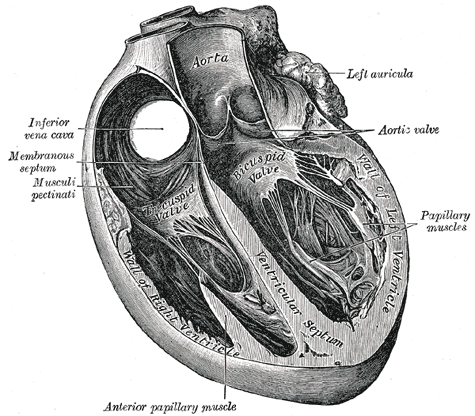
\includegraphics[width=0.7\textwidth]{figures/sample/Gray498.png} 
\caption[Four-chamber illustration of the human heart.]{Four-chamber illustration of the human heart.  Clockwise from upper-left: right atrium, left atrium, left ventricle, right ventricle.}
\label{fig:fourchamber}\end{figure}

The use of acoustic waves for medical diagnosis, inspired by naval sonar, was initially developed in the 1940s \cite{gagliardi_ultrasonography_1996}.  By 1954, the first clinically useful cardiac ultrasound -- examining motion of the mitral valve in stenosis -- was reported \cite{edler_ultrasonic_1957}.  These early scans were one-dimensional images (`A-mode'), sometimes repeated to generate a time axis (`M-mode').   The sector-scanning probe was developed in the 1970s \cite{bom_ultrasonic_1971,griffith_sector_1974}, leading to the `B-mode' that a modern cardiologist would recognise as an echocardiogram.



%% APPENDICES %% 
% Starts lettered appendices, adds a heading in table of contents, and adds a
%    page that just says "Appendices" to signal the end of your main text.
\cleardoublepage\phantomsection
\startappendices
\part*{Appendices}
\addcontentsline{toc}{part}{Appendices}
% Add or remove any appendices you'd like here:
% \begin{savequote}[8cm]
\textlatin{Cor animalium, fundamentum e\longs t vitæ, princeps omnium, Microco\longs mi Sol, a quo omnis vegetatio dependet, vigor omnis \& robur emanat.}

The heart of animals is the foundation of their life, the sovereign of everything within them, the sun of their microcosm, that upon which all growth depends, from which all power proceeds.
  \qauthor{--- William Harvey \cite{harvey_exercitatio_1628}}
\end{savequote}

\chapter{\label{app:1-cardiophys}Review of Cardiac Physiology and Electrophysiology}

\minitoc

Appendices are just like chapters.  Their sections and subsections get numbered and included in the table of contents; figures and equations and tables added up, etc.  Lorem ipsum dolor sit amet, consectetur adipiscing elit. Sed et dui sem. Aliquam dictum et ante ut semper. Donec sollicitudin sed quam at aliquet. Sed maximus diam elementum justo auctor, eget volutpat elit eleifend. Curabitur hendrerit ligula in erat feugiat, at rutrum risus suscipit. Pellentesque habitant morbi tristique senectus et netus et malesuada fames ac turpis egestas. Integer risus nulla, facilisis eget lacinia a, pretium mattis metus. Vestibulum aliquam varius ligula nec consectetur. Maecenas ac ipsum odio. Cras ac elit consequat, eleifend ipsum sodales, euismod nunc. Nam vitae tempor enim, sit amet eleifend nisi. Etiam at erat vel neque consequat.

\section{Anatomy}
\label{sec:anatomy}

Lorem ipsum dolor sit amet, consectetur adipiscing elit. Donec accumsan cursus neque. Pellentesque eget tempor turpis, quis malesuada dui. Proin egestas, sapien sit amet feugiat vulputate, nunc nibh mollis nunc, nec auctor turpis purus sed metus. Aenean consequat leo congue volutpat euismod. Vestibulum et vulputate nisl, at ultrices ligula. Cras pulvinar lacinia ipsum at bibendum. In ac augue ut ante mollis molestie in a arcu.

Etiam vitae quam sollicitudin, luctus tortor eu, efficitur nunc. Vestibulum maximus, ante quis consequat sagittis, augue velit luctus odio, in scelerisque arcu magna id diam. Proin et mauris congue magna auctor pretium id sit amet felis. Maecenas sit amet lorem ipsum. Proin a risus diam. Integer tempus eget est condimentum faucibus. Suspendisse sem metus, consequat vel ante eget, porttitor maximus dui. Nunc dapibus tincidunt enim, non aliquam diam vehicula sed. Proin vel felis ut quam porta tempor. Vestibulum elit mi, dictum eget augue non, volutpat imperdiet eros. Praesent ac egestas neque, et vehicula felis.

Pellentesque malesuada volutpat justo, id eleifend leo pharetra at. Pellentesque feugiat rutrum lobortis. Curabitur hendrerit erat porta massa tincidunt rutrum. Donec tincidunt facilisis luctus. Aliquam dapibus sodales consectetur. Suspendisse lacinia, ipsum sit amet elementum fermentum, nulla urna mattis erat, eu porta metus ipsum vel purus. Fusce eget sem nisl. Pellentesque dapibus, urna vitae tristique aliquam, purus leo gravida nunc, id faucibus ipsum magna aliquet ligula. Lorem ipsum dolor sit amet, consectetur adipiscing elit. Proin sem lacus, rutrum eget efficitur sed, aliquam vel augue. Aliquam ut eros vitae sem cursus ultrices ut ornare urna. Nullam tempor porta enim, in pellentesque arcu commodo quis. Interdum et malesuada fames ac ante ipsum primis in faucibus. Curabitur maximus orci purus, ut molestie turpis pellentesque ut.

Donec lacinia tristique ultricies. Proin dignissim risus ut dolor pulvinar mollis. Proin ac turpis vitae nibh finibus ullamcorper viverra quis felis. Mauris pellentesque neque diam, id feugiat diam vestibulum vitae. In suscipit dui eu libero ultrices, et sagittis nunc blandit. Aliquam at aliquet ex. Nullam molestie pulvinar ex vitae interdum. Praesent purus nunc, gravida id est consectetur, convallis elementum nulla. Praesent ex dolor, maximus eu facilisis at, viverra eget nulla. Donec ullamcorper ante nisi. Sed volutpat diam eros. Nullam egestas neque non tortor aliquet, sed pretium velit tincidunt. Aenean condimentum, est ac vestibulum mattis, quam augue congue augue, mattis ultrices nibh libero non ante. Lorem ipsum dolor sit amet, consectetur adipiscing elit.

Aenean volutpat eros tortor, non convallis sapien blandit et. Maecenas faucibus nulla a magna posuere commodo. Nullam laoreet ante a turpis laoreet malesuada. Phasellus in varius sem. Vestibulum sagittis nibh sed tincidunt blandit. Donec aliquam accumsan odio sit amet lacinia. Integer in tellus diam. Vivamus varius massa leo, vitae ullamcorper metus pulvinar sed. Maecenas nec lorem ornare, elementum est quis, gravida massa. Suspendisse volutpat odio ex, ac ultrices leo ultrices vel. Sed sed convallis ipsum. Pellentesque euismod a nulla sed rhoncus. Sed vehicula urna vitae mi aliquet, non sodales lacus ullamcorper. Duis mattis justo turpis, id tempus est tempus eu. Curabitur vitae hendrerit ligula.

Curabitur non pretium enim, in commodo ligula. Etiam commodo eget ligula a lacinia. Vestibulum laoreet ante tellus, vel congue sapien ornare in. Donec venenatis cursus velit vitae pulvinar. Pellentesque habitant morbi tristique senectus et netus et malesuada fames ac turpis egestas. Suspendisse in metus lectus. Pellentesque gravida dolor eget finibus imperdiet. Duis id molestie tortor. Mauris laoreet faucibus facilisis. Aliquam vitae dictum massa, sit amet dignissim lacus.

Fusce eleifend tellus id ex consequat maximus. Donec ultrices ex ut turpis ornare, non molestie mi placerat. Nulla sit amet auctor nunc, sit amet euismod elit. Phasellus risus tellus, condimentum a metus et, venenatis tristique urna. Cras mattis felis eget ipsum fermentum egestas. Ut augue odio, venenatis id convallis vel, congue quis augue. Maecenas sed maximus est, posuere aliquet tortor. Ut condimentum egestas nisi eu porttitor. Ut mi turpis, posuere id lorem vel, elementum tempor arcu.

Morbi nisl arcu, venenatis non metus ac, ullamcorper scelerisque justo. Nulla et accumsan lorem. Mauris aliquet dui sit amet libero aliquet, in ornare metus porttitor. Integer ultricies urna eu consequat ultrices. Maecenas a justo id purus ultricies posuere sed et quam. Cum sociis natoque penatibus et magnis dis parturient montes, nascetur ridiculus mus. Sed eleifend risus quis aliquet gravida. Nullam ac erat porta est bibendum dictum in a dolor. Nam eget turpis viverra, vulputate lectus eget, mattis ligula. Nam at tellus eget dui lobortis sodales et ut augue. In vestibulum diam eget mi cursus, ut tincidunt nulla pellentesque.

Aliquam erat volutpat. Sed ultrices massa id ex mattis bibendum. Nunc augue magna, ornare at aliquet gravida, vehicula sed lorem. Quisque lobortis ipsum eu posuere eleifend. Duis bibendum cursus viverra. Nam venenatis elit leo, vitae feugiat quam aliquet sed. Cras velit est, tempus ac lorem sed, pharetra lobortis ipsum. Donec suscipit gravida interdum. Nunc non finibus est. Nullam turpis elit, tempus non ante.

\section{Mechanical Cycle}

Lorem ipsum dolor sit amet, consectetur adipiscing elit. Aenean tellus est, suscipit sed facilisis quis, malesuada at ipsum. Nam tristique urna quis quam iaculis, et mattis orci pretium. Praesent euismod elit vel metus commodo ultrices. Vestibulum et tincidunt ex, in molestie ex. Donec ullamcorper sollicitudin accumsan. Etiam ac leo turpis. Duis a tortor felis. Nullam sollicitudin eu purus ac hendrerit. Nam hendrerit ligula libero, eget finibus orci bibendum a. Aenean ut ipsum magna.

Ut viverra, sapien sed accumsan blandit, nisi sem tempus tellus, at suscipit magna erat ornare nunc. Proin lacinia, nisi ut rutrum malesuada, nibh quam pellentesque nunc, sit amet consectetur purus felis ac tortor. Suspendisse lacinia ipsum eu sapien pellentesque mattis. Mauris ipsum nunc, placerat non diam vel, efficitur laoreet nunc. Sed lobortis, ipsum eget gravida facilisis, sem nulla viverra mi, in placerat eros sem viverra lacus. Aliquam porta aliquet diam vel commodo. Nulla facilisi. Duis erat libero, lobortis vel hendrerit vitae, sagittis id dui. Nulla pretium eros nec quam tincidunt, vel luctus mi aliquam. Integer imperdiet purus in est tristique venenatis. Ut pellentesque, nunc vitae iaculis ultricies, urna turpis dignissim risus, a laoreet felis magna nec erat.

Quisque sollicitudin faucibus ligula, et egestas nibh dictum sit amet. Proin eu mi a lectus congue pretium eu quis arcu. Suspendisse vehicula libero eu ipsum aliquam, vel elementum nibh mattis. Sed sed sapien vitae turpis tristique pulvinar a ut metus. Etiam semper gravida est, mollis gravida est porta ac. Proin eget tincidunt erat. Maecenas ultrices erat eget purus ultricies, ut lacinia arcu dictum. Nam et nisi sit amet ex congue mattis vel eget lorem. Aliquam erat volutpat. Pellentesque porttitor nibh vitae elementum consectetur. Aenean et est lobortis, congue sapien non, ullamcorper sapien. Ut facilisis sem non dapibus vehicula.

Mauris euismod odio dolor, sit amet gravida mauris placerat et. Curabitur nec dolor non nibh molestie lobortis dignissim non ante. Nullam rutrum lobortis ultrices. Aenean ex erat, elementum sed maximus id, posuere id quam. Proin rutrum ex elit, pretium aliquam risus finibus at. Aenean egestas orci velit, sed aliquet sapien condimentum a. Duis consequat, arcu eu viverra venenatis, dolor lorem gravida lectus, non aliquet nisi sem at augue. Donec laoreet blandit luctus. Aenean vehicula nisl vel faucibus luctus. Sed ut semper velit, vitae laoreet magna. Sed at interdum magna.

Sed iaculis faucibus odio, eu aliquam purus efficitur vel. Cras at nulla ac enim congue varius ut et nulla. Integer blandit mattis augue.

\section{Electrical Cycle}
\label{sec:electcycle}

Lorem ipsum dolor sit amet, consectetur adipiscing elit. In faucibus condimentum rhoncus. Ut dictum nisl id risus gravida lobortis. Sed vehicula mollis tellus ut varius. Fusce eget egestas dui, et commodo dui. Proin sollicitudin interdum tempus. Nullam in elit a enim fringilla bibendum. Vestibulum sodales pellentesque condimentum. Nulla facilisi. Nunc et dolor in nulla eleifend dictum at vel ligula. Aliquam ut velit non elit ullamcorper porta ac et ex. Fusce ornare magna non nunc vestibulum, eget molestie quam dictum. In interdum aliquam odio, in posuere tellus convallis quis. Curabitur non diam elit. Proin vulputate orci diam, a tincidunt ante luctus eu. Ut a viverra ligula. Curabitur pulvinar tempus tellus eget suscipit.

Aliquam posuere massa at ante dapibus congue. Curabitur ullamcorper tortor eget consectetur aliquet. Mauris tempor magna id mauris fringilla, a varius erat blandit. Nam eleifend ullamcorper placerat. Phasellus augue tortor, volutpat bibendum lorem nec, fringilla volutpat nisl. Mauris cursus urna metus, vel eleifend orci iaculis ut. Sed sit amet scelerisque massa, quis consequat dui. Donec semper sem dui, ac placerat velit egestas vel. Nulla facilisi. Quisque tellus eros, sagittis malesuada augue ut, faucibus dictum nulla. Vestibulum non dapibus erat, ut consequat libero. Ut turpis mi, dapibus commodo libero lobortis, maximus vestibulum lectus. Vestibulum sit amet sapien dapibus, tincidunt leo in, suscipit arcu. Sed in erat bibendum, laoreet eros eu, pellentesque justo. Nulla sodales purus neque, eget maximus ipsum consequat at. Maecenas a nisl sagittis, tempus ipsum sed, dictum mauris.

Suspendisse posuere odio lacus, at auctor tortor vehicula sed. Phasellus suscipit ornare enim vitae placerat. Sed viverra purus vel sapien tempor, quis iaculis erat laoreet. Aenean vel nunc vestibulum, ornare nunc ac, mollis urna. Aenean ultrices felis ipsum, ac semper est ullamcorper in. Donec in justo varius, egestas tortor ut, venenatis augue. Duis mattis, ligula quis lacinia fringilla, tellus neque accumsan ipsum, vitae tempor metus elit vel nibh. Curabitur porttitor urna nec sapien tempor, et porttitor velit malesuada.

Suspendisse aliquam nisl quis placerat vulputate. Proin dapibus ipsum ac ante sagittis, volutpat auctor sem dapibus. Nam in facilisis odio. Integer ante mauris, eleifend et pulvinar in, venenatis quis ligula. Phasellus posuere sollicitudin tortor eget euismod. Maecenas mollis tortor eget justo vulputate sagittis. Etiam hendrerit massa quis ex molestie sodales. Quisque facilisis erat lacus, id convallis sem suscipit bibendum. Integer dui urna, pharetra sed porta sed, bibendum ut odio. Donec placerat at lectus egestas consequat. Sed id rhoncus est, vitae vulputate sapien. Fusce tempus quam lorem, id ornare turpis sodales sed. Integer aliquet urna eget condimentum consequat. Vestibulum quis dui vel ligula posuere luctus id nec turpis.

Nam vitae placerat lacus. Mauris scelerisque interdum volutpat. Nunc aliquet tristique enim, sit amet molestie felis ullamcorper vitae. Nullam sollicitudin orci orci, in condimentum tellus consectetur in. Nam id justo justo. Fusce eget finibus est. Proin id tortor nec quam cursus vehicula. Aliquam ultrices eros eros, a tincidunt elit eleifend auctor.

Nullam consectetur dapibus ligula sit amet efficitur. Nunc non posuere sapien. Vivamus dui nisl, aliquam id ipsum non, pulvinar ornare neque. Nunc rhoncus pretium congue. Fusce id laoreet enim. Cras sed massa in eros bibendum auctor in nec sem. Nam commodo, velit id porta consequat, mi arcu gravida lorem, ut aliquam elit ante quis dui. Quisque in massa sed nibh blandit dictum.

Vestibulum molestie consectetur porttitor. Donec tincidunt vel orci at pharetra. Nullam id felis sit amet nulla tempus lacinia. Integer egestas ullamcorper massa, ut ultricies diam congue sit amet. Cras sit amet velit at nibh vehicula finibus a et lorem. Cras odio metus, venenatis ut ultrices non, ornare ac orci. Morbi et nulla dui. Mauris dictum molestie nibh, eu efficitur lorem accumsan quis.

\section{Cellular Electromechanical Coupling}
\label{sec:electromech}

Lorem ipsum dolor sit amet, consectetur adipiscing elit. Nullam vitae consectetur metus, ac maximus ex. Quisque vitae ex eu lectus ultricies consequat vel non lorem. Etiam odio ipsum, tempus ut lobortis in, molestie ac leo. Vivamus mollis feugiat bibendum. Vestibulum eget venenatis quam. Aenean faucibus, massa sed ullamcorper porta, arcu nunc iaculis velit, quis consectetur purus neque placerat nibh. Vestibulum elit nunc, dignissim vulputate venenatis et, sodales non massa. Proin leo ligula, vehicula eu aliquam varius, posuere a dolor. Donec iaculis auctor neque, sit amet gravida libero porta vel. Vivamus consequat elementum lacus, at bibendum mauris egestas nec. Fusce fermentum diam eu dolor ornare, vitae vestibulum leo interdum. Morbi luctus libero quis dictum laoreet. Etiam semper porta ante, vel ullamcorper enim sodales quis.

Nullam eu nisi faucibus, fermentum ex auctor, tempor arcu. Phasellus condimentum erat mi, condimentum malesuada ligula congue venenatis. Nullam gravida imperdiet urna quis cursus. Ut tempus nec purus eget posuere. Cras non nulla sit amet justo aliquet pellentesque nec sed eros. Nam aliquam nisl urna, in placerat magna gravida venenatis. Donec interdum vel magna ullamcorper molestie. Nunc felis neque, rhoncus fringilla faucibus sit amet, ultrices sed magna. Maecenas malesuada hendrerit diam in ultrices. Nam libero urna, volutpat ut auctor eget, interdum sed odio. Vestibulum suscipit mauris nec augue ornare, ut eleifend nulla gravida. Proin imperdiet, mauris quis consectetur porta, leo dui convallis leo, id lobortis massa diam eu libero. Aenean hendrerit vel ante aliquam venenatis. Pellentesque bibendum pretium odio, ut sagittis lectus feugiat a. Donec porttitor vulputate lacus.

Nunc volutpat efficitur lacus in aliquet. Nullam non iaculis diam, at ultrices diam. Proin vehicula vulputate cursus. Morbi tempus sapien id urna lobortis interdum. Maecenas elementum sagittis elementum. Donec at sodales velit, a posuere tortor. Nulla id hendrerit tortor. Sed semper velit in magna sagittis pulvinar. Nulla nec arcu molestie, ultricies sapien sit amet, sollicitudin nisi. Donec nisi massa, suscipit ut dignissim quis, lacinia id leo.

Suspendisse ut mi metus. Morbi tincidunt ligula in porttitor consectetur. Integer eu urna urna. Suspendisse potenti. Mauris sit amet felis eu diam auctor ullamcorper. Morbi in porta nisi. Nam ante tortor, venenatis vitae tempor sed, sagittis vitae velit. In semper orci sit amet nisi ullamcorper varius. Aenean dignissim ultrices imperdiet. Maecenas lacinia enim id neque porttitor iaculis. Curabitur laoreet ante ut urna dignissim, id sollicitudin metus consectetur. Aenean massa ipsum, auctor vel ante vel, blandit dignissim libero. Fusce interdum ac magna et interdum.

\begin{savequote}[8cm]
‘After all, it is a common weakness of young authors to put too much into their papers.’

  \qauthor{--- Ronald Fisher, \textit{\usebibentry{fisher1950contributions}{title}} \citeyearpar{fisher1950contributions}}
\end{savequote}

% \chapter{\label{app:list-hostpots}Human and mouse recombination hotspots individually analysed with sperm-typing studies}
\chapter{\label{app:data-and-figs}Supplementary data and figures}

\minitoc{}

\section{Supplementary data}
\subsection{PRDM9\textsuperscript{Dom2/Cst}-targeted hotspots studied}

The table below gives the list of mouse hotspots targeted by either PRDM9\textsuperscript{Dom2} or PRDM9\textsuperscript{Cst} that have been individually studied.


\begin{table}[h]
    \centering
	\begin{adjustbox}{width = 1\textwidth}
    \begin{tabular}{rrrr}
        \toprule
        \textbf{Name} & \textbf{Target allele} & \textbf{Chromosome} & \textbf{Reference} \\

        % \textbf{category} & \textbf{targets} & \textbf{fragments} & \textbf{events} & \textbf{($\times$ 10\textsuperscript{-6})} \\

        \midrule
        A3 & PRDM9\textsuperscript{Dom2} & 1 & \citet{kelmenson2005torrid, cole2010comprehensive} \\
        G7c & PRDM9\textsuperscript{Dom2} & 17 & \citet{snoek1998molecular} \\
        E\textsubscript{\textgreek{β}} & PRDM9\textsuperscript{Dom2} & 17 & \citet{steinmetz1982molecular} \\ % strain B6
        Esrrg1 & PRDM9\textsuperscript{Cst} & 1 & \citet{billings2013dna} \\
        Hlx1 & PRDM9\textsuperscript{Cst} & 1 & \citet{ng2008quantitative,billings2013dna} \\
        HS9 & PRDM9\textsuperscript{Dom2} & 19 & \citet{bois2007highly,getun2010nucleosome} \\%B6/DBA2 strain
        HS22 & PRDM9\textsuperscript{Dom2} & 19 & \citet{getun2010nucleosome} \\
        HS59.4 & PRDM9\textsuperscript{Dom2} & 19 & \citet{getun2010nucleosome} \\
        HS61.1 & PRDM9\textsuperscript{Dom2} & 19 & \citet{wu2010anatomy,getun2010nucleosome} \\
        Pbx1 & PRDM9\textsuperscript{Dom2} & 1 & \citet{billings2013dna,baker2015multimer} \\
        Psmb9 & PRDM9\textsuperscript{Cst} & 17 & \citet{guillon2002initiation,baudat2007cis} \\
        \bottomrule
    \end{tabular}
	\end{adjustbox}
    \caption[List of PRDM9\textsuperscript{Dom2}- and PRDM9\textsuperscript{Cst}-targeted hotspots individually studied]
    {\textbf{List of PRDM9\textsuperscript{Dom2}- and PRDM9\textsuperscript{Cst}-targeted hotspots individually studied.}
    }
\label{tab:hotspots-studied-sperm-typing}
\end{table}


\subsection{Disclaimer for the resources used}
% https://www.ncbi.nlm.nih.gov/pmc/articles/PMC4389181/
% The ensuing 25 years saw the number of identified mammalian hot spots increase incrementally, often by chance. The list of recognized hot spots now includes Ath1 (also known as Tnfsf4)9, Scnm1 (REF. 10) and the HS22 region11 in mice, at least four hot spots in the H2 region12,

This work was performed using the computing facilities of the CC LBBE/PRABI\@.


\subsection{Estimation of erroneous W\textrightarrow{} S and S\textrightarrow{} W conversion events}

Quantifying gBGC comes back to measuring the $\frac{WS}{WS+SW}$ ratio.
However, since the large majority of pot-NCO-1 events corresponded to FPs, we had to distinguish the (potential) contribution of FPs to this ratio from that of genuine NCO-1 events.
In particular, this ratio may depart from the expected 50\% ratio if (1) a non-negligible proportion of FPs arise from sequencing miscalls and (2) W\textrightarrow{} S and S\textrightarrow{} W sequencing errors appear at different frequencies.\\

% \paragraph{Proportion of FPs due to sequencing errors\\}
First, we thus wanted to quantify the proportion of FPs due to sequencing miscalls.
To do this, we estimated the sequencing error rate directly in our sequencing data by monitoring the apparition of \textit{de novo} variants:
given that the mutation rate ($\sim$10\textsuperscript{-8}/bp) is much lower than the sequencing error rate ($\sim$10\textsuperscript{-3}/bp), we assumed that, outside the polymorphic sites identified by variant-calling, any base call that differed from the nucleotide of the reference genome was a sequencing error and counted them to compute the conditional frequency matrix of sequencing errors\footnote{Matrix $M$ was computed based on the analysis of one chromosome (chromosome 10) for all of our 18 samples individually (because the sequencing errors may vary between the biological samples and sequencing runs). This matrix gives the probability of each erroneous base call, given the genuine nucleotide.} ($M$):

\begin{equation*}
M = \begin{bmatrix}
\Pr( A\rightarrow A \mid A) & \Pr( A\rightarrow C \mid A) & \Pr( A\rightarrow G \mid A) & \Pr( A\rightarrow T \mid A) \\
\Pr( C\rightarrow A \mid C) & \Pr( C\rightarrow C \mid C) & \Pr( C\rightarrow G \mid C) & \Pr( C\rightarrow T \mid C) \\
\Pr( G\rightarrow A \mid G) & \Pr( G\rightarrow C \mid G) & \Pr( G\rightarrow G \mid G) & \Pr( G\rightarrow T \mid G) \\
\Pr( T\rightarrow A \mid T) & \Pr( T\rightarrow C \mid T) & \Pr( T\rightarrow G \mid T) & \Pr( T\rightarrow T \mid T) 
\end{bmatrix}
\end{equation*}






$\forall (i,j) \in \{A, C, G, T\}^2$, the number of NCO-1 FPs expected due to sequencing errors involving a genuine base $i$ mistakenly called as a $j$ base ($e_{i\rightarrow j}$) simply equalled the product of the number of central markers (i.e.\ markers \textit{not} located at the extremity of fragments) that were genuinely $i$ in $ij$ polymorphic sites ($g_{i}^{ij}$) by the conditional probability that a genuine $i$ would mistakenly be called a $j$ ($\Pr( i\rightarrow j \mid i )$):

\begin{equation} \label{eq:nb-errors}
	e_{i\rightarrow j} = g_{i}^{ij} \times \Pr( i\rightarrow j \mid i )
\end{equation}


$g_{i}^{ij}$ was not directly accessible from the data because we could not know which base calls were correctly sequenced.
Though, this number was linked to the number of central markers containing an $i$ allele and involved in a polymorphic site $ij$ ($n_{i}^{ij}$) through the following equation:

\begin{equation} \label{eq:genuine-to-called}
	n_{i}^{ig} = g_{i}^{ij} \times ( 1 - \Pr( i\rightarrow j \mid i ) ) + g_{j}^{ij} \times \Pr( j\rightarrow i \mid j )
\end{equation}


When we computed the $M$ matrix, we found that the frequency of sequencing errors was very low ($\simeq 10^{-3}$).
Thus, to approximate $g_{i}^{ij}$, we used the simplifying assumption that the frequency of wrong calls were close to zero and that of good calls close to 1:

\begin{subequations} 
	\begin{alignat}{5}
		\forall &(i,j) &{}\in{}& \{A, C, G, T\}^2 \; \backslash \: i \neq j, &{}\Pr({}& i\rightarrow j \mid i ) \simeq 0,\label{eq:assumption-low-freqs}\\
		\forall &i	   &{}\in{}& \{A, C, G, T\},							 &{}\Pr({}& i\rightarrow i \mid i ) \simeq 1
	\end{alignat}
\end{subequations}


From equation~\ref{eq:assumption-low-freqs}, equation~\ref{eq:genuine-to-called} simplified to:

\begin{equation} \label{eq:genuine-to-called-simplified}
	n_{i}^{ij} \simeq g_{i}^{ij}
\end{equation}

And, by incorporating equation~\ref{eq:genuine-to-called-simplified} into equation~\ref{eq:nb-errors}, we had:

\begin{equation*} \label{eq:nb-errors-with-only-known-parameters}
	e_{i\rightarrow j} = n_{i}^{ij} \times \Pr( i\rightarrow j \mid i )
\end{equation*}


Finally, the total number of FPs that were expected due to sequencing errors ($E$) was the total sum of each type of sequencing error: 

\begin{equation*} \label{eq:sum-all-NCOs-expected}
	E = \underset{i \neq j} {\sum_{(i, j) \in \{A, C, G, T\}^2}} e_{i\rightarrow j}
\end{equation*}




This allowed us to predict that, among the total 287,577,349 fragments overlapping 3 markers or more, 231,905 were expected to be discovered as NCO-1 FPs due to sequencing errors only.
This represented 66.7\% of the 347,652\footnote{The sequencing error estimate was calculated upon all sequenced fragments, i.e.\ before setting the sequencing error filter, and thus had to be compared to the total number of NCO-1 FPs obtained without the filter (Table~\ref{tab:NCO-1-FP-rate-no-filter}).} NCO-1 FPs that we found in pot-NCO-1 events (110,615 in control regions + an estimate of 237,037 in hotspots, Table~\ref{tab:NCO-1-FP-rate-no-filter}).


\begin{table}[t]
    \centering
    % \begin{adjustbox}{width = 1\textwidth}
		\begin{tabular}{rrrrr}
            \toprule
            \textbf{Target} & \textbf{Nb of} & \textbf{Nb of} & \textbf{Nb of} & \textbf{Event rate} \\

            \textbf{category} & \textbf{targets} & \textbf{fragments} & \textbf{events} & \textbf{($\times$ 10\textsuperscript{-6})} \\

            \midrule
            Hotspots & 1,018 & 228,984,512 & 243,390 & 1062.9 \\
            Controls & 500 & 106,850,906 & 110,615 & 1035.2 \\
            \midrule
            \multicolumn{1}{r}{\textbf{FP rate}} & \multicolumn{4}{r}{\textbf{97.4 \%}} \\
            \bottomrule
        \end{tabular}
    % \end{adjustbox}
    \caption[Number of pot-NCO-1 events detected in hotspot and control targets without the sequencing error filter]
    {\textbf{Number of pot-NCO-1 events detected in hotspot and control targets without the sequencing error filter.}
        \par Pot-NCO-1 events were detected without the sequencing error filter controlling that the allele supporting the genotype call with the mapping onto the B6 genome is identical to that based on the mapping onto the CAST genome.
        All fragments or events overlapping at least 1 bp with a given target are counted in this table.
        The event rate corresponds to the ratio of candidate recombination events over the total number of fragments.
        The maximum false positive (FP) rate is the ratio of the event rate in control targets over that in hotspots.
    }
\label{tab:NCO-1-FP-rate-no-filter}
\end{table}



We further evaluated the imprecision on this percentage by calculating, for each sample individually\footnote{With the exception of the four samples which were lowly sequenced}, the ratio between the latter number of FPs expected in the sample due to sequencing errors and the total number of fragments in the sample. 
We sequentially applied the multiplier of each sample to the total number of fragments and finally determined that the proportion of FPs due to sequencing errors capped between 60 and 78\% of all FPs.\\


Therefore, the largest part (66.7\%, CI $= [60\%; 78\%$]) of FPs arose from sequencing errors.
The next step thus consisted in estimating the $\frac{WS}{WS+SW}$ ratio expected because of these sequencing errors.
To do this, we simply computed the total number of FPs containing an erroneous W\textrightarrow{} S base call ($E_{W\rightarrow S}$) and the number containing an erroneousS\textrightarrow{} W base call ($E_{S\rightarrow W}$) as follows:

\begin{align}
        E_{W\rightarrow S}&= e_{A\rightarrow C} + e_{A\rightarrow G} + e_{T\rightarrow C} + e_{T\rightarrow G}, \\
        E_{S\rightarrow W}&= e_{C\rightarrow A} + e_{C\rightarrow T} + e_{G\rightarrow A} + e_{G\rightarrow T}
\end{align}

Importantly, we found that $E_{S\rightarrow W}$ was greater than $E_{W\rightarrow S}$, i.e.\ S bases were more oftenly mistakenly sequenced as W bases than the other way round.
More precisely, we found that the $\frac{WS}{WS+SW}$ ratio expected with such FPs (i.e.\ $\frac{E_{W\rightarrow S}}{E_{W\rightarrow S} + E_{S\rightarrow W}}$) equalled 0.39.

We note that this estimate was slightly higher than the $\frac{WS}{WS+SW}$ observed in control regions (0.31), possibly because the non-negligible portion (33.3\%) of FPs that did not originate from these sequencing errors may somehow also bias the ratio.









% \subsection{Source code to reproduce figures}
%
% The source code to reproduce figures will be put online shortly.
%


% SRA et reproductibilite des figures
% mettre aussi la liste des positions genomiques obtenues

\hypersetup{linkcolor=titlepagecolorsection}
\section{Supplementary figures for Chapter~\ref{ch:6-recombination-parameters}}
\hypersetup{linkcolor=black}

\subsection{Recombination rate and DMC1 binding affinity}

\begin{figure}[h!]
    \centering
    \includegraphics[width = 1\textwidth]{figures/appendices/Correlation_intensity_DMC1.eps}
    \caption[Proportionality between the recombination rate and DMC1 binding intensity]
    {\textbf{Proportionality between the recombination rate and DMC1 binding intensity.}
        \par All 1,018 hotspots were divided into 10 classes of increasing DMC1 signal (x-axis), i.e.\ the number of DMC1 ChIP-seq tags on each PRDM9 ChIP-seq peak (DMC1 ChIP-seq data on B6xCAST hybrid mice from \citealp{smagulova2016evolutionary}).
        The observed number of recombination events identified per sequenced Mb (left y-axis) was converted into a CO rate (right y-axis) as detailed in Chapter~\ref{ch:6-recombination-parameters}.
        The points and error bars respectively represent the mean number of events (or CO rate) and the standard error on the mean for hotspots of each class.
    }
\label{fig:correlation-DMC1-standard-error}
\end{figure}



\subsection{Hotspot asymmetry and DMC1 binding affinity}


\begin{figure}[h!]
    \centering
    \includegraphics[width = 1\textwidth]{figures/appendices/Recombination_rates_2_axes_sym_vs_Asym_DMC1_with_legend_and_outliers-corrected_CO_x2.eps}
    \caption[Asymmetric hotspots display lower recombinational activity than expected by their DMC1 binding affinity]
    {\textbf{Asymmetric hotspots display lower recombinational activity than expected by their DMC1 binding affinity.}
        \par All 1,018 hotspots were divided into 10 classes of increasing DMC1 signal (x-axis), i.e.\ the number of DMC1 ChIP-seq tags on each DMC1 ChIP-seq peak (DMC1 ChIP-seq data on B6xCAST hybrid mice from \citealp{smagulova2016evolutionary}).
        The observed number of recombination events identified per sequenced Mb (left y-axis) was converted into a CO rate (right y-axis) as detailed in Chapter~\ref{ch:6-recombination-parameters}.
        Symmetric hotspots (green, $N = 650$) were distinguished from asymmetric hotspots (orange, $N = 236$) as detailed in Chapter~\ref{ch:7-quantification-BGC}.
        The linear regression model for symmetric (slope~$= 1.8$; intercept~$=0$; \textit{p}-val~$< 2.2 \times 10^{-16}$) and asymmetric (slope~$= 8.6$; intercept~$=0$; \textit{p}-val~$< 2.2 \times 10^{-16}$) hotspots are drawn as dotted lines.
    }
\label{fig:asymmetry-and-DMC1}
\end{figure}



\newpage
\subsection{Distribution of switch points}


\begin{figure}[h!]
    \centering
    \includegraphics[width = 1\textwidth]{figures/appendices/density_switch_points.eps}
    \caption[Distribution of switch points along hotspots for Rec-1S and Rec-2S events]
    {\textbf{Distribution of switch points along hotspots for Rec-1S and Rec-2S events.}
}
\label{fig:density-switch-points}
\end{figure}



\newpage
\hypersetup{linkcolor=titlepagecolorsection}
\section{Supplementary figures for Chapters~\ref{ch:7-quantification-BGC} and~\ref{ch:8-HFM1}}
\hypersetup{linkcolor=black}

\subsection{Correlation between expected and observed donor}



\begin{figure}[h!]
    \centering
    \includegraphics[width = 1\textwidth]{figures/appendices/CorrelationDMC1_FINAL_BIS_on_lab_computer_COLOURS.eps}
    \caption[Correlation between the expected and observed proportions of CAST-donor fragments across hotspots displaying at least 5 events, coloured per PRDM9 target]
    {\textbf{Correlation between the expected and observed proportions of CAST-donor fragments across hotspots displaying at least 5 events, coloured per PRDM9 target.}
        \par The expected proportion of CAST-donor fragments (x-axis) was based on the probability that the DSB initiates on the B6 haplotype from DMC1 ssDNA-sequencing (SSDS) data by \citet{smagulova2016evolutionary} (see main text).
        Only the 582 hotspots displaying a minimum of 5 recombination events were reported in this figure.
        The Pearson correlation between the two measures gave: $R^2 = 0.66$; {\textit{p}-val $< 2.2 \times 10^{-16}$}.
}
\label{fig:correl-donor-DMC1-with-colour}
\end{figure}



\subsection{Genetic background of all chromosomes}


% LEFT PAGE
\begin{sidewaysfigure}[p]
	\centering
	\leftskip-3.4cm
	\rightskip-2.7cm
	\rotfloatpagestyle{empty}
	\includegraphics[width = 1.25\textwidth]{figures/chap8/HFM1_background_28355.eps}
	\captionsetup{width=1.25\textwidth, margin={-2.2cm, -3.3cm}}
	\caption[Mosaic of genetic backgrounds inferred at each target along the chromosomes of mouse 28355]
	{\textbf{Mosaic of genetic backgrounds inferred at each target along the chromosomes of mouse 28355.}
		\par Chromosomes are represented in grey and oriented so that the centromere is on the bottom side of the figure (mouse chromosomes are acrocentric).
		Each segment corresponds to the position of a target (hotspot or control region) and was coloured in red when the background inferred was BD/BD (homozygous) and in blue when the background inferred was BD/CAST (heterozygous).
	}
\label{fig:mosaic-backgrounds}
\end{sidewaysfigure}


% RIGHT PAGE
\begin{sidewaysfigure}[p]
	\centering
	\leftskip-2.4cm
	\rightskip-2.4cm
	\rotfloatpagestyle{empty}
	\includegraphics[width = 1.25\textwidth]{figures/chap8/HFM1_background_28367.eps}
	\captionsetup{width=1.25\textwidth, margin={-2.2cm, -3.3cm}}
	\caption[Mosaic of genetic backgrounds inferred at each target along the chromosomes of mouse 28367]
	{\textbf{Mosaic of genetic backgrounds inferred at each target along the chromosomes of mouse 28367.}
		\par Chromosomes are represented in grey and oriented so that the centromere is on the bottom side of the figure (mouse chromosomes are acrocentric).
		Each segment corresponds to the position of a target (hotspot or control region) and was coloured in red when the background inferred was BD/BD (homozygous) and in blue when the background inferred was BD/CAST (heterozygous).
	}
\label{fig:mosaic-backgrounds}
\end{sidewaysfigure}


% LEFT PAGE
\begin{sidewaysfigure}[p]
	\centering
	\leftskip-3.4cm
	\rightskip-2.7cm
	\rotfloatpagestyle{empty}
	\includegraphics[width = 1.25\textwidth]{figures/chap8/HFM1_background_28371.eps}
	\captionsetup{width=1.25\textwidth, margin={-2.2cm, -3.3cm}}
	\caption[Mosaic of genetic backgrounds inferred at each target along the chromosomes of mouse 28371]
	{\textbf{Mosaic of genetic backgrounds inferred at each target along the chromosomes of mouse 28371.}
		\par Chromosomes are represented in grey and oriented so that the centromere is on the bottom side of the figure (mouse chromosomes are acrocentric).
		Each segment corresponds to the position of a target (hotspot or control region) and was coloured in red when the background inferred was BD/BD (homozygous) and in blue when the background inferred was BD/CAST (heterozygous).
	}
\label{fig:mosaic-backgrounds}
\end{sidewaysfigure}





\newpage
% \subsection{Pairwise recombination rates of shared hotspots}
\subsection{Pairwise comparison of the RR in shared hotspots}



\begin{figure}[p]
    \centering
    \begin{subfigure}[b]{0.75\textwidth}
        \subcaption{Between 28371 (WT) and 28353 (mutant)}
        \includegraphics[width=\textwidth]{figures/chap8/28371_vs_28353.eps}
    \end{subfigure}

    \vspace{0.5cm}

    \begin{subfigure}[b]{0.75\textwidth}
        \subcaption{Between 28371 (WT) and 28367 (mutant)}
        \includegraphics[width=\textwidth]{figures/chap8/28371_vs_28367.eps}
    \end{subfigure}

    \caption[Correlation of the number of recombination events in shared hotspots for all pairs of mice]
    {\textbf{Correlation of the number of recombination events in shared hotspots for all pairs of mice.}
        % \par The linear regression was significant for the WT mice (slope $=1.03$; \textit{p}-val $< 2 \times 10^{-16}$; $n_{hotspots} = 257$) and for the two mutant mice (slope = $0.69$; \textit{p}-val $< 2 \times 10^{-16}$; $n_{hotspots} = 241$).
    }
\label{fig:pairwise-RR-shared-BIS-1}
\end{figure}




\begin{figure}[p]
    \centering
   
	\begin{subfigure}[b]{0.75\textwidth}
        \subcaption{Between 28355 (WT) and 28367 (mutant)}
        \includegraphics[width=\textwidth]{figures/chap8/28355_vs_28367.eps}
    \end{subfigure}

    \vspace{0.5cm}
    
	\begin{subfigure}[b]{0.75\textwidth}
        \subcaption{Between 28355 (WT) and 28353 (mutant)}
        \includegraphics[width=\textwidth]{figures/chap8/28355_vs_28353.eps}
    \end{subfigure}


    \caption[Correlation of the number of recombination events in shared hotspots for all pairs of mice]
    {\textbf{Correlation of the number of recombination events in shared hotspots for all pairs of mice.}
        % \par The linear regression was significant for the WT mice (slope $=1.03$; \textit{p}-val $< 2 \times 10^{-16}$; $n_{hotspots} = 257$) and for the two mutant mice (slope = $0.69$; \textit{p}-val $< 2 \times 10^{-16}$; $n_{hotspots} = 241$).
    }
\label{fig:pairwise-RR-shared-BIS2}
\end{figure}







% + liste de tous les hotspots analyses chez les humains (ou pour moi, plutot souris) dans annexe B de Popa.



%%% CHAPITRE 2
%% Si je veux metttre une appendix sur les defects des souris qui sont mutantes pour un gene de la meiose: Bolcun-Filas, E., & Schimenti, J. C. (2012). Genetics of Meiosis and Recombination in Mice. International Review of Cell and Molecular Biology, 179–227. doi:10.1016/b978-0-12-394309-5.00005-5 (appendix)




%%%%% REFERENCES

% JEM: Quote for the top of references (just like a chapter quote if you're using them).  Comment to skip.
% \begin{savequote}[8cm]
% The first kind of intellectual and artistic personality belongs to the hedgehogs, the second to the foxes \dots
%   \qauthor{--- Sir Isaiah Berlin \cite{berlin_hedgehog_2013}}
% \end{savequote}
%
\setlength{\baselineskip}{0pt} % JEM: Single-space References

% {\renewcommand*\MakeUppercase[1]{#1}%
% \printbibliography[heading=bibintoc,title={\bibtitle}]}

\renewcommand\bibname{References}
\bibliographystyle{apalike}
\bibliography{references,bibliography_additional/Bibtex/01_chronology_recombination,bibliography_additional/Bibtex/chap3_RR_variation_and_evolution,bibliography_additional/Bibtex/chap4_gBGC,bibliography_additional/Bibtex/chap5_methodology}

\end{document}
